\PassOptionsToPackage{enable-debug,check-declarations}{expl3}
\RequirePackage{pdfmanagement-testphase}
\DeclareDocumentMetadata {  }
\ExplSyntaxOn
\pdfmanagement_add:nnn{Catalog}{Lang}{(enUS)}
\ExplSyntaxOff

% xmp metadata for pdf
% Originally used \usepackage[a-2a]{pdfx}
% \usepackage{hyperxmp} replaced it
% \RequirePackage{pdfmanagement-testphase} replaced it

\documentclass[11pt,
  english,
  a4paper,
]{article}
\usepackage{sa4ss}
\usepackage{amsmath,amssymb,array}
\usepackage{booktabs}

% From tagged-template.latex
\usepackage{lmodern}
\usepackage{ifxetex,ifluatex}
\ifnum 0\ifxetex 1\fi\ifluatex 1\fi=0 % if pdftex
  \usepackage[T1]{fontenc}
  \usepackage[utf8]{inputenc}
  \usepackage{textcomp} % provide euro and other symbols
\else % if luatex or xetex
  \usepackage{unicode-math}
  \defaultfontfeatures{Scale=MatchLowercase}
  \defaultfontfeatures[\rmfamily]{Ligatures=TeX,Scale=1}
\fi

% Use upquote if available, for straight quotes in verbatim environments
\IfFileExists{upquote.sty}{\usepackage{upquote}}{}
\IfFileExists{microtype.sty}{% use microtype if available
  \usepackage[]{microtype}
  \UseMicrotypeSet[protrusion]{basicmath} % disable protrusion for tt fonts
}{}
\makeatletter
\@ifundefined{KOMAClassName}{% if non-KOMA class
  \IfFileExists{parskip.sty}{%
    \usepackage{parskip}
  }{% else
    \setlength{\parindent}{0pt}
    \setlength{\parskip}{6pt plus 2pt minus 1pt}}
}{% if KOMA class
  \KOMAoptions{parskip=half}}
\makeatother
\usepackage{xcolor}
\IfFileExists{xurl.sty}{\usepackage{xurl}}{} % add URL line breaks if available
\hypersetup{
  pdftitle={Status of vermilion rockfish (Sebastes miniatus) off the waters of Oregon state.},
  pdflang={en},
  hidelinks,
  pdfcreator={LaTeX via pandoc}}
\urlstyle{same} % disable monospaced font for URLs
\usepackage{longtable}
% Correct order of tables after \paragraph or \subparagraph
\usepackage{etoolbox}
\makeatletter
\patchcmd\longtable{\par}{\if@noskipsec\mbox{}\fi\par}{}{}
\makeatother
% Allow footnotes in longtable head/foot
\IfFileExists{footnotehyper.sty}{\usepackage{footnotehyper}}{\usepackage{footnote}}
\makesavenoteenv{longtable}
\usepackage{graphicx}
\makeatletter
\def\maxwidth{\ifdim\Gin@nat@width>\linewidth\linewidth\else\Gin@nat@width\fi}
\def\maxheight{\ifdim\Gin@nat@height>\textheight\textheight\else\Gin@nat@height\fi}
\makeatother
% Scale images if necessary, so that they will not overflow the page
% margins by default, and it is still possible to overwrite the defaults
% using explicit options in \includegraphics[width, height, ...]{}
\setkeys{Gin}{width=\maxwidth,height=\maxheight,keepaspectratio}
% Set default figure placement to htbp
\makeatletter
\def\fps@figure{htbp}
\makeatother
\setlength{\emergencystretch}{3em} % prevent overfull lines
\providecommand{\tightlist}{%
  \setlength{\itemsep}{0pt}\setlength{\parskip}{0pt}}
\setcounter{secnumdepth}{5}
\ifxetex
  % Load polyglossia as late as possible: uses bidi with RTL langages (e.g. Hebrew, Arabic)
  \usepackage{polyglossia}
  \setmainlanguage[]{english}
\else
  \usepackage[shorthands=off,main=english]{babel}
\fi

%Define cslreferences environment, required by pandoc 2.8
%https://github.com/rstudio/rmarkdown/issues/1649
\newlength{\csllabelwidth}
\setlength{\csllabelwidth}{3em}
\newlength{\cslhangindent}
\setlength{\cslhangindent}{1.5em}
% for Pandoc 2.8 to 2.10.1
\newenvironment{cslreferences}%
  {}%
  {\par}
% For Pandoc 2.11+
\newenvironment{CSLReferences}[2] % #1 hanging-ident, #2 entry spacing
 {% don't indent paragraphs
  \setlength{\parindent}{0pt}
  % turn on hanging indent if param 1 is 1
  \ifodd #1 \everypar{\setlength{\hangindent}{\cslhangindent}}\ignorespaces\fi
  % set entry spacing
  \ifnum #2 > 0
  \setlength{\parskip}{#2\baselineskip}
  \fi
 }%
 {}
\usepackage{calc}  % for \widthof, \maxof in minipage
\newcommand{\CSLBlock}[1]{#1\hfill\break}
\newcommand{\CSLLeftMargin}[1]{\parbox[t]{\csllabelwidth}{#1}}
\newcommand{\CSLRightInline}[1]{\parbox[t]{\linewidth - \csllabelwidth}{#1}\break}
\newcommand{\CSLIndent}[1]{\hspace{\cslhangindent}#1}


\providecommand{\tightlist}{%
  \setlength{\itemsep}{0pt}\setlength{\parskip}{0pt}}


\date{}
\newcommand{\trTitle}{Status of vermilion rockfish (\emph{Sebastes miniatus}) off the waters of Oregon state.}
\newcommand{\trYear}{2021}
\newcommand{\trMonth}{July}
\newcommand{\trAuthsLong}{truetrue}
\newcommand{\trAuthsBack}{Cope, J.M., A.D. Whitman}
\newcommand{\trCitation}{
\begin{hangparas}{1em}{1}
\trAuthsBack{}. \trYear{}. \trTitle{}. Pacific Fisheries Management Council, Portland, Oregon. \pageref{LastPage}{}\,p.
\end{hangparas}}

\AtBeginDocument{\tagstructbegin{tag=Document}}
\AtEndDocument{\tagstructend}
\pretocmd{\maketitle}{\tagstructbegin{tag=H1}\tagmcbegin{tag=H1}}{}{}
\apptocmd{\maketitle}{\tagmcend\tagstructend}{}{}

\begin{document}

%%%%% Frontmatter %%%%%

% Footnote symbols in front matter
\renewcommand*{\thefootnote}{\fnsymbol{footnote}}

\small
\thispagestyle{empty}
\pagenumbering{roman}
\noindent
\begin{center}
\title{Status of vermilion rockfish (\emph{Sebastes miniatus}) off the waters of Oregon state.}
% \textnormal{\MakeTextUppercase{\trTitle{}}}
\vspace{1.5cm}
{\Large\textbf\newline{Status of vermilion rockfish (\emph{Sebastes miniatus}) off the waters of Oregon state.}}
\vfill
by\\
Jason M. Cope\textsuperscript{1}\\
Alison D. Whitman\textsuperscript{2}\vfill
\textsuperscript{1}Northwest Fisheries Science Center, U.S. Department of Commerce, National Oceanic and Atmospheric Administration, National Marine Fisheries Service, 2725 Montlake Boulevard East, Seattle, Washington 98112\\
\textsuperscript{2}Oregon Department of Fish and Wildlife, 2040 Southeast Marine Science Drive, Newport, Oregon 97365\vfill
\trMonth{} \trYear{}
\end{center}
\clearpage

% Fourth page: Colophon
\thispagestyle{empty}
\vspace*{\fill}
\begin{center}
\copyright{} Pacific Fisheries Management Council, \trYear{}\\
\end{center}
\par
\bigskip
\noindent
Correct citation for this publication:
\bigskip
\par
\trCitation{}
\clearpage

% Add TOC to pdf bookmarks (clickable pdf)
\pdfbookmark[1]{\contentsname}{toc}

% Table of contents page, lists of figures and tables
\tableofcontents\clearpage
\label{TRlastRoman}
\clearpage

% Table of contents
\newpage
\thispagestyle{empty} % to remove page number

% Settings for the main document
\pagenumbering{arabic}  % Regular page numbers
\pagestyle{plain}  % No page number on first page of main document, use 'empty'
\renewcommand*{\thefootnote}{\arabic{footnote}}  % Back to numeric footnotes
\setcounter{footnote}{0}  % And start at 1
\renewcommand{\headrulewidth}{0.5pt}
\renewcommand{\footrulewidth}{0.5pt}
%\pagestyle{fancy}\fancyhead[c]{Draft: Do not cite or circulate}

\newcommand{\lt}{\ensuremath <}
\newcommand{\gt}{\ensuremath >}

\vspace{500cm}

\tagstructbegin{tag=H1}\tagmcbegin{tag=H1}

\hypertarget{disclaimer}{%
\section*{Disclaimer}\label{disclaimer}}
\addcontentsline{toc}{section}{Disclaimer}

\leavevmode\tagmcend\tagstructend

\tagstructbegin{tag=P}\tagmcbegin{tag=P}

\emph{\textbf{These materials do not constitute a formal publication and are for information only. They are in a pre-review, pre-decisional state and should not be formally cited or reproduced. They are to be considered provisional and do not represent any determination or policy of NOAA or the Department of Commerce.}}

\leavevmode\tagmcend\tagstructend\par

\pagebreak
\pagenumbering{roman}
\setcounter{page}{1}

\renewcommand{\thetable}{\roman{table}}
\renewcommand{\thefigure}{\roman{figure}}

\setlength\parskip{0.5em plus 0.1em minus 0.2em}

\tagstructbegin{tag=H1}\tagmcbegin{tag=H1}

\hypertarget{executive-summary}{%
\section*{Executive Summary}\label{executive-summary}}
\addcontentsline{toc}{section}{Executive Summary}

\leavevmode\tagmcend\tagstructend

\tagstructbegin{tag=H2}\tagmcbegin{tag=H2}

\hypertarget{stock}{%
\subsection*{Stock}\label{stock}}
\addcontentsline{toc}{subsection}{Stock}

\leavevmode\tagmcend\tagstructend

\tagstructbegin{tag=P}\tagmcbegin{tag=P}

This assessment reports the status of vermilion rockfish (\emph{Sebastes miniatus}) off Oregon state using data through 2020. Vermilion rockfish are found in California and Washington waters, but those are treated separately in other stock assessments. The core range of vermilion rockfish are outside of Oregon waters and in Califoria; this assessment thus considers a smaller population under different mangement considerations and exploitation histories than the California vermilion rockfish stocks. There is substantial biogeographic separation in the populations off Oregon and Washington, thus justifying separation of those populations into different management units and stock assessments.

\leavevmode\tagmcend\tagstructend\par

\tagstructbegin{tag=H2}\tagmcbegin{tag=H2}

\hypertarget{landings}{%
\subsection*{Landings}\label{landings}}
\addcontentsline{toc}{subsection}{Landings}

\leavevmode\tagmcend\tagstructend

\tagstructbegin{tag=P}\tagmcbegin{tag=P}

vermilion rockfish are historically caught both commercially and recreationally mainly by hook and line gear (Figure \ref{fig:es-catch}). Commercial catches ramped up in the late 1960s with decreasing catches since the mid-1980s. Recreational catches started to increase from the 1980s, fluctuating over time, with high catches over the last several years (Table \ref{tab:removalsES}).

\leavevmode\tagmcend\tagstructend\par

\clearpage

\begingroup\fontsize{10}{12}\selectfont
\begingroup\fontsize{10}{12}\selectfont

\begin{longtable}[t]{r>{\centering\arraybackslash}p{2cm}>{\centering\arraybackslash}p{2cm}>{\centering\arraybackslash}p{2cm}}
\caption{\label{tab:removalsES}Recent landings by fleet and total landings summed across fleets.}\\
\toprule
Year & Commercial & Recreational & Total Landings\\
\midrule
\endfirsthead
\caption[]{Recent landings by fleet and total landings summed across fleets. \textit{(continued)}}\\
\toprule
Year & Commercial & Recreational & Total Landings\\
\midrule
\endhead

\endfoot
\bottomrule
\endlastfoot
2011 & 2.95 & 6.10 & 9.05\\
2012 & 2.79 & 9.15 & 11.94\\
2013 & 3.42 & 6.30 & 9.73\\
2014 & 2.28 & 3.95 & 6.23\\
2015 & 1.47 & 4.65 & 6.12\\
2016 & 2.02 & 3.69 & 5.71\\
2017 & 3.26 & 8.80 & 12.06\\
2018 & 3.09 & 9.20 & 12.29\\
2019 & 3.86 & 9.25 & 13.11\\
2020 & 3.05 & 8.24 & 11.29\\*
\end{longtable}
\endgroup{}
\endgroup{}


\tagstructbegin{tag=Figure,alttext={Landings by fleet used in the base model where catches in metric tons by fleet are stacked.}}\tagmcbegin{tag=Figure}

\begin{figure}
\centering
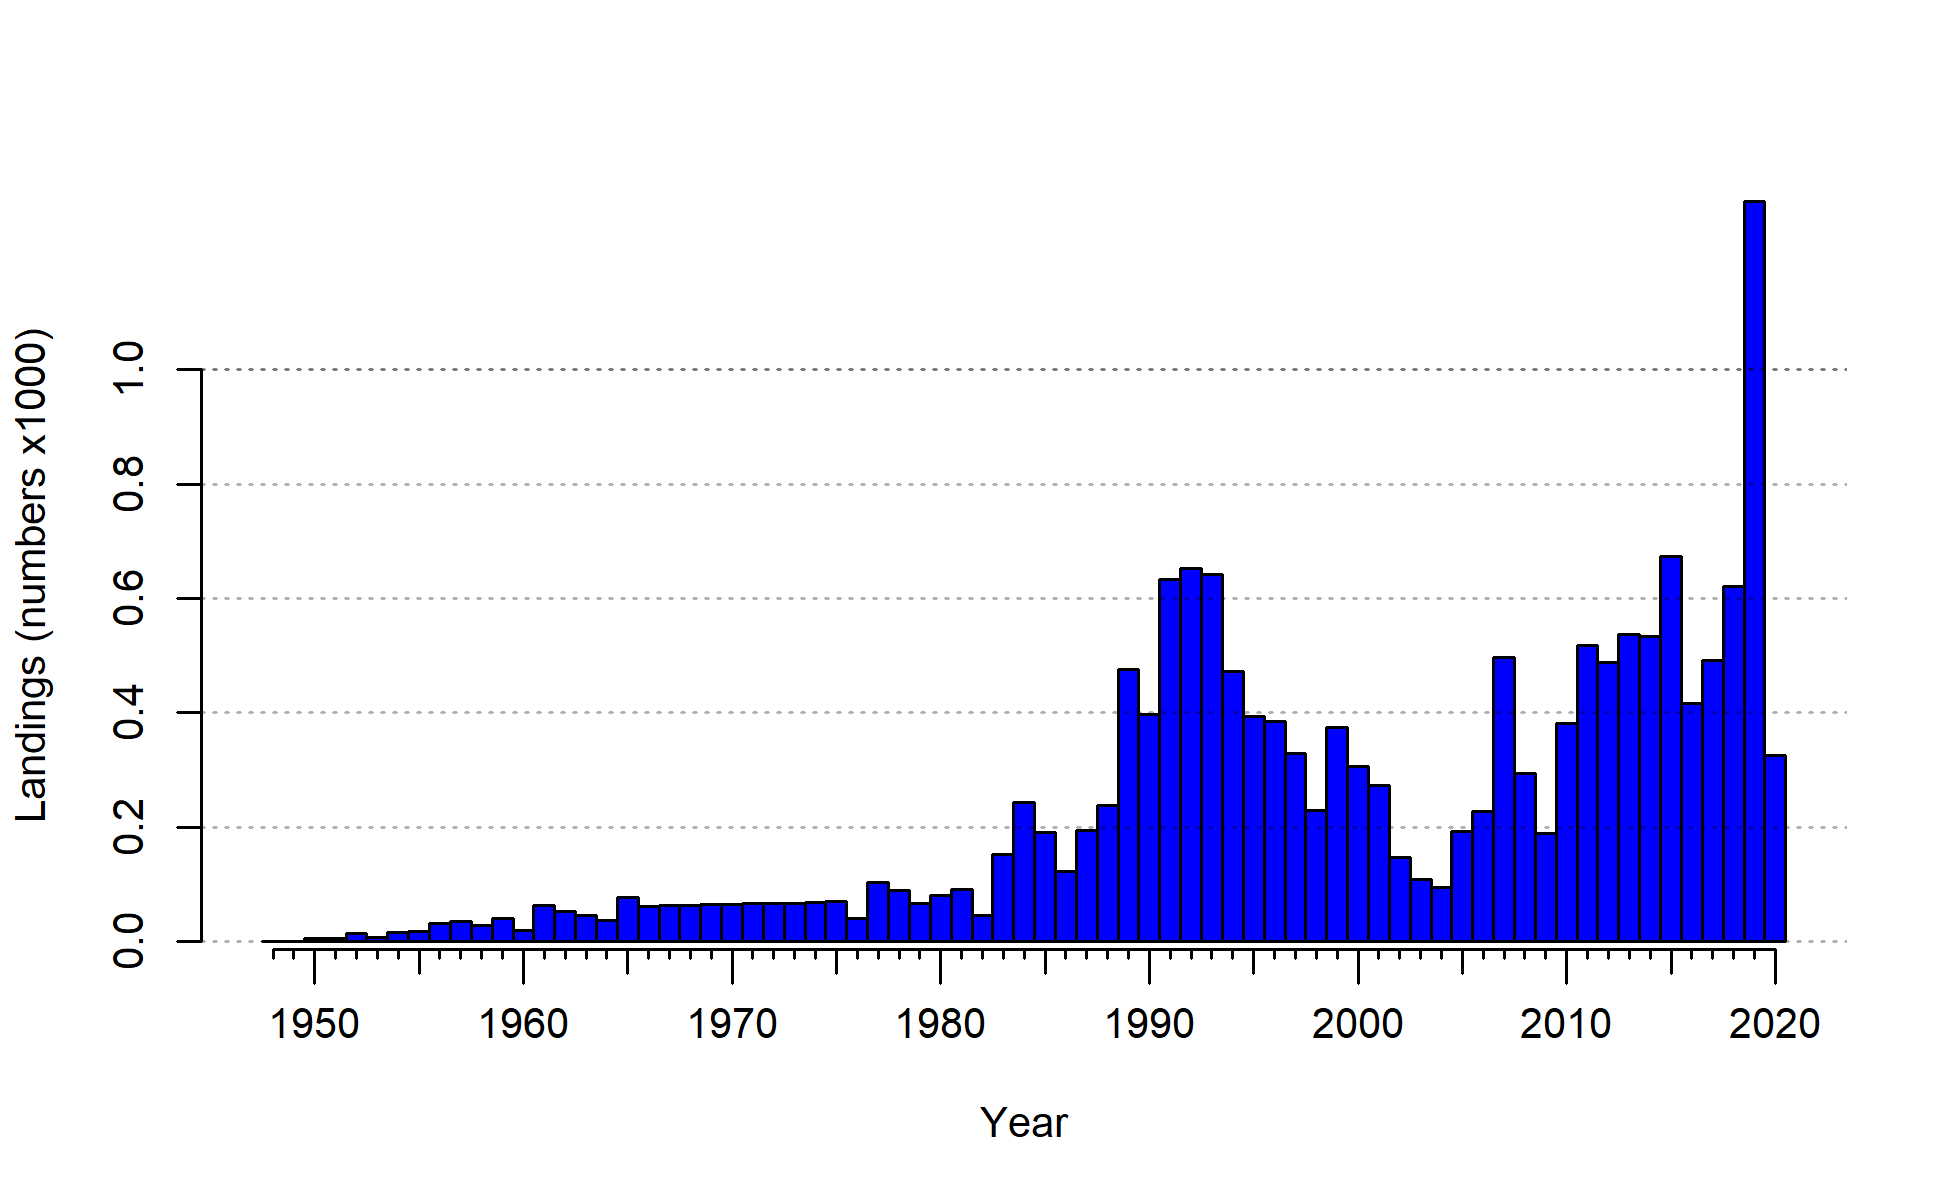
\includegraphics[width=1\textwidth,height=1\textheight]{C:/Users/Jason.Cope/Documents/Github/Vermilion rockfish OR WA assessment 2021/OR/write_up/models/Reference model/plots/catch2 landings stacked.png}
\caption{Landings by fleet used in the base model where catches in metric tons by fleet are stacked.\label{fig:es-catch}}
\end{figure}

\tagmcend\tagstructend

\clearpage

\tagstructbegin{tag=H2}\tagmcbegin{tag=H2}

\hypertarget{data-and-assessment}{%
\subsection*{Data and Assessment}\label{data-and-assessment}}
\addcontentsline{toc}{subsection}{Data and Assessment}

\leavevmode\tagmcend\tagstructend

\tagstructbegin{tag=P}\tagmcbegin{tag=P}

The stock assessment for vermilion rockfish off Oregon state was developed using the length- and age-structured model Stock Synthesis (version 3.30.16). No previous stock assessment for vermilion rockfish off Oregon has been conducted. Model structure included two fleets (commercial and recreational) and one fishery-based index of abundance. Life history parameters were sex-specific (i.e., a two-sex model) with natural mortality and growth parameters estimated, along with recruitment. The model time domain is 1892 to 2020, with a 12 year forecast beginning in 2021.

\leavevmode\tagmcend\tagstructend\par

\tagstructbegin{tag=P}\tagmcbegin{tag=P}

This assessment integrates data and information from multiple sources into one modeling framework. Specifically, the assessment uses landings data, length and conditional age-at-length composition data (using ageing error matrices to incorporate ageing imprecision) for each fishery, and one index of abundance based from the recreational fishery; fixed parameterizations of weight-at-length, maturity-at-length, and fecundity-at-length, the Beverton-Holt stock-recruitment steepness value and recruitment variability. Estimated values include initial population scale ({\tagstructbegin{tag=Formula}\tagmcbegin{tag=Formula}\(lnR_0\)\leavevmode\tagmcend\tagstructend}), natural mortality and growth for each sex, asymptotic selectivity and recruitment deviations. The base model was tuned to account for the weighting of the length and age data and index variances (which was estimated), as well as the specification of recruitment variance and recruitment bias adjustments. Derived quantities include the time series of spawning biomass, age and size structure, and current and projected future stock status.

\leavevmode\tagmcend\tagstructend\par

\tagstructbegin{tag=P}\tagmcbegin{tag=P}

Uncertainty is explicitly included in this assessment through variances of all estimated parameters, while between model uncertainty is explored through sensitivity analyses such as data treatment and weighting, and model specification sensitivity to the treatment of life history parameters, selectivity, and recruitment. A reference model was selected that best fit the observed data while concomitantly balancing the desire to capture the central tendency across those sources of uncertainty, ensure model realism and tractability, and promote robustness to potential model misspecification.

\leavevmode\tagmcend\tagstructend\par

\tagstructbegin{tag=H2}\tagmcbegin{tag=H2}

\hypertarget{stock-biomass}{%
\subsection*{Stock Biomass}\label{stock-biomass}}
\addcontentsline{toc}{subsection}{Stock Biomass}

\leavevmode\tagmcend\tagstructend

\tagstructbegin{tag=P}\tagmcbegin{tag=P}

Spawning output (in millions of eggs) instead of spawning biomass is used to report the mature population scale as fecundity is nonlinearly related to the weight of the population. The estimated spawning output at the beginning of 2021 was 21 mt (\textasciitilde95 percent asymptotic intervals: 10 to 33 mt, Table \ref{tab:ssbES} and Figure \ref{fig:es-ssb}), which when compared to unfished spawning biomass (29 mt) equates to a relative stock status level of 73 percent (\textasciitilde95 percent asymptotic intervals: 48 to 98 percent, Figure \ref{fig:es-depl}). Overall, spawning output declined with the onset of increasing commercial removals in the 1960s, continued to decline with the increase in recreational catches through the 1990s, even dropping below the target relative stock size. Major recruitment pulses since the mid 1990s onward that are supported by each of the data sets caused a sharp increase of the population through the mid 2010s, after which another decline. Minimum relative stock sizes of 34 percent of unfished levels were seen in 1995. Currently the stock is estimated to be well above the management target of {\tagstructbegin{tag=Formula}\tagmcbegin{tag=Formula}\(SB_{25\%}\)\leavevmode\tagmcend\tagstructend} in 2021 and has remained well above the target throughout the time series (Table \ref{tab:ssbES} and Figure \ref{fig:es-depl}).

\leavevmode\tagmcend\tagstructend\par

\begingroup\fontsize{10}{12}\selectfont
\begingroup\fontsize{10}{12}\selectfont

\begin{longtable}[t]{r>{\centering\arraybackslash}p{1.57cm}>{\centering\arraybackslash}p{1.57cm}>{\centering\arraybackslash}p{1.57cm}>{\centering\arraybackslash}p{1.57cm}>{\centering\arraybackslash}p{1.57cm}>{\centering\arraybackslash}p{1.57cm}}
\caption{\label{tab:ssbES}Estimated recent trend in spawning output and the fraction unfished and the 95 percent intervals.}\\
\toprule
Year & Spawning Output & Lower Interval & Upper Interval & Fraction Unfished & Lower Interval & Upper Interval\\
\midrule
\endfirsthead
\caption[]{Estimated recent trend in spawning output and the fraction unfished and the 95 percent intervals. \textit{(continued)}}\\
\toprule
Year & Spawning Output & Lower Interval & Upper Interval & Fraction Unfished & Lower Interval & Upper Interval\\
\midrule
\endhead

\endfoot
\bottomrule
\endlastfoot
2011 & 1.82 & -0.26 & 3.89 & 0.66 & 0.36 & 0.97\\
2012 & 1.82 & -0.30 & 3.94 & 0.66 & 0.34 & 0.99\\
2013 & 1.81 & -0.35 & 3.98 & 0.66 & 0.32 & 1.00\\
2014 & 1.81 & -0.41 & 4.02 & 0.66 & 0.30 & 1.02\\
2015 & 1.80 & -0.46 & 4.06 & 0.66 & 0.28 & 1.04\\
2016 & 1.77 & -0.54 & 4.08 & 0.64 & 0.24 & 1.05\\
2017 & 1.77 & -0.58 & 4.13 & 0.65 & 0.23 & 1.07\\
2018 & 1.76 & -0.64 & 4.15 & 0.64 & 0.20 & 1.08\\
2019 & 1.72 & -0.71 & 4.14 & 0.62 & 0.17 & 1.08\\
2020 & 1.56 & -0.88 & 3.99 & 0.57 & 0.07 & 1.07\\
2021 & 1.55 & -0.90 & 4.00 & 0.56 & 0.06 & 1.07\\*
\end{longtable}
\endgroup{}
\endgroup{}


\tagstructbegin{tag=Figure,alttext={Estimated time series of spawning output (circles and line: median; light broken lines: 95 percent intervals) for the base model.}}\tagmcbegin{tag=Figure}

\begin{figure}
\centering
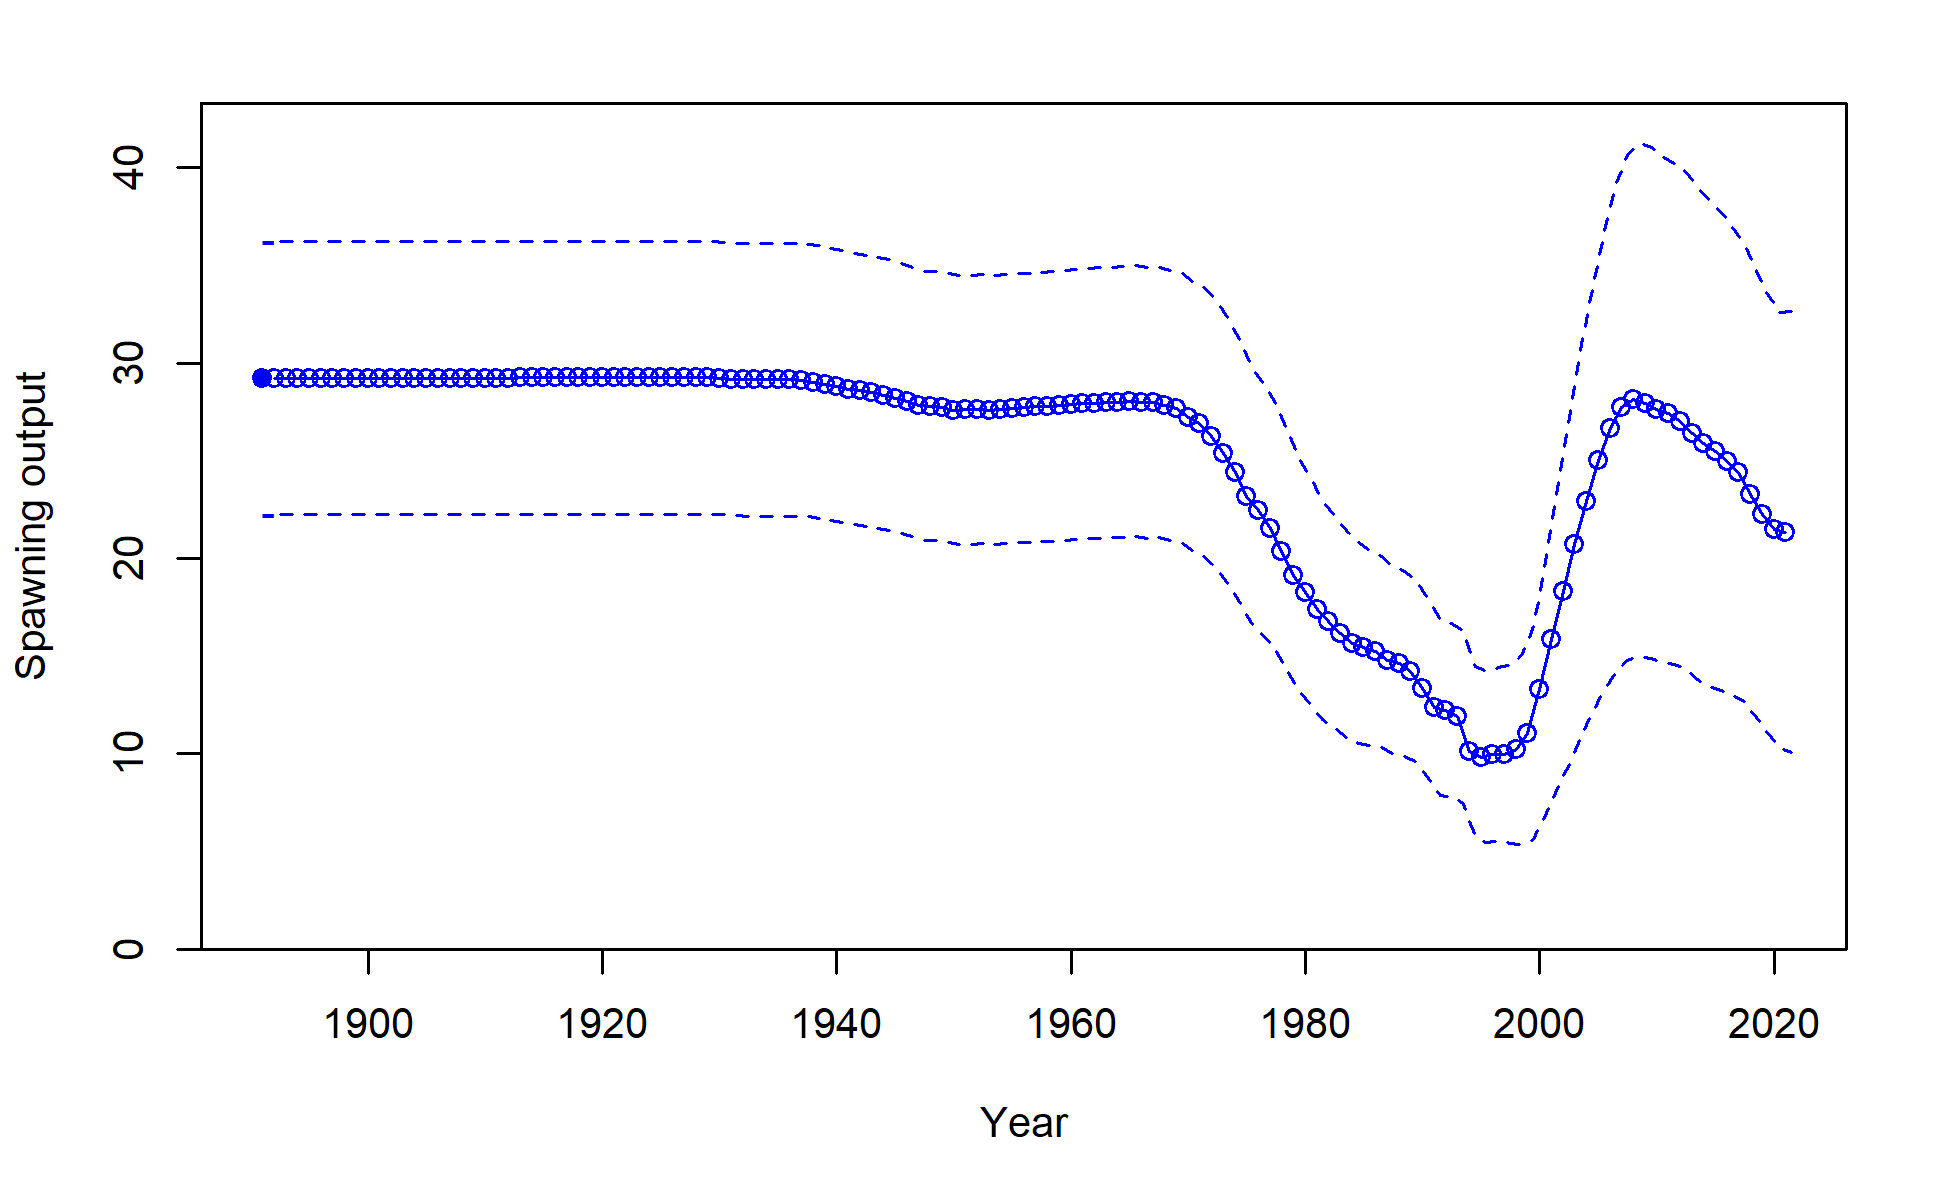
\includegraphics[width=1\textwidth,height=1\textheight]{C:/Users/Jason.Cope/Documents/Github/Vermilion rockfish OR WA assessment 2021/OR/write_up/models/Reference model/plots/ts7_Spawning_output_with_95_asymptotic_intervals_intervals.png}
\caption{Estimated time series of spawning output (circles and line: median; light broken lines: 95 percent intervals) for the base model.\label{fig:es-ssb}}
\end{figure}

\tagmcend\tagstructend

\tagstructbegin{tag=Figure,alttext={Estimated time series of fraction of unfished spawning output (circles and line: median; light broken lines: 95 percent intervals) for the base model.}}\tagmcbegin{tag=Figure}

\begin{figure}
\centering
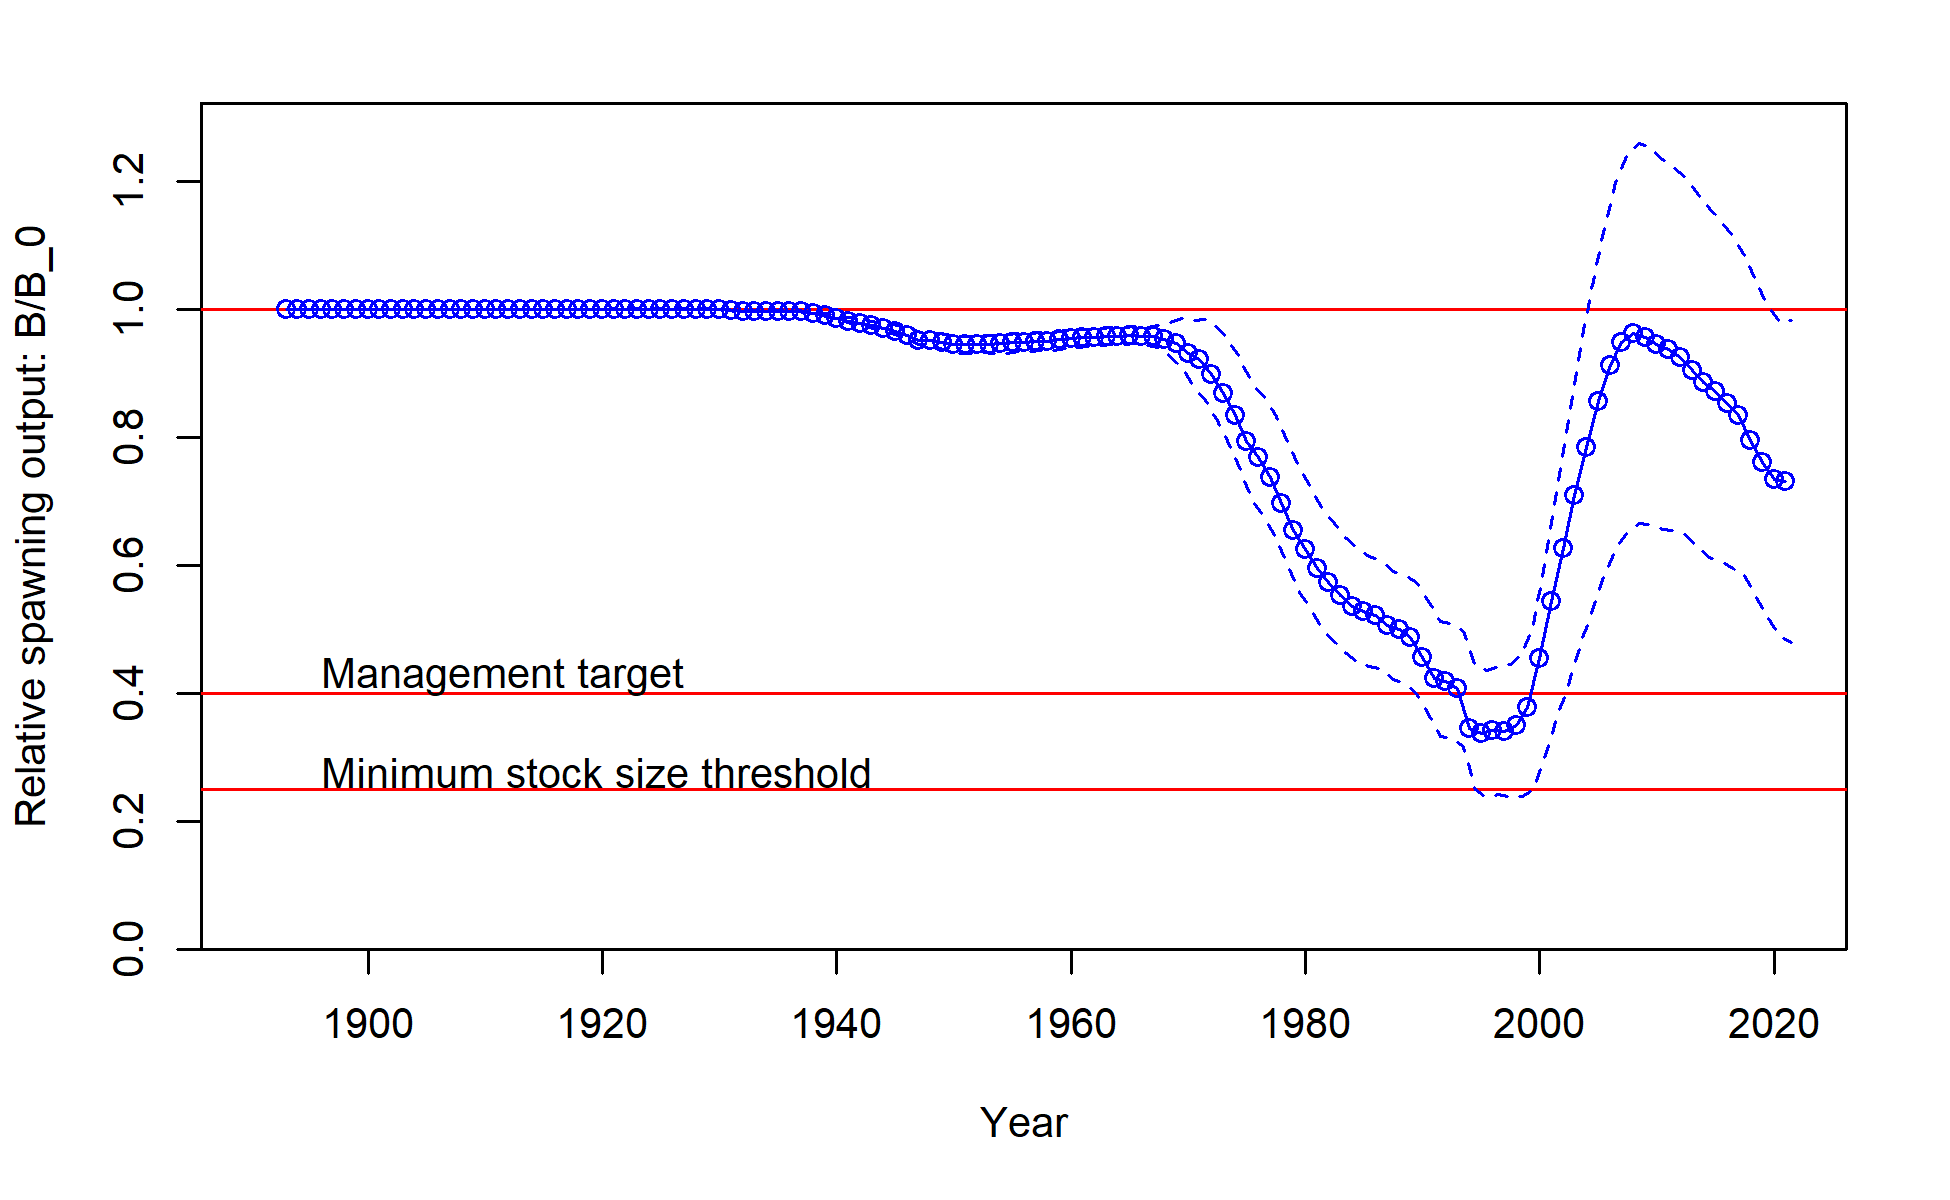
\includegraphics[width=1\textwidth,height=1\textheight]{C:/Users/Jason.Cope/Documents/Github/Vermilion rockfish OR WA assessment 2021/OR/write_up/models/Reference model/plots/ts9_Relative_spawning_output_intervals.png}
\caption{Estimated time series of fraction of unfished spawning output (circles and line: median; light broken lines: 95 percent intervals) for the base model.\label{fig:es-depl}}
\end{figure}

\tagmcend\tagstructend

\clearpage

\tagstructbegin{tag=H2}\tagmcbegin{tag=H2}

\hypertarget{recruitment}{%
\subsection*{Recruitment}\label{recruitment}}
\addcontentsline{toc}{subsection}{Recruitment}

\leavevmode\tagmcend\tagstructend

\tagstructbegin{tag=P}\tagmcbegin{tag=P}

Recruitment information begins in the 1960s and peaks in the 1990s (Table \ref{tab:recrES} and Figure \ref{fig:es-recruits}). Data were most informative from the the 1990s to the mid-2010s. Peaks years of recruitments are found in years 1993,1994, 1998, 2005 and 2015 (Figure \ref{fig:es-rec-devs}). Overall, the vermilion rockfish stock has not been reduced to levels that would provide considerable information on how recruitment changes with across spawning biomass levels (i.e., inform the steepness parameter). Thus, all recruitment is based on a fixed assumption about steepness ({\tagstructbegin{tag=Formula}\tagmcbegin{tag=Formula}\(h\)\leavevmode\tagmcend\tagstructend} = 0.72) and recruitment variability ({\tagstructbegin{tag=Formula}\tagmcbegin{tag=Formula}\(\sigma_R\)\leavevmode\tagmcend\tagstructend} = 0.6).

\leavevmode\tagmcend\tagstructend\par

\begingroup\fontsize{10}{12}\selectfont
\begingroup\fontsize{10}{12}\selectfont

\begin{longtable}[t]{r>{\centering\arraybackslash}p{1.57cm}>{\centering\arraybackslash}p{1.57cm}>{\centering\arraybackslash}p{1.57cm}>{\centering\arraybackslash}p{1.57cm}>{\centering\arraybackslash}p{1.57cm}>{\centering\arraybackslash}p{1.57cm}}
\caption{\label{tab:recrES}Estimated recent trend in recruitment (1000s of fish) and recruitment deviations and the 95 percent intervals.}\\
\toprule
Year & Recruitment & Lower Interval & Upper Interval & Recruitment Deviations & Lower Interval & Upper Interval\\
\midrule
\endfirsthead
\caption[]{Estimated recent trend in recruitment and recruitment deviations and the 95 percent intervals. \textit{(continued)}}\\
\toprule
Year & Recruitment & Lower Interval & Upper Interval & Recruitment Deviations & Lower Interval & Upper Interval\\
\midrule
\endhead

\endfoot
\bottomrule
\endlastfoot
2011 & 2.97 & 0.72 & 12.36 & 0.30 & -0.56 & 1.15\\
2012 & 1.77 & 0.42 & 7.56 & -0.23 & -1.20 & 0.74\\
2013 & 1.63 & 0.38 & 6.93 & -0.33 & -1.32 & 0.66\\
2014 & 1.81 & 0.42 & 7.77 & -0.24 & -1.28 & 0.81\\
2015 & 1.94 & 0.45 & 8.47 & -0.18 & -1.28 & 0.92\\
2016 & 2.24 & 0.50 & 9.95 & -0.04 & -1.19 & 1.10\\
2017 & 2.35 & 0.53 & 10.53 & -0.01 & -1.17 & 1.16\\
2018 & 2.35 & 0.52 & 10.56 & -0.01 & -1.17 & 1.16\\
2019 & 2.35 & 0.52 & 10.56 & -0.01 & -1.17 & 1.16\\
2020 & 2.32 & 0.51 & 10.55 & -0.01 & -1.17 & 1.16\\
2021 & 2.33 & 0.51 & 10.55 & 0.00 & -1.18 & 1.18\\*
\end{longtable}
\endgroup{}
\endgroup{}


\tagstructbegin{tag=Figure,alttext={Estimated time series of age-0 recruits (1000s) for the base model with 95 percent intervals.}}\tagmcbegin{tag=Figure}

\begin{figure}
\centering
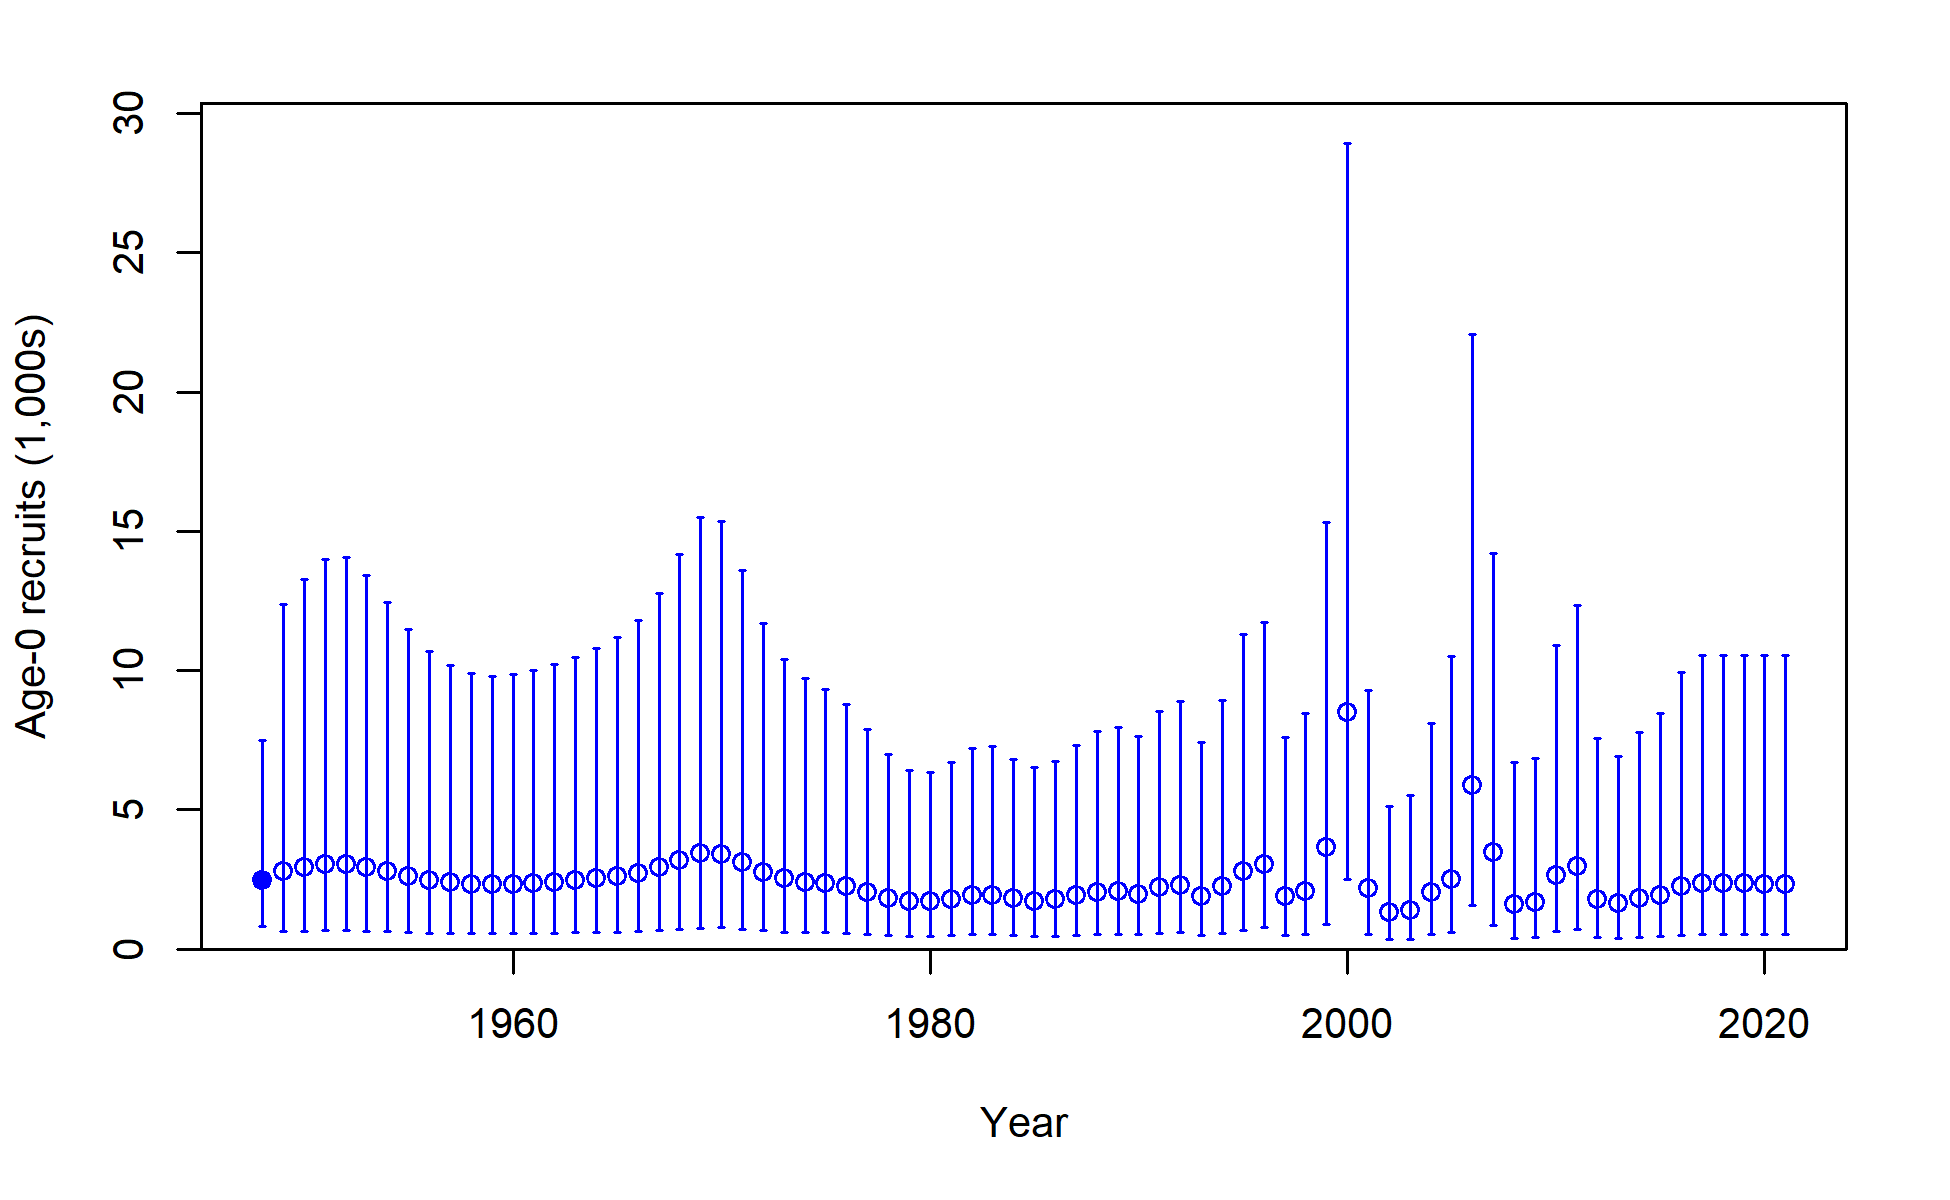
\includegraphics[width=1\textwidth,height=1\textheight]{C:/Users/Jason.Cope/Documents/Github/Vermilion rockfish OR WA assessment 2021/OR/write_up/models/Reference model/plots/ts11_Age-0_recruits_(1000s)_with_95_asymptotic_intervals.png}
\caption{Estimated time series of age-0 recruits (1000s) for the base model with 95 percent intervals.\label{fig:es-recruits}}
\end{figure}

\tagmcend\tagstructend

\tagstructbegin{tag=Figure,alttext={Estimated time series of recruitment deviations.}}\tagmcbegin{tag=Figure}

\begin{figure}
\centering
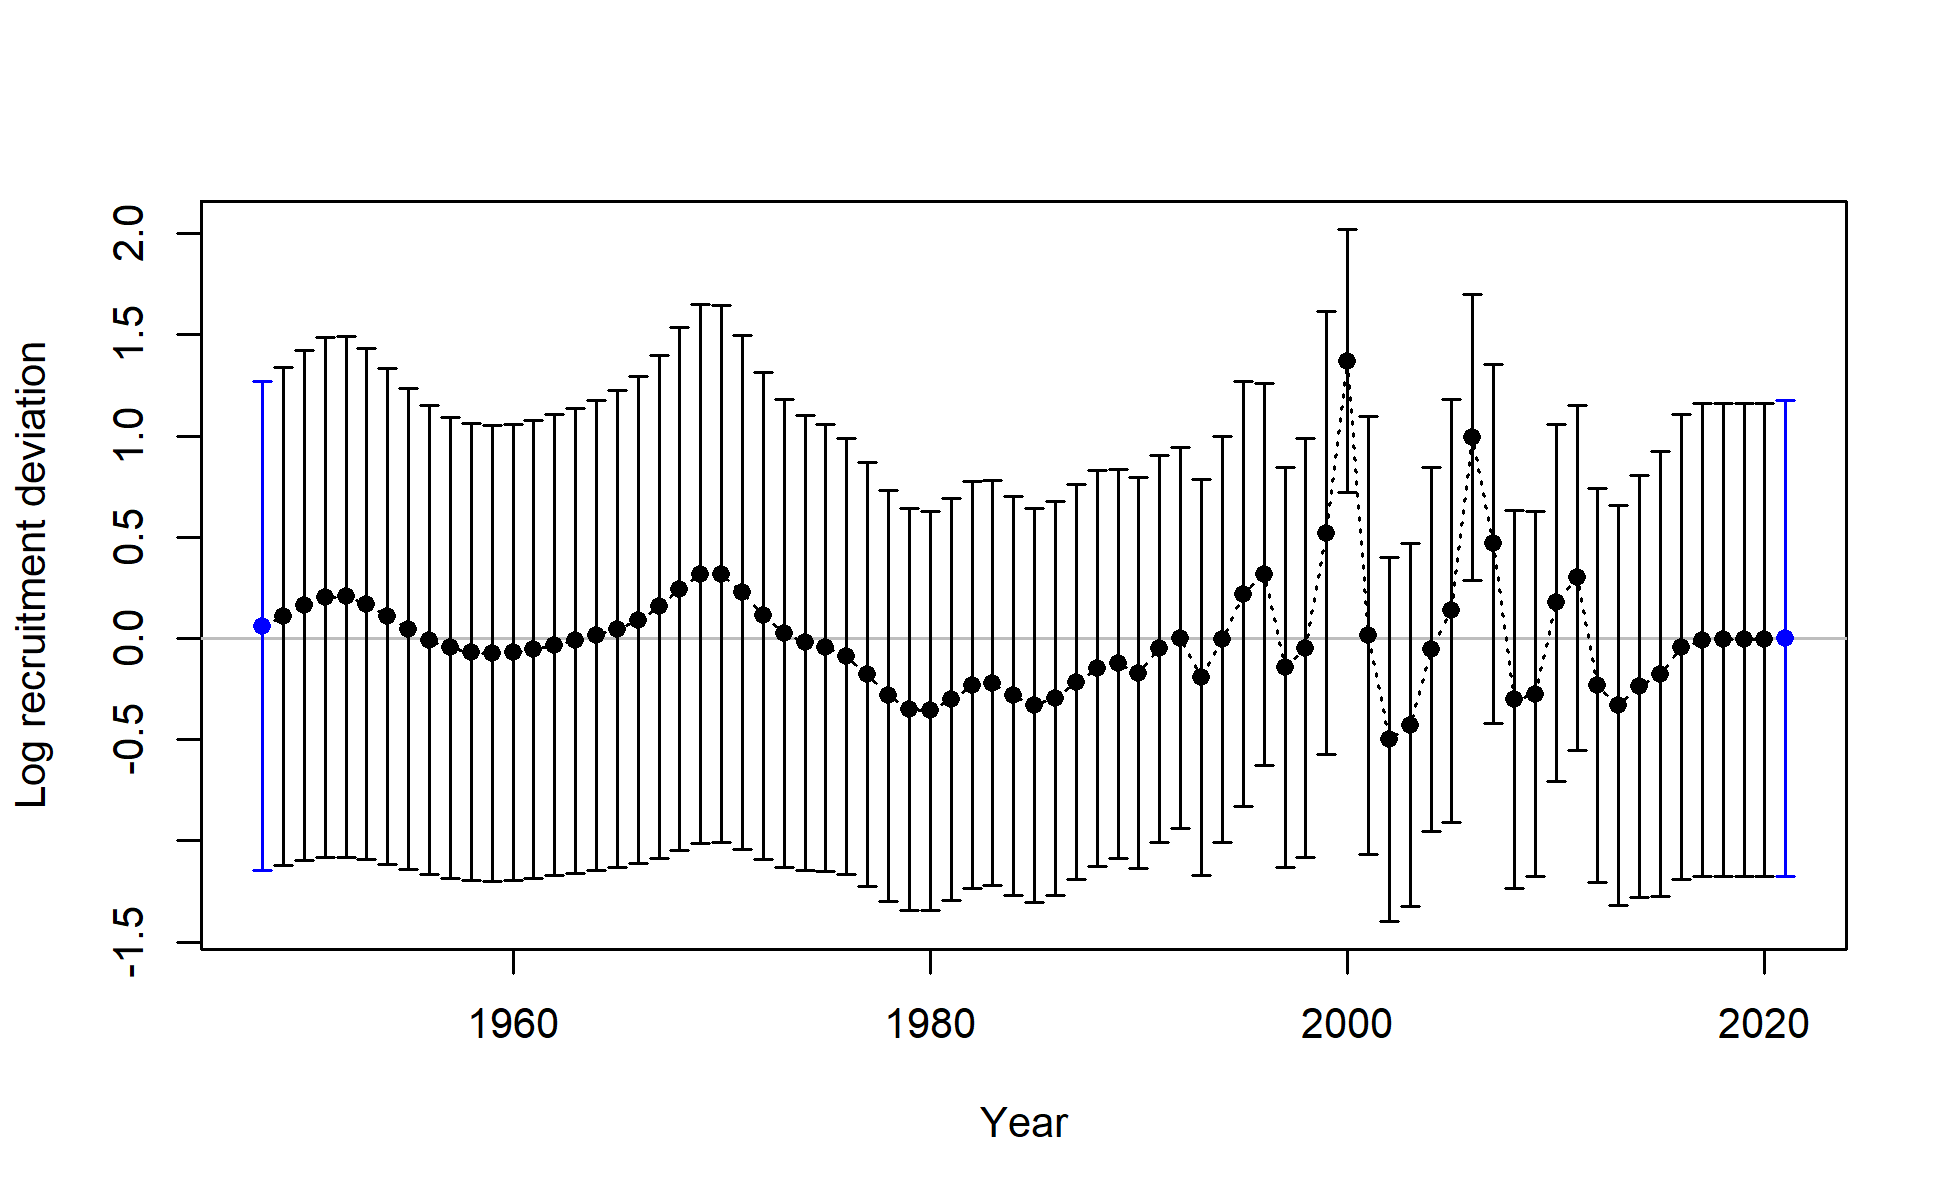
\includegraphics[width=1\textwidth,height=1\textheight]{C:/Users/Jason.Cope/Documents/Github/Vermilion rockfish OR WA assessment 2021/OR/write_up/models/Reference model/plots/recdevs2_withbars.png}
\caption{Estimated time series of recruitment deviations.\label{fig:es-rec-devs}}
\end{figure}

\tagmcend\tagstructend

\clearpage

\tagstructbegin{tag=H2}\tagmcbegin{tag=H2}

\hypertarget{exploitation-status}{%
\subsection*{Exploitation Status}\label{exploitation-status}}
\addcontentsline{toc}{subsection}{Exploitation Status}

\leavevmode\tagmcend\tagstructend

\tagstructbegin{tag=P}\tagmcbegin{tag=P}

Trends in fishing intensity (1 - SPR) largely mirrored that of landings until the 1990s when recruitment pulses overcame the catches to lower overall fishing intensity (Figure \ref{fig:es-1-spr}). The maximum fishing intensity was 0.84 in 1993, above the target SPR-based harvest rate of 0.50 (1 - {\tagstructbegin{tag=Formula}\tagmcbegin{tag=Formula}\(\text{SPR}_{50\%}\)\leavevmode\tagmcend\tagstructend}). Current levels of 0.47 for 2020 are near the fishing limit. Fishing intensity over the past decade has ranged between 0.27 and 0.51 and the exploitation rate has been high (0.02 - 0.05, Table \ref{tab:exploitES}). Current estimates indicate that vermilion rockfish spawning output is much greater than than the target biomass level ({\tagstructbegin{tag=Formula}\tagmcbegin{tag=Formula}\(\text{SB}_{40\%}\)\leavevmode\tagmcend\tagstructend}), though fishing intensity remains near target {\tagstructbegin{tag=Formula}\tagmcbegin{tag=Formula}\(F_MSY\)\leavevmode\tagmcend\tagstructend} proxy harvest rate.

\leavevmode\tagmcend\tagstructend\par

\begingroup\fontsize{10}{12}\selectfont
\begingroup\fontsize{10}{12}\selectfont

\begin{longtable}[t]{r>{\centering\arraybackslash}p{1.57cm}>{\centering\arraybackslash}p{1.57cm}>{\centering\arraybackslash}p{1.57cm}>{\centering\arraybackslash}p{1.57cm}>{\centering\arraybackslash}p{1.57cm}>{\centering\arraybackslash}p{1.57cm}}
\caption{\label{tab:exploitES}Estimated recent trend in the 1-SPR where SPR is the spawning potential ratio the exploitation rate, and the  95 percent intervals.}\\
\toprule
Year & 1-SPR & Lower Interval & Upper Interval & Fill in F method & Lower Interval & Upper Interval\\
\midrule
\endfirsthead
\caption[]{Estimated recent trend in the 1-SPR where SPR is the spawning potential ratio the exploitation rate, and the  95 percent intervals. \textit{(continued)}}\\
\toprule
Year & 1-SPR & Lower Interval & Upper Interval & Fill in F method & Lower Interval & Upper Interval\\
\midrule
\endhead

\endfoot
\bottomrule
\endlastfoot
2011 & 0.35 & 0.20 & 0.50 & 0.03 & 0.02 & 0.04\\
2012 & 0.43 & 0.26 & 0.59 & 0.04 & 0.02 & 0.06\\
2013 & 0.38 & 0.22 & 0.53 & 0.03 & 0.02 & 0.05\\
2014 & 0.28 & 0.15 & 0.41 & 0.02 & 0.01 & 0.03\\
2015 & 0.28 & 0.15 & 0.41 & 0.02 & 0.01 & 0.03\\
2016 & 0.27 & 0.15 & 0.40 & 0.02 & 0.01 & 0.03\\
2017 & 0.47 & 0.30 & 0.63 & 0.05 & 0.02 & 0.07\\
2018 & 0.48 & 0.31 & 0.65 & 0.05 & 0.03 & 0.07\\
2019 & 0.51 & 0.33 & 0.69 & 0.05 & 0.03 & 0.08\\
2020 & 0.47 & 0.29 & 0.64 & 0.05 & 0.02 & 0.07\\*
\end{longtable}
\endgroup{}
\endgroup{}


\tagstructbegin{tag=Figure,alttext={Estimated 1 - relative spawning ratio (SPR) by year for the base model. The management target is plotted as a red horizontal line and values above this reflect harvest in excess of the proxy harvest rate.}}\tagmcbegin{tag=Figure}

\begin{figure}
\centering
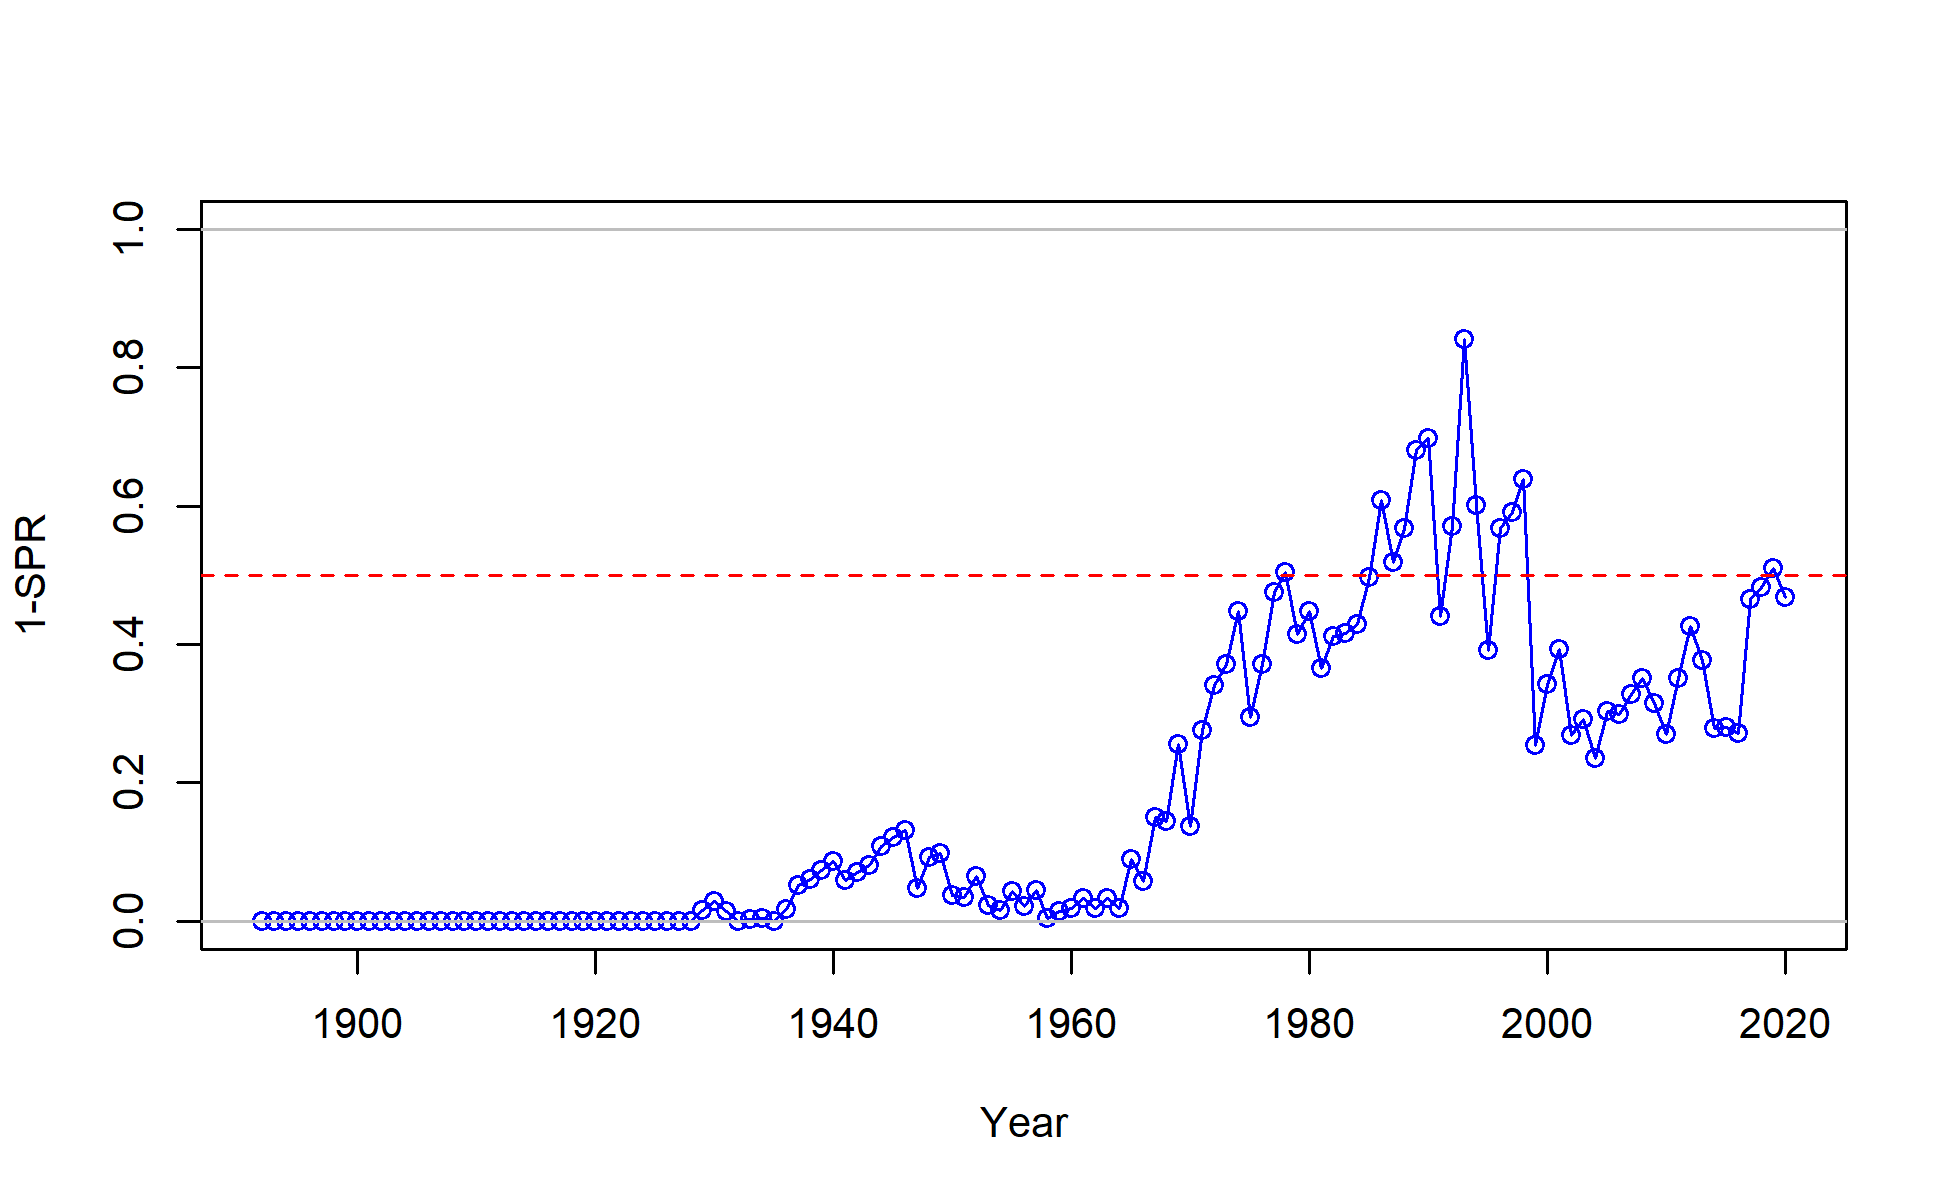
\includegraphics[width=1\textwidth,height=1\textheight]{C:/Users/Jason.Cope/Documents/Github/Vermilion rockfish OR WA assessment 2021/OR/write_up/models/Reference model/plots/SPR2_minusSPRseries.png}
\caption{Estimated 1 - relative spawning ratio (SPR) by year for the base model. The management target is plotted as a red horizontal line and values above this reflect harvest in excess of the proxy harvest rate.\label{fig:es-1-spr}}
\end{figure}

\tagmcend\tagstructend

\clearpage

\tagstructbegin{tag=H2}\tagmcbegin{tag=H2}

\hypertarget{ecosystem-considerations}{%
\subsection*{Ecosystem Considerations}\label{ecosystem-considerations}}
\addcontentsline{toc}{subsection}{Ecosystem Considerations}

\leavevmode\tagmcend\tagstructend

\tagstructbegin{tag=P}\tagmcbegin{tag=P}

No ecosystem considerations are included in this stock assessment.

\leavevmode\tagmcend\tagstructend\par

\tagstructbegin{tag=H2}\tagmcbegin{tag=H2}

\hypertarget{reference-points}\)\leavevmode\tagmcend\tagstructend}) across all model years are shown in Figure \ref{fig:es-phase} where warmer colors (red) represent early years and colder colors (blue) represent recent years. There have been periods where the stock status has decreased below the target and fishing intensity has been higher than the target fishing intensity based on {\tagstructbegin{tag=Formula}\tagmcbegin{tag=Formula}\(\text{SPR}_{50\%}\)\leavevmode\tagmcend\tagstructend}. Figure \ref{fig:es-yield} shows the equilibrium curve based on a steepness value fixed at 0.72 with vertical dashed lines to indicate the estimate of fraction unfished at the start of 2021 (current) and the estimated management targets calculated based on the relative target biomass (B target), the SPR target, and the maximum sustainable yield (MSY).

\leavevmode\tagmcend\tagstructend\par

\tagstructbegin{tag=Figure,alttext={Phase plot of estimated 1-SPR versus fraction unfished for the base model.}}\tagmcbegin{tag=Figure}

\begin{figure}
\centering
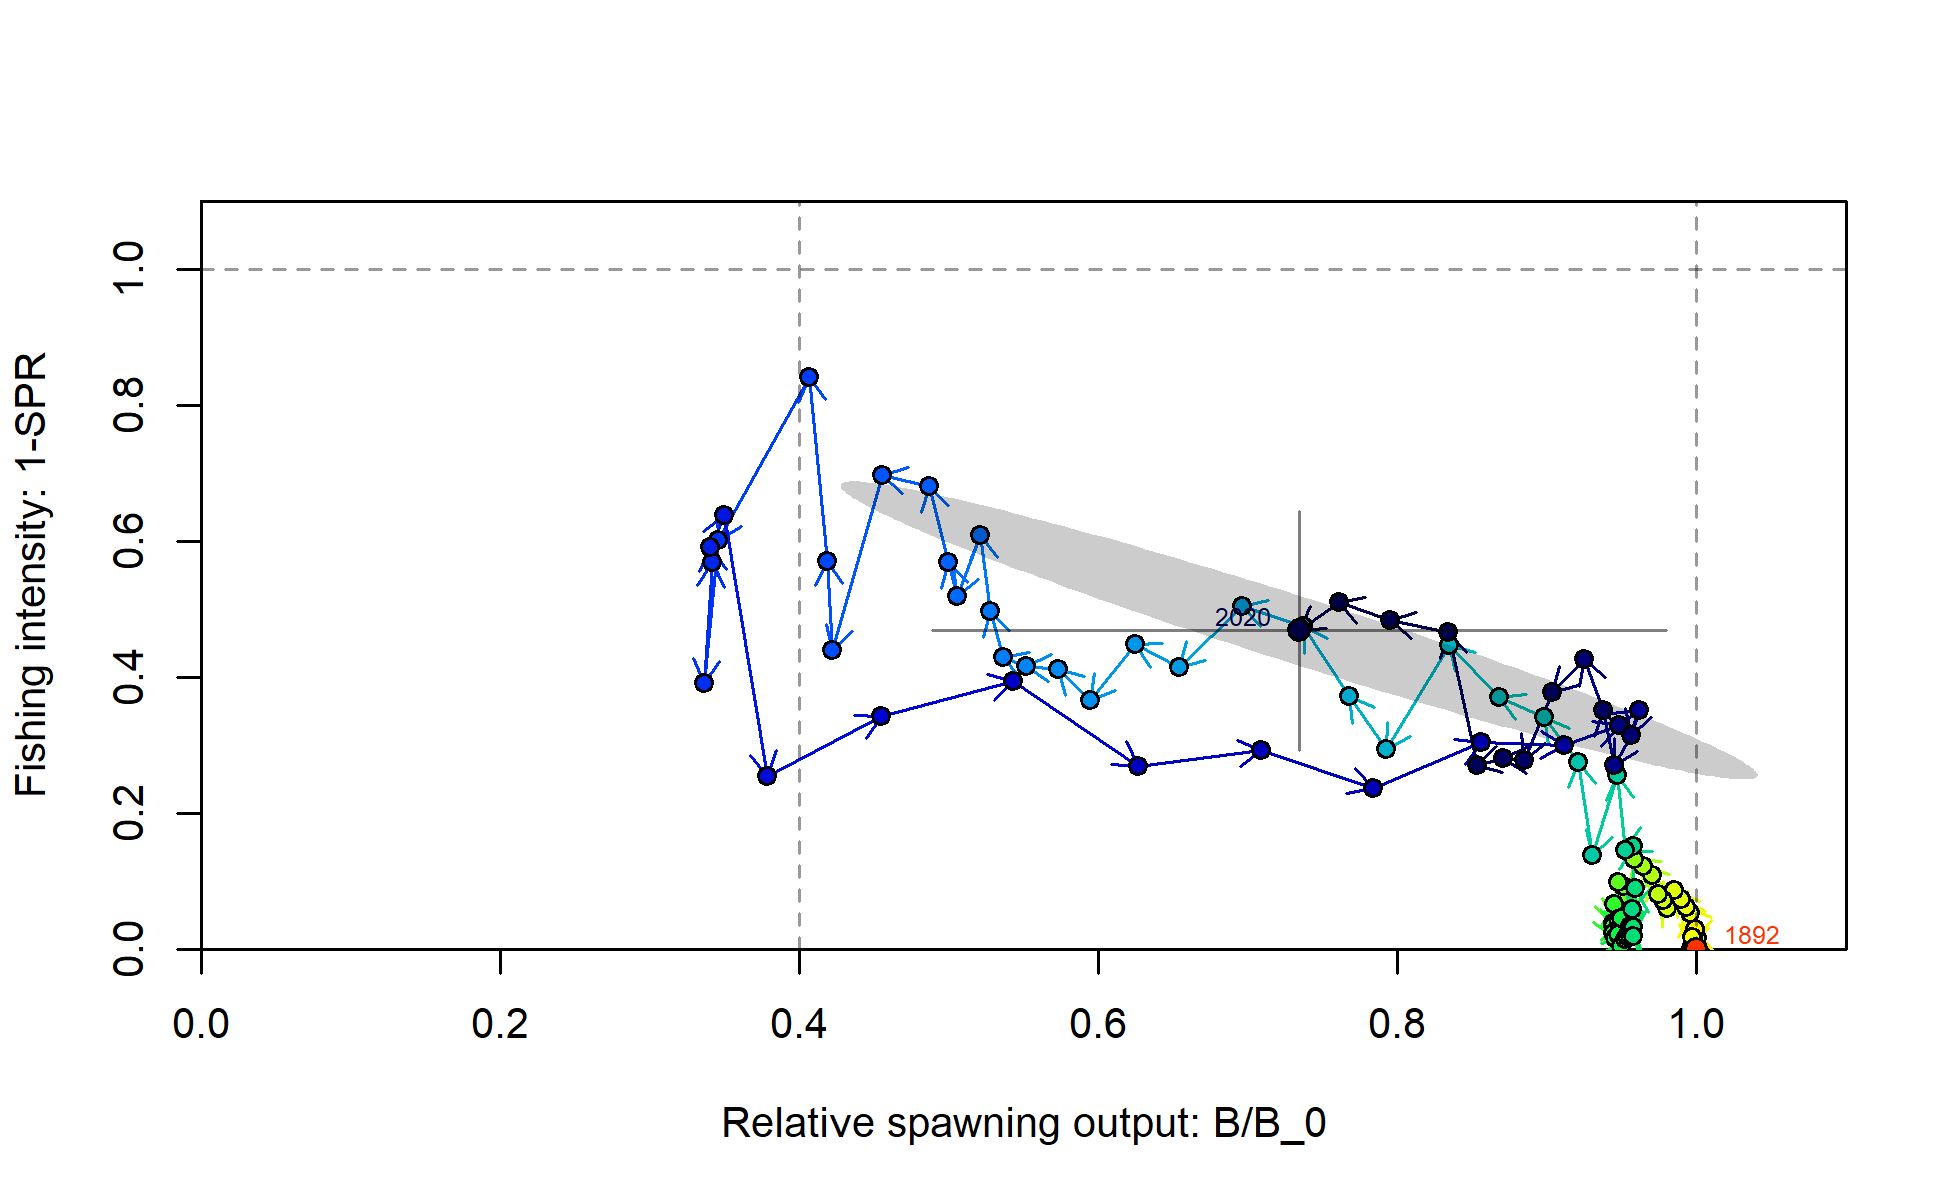
\includegraphics[width=1\textwidth,height=1\textheight]{C:/Users/Jason.Cope/Documents/Github/Vermilion rockfish OR WA assessment 2021/OR/write_up/models/Reference model/plots/SPR4_phase.png}
\caption{Phase plot of estimated 1-SPR versus fraction unfished for the base model.\label{fig:es-phase}}
\end{figure}

\tagmcend\tagstructend

\tagstructbegin{tag=Figure,alttext={Equilibrium yield curve for the base case model. Values are based on the 2020 fishery selectivities and with steepness fixed at 0.80.}}\tagmcbegin{tag=Figure}

\begin{figure}
\centering
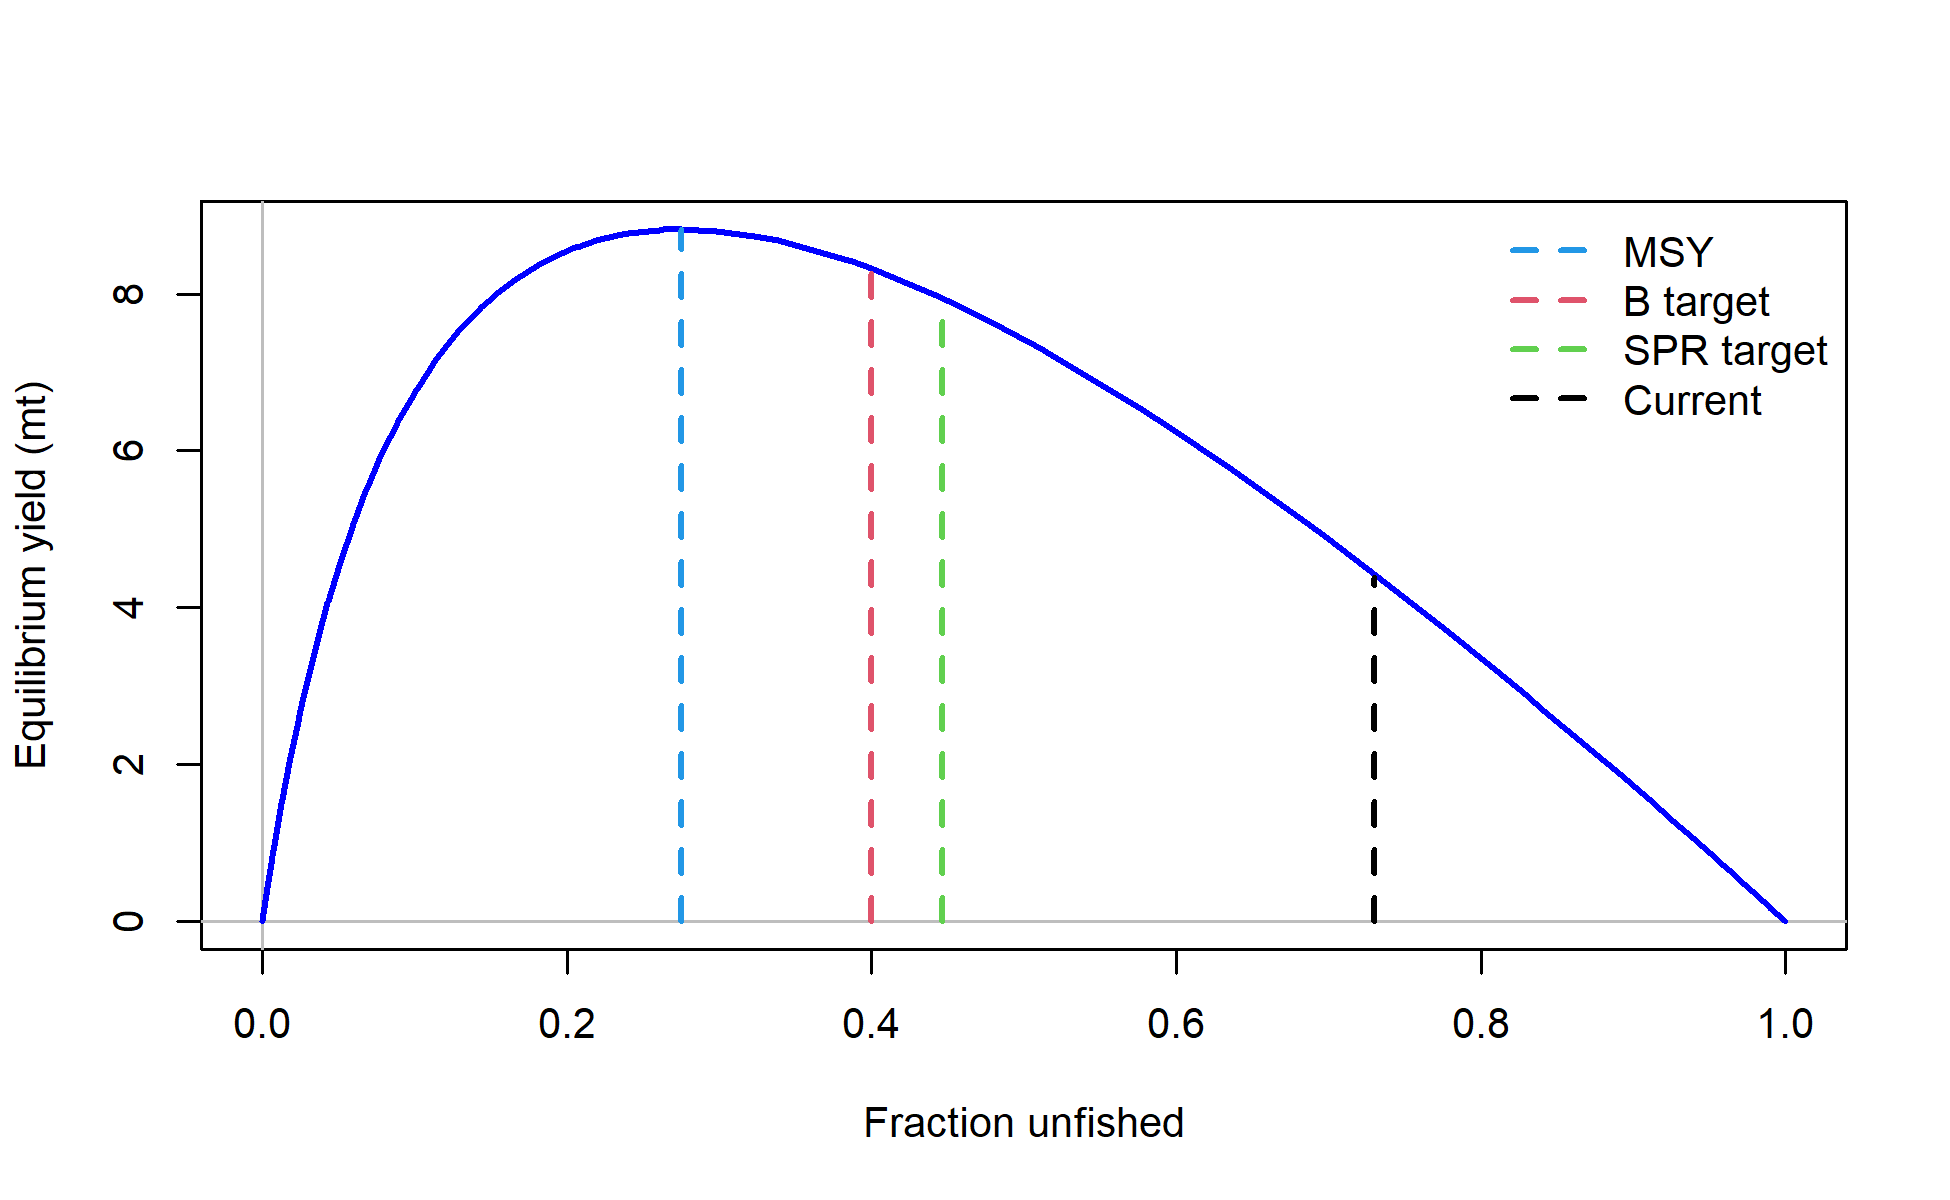
\includegraphics[width=1\textwidth,height=1\textheight]{C:/Users/Jason.Cope/Documents/Github/Vermilion rockfish OR WA assessment 2021/OR/write_up/models/Reference model/plots/yield2_yield_curve_with_refpoints.png}
\caption{Equilibrium yield curve for the base case model. Values are based on the 2020 fishery selectivities and with steepness fixed at 0.80.\label{fig:es-yield}}
\end{figure}

\tagmcend\tagstructend

\tagstructbegin{tag=P}\tagmcbegin{tag=P}

Reference points were calculated using the estimated selectivities and catch distributions among fleets in the most recent year of the model, 2020 (Table \ref{tab:es-reference}). Sustainable total yield, removals, using an {\tagstructbegin{tag=Formula}\tagmcbegin{tag=Formula}\(\text{SPR}_{50\%}\)\leavevmode\tagmcend\tagstructend} is 8 mt. The spawning biomass equivalent to 40 percent of the unfished spawning biomass ({\tagstructbegin{tag=Formula}\tagmcbegin{tag=Formula}\(\text{SB}_{40\%}\)\leavevmode\tagmcend\tagstructend}) calculated using the SPR target ({\tagstructbegin{tag=Formula}\tagmcbegin{tag=Formula}\(\text{SPR}_{50\%}\)\leavevmode\tagmcend\tagstructend}) was 13 mt. Recent removals have been close to the point estimate of potential long-term yields calculated using an {\tagstructbegin{tag=Formula}\tagmcbegin{tag=Formula}\(\text{SPR}_{50\%}\)\leavevmode\tagmcend\tagstructend} reference point and the population size has been relatively decreasing toward the target over the past few years.

\leavevmode\tagmcend\tagstructend\par

\begingroup\fontsize{10}{12}\selectfont
\begingroup\fontsize{10}{12}\selectfont

\begin{longtable}[t]{r>{\centering\arraybackslash}p{2cm}>{\centering\arraybackslash}p{2cm}>{\centering\arraybackslash}p{2cm}}
\caption{\label{tab:referenceES}Summary of reference points and management quantities, including estimates of the  95 percent intervals.}\\
\toprule
 & Estimate & Lower Interval & Upper Interval\\
\midrule
\endfirsthead
\caption[]{Summary of reference points and management quantities, including estimates of the  95 percent intervals. \textit{(continued)}}\\
\toprule
 & Estimate & Lower Interval & Upper Interval\\
\midrule
\endhead

\endfoot
\bottomrule
\endlastfoot
Unfished Spawning Output & 29.24 & 22.19 & 36.29\\
Unfished Age 3+ Biomass (mt) & 354.37 & 278.67 & 430.07\\
Unfished Recruitment (R0) & 16.33 & 8.52 & 24.13\\
Spawning Output (2021) & 21.35 & 10.06 & 32.65\\
Fraction Unfished (2021) & 0.73 & 0.48 & 0.98\\
\underline{Reference Points Based SB40\%} &  &  & \\
Proxy Spawning Output SB40\% & 11.70 & 8.88 & 14.51\\
SPR Resulting in SB40\% & 0.46 & 0.46 & 0.46\\
Exploitation Rate Resulting in SB40\% & 0.06 & 0.05 & 0.07\\
Yield with SPR Based On SB40\% (mt) & 8.32 & 5.57 & 11.07\\
\underline{Reference Points Based on SPR Proxy for MSY} &  &  & \\
Proxy Spawning Output (SPR50) & 13.04 & 9.90 & 16.19\\
SPR50 & 0.50 & & \\
Exploitation Rate Corresponding to SPR50 & 0.05 & 0.04 & 0.06\\
Yield with SPR50 at SB SPR (mt) & 7.95 & 5.32 & 10.57\\
\underline{Reference Points Based on Estimated MSY Values} &  &  & \\
Spawning Output at MSY (SB MSY) & 8.04 & 6.28 & 9.81\\
SPR MSY & 0.35 & 0.34 & 0.35\\
Exploitation Rate Corresponding to SPR MSY & 0.09 & 0.07 & 0.11\\
MSY (mt) & 8.82 & 5.89 & 11.76\\*
\end{longtable}
\endgroup{}
\endgroup{}


\clearpage

\tagstructbegin{tag=H2}\tagmcbegin{tag=H2}

\hypertarget{management-performance}{%
\subsection*{Management Performance}\label{management-performance}}
\addcontentsline{toc}{subsection}{Management Performance}

\leavevmode\tagmcend\tagstructend

\tagstructbegin{tag=P}\tagmcbegin{tag=P}

Exploitation on vermilion rockfish increased starting around 1960 and reached a high in the early 1990s. Since that time, catch has mostly fluctuated between 5-10 mt, with some values above 10 mt, particularly in the last 4 years. The last ten years of the vermilion component acceptable biological catch (ABC) and annual catch limit (ACL) (which are equivalent) of the Minor Shelf Rockfish North Complex has been set below the overfishing limit (OFL) (Table \ref{tab:ofl-es}), all of which have been exceeded in the most recent 4 years.

\leavevmode\tagmcend\tagstructend\par

\begingroup\fontsize{10}{12}\selectfont
\begingroup\fontsize{10}{12}\selectfont

\tagstructbegin{tag=Table}\tagmcbegin{tag=Table}
\begin{longtable}[t]{l>{\raggedright\arraybackslash}p{1.83cm}>{\raggedright\arraybackslash}p{1.83cm}>{\raggedright\arraybackslash}p{1.83cm}>{\raggedright\arraybackslash}p{1.83cm}>{\raggedright\arraybackslash}p{1.83cm}}
\caption{\label{tab:ofl-es}The OFL, ABC, ACL, landings, and the estimated total mortality in metric tons.}\\
\toprule
Year & OFL & ABC & ACL & Landings & Est. Total Mortality\\
\midrule
\endfirsthead
\caption[]{\label{tab:ofl-es}The OFL, ABC, ACL, landings, and the estimated total mortality in metric tons. \textit{(continued)}}\\
\toprule
Year & OFL & ABC & ACL & Landings & Est. Total Mortality\\
\midrule
\endhead

\endfoot
\bottomrule
\endlastfoot
2011 & 11.1 & 5.6 & 5.6 & 9 & 9\\
2012 & 11.1 & 5.6 & 5.6 & 12 & 12\\
2013 & 9.7 & 8.1 & 8.1 & 10 & 10\\
2014 & 9.7 & 8.1 & 8.1 & 6 & 6\\
2015 & 9.7 & 8.1 & 8.1 & 6 & 6\\
2016 & 9.7 & 8.1 & 8.1 & 6 & 6\\
2017 & 9.7 & 8.1 & 8.1 & 12 & 12\\
2018 & 9.7 & 8.1 & 8.1 & 12 & 12\\
2019 & 9.7 & 8.1 & 8.1 & 13 & 13\\
2020 & 9.7 & 8.1 & 8.1 & 11 & 11\\*
\end{longtable}
\leavevmode\tagmcend\tagstructend\par
\endgroup{}
\endgroup{}

\tagstructbegin{tag=H2}\tagmcbegin{tag=H2}

\hypertarget{unresolved-problems-and-major-uncertainties}{%
\subsection*{Unresolved Problems and Major Uncertainties}\label{unresolved-problems-and-major-uncertainties}}
\addcontentsline{toc}{subsection}{Unresolved Problems and Major Uncertainties}

\leavevmode\tagmcend\tagstructend

\tagstructbegin{tag=P}\tagmcbegin{tag=P}

The base case model was developed with the goal of balancing parsimony with realism and fitting the data. To achieve parsimony, some simplification of model structure was assumed which may impact the interpretation and fit to specific data sets. While life history values are estimated, uncertainty in natural mortality and growth parameters translates into uncertain estimates of both status and sustainable fishing levels for vermilion rockfish.

\leavevmode\tagmcend\tagstructend\par

\tagstructbegin{tag=H2}\tagmcbegin{tag=H2}

\hypertarget{scientific-uncertainty}{%
\subsection*{Scientific Uncertainty}\label{scientific-uncertainty}}
\addcontentsline{toc}{subsection}{Scientific Uncertainty}

\leavevmode\tagmcend\tagstructend

\tagstructbegin{tag=P}\tagmcbegin{tag=P}

The model estimated uncertainty around the 2021 spawning biomass was {\tagstructbegin{tag=Formula}\tagmcbegin{tag=Formula}\(\sigma\)\leavevmode\tagmcend\tagstructend} = 0.27 and the uncertainty around the OFL was {\tagstructbegin{tag=Formula}\tagmcbegin{tag=Formula}\(\sigma\)\leavevmode\tagmcend\tagstructend} = 0.31. This is likely an underestimate of overall uncertainty because of the necessity to fix some parameters such as steepness and no explicit incorporation of model structural uncertainty.

\leavevmode\tagmcend\tagstructend\par

\tagstructbegin{tag=H2}\tagmcbegin{tag=H2}

\hypertarget{harvest-projections-and-decision-table}{%
\subsection*{Harvest Projections and Decision Table}\label{harvest-projections-and-decision-table}}
\addcontentsline{toc}{subsection}{Harvest Projections and Decision Table}

\leavevmode\tagmcend\tagstructend

\tagstructbegin{tag=P}\tagmcbegin{tag=P}

TBD

\leavevmode\tagmcend\tagstructend\par

\tagstructbegin{tag=H2}\tagmcbegin{tag=H2}

\hypertarget{research-and-data-needs}{%
\subsection*{Research and Data Needs}\label{research-and-data-needs}}
\addcontentsline{toc}{subsection}{Research and Data Needs}

\leavevmode\tagmcend\tagstructend

\tagstructbegin{tag=P}\tagmcbegin{tag=P}

TBD

\leavevmode\tagmcend\tagstructend\par

\pagebreak
\setlength{\parskip}{5mm plus1mm minus1mm}
\pagenumbering{arabic}
\setcounter{page}{1}
\renewcommand{\thefigure}{\arabic{figure}}
\renewcommand{\thetable}{\arabic{table}}
\setcounter{table}{0}
\setcounter{figure}{0}

\setlength\parskip{0.5em plus 0.1em minus 0.2em}

\tagstructbegin{tag=H1}\tagmcbegin{tag=H1}

\hypertarget{introduction}{%
\section{Introduction}\label{introduction}}

\leavevmode\tagmcend\tagstructend

\tagstructbegin{tag=H2}\tagmcbegin{tag=H2}

\hypertarget{basic-information}{%
\subsection{Basic Information}\label{basic-information}}

\leavevmode\tagmcend\tagstructend

\tagstructbegin{tag=P}\tagmcbegin{tag=P}

This assessment reports the status of vermilion rockfish (\emph{Sebastes miniatus}) off the waters of Oregon state using data through 2020. Vermilion rockfish range from Prince William Sound, Alaska, to central Baja California at depths of 6 m to 436 m {\tagstructbegin{tag=Reference}\tagmcbegin{tag=Reference}(Love, Yoklavich, and Thorsteinson 2002)\leavevmode\tagmcend\tagstructend}. They are most commonly found from southern Oregon to Punta Baja, Mexico {\tagstructbegin{tag=Reference}\tagmcbegin{tag=Reference}(Hyde and Vetter 2009)\leavevmode\tagmcend\tagstructend} at depths of 50 m to 150 m {\tagstructbegin{tag=Reference}\tagmcbegin{tag=Reference}(Hyde and Vetter 2009)\leavevmode\tagmcend\tagstructend}. Hyde and Vetter {\tagstructbegin{tag=Reference}\tagmcbegin{tag=Reference}(2009)\leavevmode\tagmcend\tagstructend} describe an additional cryptic species related to vermilion rockfish, the sunset rockfish (\emph{Sebastes crocotulus}). They note that Vermilion rockfish are residents of shallower depths (\textless100 m) versus sunset rockfish. Sunset rockfish tend to be more southerly, and are not commonly encountered in Oregon, so this assessment focuses only on vermilion rockfish. Adult fish tend to cluster on high relief rocky outcrops {\tagstructbegin{tag=Reference}\tagmcbegin{tag=Reference}(Love, Yoklavich, and Thorsteinson 2002)\leavevmode\tagmcend\tagstructend} and kelp forests {\tagstructbegin{tag=Reference}\tagmcbegin{tag=Reference}(Hyde and Vetter 2009)\leavevmode\tagmcend\tagstructend}. North of Point Conception, some adults are shallower, living in caves and cracks {\tagstructbegin{tag=Reference}\tagmcbegin{tag=Reference}(Love, Yoklavich, and Thorsteinson 2002)\leavevmode\tagmcend\tagstructend}. Vermilion rockfish have shown high site fidelity {\tagstructbegin{tag=Reference}\tagmcbegin{tag=Reference}(Robert W. Hannah and Rankin 2011 (only tagged 1 vermilion); Lea, McAllister, and VenTresca 1999)\leavevmode\tagmcend\tagstructend}, and low average larval dispersal distance {\tagstructbegin{tag=Reference}\tagmcbegin{tag=Reference}(Hyde and Vetter 2009)\leavevmode\tagmcend\tagstructend}. Lowe et al. {\tagstructbegin{tag=Reference}\tagmcbegin{tag=Reference}(\textbf{Lowe2009?})\leavevmode\tagmcend\tagstructend} suggested vermilion rockfish to have a lower site fidelity than previously believed, but they acknowledged that their observations of movements to different depths may have been due to the reality of a shallower species and a deeper species.

\leavevmode\tagmcend\tagstructend\par

\tagstructbegin{tag=P}\tagmcbegin{tag=P}

The stock designation of Oregon waters was based on the California stock having a separate explotation history as well as a much larger stock density. Vermilion rockfish are not as abundant north of Califoria, but still provide some fishing opportunities {\tagstructbegin{tag=Reference}\tagmcbegin{tag=Reference}(Robert W. Hannah and Kautzi 2012)\leavevmode\tagmcend\tagstructend}. The separation of Oregon and Washington into distinct mangement units, and thus separate stock assessments, were based on the observation that most vermilion in Oregon are taken off southern Oregon, while most of the habitat and take of vermilion off Washington was in the very northern portion of the Washington coast (Figure \ref{fig:ORWA-map}). Ninty percent of the total mortality in Oregon is from the southern part of the state (south of Pt. Arago), while ninty-seven percent comes from the northern portion of Washington (Figure \ref{fig:tm-plot}). This large area separation, low movement of larvae and adults, and the biogeographic barriers of the Columbia River outfall and lack of rocky habitat in southern Washington all support separate Oregon-Washington management units.

\leavevmode\tagmcend\tagstructend\par

\tagstructbegin{tag=H2}\tagmcbegin{tag=H2}

\hypertarget{life-history}{%
\subsection{Life History}\label{life-history}}

\leavevmode\tagmcend\tagstructend

\tagstructbegin{tag=P}\tagmcbegin{tag=P}

Approximate lifespan for vermilion rockfish is 60 years, with females living longer and growing larger than their male counterparts. 50\% are mature at 5 years and about 37 cm, with males probably maturing at shorter lengths than females {\tagstructbegin{tag=Reference}\tagmcbegin{tag=Reference}(Love, Yoklavich, and Thorsteinson 2002)\leavevmode\tagmcend\tagstructend}.

\leavevmode\tagmcend\tagstructend\par

\tagstructbegin{tag=P}\tagmcbegin{tag=P}

Vermilion rockfish are viviparous, and release 63,000 to 2,600,000 eggs per season. In southern California, vermilion rockfish larvae are released between July and March. In central and northern California, this release occurs in September, December, and April-June {\tagstructbegin{tag=Reference}\tagmcbegin{tag=Reference}(Love, Yoklavich, and Thorsteinson 2002)\leavevmode\tagmcend\tagstructend}. In Oregon, fertilized females with ripe ovaries are encountered from April to Ocotber {\tagstructbegin{tag=Reference}\tagmcbegin{tag=Reference}(Robert W. Hannah and Kautzi 2012)\leavevmode\tagmcend\tagstructend}, with larval release sometime during and after that period. Larval release in fall and winter is not common among other rockfish species. Hyde and Vetter {\tagstructbegin{tag=Reference}\tagmcbegin{tag=Reference}(2009)\leavevmode\tagmcend\tagstructend} suggest that low larval dispersal may be due to weak poleward flow of nearshore waters corresponding with peak vermilion larval release.

\leavevmode\tagmcend\tagstructend\par

\tagstructbegin{tag=P}\tagmcbegin{tag=P}

Young-of-the-year (YOY) vermilion rockfish settle out of the plankton during two recruitment periods per year, first from February to April and a second from August to October, and settlement has been observed in May off southern California {\tagstructbegin{tag=Reference}\tagmcbegin{tag=Reference}(Love, Yoklavich, and Thorsteinson 2002)\leavevmode\tagmcend\tagstructend}. There is no information on YOY settlement in Oregon. Larvae measure about 4.3 mm. Both young-of-the-year vermilion and sunset rockfish are mottled brown with areas of black, and older juveniles turn a mottled orange or red color {\tagstructbegin{tag=Reference}\tagmcbegin{tag=Reference}(Love et al. 2012)\leavevmode\tagmcend\tagstructend}. Juvenile fish are found individually from 6 m to 36 m, living near sand and structures. After two months, juveniles travel deeper and live on low relief rocky outcrops and other structures {\tagstructbegin{tag=Reference}\tagmcbegin{tag=Reference}(Love, Yoklavich, and Thorsteinson 2002)\leavevmode\tagmcend\tagstructend}.

\leavevmode\tagmcend\tagstructend\par

\tagstructbegin{tag=P}\tagmcbegin{tag=P}

Adult vermilion rockfish predominantly eat smaller fish, though sometimes they pursue euphausiids and other various macroplankton {\tagstructbegin{tag=Reference}\tagmcbegin{tag=Reference}(Phillips 1964)\leavevmode\tagmcend\tagstructend}. Love {\tagstructbegin{tag=Reference}\tagmcbegin{tag=Reference}(2002)\leavevmode\tagmcend\tagstructend} noted their diet to include octopus, salps, shrimps, and pelagic red crabs.

\leavevmode\tagmcend\tagstructend\par

\tagstructbegin{tag=H2}\tagmcbegin{tag=H2}

\hypertarget{ecosystem-considerations-1}{%
\subsection{Ecosystem Considerations}\label{ecosystem-considerations-1}}

\leavevmode\tagmcend\tagstructend

\tagstructbegin{tag=P}\tagmcbegin{tag=P}

This stock assessment does not explicitly incorporate trophic interactions, habitat factors (other than as inform relative abundance indices) or environmental factors into the assessment model, but a brief description of likely or potential ecosystem considerations are provided below.

\leavevmode\tagmcend\tagstructend\par

\tagstructbegin{tag=P}\tagmcbegin{tag=P}

Vermilion/sunset rockfish are described as feeding on a wide range of both pelagic and benthic prey items, including forage fish species such as anchovies and mesopelagic fishes, squid, krill and octopus, as well as sporadically abundant pelagic organisms such as pyrosomes, salps and pelagic red crabs {\tagstructbegin{tag=Reference}\tagmcbegin{tag=Reference}(Phillips 1964; \textbf{Love2002?})\leavevmode\tagmcend\tagstructend}. Interestingly, other rockfishes (either juvenile or adult stages) have not been documented as prey for vermilion, as they have been for other larger \emph{Sebastes} species such as cowcod, bocaccio and yelloweye rockfish. For the latter species, the idea of ``cultivation effects,'' in which adults crop down forage species that are potential competitors/predators of their own juveniles {\tagstructbegin{tag=Reference}\tagmcbegin{tag=Reference}(\textbf{Walters2001?})\leavevmode\tagmcend\tagstructend}, have been suggested by {\tagstructbegin{tag=Reference}\tagmcbegin{tag=Reference}(\textbf{Baskett2006?})\leavevmode\tagmcend\tagstructend}. For example, Baskett et al. {\tagstructbegin{tag=Reference}\tagmcbegin{tag=Reference}(\textbf{Baskett2006?})\leavevmode\tagmcend\tagstructend} found that in such scenarios there could be alternative stable states in which either the overfished species or the smaller prey species could dominate. While the sparse diet data for vermilion/sunset rockfish do not suggest such a process for this species complex, food habits data for vermilion/sunset are not robust, and the larger community processes on these rocky reef communities may also influence productivity and community composition regardless of the direct predation interactions. Pelagic and benthic juvenile vermilion and sunset rockfish are likely preyed upon by the same wide range of predators that prey on juveniles and adults of other rockfish species, including seabirds, piscivorous fishes, and marine mammals.

\leavevmode\tagmcend\tagstructend\par

\tagstructbegin{tag=P}\tagmcbegin{tag=P}

As with most other rockfish and groundfish in the California Current, recruitment, or cohort (year-class) strength appears to be highly variable for the vermilion/sunset rockfish complex, with only a modest apparent relationship to spawning output. Oceanographic and ecosystem factors are widely recognized to be key drivers of recruitment variability for most species of groundfish, as well as most elements of California Current food webs. Empirical estimates of recruitment from pelagic juvenile rockfish surveys have been used to inform incoming year class strength for some of these stocks, however vermilion and sunset rockfish are rarely encountered in these surveys. Specifically, only 47 of nearly 300,000 total juvenile \emph{Sebastes} encountered in juvenile surveys since 2001 were identified as vermilion or sunset rockfish {\tagstructbegin{tag=Reference}\tagmcbegin{tag=Reference}(\textbf{Field2021?})\leavevmode\tagmcend\tagstructend}. Despite this, the results here suggest that at least a reasonable fraction of recruitment variability for sunset and vermilion rockfish is shared with other rockfish and groundfish stocks throughout the California Current, many of which also had strong year classes in 1984, 1999 and 2015. Previous studies have demonstrated that large-scale oceanographic drivers, such as the relative transport of subarctic waters (typically indicated by relative sea level) tend to relate to a substantial fraction of overall groundfish recruitment trends and ecosystem productivity {\tagstructbegin{tag=Reference}\tagmcbegin{tag=Reference}(\textbf{Schroeder2019?})\leavevmode\tagmcend\tagstructend}. Although it is feasible that ecosystem factors, the results of pre-recruit surveys for co-occurring species, or the results of other groundfish assessments might ultimately be used to forecast recruitment for more data-limited stocks such as vermilion/sunset, as suggested by {\tagstructbegin{tag=Reference}\tagmcbegin{tag=Reference}(\textbf{Thorson2014?})\leavevmode\tagmcend\tagstructend}, such approaches would require more development and evaluation. Consequently, environmental factors are not explicitly considered in this assessment.

\leavevmode\tagmcend\tagstructend\par

\tagstructbegin{tag=H2}\tagmcbegin{tag=H2}

\hypertarget{historical-and-current-fishery-information}{%
\subsection{Historical and Current Fishery Information}\label{historical-and-current-fishery-information}}

\leavevmode\tagmcend\tagstructend

\tagstructbegin{tag=P}\tagmcbegin{tag=P}

Off the coast of Oregon, vermilion rockfish is caught in both commercial and recreational fisheries. The landings from the commercial fishery were minimal until the mid-1960s. Following the development of the nearshore commercial fishery in the late 1990s, Oregon Department of Fish and Wildlife (ODFW) implemented a state-permitted limited access fishery that regulated fleet size, period landing limits and established harvest guidelines {\tagstructbegin{tag=Reference}\tagmcbegin{tag=Reference}(\textbf{rodomsky\_2019\_2020?})\leavevmode\tagmcend\tagstructend}. Vermilion rockfish is one of multiple rockfish species that are commonly landed as a part of the nearshore commercial groundfish fishery. Currently, this commercial fishery is centered on the southern Oregon coast, where most of the vermilion rockfish commercial landings occur. Two types of state limited entry permits are issued for this fishery, with and without a nearshore endorsement. Limited entry permit holders without a nearshore endorsement may land commercial quantities of black and blue rockfish under state trip limits, with an additional total of 15 lbs per day of any combination of other nearshore groundfish species and two rockfish species with Federal designation as shelf rockfish. These include tiger and vermilion rockfish. Vessels that have a nearshore endorsement permit may land commercial quantities of other nearshore groundfish species up to the state's cumulative trip limits and the Federal limits for tiger and vermilion rockfish. There are no state trip limits set for vermilion rockfish.

\leavevmode\tagmcend\tagstructend\par

\tagstructbegin{tag=P}\tagmcbegin{tag=P}

This analysis assesses the stock off the Oregon coast as a separate stock from other populations off the West Coast based on the sedentary nature of vermillion rockfish, which likely limits flow of fish between California and Washington. The substrate of the northern Oregon and southern Washington coast is primarily sandy bottom and combined with the Columbia River plume between Oregon and Washington these factors create a natural separation between the Oregon and Washington populations. Additionally, the exploitation history and magnitude of removals off the Oregon coast has been dramatically lower than removals off the California coast. The recreational fishery off the coast of Oregon developed during the 1970s, with the first recorded landings of vermillion rockfish in 1979. Vermilion rockfish is not commonly encountered in the recreational fishery, but recreational removals have generally increased across time as this fishery has developed (Table \ref{tab:allcatches}).

\leavevmode\tagmcend\tagstructend\par

\tagstructbegin{tag=H2}\tagmcbegin{tag=H2}

\hypertarget{summary-of-management-history-and-performance}{%
\subsection{Summary of Management History and Performance}\label{summary-of-management-history-and-performance}}

\leavevmode\tagmcend\tagstructend

\tagstructbegin{tag=P}\tagmcbegin{tag=P}

Vermilion rockfish is managed by the Pacific Fishery Management Council (PFMC) as a part of the Shelf Rockfish North and Shelf Rockfish South complexes. The North and South areas are split at N. 40°10' Lat. N. off the West Coast. The complex is managed based on a complex level overfishing limit (OFL) and annual catch limit (ACL). The OFL and ACL values for the complex are determined by summing the species specific OFLs and ACLs managed within the complex. Removals for species within the Rockfish complex are managed and tracked against the complex total OFL and ACL, rather than on a species by species basis. The OFL and ACLs for vermilion rockfish North of 40°10' Lat. N. management area and the total removals are shown in Table \ref{tab:OR_vermilion_mgmt}. There are no state-specific allocations of this complex and so removals are evaluated at the regional level (North of 40°10').

\leavevmode\tagmcend\tagstructend\par

\tagstructbegin{tag=H1}\tagmcbegin{tag=H1}

\hypertarget{data-and-model-inputs}{%
\section{Data and Model Inputs}\label{data-and-model-inputs}}

\leavevmode\tagmcend\tagstructend

\tagstructbegin{tag=P}\tagmcbegin{tag=P}

A description of each data source is provided below (Figure \ref{fig:data-plot}).

\leavevmode\tagmcend\tagstructend\par

\tagstructbegin{tag=H2}\tagmcbegin{tag=H2}

\hypertarget{fishery-dependent-data}{%
\subsection{Fishery-Dependent Data}\label{fishery-dependent-data}}

\leavevmode\tagmcend\tagstructend

\tagstructbegin{tag=H3}\tagmcbegin{tag=H3}

\hypertarget{commercial}{%
\subsubsection{Commercial}\label{commercial}}

\leavevmode\tagmcend\tagstructend

\tagstructbegin{tag=H4}\tagmcbegin{tag=H4}

\hypertarget{landings-1}{%
\paragraph{Landings}\label{landings-1}}

\leavevmode\tagmcend\tagstructend

\tagstructbegin{tag=P}\tagmcbegin{tag=P}

In Oregon, historical commercial landings from 1892 to 1986 were provided by ODFW (Karnowski et al.~2014). Historical landings were consistent but minimal (\textless{} 1 mt) until the mid-1960s, except for a period from the mid-1930s to the late 1940s, during which landings increased to a high of 2.8 mt and declined again to under one mt. From 1965 to 1986, landings averaged 6.6 mt annually. Primary gear types during this historical period included longline and troll gears. However, ODFW commercial samplers suggest that these troll landings were primarily landed on hook and line gear, but not separated by gear type on the fish tickets (pers. comm. M. Freeman, ODFW).

\leavevmode\tagmcend\tagstructend\par

\tagstructbegin{tag=P}\tagmcbegin{tag=P}

Landings from 1987 -- 1999 were compiled from a combination of PacFIN, the central repository for West coast commercial landings (extracted on 11/17/2020), and a separate ODFW reconstruction that delineated species-specific landings in the unspecified categories on PacFIN (e.g.~URCK and POP1, ODFW 2017). Vermilion rockfish landings from this reconstruction were substituted for the URCK and POP1 landings available from PacFIN, and added to PacFIN landings from other categories for a complete time series during this time period. Commercial landings from 2000 -- 2020 are available on PacFIN (extracted on 11/17/2020 and 02/18/2021). Vermilion rockfish is one of several rockfish species landed by a nearshore, primarily live-fish fixed gear fishery centered on Oregon's southern coast. Following the development of this nearshore commercial fishery in the late 1990s, ODFW implemented a state-permitted limited access fishery that regulated fleet size, period landing limits and established harvest guidelines (Rodomsky et al.~2020). Vermilion rockfish are landed almost exclusively with hook and line and bottom longline gear. On average, 99.8\% of vermilion rockfish landings are from these two gear types (2000 -- 2020). Landings from all other gear types, including fish pot and trawl, are minimal relative to jig and longline gears and sporadic. Commercial landings peaked in 1993 at 13.9 mt before declining and fluctuating between 1.5 and 4.8 mt (2000 -- 2020). Landings in 2020 were 3.3 mt. Table \ref{tab:allcatches} provides landings by fleet over time.

\leavevmode\tagmcend\tagstructend\par

\tagstructbegin{tag=H4}\tagmcbegin{tag=H4}

\hypertarget{lengths}{%
\paragraph{Lengths}\label{lengths}}

\leavevmode\tagmcend\tagstructend

\tagstructbegin{tag=P}\tagmcbegin{tag=P}

Commercial vermilion rockfish length samples are available from PacFIN from 1999 -- 2020 (n = 2,355). Table \ref{tab:OR_vermilion_lengthsamples} shows sample size by year and fleet and Figure \ref{fig:comm-rec-lts_bubbs} shows the length compositions across time. These samples were extracted on 02/24/2021. Approximately 47.9\% of these samples are females (n = 1,129) and 51.9\% are males (n = 1,222). Only four fish were unsexed. The majority (93.3\%) are from the southern Oregon coast, centered in Port Orford (67.4\%) and Gold Beach (25.8\%), where the majority of permit holders for the commercial nearshore fishery are based and where most of the landings are made. The majority of length samples are from vermilion rockfish landed to the fresh (dead) market (93.5\%). Additionally, special projects length samples collected from the commercial fishery are available from PacFIN from 2000 - 2006, 2008 - 2009, and 2012 (n = 381; extracted on 02/24/2021). Special projects samples were not included in the length compositions used in this model as they were not randomly sampled from the fishery.

\leavevmode\tagmcend\tagstructend\par

\tagstructbegin{tag=H4}\tagmcbegin{tag=H4}

\hypertarget{ages}{%
\paragraph{Ages}\label{ages}}

\leavevmode\tagmcend\tagstructend

\tagstructbegin{tag=P}\tagmcbegin{tag=P}

There were 896 commercial age samples available from 2004 and 2007 - 2020 (Table \ref{tab:OR_vermilion_agesamples}). Approximately, 50.1\% of samples were males (n = 449) and 49.9\% were females (n = 447). As with the length samples, the vast majority of samples are from the southern Oregon coast (95.8\%, n = 858), including Port Orford (73.4\%) and Gold Beach (22.3\%).

\leavevmode\tagmcend\tagstructend\par

\tagstructbegin{tag=H3}\tagmcbegin{tag=H3}

\hypertarget{recreational}{%
\subsubsection{Recreational}\label{recreational}}

\leavevmode\tagmcend\tagstructend

\tagstructbegin{tag=H4}\tagmcbegin{tag=H4}

\hypertarget{removals}{%
\paragraph{Removals}\label{removals}}

\leavevmode\tagmcend\tagstructend

\tagstructbegin{tag=P}\tagmcbegin{tag=P}

Recreational landings and estimated discards are available in Table \ref{tab:allcatches}.

\leavevmode\tagmcend\tagstructend\par

\tagstructbegin{tag=H5}\tagmcbegin{tag=H5}

\hypertarget{historic-ocean-boat-landings-1979-2000}{%
\subparagraph{Historic Ocean Boat Landings (1979 -- 2000)}\label{historic-ocean-boat-landings-1979-2000}}

\leavevmode\tagmcend\tagstructend

\tagstructbegin{tag=P}\tagmcbegin{tag=P}

Recently, the Oregon Department of Fish and Wildlife (ODFW) undertook an effort to comprehensively reconstruct all marine fish recreational ocean boat landings prior to 2001 (pers. comm. A. Whitman, ODFW). Reconstructed catch estimates from the Oregon Recreational Boat Survey (ORBS) improve upon estimates from the federal Marine Recreational Fisheries Statistical Survey (MRFSS), which have known biases related to effort estimation and sampling (Van Voorhees et al.~2000) that resulted in catch estimates considered implausible by ODFW. However, the ORBS sample estimates are known to lack the comprehensive spatial and temporal coverage of MRFSS. Addressing this coverage issue is a major part of this reconstruction. In general, the base data and methodology for these reconstructed estimates are consistent with recent assessments for other nearshore species (Dick et al.~2016; Dick et al.~2018; Haltuch et al.~2018; Cope et al.~2019).

\leavevmode\tagmcend\tagstructend\par

\tagstructbegin{tag=P}\tagmcbegin{tag=P}

Prior to 2001, ORBS monitored marine species in both multi-species categories, such as rockfish, flatfish, and other miscellaneous fishes, and as individual species, such as lingcod or halibut. For this comprehensive reconstruction, four species categories were selected to reconstruct, including rockfish, lingcod, flatfish and miscellaneous, which constitute the bulk of the managed marine fish species. Vermilion rockfish are a component of the rockfish species category.

\leavevmode\tagmcend\tagstructend\par

\tagstructbegin{tag=P}\tagmcbegin{tag=P}

Category-level estimates were expanded to account for gaps in sampling coverage in two separate pathways. First, estimates from five major ports were expanded to include unsampled winter months in years lacking complete coverage. Expansions were based on available year-round sampling data and excluded years where regulations may have impacted the temporal distribution of catch. Second, all other minor port estimates were expanded to include seasonal estimates in years lacking any sampling based on the amount of minor port catch as compared to all major port estimates. A subset of landings were sampled by ORBS for species compositions within these categories. Once category-level landings were comprehensive in space and time, species compositions were applied for the three multi-species categories, including rockfish, flatfish and miscellaneous fish. Borrowing rules for species compositions were specific to the category and determined based on a series of regression tree analyses that detailed the importance of each domain (year, month, port and fishing mode) to variability in compositions.

\leavevmode\tagmcend\tagstructend\par

\tagstructbegin{tag=P}\tagmcbegin{tag=P}

Ocean boat estimates from 1979 -- 2000 in numbers of fish of vermilion rockfish from the above described methods were converted to biomass using biological samples from MRFSS (pers. comm. A. Whitman, ODFW). MRFSS biological data are available from 1980 -- 1989 and 1993 -- 2000. An annual average weight was applied to the total annual number of fish to obtain an annual landings estimate. Several years missing biological data (1979, 1990 -- 1992) were filled in using neighboring years or interpolation. These landings in biomass were provided by ODFW and do not include an estimate of discards. In order to account for historical discards, 6\% was added to landings from 1979 -- 2000. This discard mortality estimate is an average of the annual discard mortality from 2001 -- 2020 available on RecFIN. Landings during this time period gradually increase to a peak of 13.0 mt in 1993 and fluctuate between four and six mt following that peak.

\leavevmode\tagmcend\tagstructend\par

\tagstructbegin{tag=H5}\tagmcbegin{tag=H5}

\hypertarget{modern-ocean-boat-landings-2001-2020}{%
\subparagraph{Modern Ocean Boat Landings (2001 -- 2020)}\label{modern-ocean-boat-landings-2001-2020}}

\leavevmode\tagmcend\tagstructend

\tagstructbegin{tag=P}\tagmcbegin{tag=P}

Recreational landings for ocean boat modes from 2001 -- 2020 are available from RecFIN. Both retained and released estimates of mortality are included, though retained mortality contributes the vast majority to total mortality. Release mortality is estimated from angler-reported release rates and the application of discard mortality rates from the PFMC. From 2001 -- 2020, landings averaged 5.8 mt, ranging from 3.2 to 9.3 mt. In 2020, ocean boat landings were 8.9 mt.

\leavevmode\tagmcend\tagstructend\par

\tagstructbegin{tag=H5}\tagmcbegin{tag=H5}

\hypertarget{shore-and-estuary-landings-1980-2020}{%
\subparagraph{Shore and Estuary Landings (1980 -- 2020)}\label{shore-and-estuary-landings-1980-2020}}

\leavevmode\tagmcend\tagstructend

\tagstructbegin{tag=P}\tagmcbegin{tag=P}

The ODFW does not currently sample shore and estuary boat fishing trips, and in recent assessments, ODFW has provided reconstructed species-specific estimates of shore and estuary landings from 1980 -- 2020 (Berger et al.~2015, Dick et al.~2018, Cope et al.~2019). When investigating shore and estuary data for this species, there were virtually no records of shore and estuary landings of vermilion rockfish, and so these were not included for this assessment.

\leavevmode\tagmcend\tagstructend\par

\tagstructbegin{tag=H4}\tagmcbegin{tag=H4}

\hypertarget{lengths-1}{%
\paragraph{Lengths}\label{lengths-1}}

\leavevmode\tagmcend\tagstructend

\tagstructbegin{tag=P}\tagmcbegin{tag=P}

Recreational length samples were obtained from three sources: MRFSS, RecFIN (ORBS) and ODFW special project sampling. Table \ref{tab:OR_vermilion_lengthsamples} details sample sizes by year and fleet. From 1980 -- 1989 and from 1993 -- 2000, the MRFSS program collected samples from ocean areas only (n = 403). ODFW provided MRFSS samples with the addition of a column that flagged length values imputed from weights to allow for selection of directly measured values. From 1980 -- 1989, total lengths (mm) were collected by MRFSS, which were converted to fork length. From 1993 -- 2000, fork length (mm) was collected. Only samples that were measured directly were used in the assessment model. These included samples from 1993 - 2000 only. Length samples from 2001 -- 2020 from the ORBS sampling program are available on RecFIN (n =11,081). All ORBS samples are by fork length (mm). All samples are from ocean trips. Special projects samples collected by ODFW staff from the recreational fishery are provided from 1998 -- 2001 (n = 54) but were not used in the length compositions for the assessment model.

\leavevmode\tagmcend\tagstructend\par

\tagstructbegin{tag=H4}\tagmcbegin{tag=H4}

\hypertarget{ages-1}{%
\paragraph{Ages}\label{ages-1}}

\leavevmode\tagmcend\tagstructend

\tagstructbegin{tag=P}\tagmcbegin{tag=P}

There were 1,180 recreational age samples available from 2005 -- 2020 (Table \ref{tab:OR_vermilion_agesamples}). Approximately, 46.0\% of samples were males (n = 543) and 53.7\% were females (n = 634). There were three unsexed samples (0.25\%). As with the length samples, the vast majority of samples are from the southern Oregon coast (80.6\%, n = 951), primarily from Charleston (24.0\%), Gold Beach (19.2\%), Bandon (18.2\%), and Brookings (18.1\%).

\leavevmode\tagmcend\tagstructend\par

\tagstructbegin{tag=H3}\tagmcbegin{tag=H3}

\hypertarget{index-of-abundance}{%
\subsubsection{Index of Abundance}\label{index-of-abundance}}

\leavevmode\tagmcend\tagstructend

\tagstructbegin{tag=H4}\tagmcbegin{tag=H4}

\hypertarget{oregon-orbs-dockside-index-2001-2020}{%
\paragraph{Oregon ORBS Dockside Index (2001-2020)}\label{oregon-orbs-dockside-index-2001-2020}}

\leavevmode\tagmcend\tagstructend

\tagstructbegin{tag=P}\tagmcbegin{tag=P}

Trip-level catch-per-unit-effort data from ORBS dockside sampling was obtained from ODFW on 04/15/2021. To mitigate the confounding of hourly effort associated with these trips with travel, the travel time was subtracted from the hours fished. Travel time was stratified by boat type (charter and private) and was calculated as boat type-specific speeds (13 mph for charter boat trips and 18 mph for private boat trips) multiplied by twice the distance between the port of origin and the reef that was fished. CPUE, expressed in terms of fish per angler-hour, was calculated by multiplying the number of anglers and the adjusted travel time. The database contains information on catch by species (number of retained fish), effort (angler hours), sample location (port where data were collected), date, bag limits, boat type (charter or private), and trip type (e.g., bottom associated fish).

\leavevmode\tagmcend\tagstructend\par

\tagstructbegin{tag=H5}\tagmcbegin{tag=H5}

\hypertarget{orbs-cpue-data-preparation-filtering-and-sample-sizes}{%
\subparagraph{ORBS CPUE Data Preparation, Filtering, and Sample Sizes}\label{orbs-cpue-data-preparation-filtering-and-sample-sizes}}

\leavevmode\tagmcend\tagstructend

\tagstructbegin{tag=P}\tagmcbegin{tag=P}

In order to define effective fishing effort for Vermilion (i.e.~identify trips that were likely to catch the species), the method of Stephens and MacCall {\tagstructbegin{tag=Reference}\tagmcbegin{tag=Reference}(\textbf{stephens\_multispecies\_2004?})\leavevmode\tagmcend\tagstructend} was used to predict the probability of catching a Vermilion given the occurrence of other species in the catch. The unfiltered data set contained 411,528 trips. Multiple standardized filters are applied to ORBS trip-level data in order to remove outliers and data unsuitable for an index. These filters include trips with incorrect interview times, which impact calculation of effort, unreasonably long or short trips, and retaining bottomfish target trips. There were 117,042 trips available for the application of the Stephens-MacCall filter (Table \ref{tab:ORBS_filter_criteria}). Species that are rarely encountered will provide little information about the likelihood of catching Vermilion, and so 47 ``indicator'' species that were caught in at least 30 Oregon trips (Figure \ref{fig:s-m-coef}) were used to predict vermilion catch. Catch of these commonly-encountered species in a given trip was coded as presence/absence (1/0) and treated as a categorical variable in the Stephens-MacCall logistic regression analysis.

\leavevmode\tagmcend\tagstructend\par

\tagstructbegin{tag=P}\tagmcbegin{tag=P}

The top six species with a high probability of co-occurrence with Vermilion include Other Rockfish, Olive Rockfish, Copper Rockfish, Quillback Rockfish, Lingcod and China Rockfish, all of which are commonly associated with rocky reef and kelp habitats in nearshore waters. The top six species were all strongly associated with Vermilion (significantly different from zero at the alpha = 0.05 level). The six species with the lowest probability of co-occurrence were Buffalo Sculpin, Butter Sole, Greenstriped Rockfish, Striped Seaperch, Jack Mackerel, and Sand Sole. These species are not commonly caught during the same trip as Vermilion, presumably due to different habitat associations and fishing techniques. The Area Under the Characteristics curve (AUC) for this model is 0.7931; (Figure \ref{fig:OR-ORBS-Index-S-M-ROC}), a significant improvement over a random classifier (AUC = 0.5). AUC represents the probability that a randomly chosen observation of presence would be assigned a higher ranked prediction than a randomly chosen observation of absence. Stephens-MacCall proposed filtering (excluding) trips from the index standardization based on a criterion of balancing the number of false positives (FP) and false negatives (FN). The FN trips were retained, assuming that catching a Vermilion indicates that a nonnegligible fraction of the fishing effort occurred in habitat where the species occurs. Only ``true negatives'' (the 103,762 trips that neither caught a Vermilion, nor were predicted to catch them by the model) were excluded from the index standardization.

\leavevmode\tagmcend\tagstructend\par

\tagstructbegin{tag=P}\tagmcbegin{tag=P}

After filtering for species composition, further filters were explored for fishing closures and catches exceeding bag limits, but these were not needed. The final dataset also excluded data from several ports with extremely small sample sizes and finally, trips that met criteria for irrational effort reporting (i.e., implausible values) or extreme catch rates (Table \ref{tab:ORBS_filter_criteria}).

\leavevmode\tagmcend\tagstructend\par

\tagstructbegin{tag=H5}\tagmcbegin{tag=H5}

\hypertarget{orbs-cpue-standardization-model-selection-fits-and-diagnostics}{%
\subparagraph{ORBS CPUE Standardization: Model Selection, Fits, and Diagnostics}\label{orbs-cpue-standardization-model-selection-fits-and-diagnostics}}

\leavevmode\tagmcend\tagstructend

\tagstructbegin{tag=P}\tagmcbegin{tag=P}

Data at the port level were sparse for all months and years, so trips to north and south `subregions' and to season (a compilation of winter and summer months) in order to facilitate data categories conducive to exploring interactions between subregion and year. Vermilion are somewhat rarely encountered by the recreational fleet. In order to focus any signal coming from this index, the above filtered dataset was further refined by retaining only trips that occurred in the southern megaregion, where the majority of the recreational and commercial catch occurs, and during the summer months (May -- September; (Figure \ref{fig:ORBS-DataSummary}). Raw catch rate data suggested that trends in CPUE over time diverged substantially by subregion. Further, ports in the south coast generally have difficult bars in the winter, restricting most of the recreational effort to summertime.

\leavevmode\tagmcend\tagstructend\par

\tagstructbegin{tag=P}\tagmcbegin{tag=P}

A delta-Generalized Linear Model (GLM) approach was used to model CPUE. Apart from differences in catch rate among month, and year, we also considered changes associated with boat type (charter and private; (Figure \ref{fig:ORBS-CPUESummary})), the bag limit for Vermilion rockfish, and the depths available to the recreational fleet for fishing. The binomial component for catch occurrence was modeled using a logit link function while the log of positive CPUE was modeled with a Gaussian distribution and an identity link function. Based on the Akaike Information Criterion (AIC), the binomial model selected as the best predictor of ORBS catch rates included year, boat type, and the open depths available to fishing (Table \ref{tab:ORBS_model_selex}). Residuals from the binomial component of the delta-model are not expected to be normally distributed, so quantile residuals (Dunn and Smyth 1996) were simulated using the R package DHARMa (Hartig 2021). Effective sample sizes prevented the direct comparison of the model predicted values to the standardized residuals (Figure \ref{fig:ScaledQQplot-bin}, right panel); however, examination of the QQ plot residuals and the results of tests for outliers and differing distributions indicated no significant issues (Figure \ref{fig:ScaledQQplot-bin}, left panel), indicating that despite a small sample size, the model approximated the data reasonably well. The positive model selected, again based on AIC, included year, boat type, month and an interaction term with year: boat type (Table \ref{tab:ORBS_model_selex}). Again, effective sample sizes prevented the comparison of model predicted values to the standardized residuals (Figure \ref{fig:ScaledQQplot-pos}, right panel) but no other significant issues were identified (Figure \ref{fig:ScaledQQplot-pos}, left panel). Given that only a single subregion was included in this model selection procedure, an area-weighted model was not utilized for Vermilion, as has been used for other nearshore species in recent assessments, such as cabezon (Cope et al.~2019) or blue rockfish (Dick et al.~2018).

\leavevmode\tagmcend\tagstructend\par

\tagstructbegin{tag=P}\tagmcbegin{tag=P}

To estimate the uncertainty in the final index of abundance, it is necessary to account for the correlation structure between parameters within the binomial and lognormal components of the model, as well as with the combined (binomial and lognormal components) delta-model. The rstanarm package (Goodrich et al.~2020) in R was used to replicate the best models using diffuse prior distributions that replicated point estimates from the maximum likelihood fits. The advantage of this approach is that the calculation of the index (summing relevant model parameters and combining model components) can be applied to posterior draws, preserving the correlation structure and propagating uncertainty into the final index (Figure \ref{fig:ORBS-OR-Dockside-Index}; Table \ref{tab:OR_vermilion_ORBSindex}). As an additional diagnostic, replicate data sets were generated from the posterior predictive distribution, and compared the maximum likelihood estimates from the model components to the median estimates from the posterior distribution. As expected, the model closely matches the distribution from replicate data (Figures \ref{fig:prop-zeros-bin-interaction} and \ref{fig:prop-zeros-pos}).

\leavevmode\tagmcend\tagstructend\par

\tagstructbegin{tag=H2}\tagmcbegin{tag=H2}

\hypertarget{fishery-independent-data}{%
\subsection{Fishery-Independent Data}\label{fishery-independent-data}}

\leavevmode\tagmcend\tagstructend

\tagstructbegin{tag=P}\tagmcbegin{tag=P}

There are limited sources of fishery-independent information for vermilion rockfish in Oregon. Oregon has a number of state-specific small-scale fishery-independent surveys that were explored for this assessment. Vermilion rockfish are encountered in very limited numbers in ODFW's hook and line survey within Oregon's marine reserve system. Other sources of fishery-independent information, such as ROV and video lander surveys, also encounter vermilion but in extremely limited numbers.

\leavevmode\tagmcend\tagstructend\par

\tagstructbegin{tag=P}\tagmcbegin{tag=P}

The trawl surveys (Triennial survey, Alaskan slope survey and the West Coast West Coast Groundfish Bottom Trawl Survey) collects fishery-independent abundance and biological data off the Oregon coast. However, those survey designs do not cover vermilion rockfish habitat in Oregon, and vermilion are sparsely encountered, therefore indices of abundance were not calculated from these survey and biological data were not used.

\leavevmode\tagmcend\tagstructend\par

\tagstructbegin{tag=H2}\tagmcbegin{tag=H2}

\hypertarget{biological-parameters}{%
\subsection{Biological Parameters}\label{biological-parameters}}

\leavevmode\tagmcend\tagstructend

\tagstructbegin{tag=H3}\tagmcbegin{tag=H3}

\hypertarget{growth-length-at-age}{%
\subsubsection{Growth (Length-at-Age)}\label{growth-length-at-age}}

\leavevmode\tagmcend\tagstructend

\tagstructbegin{tag=P}\tagmcbegin{tag=P}

The length-at-age was estimated for female and male vermilion rockfish using data from collections sampling the commerical and recreational fisheries off the coast of Oregon from years 2004-2020 (Table \ref{tab:len-at-age-samps}. Figure \ref{fig:len-age-data} shows the lengths and ages for all years by sex and data source as well as predicted von Bertalanffy growth function (VBGF) fits to the data. Females grow larger than males and sex-specific growth parameters were estimated at the following values:

\leavevmode\tagmcend\tagstructend\par

\begin{centering}

Females $L_{\infty}$ = 57.2 cm; $k$ = 0.146; $t_0$ = -0.65

Males $L_{\infty}$ = 54.2 cm; $k$ = 0.18; $t_0$ = 0

\end{centering}

\vspace{0.5cm}

\tagstructbegin{tag=P}\tagmcbegin{tag=P}

The estimated VBGF parameters provided initial values for the estimation of growth in the model, as all age and length data are included in the model. The resultant growth curves estimated by the model are presented in Figure \ref{fig:len-age-ss}. Sensitivity to the treatment of growth parameters (fixed or estimated) are explored through sensitivity analyses.

\leavevmode\tagmcend\tagstructend\par

\tagstructbegin{tag=H3}\tagmcbegin{tag=H3}

\hypertarget{ageing-precision-and-bias}{%
\subsubsection{Ageing Precision and Bias}\label{ageing-precision-and-bias}}

\leavevmode\tagmcend\tagstructend

\tagstructbegin{tag=P}\tagmcbegin{tag=P}

Counting ages from ageing structures in long-lived temparate fishes is challenging. Ages derived from these structures can be hard to reproduce within and between readers (i.e., imprecision), and may not contain the true age (i.e., bias). Stock assessment outputs can be affected by bias and imprecision in ageing, thus it is important to quantify and integrate this source of variability when fitting age data in assessments. In Stock Synthesis, this is done by including ageing error matrices that include the mean age (row 1) and standard deviation in age (row 2). Ageing bias is implemented When the inputted mean age deviates from the expected middle age for any given age bin (e.g., 1.75 inputted versus 1.5 being the true age); ageing imprecision is given as the standard deviation for each age bin (row 2).

\leavevmode\tagmcend\tagstructend\par

\tagstructbegin{tag=P}\tagmcbegin{tag=P}

Ageing error matrices for commerical and recreational fisheries respectively were calculated using multiple reads within each reader (n = 181 for commercial; n = 237 for recreational). An additional ageing error matrix was constructed from the Committee of Age Reading Experts (CARE) otolith exchange, where an exchange of 43 individuals was done amonth ODFW, WDFW, SWFSC, and NWFSC. The ODFW internal reads were used in the reference model, with the CARE comparison explored in a sensitivity model run.

\leavevmode\tagmcend\tagstructend\par

\tagstructbegin{tag=P}\tagmcbegin{tag=P}

Estimation of ageing error matrices for each lab used the approach of Punt et al.~(2008). The ageing error matrix offers a way to calculate both bias and imprecision in age reads. Reader 1, the primary reader of the ages used in the stock assessment, is always considered unbiased, but may be imprecise. Several model configurations are available for exploration based on either the functional form (e.g., constant CV, curvilinear standard deviation, or curvilinear CV) of the bias in reader 2 or in the precision of the readers. Model selection uses AIC corrected for small sample size (AICc), which converges to AIC when sample sizes are large. Bayesian Information Criterion (BIC) was also considered when selecting a final model. Table \ref{tab:ageing_error_mods} provides model selection results.

\leavevmode\tagmcend\tagstructend\par

\tagstructbegin{tag=P}\tagmcbegin{tag=P}

The ODFW interlab comparison supported imprecision with a curvilinear standard deviation for the recretaional fishery, and a linear one for commercial. The CARE comparison was also linear, with a bit higher standard deviation. The functional forms for each matrix are given in Figure \ref{fig:age-error}.

\leavevmode\tagmcend\tagstructend\par

\tagstructbegin{tag=H3}\tagmcbegin{tag=H3}

\hypertarget{natural-mortality}{%
\subsubsection{Natural Mortality}\label{natural-mortality}}

\leavevmode\tagmcend\tagstructend

\tagstructbegin{tag=P}\tagmcbegin{tag=P}

Natural mortality was not directly measured, so life-history based empirical relationships were used. The Natural Mortality Tool (NMT; {\tagstructbegin{tag=Link}\tagmcbegin{tag=Link}\url{https://github.com/shcaba/Natural-Mortality-Tool}\leavevmode\tagmcend\tagstructend}), a Shiny-based graphical user interface allowing for the application of a variety of natural mortality estimators based on measures such as longevity, size, age and growth, and maturity, was used to obtain estimates of natural mortality. The NMT currently provides 22 options, including the Hamel {\tagstructbegin{tag=Reference}\tagmcbegin{tag=Reference}(2015)\leavevmode\tagmcend\tagstructend} method, which is a corrected form of the Then et al. {\tagstructbegin{tag=Reference}\tagmcbegin{tag=Reference}(2015)\leavevmode\tagmcend\tagstructend} functional regression model and is a commonly applied method for west coast groundfish. The NMT also allows for the construction of a natural mortality prior weighted across methods by the user.

\leavevmode\tagmcend\tagstructend\par

\tagstructbegin{tag=P}\tagmcbegin{tag=P}

We assumed the age of 54 years to represent the practical longevity (i.e., 90\% of the commonly seen maximum age of 60) for both females and males, though the absolute oldest age in OR was \textgreater60 years. In the larger biomass, higher sampled area of California, ages 80+ were even encountered. Empirical {\tagstructbegin{tag=Formula}\tagmcbegin{tag=Formula}\(M\)\leavevmode\tagmcend\tagstructend} estimators using the von Bertalanffy growth parameters were also considered, but they produced unreasonably high estimates (2-3 times higher than the longevity estimates). This is likely explained by the fact that while vermilion rockfish have protracted longevity at {\tagstructbegin{tag=Formula}\tagmcbegin{tag=Formula}\(L_{\infty}\)\leavevmode\tagmcend\tagstructend}. Additionally, the FishLife {\tagstructbegin{tag=Reference}\tagmcbegin{tag=Reference}(\textbf{thorson\_predicting\_2017?})\leavevmode\tagmcend\tagstructend} estimate was included, though, given the source of FishLife data is FishBase, there is a good chance the estimates of {\tagstructbegin{tag=Formula}\tagmcbegin{tag=Formula}\(M\)\leavevmode\tagmcend\tagstructend} are also from methods using longevity, though the actual source of longevity in FishLife was unknown. The final composite {\tagstructbegin{tag=Formula}\tagmcbegin{tag=Formula}\(M\)\leavevmode\tagmcend\tagstructend} distributionn (Figure \ref{fig:M_composite_dists}) are based on 4 empirical estimators, and result in a median value of 0.1. We assume a lognormal distribution with a standard deviation of 0.438 ({\tagstructbegin{tag=Reference}\tagmcbegin{tag=Reference}Hamel (2015)\leavevmode\tagmcend\tagstructend}) for the purposes of the prior used to estimate {\tagstructbegin{tag=Formula}\tagmcbegin{tag=Formula}\(M\)\leavevmode\tagmcend\tagstructend}. This creates a wide prior to allow the data in the model to also influence the final estimated value of {\tagstructbegin{tag=Formula}\tagmcbegin{tag=Formula}\(M\)\leavevmode\tagmcend\tagstructend}.We also explore sensitivity to these assumptions of natural mortality through likelihood profiling.

\leavevmode\tagmcend\tagstructend\par

\tagstructbegin{tag=H3}\tagmcbegin{tag=H3}

\hypertarget{maturation-and-fecundity}{%
\subsubsection{Maturation and Fecundity}\label{maturation-and-fecundity}}

\leavevmode\tagmcend\tagstructend

\tagstructbegin{tag=P}\tagmcbegin{tag=P}

Maturity-at-length is based on the work of Hannah and Kautzi {\tagstructbegin{tag=Reference}\tagmcbegin{tag=Reference}(2012)\leavevmode\tagmcend\tagstructend} which estimated the 50 percent size-at-maturity of 39.4 cm off Oregon, though the slope of the maturity curve was not provided. Looking at the data provided in the reference, and length at 95\% maturity was assumed at 48cm, resulting in a slope of -0.34. Maturity was assumed to stay asymptotic for larger fish (Figure \ref{fig:maturity}) as no functional maturity estimate was availale {\tagstructbegin{tag=Reference}\tagmcbegin{tag=Reference}(Head, Cope, and Wulfing 2020)\leavevmode\tagmcend\tagstructend}.

\leavevmode\tagmcend\tagstructend\par

\tagstructbegin{tag=P}\tagmcbegin{tag=P}

The fecundity-at-length was based on research by Dick et al.{\tagstructbegin{tag=Reference}\tagmcbegin{tag=Reference}(2017)\leavevmode\tagmcend\tagstructend}. The fecundity relationship for vermilion rockfish was estimated equal to {\tagstructbegin{tag=Formula}\tagmcbegin{tag=Formula}\(Fec\)\leavevmode\tagmcend\tagstructend}=4.32e-07{\tagstructbegin{tag=Formula}\tagmcbegin{tag=Formula}\(L\)\leavevmode\tagmcend\tagstructend}\textsuperscript{3.55} in millions of eggs where {\tagstructbegin{tag=Formula}\tagmcbegin{tag=Formula}\(L\)\leavevmode\tagmcend\tagstructend} is length in cm. Fecundity-at-length is shown in Figure \ref{fig:fecundity}.

\leavevmode\tagmcend\tagstructend\par

\tagstructbegin{tag=H3}\tagmcbegin{tag=H3}

\hypertarget{length-weight-relationship}{%
\subsubsection{Length-Weight Relationship}\label{length-weight-relationship}}

\leavevmode\tagmcend\tagstructend

\tagstructbegin{tag=P}\tagmcbegin{tag=P}

The length(cm)-weight(kg) relationship for vermilion rockfish was estimated outside the model using all coastwide biological data available from commercial data sources that provided the only sex-specific information on length and weight (Figure \ref{fig:len-weight-fit}). The estimated length-weight relationship for female fish was {\tagstructbegin{tag=Formula}\tagmcbegin{tag=Formula}\(W\)\leavevmode\tagmcend\tagstructend}=2.60642e-05{\tagstructbegin{tag=Formula}\tagmcbegin{tag=Formula}\(L\)\leavevmode\tagmcend\tagstructend}\textsuperscript{2.93} and males at {\tagstructbegin{tag=Formula}\tagmcbegin{tag=Formula}\(W\)\leavevmode\tagmcend\tagstructend}=3.7636e-05{\tagstructbegin{tag=Formula}\tagmcbegin{tag=Formula}\(L\)\leavevmode\tagmcend\tagstructend}\textsuperscript{2.83}.

\leavevmode\tagmcend\tagstructend\par

\tagstructbegin{tag=H3}\tagmcbegin{tag=H3}

\hypertarget{sex-ratio}{%
\subsubsection{Sex Ratio}\label{sex-ratio}}

\leavevmode\tagmcend\tagstructend

\tagstructbegin{tag=P}\tagmcbegin{tag=P}

No information on the sex ratio at birth was available so it was assumed to be 50:50.

\leavevmode\tagmcend\tagstructend\par

\tagstructbegin{tag=H3}\tagmcbegin{tag=H3}

\hypertarget{steepness}{%
\subsubsection{Steepness}\label{steepness}}

\leavevmode\tagmcend\tagstructend

\tagstructbegin{tag=P}\tagmcbegin{tag=P}

The Thorson-Dorn rockfish prior (developed for use West Coast rockfish assessments) conducted by James Thorson (personal communication, NWFSC, NOAA) and reviewed and endorsed by the Scientific and Statistical Committee (SSC) in 2017, has been a primary source of information on steepness for rockfishes. This approach, however, was subsequently rejected for future analysis in 2019 when the new meta-analysis resulted in a mean value of approximately 0.95. In the absense of a new method for generating a prior for steepness the default approach reverts to the previously endorsed method, the 2017 prior for steepness ({\tagstructbegin{tag=Formula}\tagmcbegin{tag=Formula}\(h\)\leavevmode\tagmcend\tagstructend}; beta distribution with {\tagstructbegin{tag=Formula}\tagmcbegin{tag=Formula}\(\mu\)\leavevmode\tagmcend\tagstructend}=0.72 and {\tagstructbegin{tag=Formula}\tagmcbegin{tag=Formula}\(\sigma\)\leavevmode\tagmcend\tagstructend}=0.15) is retained.

\leavevmode\tagmcend\tagstructend\par

\tagstructbegin{tag=H1}\tagmcbegin{tag=H1}

\hypertarget{assessment-model}{%
\section{Assessment Model}\label{assessment-model}}

\leavevmode\tagmcend\tagstructend

\tagstructbegin{tag=H2}\tagmcbegin{tag=H2}

\hypertarget{summary-of-previous-assessments}{%
\subsection{Summary of Previous Assessments}\label{summary-of-previous-assessments}}

\leavevmode\tagmcend\tagstructend

\tagstructbegin{tag=P}\tagmcbegin{tag=P}

Vermilion rockfish in Oregon has not been previously assessed in full, so this is the first benchmark for this management unit. Depletion Corrected Average Catch (DCAC) was used to set annual catch limits (ACLs) for vermilion rockfish since 2010 {\tagstructbegin{tag=Reference}\tagmcbegin{tag=Reference}(\textbf{dick\_estimates\_2010?})\leavevmode\tagmcend\tagstructend} which estimate the mean sustainable yield as 5.7 mt (median of 5.9 mt). This method assumed vermilion rockfish relative stocks status was at 40\% in 2009.

\leavevmode\tagmcend\tagstructend\par

\tagstructbegin{tag=H3}\tagmcbegin{tag=H3}

\hypertarget{modelling-platform}{%
\subsubsection{Modelling Platform}\label{modelling-platform}}

\leavevmode\tagmcend\tagstructend

\tagstructbegin{tag=P}\tagmcbegin{tag=P}

Stock Synthesis version 3.30.16 was used as the statistical catch-at-age modelling framework. The SS-DL tool ({\tagstructbegin{tag=Link}\tagmcbegin{tag=Link}\url{https://github.com/shcaba/SS-DL-tool}\leavevmode\tagmcend\tagstructend}) was used for model exploration, likelihood profiling, and sensitivity analyses. The companion R package r4ss, version 1.38.0, along with R version 4.0.5 were used to investigate and plot model fits.

\leavevmode\tagmcend\tagstructend\par

\tagstructbegin{tag=H3}\tagmcbegin{tag=H3}

\hypertarget{bridging-analysis}{%
\subsubsection{Bridging Analysis}\label{bridging-analysis}}

\leavevmode\tagmcend\tagstructend

\tagstructbegin{tag=P}\tagmcbegin{tag=P}

No bridgining analysis between the DBSRA model and Stock Synthesis was conducted given the significant differences (DBSRA is provided the depletion value) between the methods. It is well documented already that SS can mimic DBSRA approaches {\tagstructbegin{tag=Reference}\tagmcbegin{tag=Reference}(Cope 2013)\leavevmode\tagmcend\tagstructend}.

\leavevmode\tagmcend\tagstructend\par

\tagstructbegin{tag=H2}\tagmcbegin{tag=H2}

\hypertarget{model-structure-and-assumptions}{%
\subsection{Model Structure and Assumptions}\label{model-structure-and-assumptions}}

\leavevmode\tagmcend\tagstructend

\tagstructbegin{tag=P}\tagmcbegin{tag=P}

Stock Synthesis is an age-structured modelling framework that allow for the inclusion of removal histories, length and age compositions and abundance indices. The Oregon vermilion rockfish model assessment assumes a two removal fleets (mainly a recreational fihsery in the contemporary period, though commercial removals are present and were more prominant historically) with removals beginning in 1892. The Oregon Recreational abundance index is the one fishery-dependant data source used to measure abundance trends. Selectivities for the fleet and survey were specified using the double normal parameterization within SS where selectivity was fixed to be asymptotic with the ascending slope and size of maximum selectivity parameters estimated. Life history parameters are sex-specific, with one growth type, and assumed stationary. Recruitment assumes a Beverton-Holt stock-recruit relationship and is deterministic.

\leavevmode\tagmcend\tagstructend\par

\tagstructbegin{tag=H3}\tagmcbegin{tag=H3}

\hypertarget{estimated-and-fixed-parameters}{%
\subsubsection{Estimated and Fixed Parameters}\label{estimated-and-fixed-parameters}}

\leavevmode\tagmcend\tagstructend

\tagstructbegin{tag=P}\tagmcbegin{tag=P}

All life history parameters are estimated except the CV at length at {\tagstructbegin{tag=Formula}\tagmcbegin{tag=Formula}\(t_0\)\leavevmode\tagmcend\tagstructend}. Estimated parameters in the model are natural mortality, {\tagstructbegin{tag=Formula}\tagmcbegin{tag=Formula}\(L_{\infty}\)\leavevmode\tagmcend\tagstructend}, {\tagstructbegin{tag=Formula}\tagmcbegin{tag=Formula}\(k\)\leavevmode\tagmcend\tagstructend}, {\tagstructbegin{tag=Formula}\tagmcbegin{tag=Formula}\(t_0\)\leavevmode\tagmcend\tagstructend}, CV at {\tagstructbegin{tag=Formula}\tagmcbegin{tag=Formula}\(L_{\infty}\)\leavevmode\tagmcend\tagstructend}, the two selectivity parameters for each fleet and the survey, the log of the initial recruitment ({\tagstructbegin{tag=Formula}\tagmcbegin{tag=Formula}\(logR_0\)\leavevmode\tagmcend\tagstructend}), and recruitment deviations. Sensitivity scenarios and likelihood profiles were used to explore uncertainty in the values of the natural mortality and growth parameters. When estimating parameters, the prior for natural mortality was assumed lognormal with a standard deviation of 0.438 (based on the prior developed using the Natural Mortality Tool (see Biology section for more details)); growth parameters were estiamted with no priors.

\leavevmode\tagmcend\tagstructend\par

\tagstructbegin{tag=H3}\tagmcbegin{tag=H3}

\hypertarget{data-weighting}{%
\subsubsection{Data Weighting}\label{data-weighting}}

\leavevmode\tagmcend\tagstructend

\tagstructbegin{tag=P}\tagmcbegin{tag=P}

The reference model estimates additional variance on the Oregon recreational survey data to allow the model to balance model fit to that data while acknowledging that variances may be underestimated in the index standardization. The input CVs range from 1\%-7\%, which is very small (Table \ref{tab:hkl-index-vals}). A sensitivity was run with no extra variance estimated, as well as removal of the index data.

\leavevmode\tagmcend\tagstructend\par

\tagstructbegin{tag=P}\tagmcbegin{tag=P}

Initial sample sizes for the recreational length compositions and Oregon recreational survey were based on the number of fish sampled. The method of Francis ({\tagstructbegin{tag=Reference}\tagmcbegin{tag=Reference}(2011)\leavevmode\tagmcend\tagstructend}, equation TA1.8) was then used to balance the length composition data among other data inputs and likelihood components. The Francis method treats mean length as an index, with effective sample size defining the variance around the mean. If the variability around the mean does not encompass model predictions, the length data should be down-weighted until predictions fit within the intervals. This method accounts for correlation in the data (i.e., the multinomial distribution), but can be sensitive to years that are outliers, as the amount of down-weighting is applied to all years within a data source, and are not year-specific. Sensitivities were performed examining different data-weighting treatments: 1) the Dirichlet-Multinomial approach {\tagstructbegin{tag=Reference}\tagmcbegin{tag=Reference}(Thorson et al. 2017)\leavevmode\tagmcend\tagstructend}, 2) the McAllister-Ianelli Harmonic Mean approach {\tagstructbegin{tag=Reference}\tagmcbegin{tag=Reference}(McAllister and Ianelli 1997)\leavevmode\tagmcend\tagstructend}, or 3) no data-weighting of lengths.

\leavevmode\tagmcend\tagstructend\par

\tagstructbegin{tag=H2}\tagmcbegin{tag=H2}

\hypertarget{model-selection-and-evaluation}{%
\subsection{Model Selection and Evaluation}\label{model-selection-and-evaluation}}

\leavevmode\tagmcend\tagstructend

\tagstructbegin{tag=P}\tagmcbegin{tag=P}

The base assessment model for Oregon vermilion rockfish was developed to balance parsimony and realism, and the goal was to estimate a spawning output trajectory and realtive stock status for the population of vermilion rockfish in federal waters off California. The model contains many assumptions to achieve parsimony and uses different data types and sources to estimate reality. A series of investigative model runs were done to achieve the final base model. These include considerations of model structure, data and parameter treatment, estimation phasing, and jittered starting values to achieve a converged and balanced model that provides sensible parameter estimates and derived quantities.

\leavevmode\tagmcend\tagstructend\par

\tagstructbegin{tag=H2}\tagmcbegin{tag=H2}

\hypertarget{summary-of-previous-assessments-and-reviews}{%
\subsection{Summary of Previous Assessments and Reviews}\label{summary-of-previous-assessments-and-reviews}}

\leavevmode\tagmcend\tagstructend

\tagstructbegin{tag=P}\tagmcbegin{tag=P}

There are no previous assessments for the Oregon vermilion rockfish management unit, thus no summary of previous assessments or reviews.

\leavevmode\tagmcend\tagstructend\par

\tagstructbegin{tag=H3}\tagmcbegin{tag=H3}

\hypertarget{history-of-modeling-approaches}{%
\subsubsection{History of Modeling Approaches}\label{history-of-modeling-approaches}}

\leavevmode\tagmcend\tagstructend

\tagstructbegin{tag=P}\tagmcbegin{tag=P}

The previous treatment of vermilion rockfish that contained the area of Oregon was the application of DBSRA in order to determine OFLs, and was not a model to provide estimates of stock status.

\leavevmode\tagmcend\tagstructend\par

\tagstructbegin{tag=H3}\tagmcbegin{tag=H3}

\hypertarget{most-recent-star-panel-and-ssc-recommendations-not-required-for-an-update-assessment}{%
\subsubsection{Most Recent STAR Panel and SSC Recommendations (not required for an update assessment)}\label{most-recent-star-panel-and-ssc-recommendations-not-required-for-an-update-assessment}}

\leavevmode\tagmcend\tagstructend

\tagstructbegin{tag=P}\tagmcbegin{tag=P}

There are no recent STAR or SSC recommendations regarding Oregon vermilion rockfish.

\leavevmode\tagmcend\tagstructend\par

\tagstructbegin{tag=H2}\tagmcbegin{tag=H2}

\hypertarget{reference-model-diagnostics-and-results}{%
\subsection{Reference Model Diagnostics and Results}\label{reference-model-diagnostics-and-results}}

\leavevmode\tagmcend\tagstructend

\tagstructbegin{tag=H3}\tagmcbegin{tag=H3}

\hypertarget{model-convergence-and-acceptability}{%
\subsubsection{Model convergence and acceptability}\label{model-convergence-and-acceptability}}

\leavevmode\tagmcend\tagstructend

\tagstructbegin{tag=P}\tagmcbegin{tag=P}

While there is no definitive measure of model convergence, several measures are routinely applied. These criteria include a low maximum gradient (\ensuremath{1.38574\times 10^{-4}}), inversion of the Hessian (passed), reasonable parameter values (passed), and acceptable fits to data (passed).

\leavevmode\tagmcend\tagstructend\par

\tagstructbegin{tag=P}\tagmcbegin{tag=P}

An extra effort was given to ensure the model did not rest on a local likelihood minimum. This was done by starting the minimization process from dispersed parameter values away from the maximum likelihood estimates to determine if the approach found a better model fit (i.e., minimum negative log-likelihood value). Starting parameters used a jitter shift value of 0.1. This was repeated 100 times with 92 out of 100 runs returned to the reference model likelihood (Figure \ref{fig:jitter_01}). Another exploration using a jitter shift at 0.2 was used, but it returned 94 out of 100 runs equal to the reference model. A better fit, lower negative log-likelihood model was not found in any of these runs. The model did not experience convergence issues when provided reasonable starting values. Through the jittering and likelihood profiles, the present reference model represents the best fit to the data given the assumptions made.

\leavevmode\tagmcend\tagstructend\par

\tagstructbegin{tag=H4}\tagmcbegin{tag=H4}

\hypertarget{fits-to-the-data}{%
\paragraph{Fits to the Data}\label{fits-to-the-data}}

\leavevmode\tagmcend\tagstructend

\tagstructbegin{tag=H5}\tagmcbegin{tag=H5}

\hypertarget{lengths-2}{%
\subparagraph{Lengths}\label{lengths-2}}

\leavevmode\tagmcend\tagstructend

\tagstructbegin{tag=P}\tagmcbegin{tag=P}

Fits to the length data are examined based on the Pearson residuals-at-length, the annual mean lengths, and aggregated length composition data for the commercial and recreational fleets. Annual length composition fits are shown in {\tagstructbegin{tag=Link}\tagmcbegin{tag=Link}\protect\hyperlink{app_a}{Appendix A}\leavevmode\tagmcend\tagstructend}. Lengths are generally sampled better in the recreational fishery and after year 2000.

\leavevmode\tagmcend\tagstructend\par

\tagstructbegin{tag=P}\tagmcbegin{tag=P}

Pearson residuals of fits to the commerical fishery length data are generally low with no distinct pattern of misfitting despite lower sample sizes (Figure \ref{fig:com-rec-pearson}). Fits to the commercial fishery mean lengths, assuming Francis data-weighting, show increasing female and males lengths until after 2009, after which mean lengths are relatively stable, with a small drop in size in the most recent year (Figure \ref{fig:com-mean-len-fit}).

\leavevmode\tagmcend\tagstructend\par

\tagstructbegin{tag=P}\tagmcbegin{tag=P}

Pearson residuals of fits to the combined sex recreational fishery length data are also generally low, though with small bands of misfitting (Figure \ref{fig:com-rec-pearson}). These small bands are not deemed concerning given the small residuals and that recruitments are estimated. Fits to the recreational fishery mean lengths, assuming Francis data-weighting, show a very similar trend as the commercial mean lengths, with increasing lengths until after 2009, after which mean lengths are relatively stable, with a drop in size in the most recent year (Figure \ref{fig:rec-mean-len-fit}).

\leavevmode\tagmcend\tagstructend\par

\tagstructbegin{tag=P}\tagmcbegin{tag=P}

Aggregate fits by fleet are shown in Figure \ref{fig:agg-len-fit}. The model fits the aggregate lengths for the sexed commerical fishery fleet and unsexed recreational female length data well. The commerical fishery data are fit less well given the smaller sample sizes.

\leavevmode\tagmcend\tagstructend\par

\tagstructbegin{tag=H5}\tagmcbegin{tag=H5}

\hypertarget{conditional-age-at-length}{%
\subparagraph{Conditional Age at Length}\label{conditional-age-at-length}}

\leavevmode\tagmcend\tagstructend

\tagstructbegin{tag=P}\tagmcbegin{tag=P}

Fits to the conditioanl age at length data are examined based on the age-at-length Pearson residuals, the annual mean ages, and mean age at length by year for the commercial and recreational fleet samples. The maximum size of the Pearson residuals for both fleets was large (maximum = 30.56 and 30.63 for commercial and recretaional samples, respectively; {\tagstructbegin{tag=Link}\tagmcbegin{tag=Link}\protect\hyperlink{app_b}{Appendix B}\leavevmode\tagmcend\tagstructend}), due to the inclusion of very small but aged as older fish. Most of the residuals were small and unnoteworthy and demonstrate the expected shape of the growth curve. As with the lengths, the mean age by year increased then leveled off, though the recreational mean ages continue to increase in the most recent years (Figures \ref{fig:com-mean-caal} and \ref{fig:rec-mean-caal}). The mean age for commercial stocks were generally around 15 years old, whereas the recretional ages are around 18 years old. Fits to the mean ages by length bins show acceptable fits consistent with model expectations {\tagstructbegin{tag=Link}\tagmcbegin{tag=Link}\protect\hyperlink{app_c}{Appendix C}\leavevmode\tagmcend\tagstructend}.

\leavevmode\tagmcend\tagstructend\par

\tagstructbegin{tag=H5}\tagmcbegin{tag=H5}

\hypertarget{orbs-survey-index-of-abundance}{%
\subparagraph{ORBS Survey Index of Abundance}\label{orbs-survey-index-of-abundance}}

\leavevmode\tagmcend\tagstructend

\tagstructbegin{tag=P}\tagmcbegin{tag=P}

The fit to the ORBS recreational survey index are generally good and consistent with other model sources as the trend shows a population increasing in the early 2000s then leveling off and dropping over recent years (Figure \ref{fig:orbs-index-fit}). The decreasing trend is more consistent over the last decade than indicated in the lengths or ages. Inital variance for the survey is extremely small, though it only took a small about of added variance to fit the index (0.08). The catchability coefficient (q) 0.003 was analytically solved for and very small relative to the total an absoute measure (q=1), a typical result of a fishery-based abundance index.

\leavevmode\tagmcend\tagstructend\par

\tagstructbegin{tag=H3}\tagmcbegin{tag=H3}

\hypertarget{selectivity}{%
\subsubsection{Selectivity}\label{selectivity}}

\leavevmode\tagmcend\tagstructend

\tagstructbegin{tag=H3}\tagmcbegin{tag=H3}

\hypertarget{reference-model-outputs}{%
\subsubsection{Reference Model Outputs}\label{reference-model-outputs}}

\leavevmode\tagmcend\tagstructend

\tagstructbegin{tag=H4}\tagmcbegin{tag=H4}

\hypertarget{parameter-estimates}{%
\paragraph{Parameter Estimates}\label{parameter-estimates}}

\leavevmode\tagmcend\tagstructend

\tagstructbegin{tag=P}\tagmcbegin{tag=P}

A total of sixteen primary parameters were estimated, along with sixty recruitment deviations. The reference model parameter estimates along with asymptotic standard errors are shown in Table \ref{tab:model-param} and the likelihood components are shown in Table \ref{tab:likes}. Estimates of derived reference points and approximate 95 percent asymptotic confidence intervals are provided in Table \ref{tab:referenceES}.

\leavevmode\tagmcend\tagstructend\par

\tagstructbegin{tag=P}\tagmcbegin{tag=P}

The natural mortality for females and males was estimated at 0 and 0.073 yr\textsuperscript{-1}, respectively. These values are below the mean prior value, but not unrreasonable given the corresponding longevities would be between 67 and 75 year old and the sampled max ages of 68 come from a fished population.

\leavevmode\tagmcend\tagstructend\par

\tagstructbegin{tag=P}\tagmcbegin{tag=P}

The estimates of sex-specific growth parameters were different from the externally estimated starting values (Table \ref{tab:model-param} and Figure \ref{fig:len-age-ss}). The estimated {\tagstructbegin{tag=Formula}\tagmcbegin{tag=Formula}\(k\)\leavevmode\tagmcend\tagstructend} for female and male fish were greater than the values estimated externally using only available survey data (0.146 for females and 0.175 yr\textsuperscript{-1} for males). The majority of female and male vermilion rockfish growth occurs at younger ages, reaching near maximum length by age 20-25, depending upon sex, with female vermilion rockfish reaching larger maximum lengths (Figure \ref{fig:mod-est-len-age}).

\leavevmode\tagmcend\tagstructend\par

\tagstructbegin{tag=P}\tagmcbegin{tag=P}

The estimated logistic selectivity curves for the commericial and recreational fishery look plausible (i.e., as a model convergence check for realism, the selectivity curves are not overtly outrageous) for each fishery and are very similar to each other (Figure \ref{fig:fleet_selectivity}). Selectivity at 50\% maturity (commercial = 43.67cm; recreational = 44.443cm) was between the length at 50\% (39.4cm) and 95\% maturity (48cm). Future assessments could opt for parsimony and combine these two fisheries into one combined selectivity, though the model had no issue adding two more parameters given the available length data.

\leavevmode\tagmcend\tagstructend\par

\tagstructbegin{tag=P}\tagmcbegin{tag=P}

The time series of estimated recruitments and annual recruitment deviations are shown in Figures \ref{fig:recruits} and \ref{fig:rec-devs}. Years with the highest recruitment deviations were estimated to have occurred in 1993-1994, 1998, 2005, and 2015. The variance check on the recruitment deviations indicates well informed recruitments from 1980 to 2015, providing justifation for the estimation of recruitment. Recruitment deviations after 2015 are relatively uninformed with estimated deviations near zero where recruitment is estimated primarily based on the spawner-recruit curve (Figure \ref{fig:bh-curve}). The recruitment bias adjustment applied within the model across years is shown in Figure \ref{fig:bias-adj}.

\leavevmode\tagmcend\tagstructend\par

\tagstructbegin{tag=H4}\tagmcbegin{tag=H4}

\hypertarget{population-trajectory}{%
\paragraph{Population Trajectory}\label{population-trajectory}}

\leavevmode\tagmcend\tagstructend

\tagstructbegin{tag=P}\tagmcbegin{tag=P}

The predicted spawning output (in millions of eggs) is provided in Table \ref{tab:timeseries} and plotted in Figure \ref{fig:ssb}. Estimated spawning output shows a large decline starting in the 1970s, with a continued decline into the late 1990s. This tracks the time period of major removals, though removals have stayed somewhat elevated since. Strong recruitments in the 1990s The estimate of total biomass over time, which tracks that of spawning output, is shown in Figure \ref{fig:tot-bio}.

\leavevmode\tagmcend\tagstructend\par

\tagstructbegin{tag=P}\tagmcbegin{tag=P}

Relative spawning output declined below the management target ({\tagstructbegin{tag=Formula}\tagmcbegin{tag=Formula}\(SB_{40\%}\)\leavevmode\tagmcend\tagstructend}) by the 1990s, but quickly rebounded to high relative spawning output, but has declined over the past 10 years (Figure \ref{fig:depl}). The relative stock status at the start of 2021 is estimated to be well above the rockfish relative biomass target of 0.4 (0.73). Uncertainty intervals are wide given the number of estimated parameters, and indicate the population never goes below the management target ({\tagstructbegin{tag=Formula}\tagmcbegin{tag=Formula}\(SB_{40\%}\)\leavevmode\tagmcend\tagstructend}). The strong recruitment events that are supported by all fishery-dependent data sources are responsible for the dramatic increase and elevated stock status. Numbers of age-0 individuals indcate those years of particularly strong recruitment (Figure \ref{fig:recruits}).

\leavevmode\tagmcend\tagstructend\par

\tagstructbegin{tag=H4}\tagmcbegin{tag=H4}

\hypertarget{reference-points-1}\)\leavevmode\tagmcend\tagstructend} reference harvest rate. The spawning output equivalent to 40 percent of the unfished spawning output ({\tagstructbegin{tag=Formula}\tagmcbegin{tag=Formula}\(SB_{40\%}\)\leavevmode\tagmcend\tagstructend}) was 13.04 millions of eggs.

\leavevmode\tagmcend\tagstructend\par

\tagstructbegin{tag=P}\tagmcbegin{tag=P}

The 2021 spawning output relative to unfished equilibrium spawning output is above the vermilion rockfish relative biomass target of 40 percent (Figure \ref{fig:depl}). The fishing intensity, {\tagstructbegin{tag=Formula}\tagmcbegin{tag=Formula}\(1-SPR\)\leavevmode\tagmcend\tagstructend}, of recent years was near or above the harvest rate limit ({\tagstructbegin{tag=Formula}\tagmcbegin{tag=Formula}\(SPR_{50\%}\)\leavevmode\tagmcend\tagstructend}) for most of the 1980s and 1990s. Recent years also show near target fishing levels (Table \ref{tab:timeseries} and Figure \ref{fig:1-spr}), highlighting how the sustainability of current fishing levels are very sensitive to incoming recruitment. Table \ref{tab:referenceES} shows the full suite of estimated reference points for the base model and Figure \ref{fig:yield} shows the equilibrium curve based on a steepness value fixed at 0.72.

\leavevmode\tagmcend\tagstructend\par

\tagstructbegin{tag=H2}\tagmcbegin{tag=H2}

\hypertarget{uncertainty-exploration}{%
\subsection{Uncertainty exploration}\label{uncertainty-exploration}}

\leavevmode\tagmcend\tagstructend

\tagstructbegin{tag=H3}\tagmcbegin{tag=H3}

\hypertarget{sensitivity-analyses}{%
\subsubsection{Sensitivity Analyses}\label{sensitivity-analyses}}

\leavevmode\tagmcend\tagstructend

\tagstructbegin{tag=P}\tagmcbegin{tag=P}

Sensitivity analyses were conducted to evaluate model sensitivity to alternative data treatment and model specifications.

\leavevmode\tagmcend\tagstructend\par

\tagstructbegin{tag=H4}\tagmcbegin{tag=H4}

\hypertarget{data-treatment-sensitivities}{%
\paragraph{Data treatment sensitivities}\label{data-treatment-sensitivities}}

\leavevmode\tagmcend\tagstructend

\tagstructbegin{tag=P}\tagmcbegin{tag=P}

Data treatments explored were as follows:

\leavevmode\tagmcend\tagstructend\par

\tagstructbegin{tag=L}

\begin{itemize}
\item
  \tagstructbegin{tag=LI}\tagstructbegin{tag=LBody}\tagmcbegin{tag=P}

  Data removal (fixed life history, no recruitment estimation)

  \tagmcend\tagstructend\tagstructend

  \tagstructbegin{tag=L}

  \begin{enumerate}
  \def\labelenumi{\arabic{enumi}.}
  \item
    \tagstructbegin{tag=LI}\tagstructbegin{tag=LBody}\tagmcbegin{tag=P}

    \tagstructbegin{tag=LI}\tagstructbegin{tag=LBody}\tagmcbegin{tag=P}

    Fishery length data only (no catches)

    \tagmcend\tagstructend\tagstructend

    \tagmcend\tagstructend\tagstructend
  \item
    \tagstructbegin{tag=LI}\tagstructbegin{tag=LBody}\tagmcbegin{tag=P}

    \tagstructbegin{tag=LI}\tagstructbegin{tag=LBody}\tagmcbegin{tag=P}

    Catch and lengths only

    \tagmcend\tagstructend\tagstructend

    \tagmcend\tagstructend\tagstructend
  \item
    \tagstructbegin{tag=LI}\tagstructbegin{tag=LBody}\tagmcbegin{tag=P}

    \tagstructbegin{tag=LI}\tagstructbegin{tag=LBody}\tagmcbegin{tag=P}

    Catch and lengths only with Francis weighting

    \tagmcend\tagstructend\tagstructend

    \tagmcend\tagstructend\tagstructend
  \item
    \tagstructbegin{tag=LI}\tagstructbegin{tag=LBody}\tagmcbegin{tag=P}

    \tagstructbegin{tag=LI}\tagstructbegin{tag=LBody}\tagmcbegin{tag=P}

    Catch, lengths and ages with Francis weighting

    \tagmcend\tagstructend\tagstructend

    \tagmcend\tagstructend\tagstructend
  \item
    \tagstructbegin{tag=LI}\tagstructbegin{tag=LBody}\tagmcbegin{tag=P}

    \tagstructbegin{tag=LI}\tagstructbegin{tag=LBody}\tagmcbegin{tag=P}

    Catch length, age and indices with Francis weighting

    \tagmcend\tagstructend\tagstructend

    \tagmcend\tagstructend\tagstructend
  \item
    \tagstructbegin{tag=LI}\tagstructbegin{tag=LBody}\tagmcbegin{tag=P}

    \tagstructbegin{tag=LI}\tagstructbegin{tag=LBody}\tagmcbegin{tag=P}

    Catch length, age and indices with Francis weighting and extra index variance

    \tagmcend\tagstructend\tagstructend

    \tagmcend\tagstructend\tagstructend
  \item
    \tagstructbegin{tag=LI}\tagstructbegin{tag=LBody}\tagmcbegin{tag=P}

    \tagstructbegin{tag=LI}\tagstructbegin{tag=LBody}\tagmcbegin{tag=P}

    Catch length and indices with Francis weighting, estimate life history

    \tagmcend\tagstructend\tagstructend

    \tagmcend\tagstructend\tagstructend
  \end{enumerate}

  \tagstructend
\item
  \tagstructbegin{tag=LI}\tagstructbegin{tag=LBody}\tagmcbegin{tag=P}

  Data weighting

  \tagmcend\tagstructend\tagstructend

  \tagstructbegin{tag=L}

  \begin{enumerate}
  \def\labelenumi{\arabic{enumi}.}
  \setcounter{enumi}{7}
  \item
    \tagstructbegin{tag=LI}\tagstructbegin{tag=LBody}\tagmcbegin{tag=P}

    \tagstructbegin{tag=LI}\tagstructbegin{tag=LBody}\tagmcbegin{tag=P}

    Dirichlet data-weighting

    \tagmcend\tagstructend\tagstructend

    \tagmcend\tagstructend\tagstructend
  \item
    \tagstructbegin{tag=LI}\tagstructbegin{tag=LBody}\tagmcbegin{tag=P}

    \tagstructbegin{tag=LI}\tagstructbegin{tag=LBody}\tagmcbegin{tag=P}

    McAllister-Ianelli data weighting

    \tagmcend\tagstructend\tagstructend

    \tagmcend\tagstructend\tagstructend
  \item
    \tagstructbegin{tag=LI}\tagstructbegin{tag=LBody}\tagmcbegin{tag=P}

    \tagstructbegin{tag=LI}\tagstructbegin{tag=LBody}\tagmcbegin{tag=P}

    No data-weighting

    \tagmcend\tagstructend\tagstructend

    \tagmcend\tagstructend\tagstructend
  \end{enumerate}

  \tagstructend
\item
  \tagstructbegin{tag=LI}\tagstructbegin{tag=LBody}\tagmcbegin{tag=P}

  Ageing error

  \tagmcend\tagstructend\tagstructend

  \tagstructbegin{tag=L}

  \begin{enumerate}
  \def\labelenumi{\arabic{enumi}.}
  \setcounter{enumi}{10}
  \item
    \tagstructbegin{tag=LI}\tagstructbegin{tag=LBody}\tagmcbegin{tag=P}

    \tagstructbegin{tag=LI}\tagstructbegin{tag=LBody}\tagmcbegin{tag=P}

    Using ageing error from CARE exchange

    \tagmcend\tagstructend\tagstructend

    \tagmcend\tagstructend\tagstructend
  \end{enumerate}

  \tagstructend
\item
  \tagstructbegin{tag=LI}\tagstructbegin{tag=LBody}\tagmcbegin{tag=P}

  Length treatment

  \tagmcend\tagstructend\tagstructend

  \tagstructbegin{tag=L}

  \begin{enumerate}
  \def\labelenumi{\arabic{enumi}.}
  \setcounter{enumi}{11}
  \item
    \tagstructbegin{tag=LI}\tagstructbegin{tag=LBody}\tagmcbegin{tag=P}

    \tagstructbegin{tag=LI}\tagstructbegin{tag=LBody}\tagmcbegin{tag=P}

    Use option sex = 3 to maintain sex ratio in commercial data

    \tagmcend\tagstructend\tagstructend

    \tagmcend\tagstructend\tagstructend
  \end{enumerate}

  \tagstructend
\end{itemize}

\tagstructend

\tagstructbegin{tag=P}\tagmcbegin{tag=P}

Likelihood values and estimates of key parameters and derived quantities from each sensitivity are available in Table \ref{tab:data_sensis}. Derived quantities relative to the reference model are provided in Figure \ref{fig:sensi-data-RE}. Time series of spawning output and relative spawning output are shown in Figures \ref{fig:sensi-data-ssb} and \ref{fig:sensi-data-depl}.

\leavevmode\tagmcend\tagstructend\par

\tagstructbegin{tag=P}\tagmcbegin{tag=P}

Deterministic length-based (with or without catches) models with fixed life history values view the stock scale and status to be below that of the reference model, though above the limit reference point. Bringing in the age data, while still fixing life history and not estimating recruitment, significantly raises the stock scale to above the reference model, though the stock status is similar to the reference model. Introduction of the index made little difference to the relative stock status. Estimating the life history values, even without estimating recruitment, brought the scale back in line with the reference model. The other data treatments regarding weighting did very little to change the results from the reference model

\leavevmode\tagmcend\tagstructend\par

\tagstructbegin{tag=H4}\tagmcbegin{tag=H4}

\hypertarget{model-specification-sensitivities}{%
\paragraph{Model specification sensitivities}\label{model-specification-sensitivities}}

\leavevmode\tagmcend\tagstructend

\tagstructbegin{tag=P}\tagmcbegin{tag=P}

Model specifications looked at the estimation of indiviual and combinations of life history parameters, the estimation of recruitment, and the treatment of fecundity and selectivity. All scenarios match the reference model specificatins in all other aspects unless otherwised stated.

\leavevmode\tagmcend\tagstructend\par

\tagstructbegin{tag=L}

\begin{itemize}
\item
  \tagstructbegin{tag=LI}\tagstructbegin{tag=LBody}\tagmcbegin{tag=P}

  Life history estimation

  \tagmcend\tagstructend\tagstructend

  \tagstructbegin{tag=L}

  \begin{itemize}
  \item
    \tagstructbegin{tag=LI}\tagstructbegin{tag=LBody}\tagmcbegin{tag=P}

    \tagstructbegin{tag=LI}\tagstructbegin{tag=LBody}\tagmcbegin{tag=P}

    Fix natural mortality ({\tagstructbegin{tag=Formula}\tagmcbegin{tag=Formula}\(M\)\leavevmode\tagmcend\tagstructend})

    \tagmcend\tagstructend\tagstructend

    \tagmcend\tagstructend\tagstructend

    \tagstructbegin{tag=L}

    \begin{enumerate}
    \def\labelenumi{\arabic{enumi}.}
    \item
      \tagstructbegin{tag=LI}\tagstructbegin{tag=LBody}\tagmcbegin{tag=P}

      \tagstructbegin{tag=LI}\tagstructbegin{tag=LBody}\tagmcbegin{tag=P}

      \tagstructbegin{tag=LI}\tagstructbegin{tag=LBody}\tagmcbegin{tag=P}

      Fix {\tagstructbegin{tag=Formula}\tagmcbegin{tag=Formula}\(M\)\leavevmode\tagmcend\tagstructend}

      \tagmcend\tagstructend\tagstructend

      \tagmcend\tagstructend\tagstructend

      \tagmcend\tagstructend\tagstructend
    \item
      \tagstructbegin{tag=LI}\tagstructbegin{tag=LBody}\tagmcbegin{tag=P}

      \tagstructbegin{tag=LI}\tagstructbegin{tag=LBody}\tagmcbegin{tag=P}

      \tagstructbegin{tag=LI}\tagstructbegin{tag=LBody}\tagmcbegin{tag=P}

      Fix {\tagstructbegin{tag=Formula}\tagmcbegin{tag=Formula}\(M\)\leavevmode\tagmcend\tagstructend} and {\tagstructbegin{tag=Formula}\tagmcbegin{tag=Formula}\(CV_old\)\leavevmode\tagmcend\tagstructend}

      \tagmcend\tagstructend\tagstructend

      \tagmcend\tagstructend\tagstructend

      \tagmcend\tagstructend\tagstructend
    \item
      \tagstructbegin{tag=LI}\tagstructbegin{tag=LBody}\tagmcbegin{tag=P}

      \tagstructbegin{tag=LI}\tagstructbegin{tag=LBody}\tagmcbegin{tag=P}

      \tagstructbegin{tag=LI}\tagstructbegin{tag=LBody}\tagmcbegin{tag=P}

      Fix {\tagstructbegin{tag=Formula}\tagmcbegin{tag=Formula}\(M\)\leavevmode\tagmcend\tagstructend}, {\tagstructbegin{tag=Formula}\tagmcbegin{tag=Formula}\(t_0\)\leavevmode\tagmcend\tagstructend} and {\tagstructbegin{tag=Formula}\tagmcbegin{tag=Formula}\(CV_old\)\leavevmode\tagmcend\tagstructend}

      \tagmcend\tagstructend\tagstructend

      \tagmcend\tagstructend\tagstructend

      \tagmcend\tagstructend\tagstructend
    \item
      \tagstructbegin{tag=LI}\tagstructbegin{tag=LBody}\tagmcbegin{tag=P}

      \tagstructbegin{tag=LI}\tagstructbegin{tag=LBody}\tagmcbegin{tag=P}

      \tagstructbegin{tag=LI}\tagstructbegin{tag=LBody}\tagmcbegin{tag=P}

      Fix {\tagstructbegin{tag=Formula}\tagmcbegin{tag=Formula}\(M\)\leavevmode\tagmcend\tagstructend}, {\tagstructbegin{tag=Formula}\tagmcbegin{tag=Formula}\(k\)\leavevmode\tagmcend\tagstructend}, {\tagstructbegin{tag=Formula}\tagmcbegin{tag=Formula}\(t_0\)\leavevmode\tagmcend\tagstructend} and {\tagstructbegin{tag=Formula}\tagmcbegin{tag=Formula}\(CV_old\)\leavevmode\tagmcend\tagstructend}

      \tagmcend\tagstructend\tagstructend

      \tagmcend\tagstructend\tagstructend

      \tagmcend\tagstructend\tagstructend
    \end{enumerate}

    \tagstructend
  \item
    \tagstructbegin{tag=LI}\tagstructbegin{tag=LBody}\tagmcbegin{tag=P}

    \tagstructbegin{tag=LI}\tagstructbegin{tag=LBody}\tagmcbegin{tag=P}

    Fix growth parameters

    \tagmcend\tagstructend\tagstructend

    \tagmcend\tagstructend\tagstructend

    \tagstructbegin{tag=L}

    \begin{enumerate}
    \def\labelenumi{\arabic{enumi}.}
    \setcounter{enumi}{4}
    \item
      \tagstructbegin{tag=LI}\tagstructbegin{tag=LBody}\tagmcbegin{tag=P}

      \tagstructbegin{tag=LI}\tagstructbegin{tag=LBody}\tagmcbegin{tag=P}

      \tagstructbegin{tag=LI}\tagstructbegin{tag=LBody}\tagmcbegin{tag=P}

      Fix all growth parameters

      \tagmcend\tagstructend\tagstructend

      \tagmcend\tagstructend\tagstructend

      \tagmcend\tagstructend\tagstructend
    \item
      \tagstructbegin{tag=LI}\tagstructbegin{tag=LBody}\tagmcbegin{tag=P}

      \tagstructbegin{tag=LI}\tagstructbegin{tag=LBody}\tagmcbegin{tag=P}

      \tagstructbegin{tag=LI}\tagstructbegin{tag=LBody}\tagmcbegin{tag=P}

      Fix {\tagstructbegin{tag=Formula}\tagmcbegin{tag=Formula}\(L_{\infty}\)\leavevmode\tagmcend\tagstructend}, {\tagstructbegin{tag=Formula}\tagmcbegin{tag=Formula}\(k\)\leavevmode\tagmcend\tagstructend}, and {\tagstructbegin{tag=Formula}\tagmcbegin{tag=Formula}\(t0\)\leavevmode\tagmcend\tagstructend}

      \tagmcend\tagstructend\tagstructend

      \tagmcend\tagstructend\tagstructend

      \tagmcend\tagstructend\tagstructend
    \item
      \tagstructbegin{tag=LI}\tagstructbegin{tag=LBody}\tagmcbegin{tag=P}

      \tagstructbegin{tag=LI}\tagstructbegin{tag=LBody}\tagmcbegin{tag=P}

      \tagstructbegin{tag=LI}\tagstructbegin{tag=LBody}\tagmcbegin{tag=P}

      Fix {\tagstructbegin{tag=Formula}\tagmcbegin{tag=Formula}\(k\)\leavevmode\tagmcend\tagstructend}, and {\tagstructbegin{tag=Formula}\tagmcbegin{tag=Formula}\(CV_old\)\leavevmode\tagmcend\tagstructend}

      \tagmcend\tagstructend\tagstructend

      \tagmcend\tagstructend\tagstructend

      \tagmcend\tagstructend\tagstructend
    \item
      \tagstructbegin{tag=LI}\tagstructbegin{tag=LBody}\tagmcbegin{tag=P}

      \tagstructbegin{tag=LI}\tagstructbegin{tag=LBody}\tagmcbegin{tag=P}

      \tagstructbegin{tag=LI}\tagstructbegin{tag=LBody}\tagmcbegin{tag=P}

      Fix {\tagstructbegin{tag=Formula}\tagmcbegin{tag=Formula}\(L_{\infty}\)\leavevmode\tagmcend\tagstructend} and {\tagstructbegin{tag=Formula}\tagmcbegin{tag=Formula}\(CV_old\)\leavevmode\tagmcend\tagstructend}

      \tagmcend\tagstructend\tagstructend

      \tagmcend\tagstructend\tagstructend

      \tagmcend\tagstructend\tagstructend
    \item
      \tagstructbegin{tag=LI}\tagstructbegin{tag=LBody}\tagmcbegin{tag=P}

      \tagstructbegin{tag=LI}\tagstructbegin{tag=LBody}\tagmcbegin{tag=P}

      \tagstructbegin{tag=LI}\tagstructbegin{tag=LBody}\tagmcbegin{tag=P}

      Est {\tagstructbegin{tag=Formula}\tagmcbegin{tag=Formula}\(L_{\infty}\)\leavevmode\tagmcend\tagstructend} for females only

      \tagmcend\tagstructend\tagstructend

      \tagmcend\tagstructend\tagstructend

      \tagmcend\tagstructend\tagstructend
    \item
      \tagstructbegin{tag=LI}\tagstructbegin{tag=LBody}\tagmcbegin{tag=P}

      \tagstructbegin{tag=LI}\tagstructbegin{tag=LBody}\tagmcbegin{tag=P}

      \tagstructbegin{tag=LI}\tagstructbegin{tag=LBody}\tagmcbegin{tag=P}

      Est {\tagstructbegin{tag=Formula}\tagmcbegin{tag=Formula}\(L_{\infty}\)\leavevmode\tagmcend\tagstructend} for males only

      \tagmcend\tagstructend\tagstructend

      \tagmcend\tagstructend\tagstructend

      \tagmcend\tagstructend\tagstructend
    \item
      \tagstructbegin{tag=LI}\tagstructbegin{tag=LBody}\tagmcbegin{tag=P}

      \tagstructbegin{tag=LI}\tagstructbegin{tag=LBody}\tagmcbegin{tag=P}

      \tagstructbegin{tag=LI}\tagstructbegin{tag=LBody}\tagmcbegin{tag=P}

      5 growth platoons instead of one

      \tagmcend\tagstructend\tagstructend

      \tagmcend\tagstructend\tagstructend

      \tagmcend\tagstructend\tagstructend
    \end{enumerate}

    \tagstructend
  \item
    \tagstructbegin{tag=LI}\tagstructbegin{tag=LBody}\tagmcbegin{tag=P}

    \tagstructbegin{tag=LI}\tagstructbegin{tag=LBody}\tagmcbegin{tag=P}

    Recruitment estimation and variability ({\tagstructbegin{tag=Formula}\tagmcbegin{tag=Formula}\(\sigma_R\)\leavevmode\tagmcend\tagstructend}). All years are estimated with bias correction applied.

    \tagmcend\tagstructend\tagstructend

    \tagmcend\tagstructend\tagstructend

    \tagstructbegin{tag=L}

    \begin{enumerate}
    \def\labelenumi{\arabic{enumi}.}
    \setcounter{enumi}{11}
    \item
      \tagstructbegin{tag=LI}\tagstructbegin{tag=LBody}\tagmcbegin{tag=P}

      \tagstructbegin{tag=LI}\tagstructbegin{tag=LBody}\tagmcbegin{tag=P}

      \tagstructbegin{tag=LI}\tagstructbegin{tag=LBody}\tagmcbegin{tag=P}

      No recruitment estimation

      \tagmcend\tagstructend\tagstructend

      \tagmcend\tagstructend\tagstructend

      \tagmcend\tagstructend\tagstructend
    \item
      \tagstructbegin{tag=LI}\tagstructbegin{tag=LBody}\tagmcbegin{tag=P}

      \tagstructbegin{tag=LI}\tagstructbegin{tag=LBody}\tagmcbegin{tag=P}

      \tagstructbegin{tag=LI}\tagstructbegin{tag=LBody}\tagmcbegin{tag=P}

      No recruitment esimation and fixed life history parameters

      \tagmcend\tagstructend\tagstructend

      \tagmcend\tagstructend\tagstructend

      \tagmcend\tagstructend\tagstructend
    \item
      \tagstructbegin{tag=LI}\tagstructbegin{tag=LBody}\tagmcbegin{tag=P}

      \tagstructbegin{tag=LI}\tagstructbegin{tag=LBody}\tagmcbegin{tag=P}

      \tagstructbegin{tag=LI}\tagstructbegin{tag=LBody}\tagmcbegin{tag=P}

      {\tagstructbegin{tag=Formula}\tagmcbegin{tag=Formula}\(\sigma_R\)\leavevmode\tagmcend\tagstructend} = 0.45

      \tagmcend\tagstructend\tagstructend

      \tagmcend\tagstructend\tagstructend

      \tagmcend\tagstructend\tagstructend
    \item
      \tagstructbegin{tag=LI}\tagstructbegin{tag=LBody}\tagmcbegin{tag=P}

      \tagstructbegin{tag=LI}\tagstructbegin{tag=LBody}\tagmcbegin{tag=P}

      \tagstructbegin{tag=LI}\tagstructbegin{tag=LBody}\tagmcbegin{tag=P}

      {\tagstructbegin{tag=Formula}\tagmcbegin{tag=Formula}\(\sigma_R\)\leavevmode\tagmcend\tagstructend} = 0.75\\

      \tagmcend\tagstructend\tagstructend

      \tagmcend\tagstructend\tagstructend

      \tagmcend\tagstructend\tagstructend
    \end{enumerate}

    \tagstructend
  \end{itemize}

  \tagstructend
\item
  \tagstructbegin{tag=LI}\tagstructbegin{tag=LBody}\tagmcbegin{tag=P}

  Miscellaneous

  \tagmcend\tagstructend\tagstructend

  \tagstructbegin{tag=L}

  \begin{enumerate}
  \def\labelenumi{\arabic{enumi}.}
  \setcounter{enumi}{15}
  \item
    \tagstructbegin{tag=LI}\tagstructbegin{tag=LBody}\tagmcbegin{tag=P}

    \tagstructbegin{tag=LI}\tagstructbegin{tag=LBody}\tagmcbegin{tag=P}

    Fecundity proportional to weight

    \tagmcend\tagstructend\tagstructend

    \tagmcend\tagstructend\tagstructend
  \item
    \tagstructbegin{tag=LI}\tagstructbegin{tag=LBody}\tagmcbegin{tag=P}

    \tagstructbegin{tag=LI}\tagstructbegin{tag=LBody}\tagmcbegin{tag=P}

    Estimate dome-shaped selectivity

    \tagmcend\tagstructend\tagstructend

    \tagmcend\tagstructend\tagstructend
  \end{enumerate}

  \tagstructend
\end{itemize}

\tagstructend

\tagstructbegin{tag=P}\tagmcbegin{tag=P}

Likelihood values and estimates of key parameters and derived quantities from each sensitivity are available in Tables \ref{tab:modspec_LH_sensis} and \ref{tab:modspec_RecMisc_sensis}. Derived quantities relative to the reference model are provided in Figure \ref{fig:sensi-modspec-RE}. Time series of spawning output and relative spawning output are shown in Figures \ref{fig:sensi-modspec-ssb} and \ref{fig:sensi-modspec-depl}.

\leavevmode\tagmcend\tagstructend\par

\tagstructbegin{tag=P}\tagmcbegin{tag=P}

Fixing {\tagstructbegin{tag=Formula}\tagmcbegin{tag=Formula}\(M\)\leavevmode\tagmcend\tagstructend} to the higher prior mean value while estimating {\tagstructbegin{tag=Formula}\tagmcbegin{tag=Formula}\(L_{\infty}\)\leavevmode\tagmcend\tagstructend} raised both the beginning and ending stock scale and overall ending year relative stock status. Fixing growth but estimaing {\tagstructbegin{tag=Formula}\tagmcbegin{tag=Formula}\(M\)\leavevmode\tagmcend\tagstructend} dropped stock scale, but preserved the stock status. Allowing either {\tagstructbegin{tag=Formula}\tagmcbegin{tag=Formula}\(L_{\infty}\)\leavevmode\tagmcend\tagstructend} or {\tagstructbegin{tag=Formula}\tagmcbegin{tag=Formula}\(k\)\leavevmode\tagmcend\tagstructend} to be estimated increased both stock scale and status. Fixing the life history parameters except for female {\tagstructbegin{tag=Formula}\tagmcbegin{tag=Formula}\(L_{\infty}\)\leavevmode\tagmcend\tagstructend} also raised stock scale and status, though estiamating males {\tagstructbegin{tag=Formula}\tagmcbegin{tag=Formula}\(L_{\infty}\)\leavevmode\tagmcend\tagstructend} made little difference to model results. Further investigation on the affect of life history values are provided in the likelihood profiles (next section).

\leavevmode\tagmcend\tagstructend\par

\tagstructbegin{tag=P}\tagmcbegin{tag=P}

Recruitment estimation (assuming {\tagstructbegin{tag=Formula}\tagmcbegin{tag=Formula}\(\sigma_R\)\leavevmode\tagmcend\tagstructend} = 0.6) was not sensitive to a range of {\tagstructbegin{tag=Formula}\tagmcbegin{tag=Formula}\(\sigma_R\)\leavevmode\tagmcend\tagstructend} values, though fixing life history values again increased both scale and relative stock status. The two remaining model specifications did little to change the reference model results.

\leavevmode\tagmcend\tagstructend\par

\tagstructbegin{tag=P}\tagmcbegin{tag=P}

Overall, there were no model specification sensitivity scenarios that caused the population to drop significantly below the reference model estimate of stock status, only above. When stock scale differed, unfished and current stock size offered varied similarly, with current stock size changing more, which led to increases in the relative stocks status.

\leavevmode\tagmcend\tagstructend\par

\tagstructbegin{tag=H3}\tagmcbegin{tag=H3}

\hypertarget{likelihood-profiles}{%
\subsubsection{Likelihood Profiles}\label{likelihood-profiles}}

\leavevmode\tagmcend\tagstructend

\tagstructbegin{tag=P}\tagmcbegin{tag=P}

Likelihood profiles were conducted for {\tagstructbegin{tag=Formula}\tagmcbegin{tag=Formula}\(log(R_0)\)\leavevmode\tagmcend\tagstructend}, steepness ({\tagstructbegin{tag=Formula}\tagmcbegin{tag=Formula}\(h\)\leavevmode\tagmcend\tagstructend}), female and male natural mortality ({\tagstructbegin{tag=Formula}\tagmcbegin{tag=Formula}\(M\)\leavevmode\tagmcend\tagstructend}) values separately and varying together, female and male maximum length ({\tagstructbegin{tag=Formula}\tagmcbegin{tag=Formula}\(L_{\infty}\)\leavevmode\tagmcend\tagstructend}), female and male growth coefficient ({\tagstructbegin{tag=Formula}\tagmcbegin{tag=Formula}\(k\)\leavevmode\tagmcend\tagstructend}), female and male variability of size at maximum age. In addition, joint profiles over {\tagstructbegin{tag=Formula}\tagmcbegin{tag=Formula}\(L_{\infty}\)\leavevmode\tagmcend\tagstructend} and {\tagstructbegin{tag=Formula}\tagmcbegin{tag=Formula}\(k\)\leavevmode\tagmcend\tagstructend} (that maintains a -0.9 correlation structure between the parameters) were done for females and males separately as well as for female and male natural mortality. Likelihood profiles were conducted by fixing the featured parameter(s) at specific values across a range of values and estimating the remaining parameters. A likelihood profile offers insight into model information on a given parameter or parameter pairing, while providing an additional way to describe uncertainty in the parameter by indentifying the range of parameters within 1.96 likelihood units of the refrence model.

\leavevmode\tagmcend\tagstructend\par

\tagstructbegin{tag=P}\tagmcbegin{tag=P}

The {\tagstructbegin{tag=Formula}\tagmcbegin{tag=Formula}\(log(R_0)\)\leavevmode\tagmcend\tagstructend} profiles show strong support for the maximum likelhood value of 2.79 (Figure \ref{fig:r0-profile-combo}). Population size expectedly increases as {\tagstructbegin{tag=Formula}\tagmcbegin{tag=Formula}\(log(R_0)\)\leavevmode\tagmcend\tagstructend} increases, with the increase in current biomass happening quicker than initial biomass, thus relative stock status increase towards unfished at high {\tagstructbegin{tag=Formula}\tagmcbegin{tag=Formula}\(log(R_0)\)\leavevmode\tagmcend\tagstructend} values. This is explained by the harvest rate decreasing because the removal history is fixed and becomes relatively smaller compared to the overall biomass. Length data dominated the information content in the profile, with the index indicating a higher {\tagstructbegin{tag=Formula}\tagmcbegin{tag=Formula}\(log(R_0)\)\leavevmode\tagmcend\tagstructend}, partially explaining the increased stock status when the index is given more weight.l

\leavevmode\tagmcend\tagstructend\par

\tagstructbegin{tag=P}\tagmcbegin{tag=P}

The steepness profile showed data supported values from 0.45 to 1, with ranges of relative stock status from 30\% to 40\% (Figure \ref{fig:steepness-profile-combo}). {\tagstructbegin{tag=Formula}\tagmcbegin{tag=Formula}\(SB_0\)\leavevmode\tagmcend\tagstructend} showed the biggest change across steepness values, though the most informed portion of the profile did not change greatly. Length data dominated the information in the profile (Figure \ref{fig:steepness-profile-combo}).

\leavevmode\tagmcend\tagstructend\par

\tagstructbegin{tag=P}\tagmcbegin{tag=P}

Natural mortality profiles for females (Figure \ref{fig:M_f-profile-combo}) and males (Figure \ref{fig:M_m-profile-combo}) highlight two important issues: 1) the inability for the data in this model to inform either of these parameters and 2) model derived values are sensitive to the value, mainly female {\tagstructbegin{tag=Formula}\tagmcbegin{tag=Formula}\(M\)\leavevmode\tagmcend\tagstructend}. Natural mortality values at the minimum likelihood values either goes toward unrealistically high (Figure \ref{fig:M_f-profile-combo}) or low (Figure \ref{fig:M_m-profile-combo}) {\tagstructbegin{tag=Formula}\tagmcbegin{tag=Formula}\(M\)\leavevmode\tagmcend\tagstructend} values. The combined profile that varies female and male {\tagstructbegin{tag=Formula}\tagmcbegin{tag=Formula}\(M\)\leavevmode\tagmcend\tagstructend} together at the same changing value behave diretionally most like the female likelihood, though with less change across values (Figure \ref{fig:M-multiprofile-combo}). Scale and relative stock status are most affected by the assumption of females rather than male {\tagstructbegin{tag=Formula}\tagmcbegin{tag=Formula}\(M\)\leavevmode\tagmcend\tagstructend}, as the females interact the most with the fishery.

\leavevmode\tagmcend\tagstructend\par

\tagstructbegin{tag=P}\tagmcbegin{tag=P}

Female growth profiles show a similar lack of information to estimate {\tagstructbegin{tag=Formula}\tagmcbegin{tag=Formula}\(L_{\infty}\)\leavevmode\tagmcend\tagstructend}, {\tagstructbegin{tag=Formula}\tagmcbegin{tag=Formula}\(k\)\leavevmode\tagmcend\tagstructend}, or CV at maximum age. Length compositions support a smaller {\tagstructbegin{tag=Formula}\tagmcbegin{tag=Formula}\(L_{\infty}\)\leavevmode\tagmcend\tagstructend} when {\tagstructbegin{tag=Formula}\tagmcbegin{tag=Formula}\(k\)\leavevmode\tagmcend\tagstructend} is fixed (Figure \ref{fig:Linf_F-profile-combo}) and a lower {\tagstructbegin{tag=Formula}\tagmcbegin{tag=Formula}\(k\)\leavevmode\tagmcend\tagstructend} when {\tagstructbegin{tag=Formula}\tagmcbegin{tag=Formula}\(L_{\infty}\)\leavevmode\tagmcend\tagstructend} is fixed (Figure \ref{fig:k_f-profile-combo}). A more realistic profile maintains the negative correlation bewtween {\tagstructbegin{tag=Formula}\tagmcbegin{tag=Formula}\(L_{\infty}\)\leavevmode\tagmcend\tagstructend} and {\tagstructbegin{tag=Formula}\tagmcbegin{tag=Formula}\(k\)\leavevmode\tagmcend\tagstructend} showing the lower {\tagstructbegin{tag=Formula}\tagmcbegin{tag=Formula}\(L_{\infty}\)\leavevmode\tagmcend\tagstructend} value is preferred over a lower k value (Figure \ref{fig:Linf_k_f-profile}). Changing either value has a large affect on stock scale and relative stock status. The profile over the variability at maximum age supported a lower value than in the model (Figure \ref{fig:CVold_f-profile-combo}). The lower values increased overall popluation size (particularly current biomass) and derived a noticeably higher current relative stock status.

\leavevmode\tagmcend\tagstructend\par

\tagstructbegin{tag=P}\tagmcbegin{tag=P}

Male growth profiles showed more information and less overall sensitivity than the female profiles. Length compositions from the fishery and survey strongly supported a slightly larger {\tagstructbegin{tag=Formula}\tagmcbegin{tag=Formula}\(L_{\infty}\)\leavevmode\tagmcend\tagstructend} when {\tagstructbegin{tag=Formula}\tagmcbegin{tag=Formula}\(k\)\leavevmode\tagmcend\tagstructend} is fixed (Figure \ref{fig:Linf_M-profile-combo}) and a much higher {\tagstructbegin{tag=Formula}\tagmcbegin{tag=Formula}\(k\)\leavevmode\tagmcend\tagstructend} when {\tagstructbegin{tag=Formula}\tagmcbegin{tag=Formula}\(L_{\infty}\)\leavevmode\tagmcend\tagstructend} is fixed (Figure \ref{fig:k_m-profile-combo}), though there is essentially no information in estimating male {\tagstructbegin{tag=Formula}\tagmcbegin{tag=Formula}\(k\)\leavevmode\tagmcend\tagstructend}. Relative stock status changes little across {\tagstructbegin{tag=Formula}\tagmcbegin{tag=Formula}\(L_{\infty}\)\leavevmode\tagmcend\tagstructend} and {\tagstructbegin{tag=Formula}\tagmcbegin{tag=Formula}\(k\)\leavevmode\tagmcend\tagstructend} values, but the population scale change is more pronounced. The joint {\tagstructbegin{tag=Formula}\tagmcbegin{tag=Formula}\(L_{\infty}\)\leavevmode\tagmcend\tagstructend}-{\tagstructbegin{tag=Formula}\tagmcbegin{tag=Formula}\(k\)\leavevmode\tagmcend\tagstructend} profile showing the higher {\tagstructbegin{tag=Formula}\tagmcbegin{tag=Formula}\(L_{\infty}\)\leavevmode\tagmcend\tagstructend} value is preferred over a higher k value (Figure \ref{fig:Linf_k_m-profile}). Changing either value has a relatively small affect on stock scale and relative stock status. Overall, the influence of male growth values is smaller than females. The model supported values of the variability at maximum age between 0.1 and 0.14 (Figure \ref{fig:CVold_f-profile-combo}). Larger values decreased overall popluation size a little, with more of an affect on the more recent biomass estimates, and had only small affect on relative stock status.

\leavevmode\tagmcend\tagstructend\par

\tagstructbegin{tag=H3}\tagmcbegin{tag=H3}

\hypertarget{retrospective-analysis}{%
\subsubsection{Retrospective Analysis}\label{retrospective-analysis}}

\leavevmode\tagmcend\tagstructend

\tagstructbegin{tag=P}\tagmcbegin{tag=P}

A ten-year retrospective analysis was conducted by running the model and sequentially removing one year of data. Retrospective spawning output estimates were gnerally within the confidence intervals of the reference model (Figure \ref{fig:retro-ssb}), which also lead to consistent estimates of stock status among the retrospective scenarios, with no strong pattern (Figure \ref{fig:retro-depl}).

\leavevmode\tagmcend\tagstructend\par

\tagstructbegin{tag=H1}\tagmcbegin{tag=H1}

\hypertarget{management}{%
\section{Management}\label{management}}

\leavevmode\tagmcend\tagstructend

\tagstructbegin{tag=H2}\tagmcbegin{tag=H2}

\hypertarget{reference-points-2}{%
\subsection{Reference Points}\label{reference-points-2}}

\leavevmode\tagmcend\tagstructend

\tagstructbegin{tag=H2}\tagmcbegin{tag=H2}

\hypertarget{unresolved-problems-and-major-uncertainties-1}{%
\subsection{Unresolved Problems and Major Uncertainties}\label{unresolved-problems-and-major-uncertainties-1}}

\leavevmode\tagmcend\tagstructend

\tagstructbegin{tag=H2}\tagmcbegin{tag=H2}

\hypertarget{harvest-projections-and-decision-tables}{%
\subsection{Harvest Projections and Decision Tables}\label{harvest-projections-and-decision-tables}}

\leavevmode\tagmcend\tagstructend

\tagstructbegin{tag=H2}\tagmcbegin{tag=H2}

\hypertarget{evaluation-of-scientific-uncertainty}{%
\subsection{Evaluation of Scientific Uncertainty}\label{evaluation-of-scientific-uncertainty}}

\leavevmode\tagmcend\tagstructend

\tagstructbegin{tag=H2}\tagmcbegin{tag=H2}

\hypertarget{research-and-data-needs-1}{%
\subsection{Research and Data Needs}\label{research-and-data-needs-1}}

\leavevmode\tagmcend\tagstructend

\tagstructbegin{tag=H1}\tagmcbegin{tag=H1}

\hypertarget{acknowledgments}{%
\section{Acknowledgments}\label{acknowledgments}}

\leavevmode\tagmcend\tagstructend

\tagstructbegin{tag=P}\tagmcbegin{tag=P}

Here are all the mad props!

\leavevmode\tagmcend\tagstructend\par

\clearpage

\tagstructbegin{tag=H1}\tagmcbegin{tag=H1}

\hypertarget{references}{%
\section{References}\label{references}}

\leavevmode\tagmcend\tagstructend

\tagstructbegin{tag=BibEntry}\tagmcbegin{tag=BibEntry}

\hypertarget{refs}{}
\begin{CSLReferences}{1}{0}
\leavevmode\hypertarget{ref-cope_implementing_2013}{}%
Cope, Jason M. 2013. {``Implementing a Statistical Catch-at-Age Model (Stock Synthesis) as a Tool for Deriving Overfishing Limits in Data-Limited Situations.''} \emph{Fisheries Research} 142 (May): 3--14. \url{https://doi.org/10.1016/j.fishres.2012.03.006}.

\leavevmode\hypertarget{ref-cope_implementing_2013}{}%
---------. 2013. {``Implementing a Statistical Catch-at-Age Model (Stock Synthesis) as a Tool for Deriving Overfishing Limits in Data-Limited Situations.''} \emph{Fisheries Research} 142 (May): 3--14. \url{https://doi.org/10.1016/j.fishres.2012.03.006}.

\leavevmode\hypertarget{ref-dick_meta-analysis_2017}{}%
Dick, E. J., Sabrina Beyer, Marc Mangel, and Stephen Ralston. 2017. {``A Meta-Analysis of Fecundity in Rockfishes (Genus \emph{Sebastes}).''} \emph{Fisheries Research} 187 (March): 73--85. \url{https://doi.org/10.1016/j.fishres.2016.11.009}.

\leavevmode\hypertarget{ref-francis_data_2011}{}%
Francis, R. I. C. Chris, and R. Hilborn. 2011. {``Data Weighting in Statistical Fisheries Stock Assessment Models.''} \emph{Canadian Journal of Fisheries and Aquatic Sciences} 68 (6): 1124--38. \url{https://doi.org/10.1139/f2011-025}.

\leavevmode\hypertarget{ref-hamel_method_2015}{}%
Hamel, Owen S. 2015. {``A Method for Calculating a Meta-Analytical Prior for the Natural Mortality Rate Using Multiple Life History Correlates.''} \emph{ICES Journal of Marine Science: Journal Du Conseil} 72 (1): 62--69. \url{https://doi.org/10.1093/icesjms/fsu131}.

\leavevmode\hypertarget{ref-Hannah2011}{}%
Hannah, Robert W., and Polly S. Rankin. 2011. {``{Site fidelity and movement of eight species of pacific rockfish at a high-relief rocky reef on the oregon coast}.''} \emph{North American Journal of Fisheries Management} 31 (3): 483--94. \url{https://doi.org/10.1080/02755947.2011.591239}.

\leavevmode\hypertarget{ref-hannah_age_2012}{}%
Hannah, Robert W, and Lisa A Kautzi. 2012. {``Age, Growth and Female Maturity of Vermilion Rockfish (Sebastes Miniatus) from Oregon Waters,''} 20.

\leavevmode\hypertarget{ref-head_fxnalmatspline_2020}{}%
Head, Melissa A., Jason M. Cope, and Sophie H. Wulfing. 2020. {``Applying a Flexible Spline Model to Estimate Functional Maturity and Spatio-Temporal Variability in Aurora Rockfish (Sebastes Aurora).''} \emph{Environmental Biology of Fishes}. \url{https://doi.org/10.1007/s10641-020-01014-2}.

\leavevmode\hypertarget{ref-Hyde2009}{}%
Hyde, John R., and Russell D. Vetter. 2009. {``{Population genetic structure in the redefined vermilion rockfish (\emph{Sebastes miniatus}) indicates limited larval dispersal and reveals natural management units}.''} \emph{Canadian Journal of Fisheries and Aquatic Sciences} 66 (9): 1569--81. \url{https://doi.org/10.1139/F09-104}.

\leavevmode\hypertarget{ref-Lea1999}{}%
Lea, Robert N, Robert D McAllister, and David André VenTresca. 1999. {``{Biological aspects of nearshore rockfishes of the genus genus\emph{Sebastes} from central California: with notes on ecologically related sport fishes}.''} \emph{Fish Bulletin No. 177}, 112. \url{https://drive.google.com/file/d/1HTxXq-Cjv0GU0rLUZ2wmdrdoe-EAElMx/view?usp=sharing}.

\leavevmode\hypertarget{ref-Love2012a}{}%
Love, Milton S., Mary Nishimoto, Scott Clark, and Donna M. Schroeder. 2012. {``{Recruitment of young-of-the-year fishes to natural and artificial offshore structure within central and southern California waters, 2008-2010}.''} \emph{Bulletin of Marine Science} 88 (4): 863--82. \url{https://doi.org/10.5343/bms.2011.1101}.

\leavevmode\hypertarget{ref-love_rockfishes_2002}{}%
Love, Milton S., Mary Yoklavich, and Lyman Thorsteinson. 2002. \emph{The Rockfishes of the Northeast Pacific}. 1st Edition. Berkeley: University of California Press.

\leavevmode\hypertarget{ref-mcallister_bayesian_1997}{}%
McAllister, M. K., and J. N. Ianelli. 1997. {``Bayesian Stock Assessment Using Catch-Age Data and the Sampling - Importance Resampling Algorithm.''} \emph{Canadian Journal of Fisheries and Aquatic Sciences} 54: 284--300.

\leavevmode\hypertarget{ref-Phillips1964}{}%
Phillips, Julius B. 1964. {``{Life history studies on ten species of rockfish (genus \emph{Sebastodes})}.''} \emph{Fish Bulletin} 126.

\leavevmode\hypertarget{ref-then_evaluating_2015-1}{}%
Then, A. Y., J. M. Hoenig, N. G. Hall, and D. A. Hewitt. 2015. {``Evaluating the Predictive Performance of Empirical Estimators of Natural Mortality Rate Using Information on over 200 Fish Species.''} \emph{ICES Journal of Marine Science} 72 (1): 82--92. \url{https://doi.org/10.1093/icesjms/fsu136}.

\leavevmode\hypertarget{ref-thorson_model-based_2017}{}%
Thorson, James T., Kelli F. Johnson, R. D. Methot, and I. G. Taylor. 2017. {``Model-Based Estimates of Effective Sample Size in Stock Assessment Models Using the {Dirichlet}-Multinomial Distribution.''} \emph{Fisheries Research} 192: 84--93. \url{https://doi.org/10.1016/j.fishres.2016.06.005}.

\end{CSLReferences}

\leavevmode\tagmcend\tagstructend

\clearpage

\tagstructbegin{tag=H1}\tagmcbegin{tag=H1}

\hypertarget{tables}{%
\section{Tables}\label{tables}}

\leavevmode\tagmcend\tagstructend

\begingroup\fontsize{10}{12}\selectfont
\begingroup\fontsize{10}{12}\selectfont

\begin{longtable}[t]{r>{\centering\arraybackslash}p{2cm}>{\centering\arraybackslash}p{2cm}}
\caption{\label{tab:allcatches}Catches (mt) by fleet for all years and total catches (mt) summed by year.}\\
\toprule
Year & Fishery & Total Catch\\
\midrule
\endfirsthead
\caption[]{Catches (mt) by fleet for all years and total catches (mt) summed by year. \textit{(continued)}}\\
\toprule
Year & Fishery & Total Catch\\
\midrule
\endhead

\endfoot
\bottomrule
\endlastfoot
1949 & 0.00 & 0.00\\
1950 & 0.01 & 0.01\\
1951 & 0.01 & 0.01\\
1952 & 0.03 & 0.03\\
1953 & 0.02 & 0.02\\
1954 & 0.04 & 0.04\\
1955 & 0.04 & 0.04\\
1956 & 0.07 & 0.07\\
1957 & 0.08 & 0.08\\
1958 & 0.06 & 0.06\\
1959 & 0.09 & 0.09\\
1960 & 0.04 & 0.04\\
1961 & 0.14 & 0.14\\
1962 & 0.12 & 0.12\\
1963 & 0.10 & 0.10\\
1964 & 0.08 & 0.08\\
1965 & 0.17 & 0.17\\
1966 & 0.14 & 0.14\\
1967 & 1.40 & 1.40\\
1968 & 0.14 & 0.14\\
1969 & 0.14 & 0.14\\
1970 & 0.14 & 0.14\\
1971 & 0.15 & 0.15\\
1972 & 0.15 & 0.15\\
1973 & 0.15 & 0.15\\
1974 & 0.15 & 0.15\\
1975 & 0.15 & 0.15\\
1976 & 0.09 & 0.09\\
1977 & 0.22 & 0.22\\
1978 & 0.19 & 0.19\\
1979 & 0.14 & 0.14\\
1980 & 0.17 & 0.17\\
1981 & 0.20 & 0.20\\
1982 & 0.10 & 0.10\\
1983 & 0.33 & 0.33\\
1984 & 0.54 & 0.54\\
1985 & 0.43 & 0.43\\
1986 & 0.28 & 0.28\\
1987 & 0.44 & 0.44\\
1988 & 0.54 & 0.54\\
1989 & 1.09 & 1.09\\
1990 & 0.91 & 0.91\\
1991 & 1.45 & 1.45\\
1992 & 1.48 & 1.48\\
1993 & 1.45 & 1.45\\
1994 & 1.06 & 1.06\\
1995 & 0.87 & 0.87\\
1996 & 0.84 & 0.84\\
1997 & 0.71 & 0.71\\
1998 & 0.49 & 0.49\\
1999 & 0.79 & 0.79\\
2000 & 0.64 & 0.64\\
2001 & 0.56 & 0.56\\
2002 & 0.30 & 0.30\\
2003 & 0.22 & 0.22\\
2004 & 0.19 & 0.19\\
2005 & 0.38 & 0.38\\
2006 & 0.44 & 0.44\\
2007 & 0.95 & 0.95\\
2008 & 0.56 & 0.56\\
2009 & 0.36 & 0.36\\
2010 & 0.74 & 0.74\\
2011 & 1.01 & 1.01\\
2012 & 0.95 & 0.95\\
2013 & 1.05 & 1.05\\
2014 & 1.04 & 1.04\\
2015 & 1.32 & 1.32\\
2016 & 0.82 & 0.82\\
2017 & 0.97 & 0.97\\
2018 & 1.24 & 1.24\\
2019 & 2.60 & 2.60\\
2020 & 0.66 & 0.66\\*
\end{longtable}
\endgroup{}
\endgroup{}


\newpage

\begingroup\fontsize{9}{11}\selectfont

\begin{landscape}\begingroup\fontsize{9}{11}\selectfont

\begin{longtable}[t]{c>{\centering\arraybackslash}p{2cm}>{\centering\arraybackslash}p{2cm}>{\centering\arraybackslash}p{2cm}}
\caption{\label{tab:OR_vermilion_mgmt}The OFL and ACL for vermilion as a component of the Minor Shelf Rockfish North complex and the total estimated removals of vermilion rockfish in Washington (including estimated discards).  There is no Washington-specific allocation of Minor Shelf Rockfish North.}\\
\toprule
Year & OFL & ACL & Total Removals\\
\midrule
\endfirsthead
\caption[]{The OFL and ACL for vermilion as a component of the North shelf rockfish complex and the total estimated removals of vermilion rockfish in Oregon (including estimated discards).  There is no Oregon-specific allocation of North shelf rockfish. \textit{(continued)}}\\
\toprule
Year & OFL & ACL & Total Removals\\
\midrule
\endhead

\endfoot
\bottomrule
\endlastfoot
2011 & 11.1 & 5.6 & 9.1\\
2012 & 11.1 & 5.6 & 11.9\\
2013 & 9.7 & 8.1 & 9.7\\
2014 & 9.7 & 8.1 & 6.2\\
2015 & 9.7 & 8.1 & 6.1\\
2016 & 9.7 & 8.1 & 5.7\\
2017 & 9.7 & 8.1 & 12.1\\
2018 & 9.7 & 8.1 & 12.3\\
2019 & 9.7 & 8.1 & 13.1\\
2020 & 9.7 & 8.1 & 11.3\\*
\end{longtable}
\endgroup{}
\end{landscape}
\endgroup{}


\newpage

\begingroup\fontsize{9}{11}\selectfont

\begin{landscape}\begingroup\fontsize{9}{11}\selectfont

\begin{longtable}[t]{c>{\centering\arraybackslash}p{2cm}>{\centering\arraybackslash}p{2cm}>{\centering\arraybackslash}p{2cm}}
\caption{\label{tab:OR_vermilion_lengthsamples}Length samples for Oregon vermilion rockfish. All recreational samples are unsexed.}\\
\toprule
Year & Recreational & Commercial Male & Commercial Female\\
\midrule
\endfirsthead
\caption[]{Length samples for Oregon vermilion rockfish. All recreational samples are unsexed. \textit{(continued)}}\\
\toprule
Year & Recreational & Commercial Male & Commercial Female\\
\midrule
\endhead

\endfoot
\bottomrule
\endlastfoot
1993 & 23 & 0 & 0\\
1994 & 26 & 0 & 0\\
1995 & 17 & 0 & 0\\
1996 & 29 & 0 & 0\\
1997 & 41 & 0 & 0\\
1998 & 84 & 0 & 0\\
1999 & 78 & 12 & 7\\
2000 & 36 & 40 & 28\\
2001 & 224 & 69 & 38\\
2002 & 450 & 17 & 21\\
2003 & 742 & 37 & 26\\
2004 & 410 & 41 & 42\\
2005 & 958 & 30 & 27\\
2006 & 597 & 22 & 32\\
2007 & 823 & 30 & 29\\
2008 & 734 & 18 & 20\\
2009 & 501 & 66 & 52\\
2010 & 632 & 45 & 42\\
2011 & 724 & 101 & 101\\
2012 & 918 & 53 & 65\\
2013 & 646 & 86 & 91\\
2014 & 370 & 66 & 72\\
2015 & 294 & 40 & 32\\
2016 & 270 & 63 & 62\\
2017 & 543 & 94 & 98\\
2018 & 575 & 59 & 64\\
2019 & 607 & 174 & 144\\
2020 & 63 & 46 & 29\\*
\end{longtable}
\endgroup{}
\end{landscape}
\endgroup{}


\newpage

\begingroup\fontsize{9}{11}\selectfont

\begin{landscape}\begingroup\fontsize{9}{11}\selectfont

\begin{longtable}[t]{c>{\centering\arraybackslash}p{1.83cm}>{\centering\arraybackslash}p{1.83cm}>{\centering\arraybackslash}p{1.83cm}>{\centering\arraybackslash}p{1.83cm}>{\centering\arraybackslash}p{1.83cm}}
\caption{\label{tab:OR_vermilion_agesamples}Commerical and recreational age samples for Oregon vermilion rockfish.}\\
\toprule
Year & Commercial Male & Commercial Female & Recreational Male & Recreational Female & Recreational Unsexed\\
\midrule
\endfirsthead
\caption[]{Commerical and recreational age samples for Oregon vermilion rockfish. \textit{(continued)}}\\
\toprule
Year & Commercial Male & Commercial Female & Recreational Male & Recreational Female & Recreational Unsexed\\
\midrule
\endhead

\endfoot
\bottomrule
\endlastfoot
 &  &  &  &  & \\
Year & Commercial &  & Recreational &  & \\
 & M & F & M & F & U\\
2004 & 0 & 1 & 0 & 0 & 0\\
2005 & 0 & 0 & 13 & 33 & 0\\
2006 & 0 & 0 & 50 & 45 & 0\\
2007 & 10 & 10 & 46 & 60 & 0\\
2008 & 5 & 8 & 83 & 90 & 0\\
2009 & 31 & 25 & 46 & 50 & 0\\
2010 & 20 & 18 & 37 & 46 & 0\\
2011 & 53 & 53 & 42 & 59 & 0\\
2012 & 25 & 33 & 43 & 46 & 0\\
2013 & 42 & 45 & 40 & 47 & 0\\
2014 & 34 & 35 & 20 & 23 & 0\\
2015 & 19 & 16 & 20 & 11 & 1\\
2016 & 31 & 32 & 9 & 19 & 1\\
2017 & 47 & 50 & 8 & 21 & 0\\
2018 & 30 & 34 & 13 & 16 & 0\\
2019 & 79 & 70 & 39 & 36 & 0\\
2020 & 23 & 17 & 34 & 32 & 1\\*
\end{longtable}
\endgroup{}
\end{landscape}
\endgroup{}


\newpage

\begingroup\fontsize{9}{11}\selectfont

\begin{landscape}\begingroup\fontsize{9}{11}\selectfont

\begin{longtable}[t]{c>{\centering\arraybackslash}p{1.83cm}>{\centering\arraybackslash}p{1.83cm}>{\centering\arraybackslash}p{1.83cm}>{\centering\arraybackslash}p{1.83cm}>{\centering\arraybackslash}p{1.83cm}}
\caption{\label{tab:OR_vermilion_agesamples}Commerical and recreational age samples for Oregon vermilion rockfish.}\\
\toprule
Year & Commercial Male & Commercial Female & Recreational Male & Recreational Female & Recreational Unsexed\\
\midrule
\endfirsthead
\caption[]{Commerical and recreational age samples for Oregon vermilion rockfish. \textit{(continued)}}\\
\toprule
Year & Commercial Male & Commercial Female & Recreational Male & Recreational Female & Recreational Unsexed\\
\midrule
\endhead

\endfoot
\bottomrule
\endlastfoot
 &  &  &  &  & \\
Year & Commercial &  & Recreational &  & \\
 & M & F & M & F & U\\
2004 & 0 & 1 & 0 & 0 & 0\\
2005 & 0 & 0 & 13 & 33 & 0\\
2006 & 0 & 0 & 50 & 45 & 0\\
2007 & 10 & 10 & 46 & 60 & 0\\
2008 & 5 & 8 & 83 & 90 & 0\\
2009 & 31 & 25 & 46 & 50 & 0\\
2010 & 20 & 18 & 37 & 46 & 0\\
2011 & 53 & 53 & 42 & 59 & 0\\
2012 & 25 & 33 & 43 & 46 & 0\\
2013 & 42 & 45 & 40 & 47 & 0\\
2014 & 34 & 35 & 20 & 23 & 0\\
2015 & 19 & 16 & 20 & 11 & 1\\
2016 & 31 & 32 & 9 & 19 & 1\\
2017 & 47 & 50 & 8 & 21 & 0\\
2018 & 30 & 34 & 13 & 16 & 0\\
2019 & 79 & 70 & 39 & 36 & 0\\
2020 & 23 & 17 & 34 & 32 & 1\\*
\end{longtable}
\endgroup{}
\end{landscape}
\endgroup{}


\newpage

\begingroup\fontsize{9}{11}\selectfont

\begin{landscape}\begingroup\fontsize{9}{11}\selectfont

\begin{longtable}[t]{c>{\centering\arraybackslash}p{2.2cm}>{\centering\arraybackslash}p{2.2cm}>{\centering\arraybackslash}p{2.2cm}>{\centering\arraybackslash}p{2.2cm}}
\caption{\label{tab:ORBS_filter_criteria}Filtering criteria, total records, positive records and percent positive for the ORBS CPUE index for vermilion rockfish.}\\
\toprule
Filter & Criteria & Total Records & No. Pos & Perc. \vphantom{1} Pos\\
\midrule
\endfirsthead
\caption[]{Filtering criteria, total records, positive records and percent positive for the ORBS CPUE index for vermilion rockfish. \textit{(continued)}}\\
\toprule
Filter & Criteria & Total Records & No. Pos & Perc. Pos\\
\midrule
\endhead

\endfoot
\bottomrule
\endlastfoot
 &  &  &  \vphantom{1} & \\
Filter & Criteria & Total Records & No. Pos & Perc. Pos\\
All Data & Full data set aggregated to trip & 411528 & 9764 & 2.40\%\\
Bottomfish trips & Retain bottomfish trips only & 133866 & 8768 & 6.50\%\\
Trip time length & Remove exceedingly long or short trips (< 1 hr or > 12 hrs) & 131655 & 8759 & 6.70\%\\
Interview time & Remove trips with interviews within one minute & 117042 & 8759 & 7.50\%\\
Associated species & Stephens-MacCall filter for associated species & 13280 & 7839 & 59.00\%\\
Ports with rare catch encounters & Removed trips from Ports 0, 32 and 38 & 13249 & 7819 & 59.00\%\\
Negative effort & Remove trips with negative effort when accounting for travel time & 13208 & 7787 & 59.00\%\\
Anomalously high catch rates & Removes catch rates above the 99.9 percentile & 13194 & 7773 & 58.90\%\\
Southern megaregion only & Remove trips from the Northern megaregion due to concerns regarding divergent trends & 7956 & 6432 & 80.80\%\\
Summer season only & Remove trips from winter months & 6841 & 5530 & 80.80\%\\
 &  &  &  & \\*
\end{longtable}
\endgroup{}
\end{landscape}
\endgroup{}


\newpage

\begingroup\fontsize{9}{11}\selectfont

\begin{landscape}\begingroup\fontsize{9}{11}\selectfont

\begin{longtable}[t]{c>{\centering\arraybackslash}p{2.2cm}>{\centering\arraybackslash}p{2.2cm}>{\centering\arraybackslash}p{2.2cm}>{\centering\arraybackslash}p{2.2cm}}
\caption{\label{tab:ORBS_model_selex}Model selection for binomial and positive delta-GLM for Oregon ORBS CPUE index. Selected models are highlighted in grey.}\\
\toprule
Model & Binomial AIC & Binomial $\Delta$AIC & Positives AIC & Positives $\Delta$AIC \\
\midrule
\endfirsthead
\caption[]{Model selection for binomial and positive delta-GLM for Oregon ORBS CPUE index. Selected models are highlighted in grey. \textit{(continued)}}\\
\toprule
Model & Binomial AIC & Binomial $\Delta$AIC & Positives AIC & Positives $\Delta$AIC \\
\midrule
\endhead

\endfoot
\bottomrule
\endlastfoot
 &  &  &  & \\
YEAR & 6494 & - & 14705 & -\\
YEAR + BOAT TYPE & 6483 & 11 & 13021 & 1684\\
YEAR + MONTH & 6496 & 2 & 14640 & 65\\
YEAR + BAG LIMIT & 6495 & 1 & 14705 & 0\\
YEAR + OPEN DEPTHS & 6487 & 7 & 14707 & 2\\
YEAR + BOAT TYPE + OPEN DEPTHS & 6477 & 17 & - & -\\
YEAR + BOAT TYPE + OPEN DEPTHS + YEAR:BOAT TYPE & 6476 & 18 & - & -\\
YEAR + BOAT TYPE + MONTH & - & - & 12982 & 1723\\
YEAR + BOAT TYPE + MONTH + YEAR:BOAT TYPE & - & - & 12958 & 1747\\*
\end{longtable}
\endgroup{}
\end{landscape}
\endgroup{}


\newpage

\begingroup\fontsize{9}{11}\selectfont

\begin{landscape}\begingroup\fontsize{9}{11}\selectfont

\begin{longtable}[t]{c>{\centering\arraybackslash}p{2.2cm}>{\centering\arraybackslash}p{2.2cm}>{\centering\arraybackslash}p{2.2cm}>{\centering\arraybackslash}p{2.2cm}}
\caption{\label{tab:OR_vermilion_ORBSindex}Standardized index for the Oregon ORBS dockside index with log-scale standard errors (logSE) and 95 percent highest posterior density (HPD) intervals for vermilion rockfish.}\\
\toprule
Year & Mean & logSE & Lower HPD & Upper HPD\\
\midrule
\endfirsthead
\caption[]{Standardized index for the Oregon ORBS dockside index with log-scale standard errors (logSE) and 95 percent highest posterior density (HPD) intervals for vermilion rockfish. \textit{(continued)}}\\
\toprule
Year & Mean & logSE & Lower HPD & Upper HPD\\
\midrule
\endhead

\endfoot
\bottomrule
\endlastfoot
2001 & 0.83 & 0.07 & 0.72 & 0.93\\
2002 & 0.85 & 0.07 & 0.73 & 0.95\\
2003 & 0.84 & 0.07 & 0.73 & 0.93\\
2004 & 0.93 & 0.04 & 0.85 & 1.00\\
2005 & 1.03 & 0.02 & 0.98 & 1.06\\
2006 & 0.78 & 0.06 & 0.69 & 0.87\\
2007 & 1.00 & 0.03 & 0.95 & 1.05\\
2008 & 0.97 & 0.03 & 0.92 & 1.01\\
2009 & 0.96 & 0.03 & 0.89 & 1.01\\
2010 & 0.93 & 0.03 & 0.88 & 0.97\\
2011 & 0.94 & 0.03 & 0.89 & 0.99\\
2012 & 0.96 & 0.04 & 0.89 & 1.02\\
2013 & 0.89 & 0.05 & 0.80 & 0.97\\
2014 & 0.85 & 0.06 & 0.75 & 0.94\\
2015 & 1.06 & 0.01 & 1.02 & 1.08\\
2016 & 1.06 & 0.01 & 1.03 & 1.08\\
2017 & 0.82 & 0.04 & 0.76 & 0.88\\
2018 & 0.95 & 0.04 & 0.86 & 1.01\\
2019 & 0.95 & 0.03 & 0.88 & 1.01\\
2020 & 0.86 & 0.05 & 0.77 & 0.93\\*
\end{longtable}
\endgroup{}
\end{landscape}
\endgroup{}


\newpage

\begingroup\fontsize{9}{11}\selectfont

\begin{longtable}[t]{c>{\centering\arraybackslash}p{1cm}>{\centering\arraybackslash}p{1.5cm}>{\centering\arraybackslash}p{0.1cm}>{\centering\arraybackslash}p{1cm}>{\centering\arraybackslash}p{1.5cm}>{\centering\arraybackslash}p{0.1cm}>{\centering\arraybackslash}p{1cm}>{\centering\arraybackslash}p{1cm}>{\centering\arraybackslash}p{1cm}>{\centering\arraybackslash}p{1cm}}
\caption{\label{tab:ageing_error_mods}Ageing error models and resultant model selection (AICc) values for 9 models of bias and precision explored for each lab used in the vermilion rockfish assessments. Bolded text indicates indicate the chosen model. Model codes: 0= unbiased; 1 = Constant CV; 2 = Curvilinear (SD for precision); 3= Curvilinear CV}\\
\toprule
 & \multicolumn{2}{c}{\bfseries Reader 1} & & \multicolumn{2}{c}{\bfseries Reader 2 (to 4)} & & \multicolumn{4}{c}{\bfseries Model selection} \\
\midrule
\endfirsthead
\caption[]{Ageing error models and resultant model selection (AICc) values for 9 models of bias and precision explored for each lab used in the vermilion rockfish assessments. Bolded text indicates indicate the chosen model. Model codes: 0= unbiased; 1 = Constant CV; 2 = Curvilinear (SD for precision); 3= Curvilinear CV \textit{(continued)}}\\
\toprule
 & \multicolumn{2}{c}{\bfseries Reader 1} & & \multicolumn{2}{c}{\bfseries Reader 2 (to 4)} & & \multicolumn{4}{c}{\bfseries Model selection} \\
\midrule
\endhead

\endfoot
\bottomrule
\endlastfoot
Model & Bias & Precision & & Bias & Precision & & AICc & $\Delta$AICc & BIC & $\Delta$BIC\\
\bottomrule
\textbf{ODFW Rec} &  &  &  &  &  &  &  &  &  & \\
1 & 0 & 1 &  & 0 & 1 &  & 0 & 26 & 0 & 25\\
2 & 0 & 2 &  & 0 & 2 &  & 0 & 4 & 0 & 4\\
\textbf3 & \textbf0 & \textbf3 &  & \textbf0 & \textbf3 &  & \textbf0 & \textbf0 & \textbf0 & \textbf0\\
4 & 0 & 1 &  & 1 & 1 &  & 0 & 16 & 0 & 16\\
5 & 0 & 2 &  & 1 & 2 &  & 0 & 15 & 0 & 16\\
6 & 0 & 3 &  & 1 & 3 &  & 0 & 15 & 0 & 16\\
7 & 0 & 1 &  & 2 & 1 &  & 0 & 24 & 0 & 25\\
8 & 0 & 2 &  & 2 & 2 &  & 0 & 24 & 0 & 26\\
9 & 0 & 3 &  & 2 & 3 &  & 0 & 28 & 0 & 30\\*

\textbf{ODFW Comm} &  &  &  &  &  &  &  &  &  & \\
\textbf1 & \textbf0 & \textbf1 &  & \textbf0 & \textbf1 &  & \textbf0 & \textbf0 & \textbf0 & \textbf0\\
2 & 0 & 2 &  & 0 & 2 &  & 0 & 4 & 0 & 6\\
3 & 0 & 3 &  & 0 & 3 &  & 0 & 4 & 0 & 6\\
4 & 0 & 1 &  & 1 & 1 &  & 0 & 0 & 0 & 3\\
5 & 0 & 2 &  & 1 & 2 &  & 0 & 4 & 0 & 8\\
6 & 0 & 3 &  & 1 & 3 &  & 0 & 8 & 0 & 12\\
7 & 0 & 1 &  & 2 & 1 &  & 0 & 39 & 0 & 42\\
8 & 0 & 2 &  & 2 & 2 &  & 0 & 10 & 0 & 14\\
9 & 0 & 3 &  & 2 & 3 &  & 0 & 9 & 0 & 14\\*

\textbf{CARE} &  &  &  &  &  &  &  &  &  & \\
1 & 0 & 1 &  & 0 & 1 &  & 0 & 73 & 0 & 64\\
2 & 0 & 2 &  & 0 & 2 &  & 0 & 61 & 0 & 54\\
3 & 0 & 3 &  & 0 & 3 &  & 0 & 57 & 0 & 50\\
\textbf4 & \textbf0 & \textbf1 &  & \textbf1 & \textbf1 &  & \textbf0 & \textbf0 & \textbf0 & \textbf0\\
5 & 0 & 2 &  & 1 & 2 &  & 0 & 17 & 0 & 18\\
6 & 0 & 3 &  & 1 & 3 &  & 0 & 7 & 0 & 8\\
7 & 0 & 1 &  & 2 & 1 &  & 0 & 1 & 0 & 3\\
8 & 0 & 2 &  & 2 & 2 &  & 0 & 13 & 0 & 16\\
9 & 0 & 3 &  & 2 & 3 &  & 0 & 10 & 0 & 13\\*
\end{longtable}
\endgroup{}


\newpage

\begingroup\fontsize{9}{11}\selectfont

\begin{landscape}\begingroup\fontsize{9}{11}\selectfont

\tagstructbegin{tag=Table}\tagmcbegin{tag=Table}
\begin{longtable}[t]{>{\raggedright\arraybackslash}p{6cm}lllll>{\raggedright\arraybackslash}p{4cm}}
\caption{\label{tab:model-param}List of parameters used in the base model, including estimated values and standard deviations (SD), bounds (minimum and maximum), estimation phase (negative values not estimated), status (indicates if parameters are near bounds), and prior type information (mean and SD).}\\
\toprule
Parameter & Value & Phase & Bounds & Status & Prior (Exp.Val, SD)\\
\midrule
\endfirsthead
\caption[]{\label{tab:model-param}List of parameters used in the base model, including estimated values and standard deviations (SD), bounds (minimum and maximum), estimation phase (negative values not estimated), status (indicates if parameters are near bounds), and prior type information (mean and SD). \textit{(continued)}}\\
\toprule
Parameter & Value & Phase & Bounds & Status & Prior (Exp.Val, SD)\\
\midrule
\endhead

\endfoot
\bottomrule
\endlastfoot
NatM p 1 Fem GP 1 & 0.080 & 3 & OK & 0.00812246 & Log Norm (-2.30259, 0.438)\\
L at Amin Fem GP 1 & -17.078 & 3 & OK & 3.33389 & None\\
L at Amax Fem GP 1 & 57.184 & 3 & OK & 0.341133 & None\\
VonBert K Fem GP 1 & 0.146 & 3 & OK & 0.00585385 & None\\
CV young Fem GP 1 & 0.100 & -4 & - & - & None\\
CV old Fem GP 1 & 0.054 & 4 & OK & 0.00178057 & None\\
Wtlen 1 Fem GP 1 & 0.000 & -99 & - & - & None\\
Wtlen 2 Fem GP 1 & 2.930 & -99 & - & - & None\\
Mat50\% Fem GP 1 & 39.400 & -99 & - & - & None\\
Mat slope Fem GP 1 & -0.342 & -99 & - & - & None\\
Eggs scalar Fem GP 1 & 0.000 & -3 & - & - & None\\
Eggs exp len Fem GP 1 & 3.548 & -3 & - & - & None\\
NatM p 1 Mal GP 1 & 0.073 & 3 & OK & 0.00789027 & Log Norm (-2.30259, 0.438)\\
L at Amin Mal GP 1 & -29.898 & 3 & OK & 5.2875 & None\\
L at Amax Mal GP 1 & 54.193 & 3 & OK & 0.245592 & None\\
VonBert K Mal GP 1 & 0.180 & 3 & OK & 0.00749103 & None\\
CV young Mal GP 1 & 0.100 & -4 & - & - & None\\
CV old Mal GP 1 & 0.045 & 4 & LO & 0.00166169 & None\\
Wtlen 1 Mal GP 1 & 0.000 & -99 & - & - & None\\
Wtlen 2 Mal GP 1 & 2.830 & -99 & - & - & None\\
CohortGrowDev & 1.000 & -1 & - & - & None\\
FracFemale GP 1 & 0.500 & -99 & - & - & None\\
SR LN(R0) & 2.793 & 1 & OK & 0.243905 & None\\
SR BH steep & 0.720 & -1 & - & - & None\\
SR sigmaR & 0.600 & -6 & - & - & None\\
SR regime & 0.000 & -99 & - & - & None\\
SR autocorr & 0.000 & -99 & - & - & None\\
Early RecrDev 1961 & 0.401 & 3 & act & 0.502983 & dev (NA, NA)\\
Main RecrDev 1962 & -0.310 & 1 & act & 0.5281 & dev (NA, NA)\\
Main RecrDev 1963 & -0.146 & 1 & act & 0.525021 & dev (NA, NA)\\
Main RecrDev 1964 & -0.181 & 1 & act & 0.523987 & dev (NA, NA)\\
Main RecrDev 1965 & -0.361 & 1 & act & 0.516361 & dev (NA, NA)\\
Main RecrDev 1966 & -0.377 & 1 & act & 0.512917 & dev (NA, NA)\\
Main RecrDev 1967 & -0.403 & 1 & act & 0.507653 & dev (NA, NA)\\
Main RecrDev 1968 & -0.419 & 1 & act & 0.50438 & dev (NA, NA)\\
Main RecrDev 1969 & -0.265 & 1 & act & 0.489923 & dev (NA, NA)\\
Main RecrDev 1970 & -0.469 & 1 & act & 0.494869 & dev (NA, NA)\\
Main RecrDev 1971 & -0.514 & 1 & act & 0.487127 & dev (NA, NA)\\
Main RecrDev 1972 & -0.542 & 1 & act & 0.48257 & dev (NA, NA)\\
Main RecrDev 1973 & -0.416 & 1 & act & 0.470845 & dev (NA, NA)\\
Main RecrDev 1974 & -0.447 & 1 & act & 0.463433 & dev (NA, NA)\\
Main RecrDev 1975 & -0.617 & 1 & act & 0.470639 & dev (NA, NA)\\
Main RecrDev 1976 & -0.413 & 1 & act & 0.457774 & dev (NA, NA)\\
Main RecrDev 1977 & -0.246 & 1 & act & 0.457334 & dev (NA, NA)\\
Main RecrDev 1978 & 0.083 & 1 & act & 0.462145 & dev (NA, NA)\\
Main RecrDev 1979 & 0.918 & 1 & act & 0.329273 & dev (NA, NA)\\
Main RecrDev 1980 & 0.053 & 1 & act & 0.446429 & dev (NA, NA)\\
Main RecrDev 1981 & -0.293 & 1 & act & 0.459389 & dev (NA, NA)\\
Main RecrDev 1982 & 0.096 & 1 & act & 0.359725 & dev (NA, NA)\\
Main RecrDev 1983 & -0.696 & 1 & act & 0.438068 & dev (NA, NA)\\
Main RecrDev 1984 & -0.544 & 1 & act & 0.405129 & dev (NA, NA)\\
Main RecrDev 1985 & -0.319 & 1 & act & 0.406255 & dev (NA, NA)\\
Main RecrDev 1986 & 0.271 & 1 & act & 0.312356 & dev (NA, NA)\\
Main RecrDev 1987 & -0.120 & 1 & act & 0.387596 & dev (NA, NA)\\
Main RecrDev 1988 & -0.149 & 1 & act & 0.349932 & dev (NA, NA)\\
Main RecrDev 1989 & -0.394 & 1 & act & 0.402682 & dev (NA, NA)\\
Main RecrDev 1990 & -0.037 & 1 & act & 0.336222 & dev (NA, NA)\\
Main RecrDev 1991 & -0.035 & 1 & act & 0.407393 & dev (NA, NA)\\
Main RecrDev 1992 & 0.976 & 1 & act & 0.27623 & dev (NA, NA)\\
Main RecrDev 1993 & 1.904 & 1 & act & 0.155751 & dev (NA, NA)\\
Main RecrDev 1994 & 1.855 & 1 & act & 0.14828 & dev (NA, NA)\\
Main RecrDev 1995 & 0.794 & 1 & act & 0.264997 & dev (NA, NA)\\
Main RecrDev 1996 & 0.668 & 1 & act & 0.216913 & dev (NA, NA)\\
Main RecrDev 1997 & 0.384 & 1 & act & 0.262629 & dev (NA, NA)\\
Main RecrDev 1998 & 1.758 & 1 & act & 0.0976628 & dev (NA, NA)\\
Main RecrDev 1999 & 0.759 & 1 & act & 0.166544 & dev (NA, NA)\\
Main RecrDev 2000 & -0.383 & 1 & act & 0.254929 & dev (NA, NA)\\
Main RecrDev 2001 & -0.524 & 1 & act & 0.228807 & dev (NA, NA)\\
Main RecrDev 2002 & -0.626 & 1 & act & 0.234313 & dev (NA, NA)\\
Main RecrDev 2003 & -0.957 & 1 & act & 0.256931 & dev (NA, NA)\\
Main RecrDev 2004 & -0.783 & 1 & act & 0.249366 & dev (NA, NA)\\
Main RecrDev 2005 & 1.258 & 1 & act & 0.102519 & dev (NA, NA)\\
Main RecrDev 2006 & 0.247 & 1 & act & 0.174997 & dev (NA, NA)\\
Main RecrDev 2007 & -0.449 & 1 & act & 0.227476 & dev (NA, NA)\\
Main RecrDev 2008 & -0.599 & 1 & act & 0.254319 & dev (NA, NA)\\
Main RecrDev 2009 & -0.052 & 1 & act & 0.202398 & dev (NA, NA)\\
Main RecrDev 2010 & -0.311 & 1 & act & 0.237927 & dev (NA, NA)\\
Main RecrDev 2011 & -0.730 & 1 & act & 0.312447 & dev (NA, NA)\\
Main RecrDev 2012 & 0.514 & 1 & act & 0.184045 & dev (NA, NA)\\
Main RecrDev 2013 & -0.360 & 1 & act & 0.324163 & dev (NA, NA)\\
Main RecrDev 2014 & 0.823 & 1 & act & 0.273872 & dev (NA, NA)\\
Main RecrDev 2015 & 1.738 & 1 & act & 0.293244 & dev (NA, NA)\\
Main RecrDev 2016 & -0.324 & 1 & act & 0.544964 & dev (NA, NA)\\
Main RecrDev 2017 & -0.064 & 1 & act & 0.596996 & dev (NA, NA)\\
Main RecrDev 2018 & -0.075 & 1 & act & 0.594571 & dev (NA, NA)\\
Main RecrDev 2019 & -0.075 & 1 & act & 0.594573 & dev (NA, NA)\\
Main RecrDev 2020 & -0.075 & 1 & act & 0.594573 & dev (NA, NA)\\
ForeRecr 2021 & 0.000 & 5 & act & 0.6 & dev (NA, NA)\\
ForeRecr 2022 & 0.000 & 5 & act & 0.6 & dev (NA, NA)\\
InitF seas 1 flt 1Commercial & 0.000 & -1 & - & - & None\\
InitF seas 1 flt 2Recreational & 0.000 & -1 & - & - & None\\
LnQ base Recreational(2) & -5.723 & -1 & - & - & None\\
Q extraSD Recreational(2) & 0.081 & 3 & OK & 0.0227712 & None\\
Size DblN peak Commercial(1) & 43.670 & 2 & OK & 0.713312 & None\\
Size DblN top logit Commercial(1) & 15.000 & -1 & - & - & None\\
Size DblN ascend se Commercial(1) & 3.728 & 2 & OK & 0.182659 & None\\
Size DblN descend se Commercial(1) & -15.000 & -1 & - & - & None\\
Size DblN start logit Commercial(1) & -15.000 & -2 & - & - & None\\
Size DblN end logit Commercial(1) & 15.000 & -1 & - & - & None\\
Size DblN peak Recreational(2) & 44.443 & 2 & OK & 0.828114 & None\\
Size DblN top logit Recreational(2) & 15.000 & -1 & - & - & None\\
Size DblN ascend se Recreational(2) & 4.298 & 2 & OK & 0.153315 & None\\
Size DblN descend se Recreational(2) & -15.000 & -1 & - & - & None\\
Size DblN start logit Recreational(2) & -15.000 & -2 & - & - & None\\
Size DblN end logit Recreational(2) & 15.000 & -1 & - & - & None\\*
\end{longtable}
\leavevmode\tagmcend\tagstructend\par
\endgroup{}
\end{landscape}
\endgroup{}

\begingroup\fontsize{10}{12}\selectfont
\begingroup\fontsize{10}{12}\selectfont

\begin{longtable}[t]{r>{\centering\arraybackslash}p{2cm}}
\caption{\label{tab:likes}Likelihood components by source.}\\
\toprule
Label & Total\\
\midrule
\endfirsthead
\caption[]{Likelihood components by source. \textit{(continued)}}\\
\toprule
Label & Total\\
\midrule
\endhead

\endfoot
\bottomrule
\endlastfoot
TOTAL & 2701.16\\
Catch & 0.00\\
Equil catch & 0.00\\
Survey & -32.83\\
Length comp & 449.80\\
Age comp & 2260.95\\
Recruitment & 22.83\\
InitEQ Regime & 0.00\\
Forecast Recruitment & 0.00\\
Parm priors & 0.40\\
Parm softbounds & 0.00\\
Parm devs & 0.00\\
Crash Pen & 0.00\\*
\end{longtable}
\endgroup{}
\endgroup{}


\begingroup\fontsize{10}{12}\selectfont
\begingroup\fontsize{10}{12}\selectfont

\begin{longtable}[t]{r>{\centering\arraybackslash}p{1.22cm}>{\centering\arraybackslash}p{1.22cm}>{\centering\arraybackslash}p{1.22cm}>{\centering\arraybackslash}p{1.22cm}>{\centering\arraybackslash}p{1.22cm}>{\centering\arraybackslash}p{1.22cm}>{\centering\arraybackslash}p{1.22cm}>{\centering\arraybackslash}p{1.22cm}}
\caption{\label{tab:timeseries}Time series of population estimates from the base model.}\\
\toprule
Year & Total Biomass (mt) & Spawning Output & Total Biomass 3+ (mt) & Fraction Unfished & Age-0 Recruits & Total Mortality (mt) & 1-SPR & Exploitation Rate\\
\midrule
\endfirsthead
\caption[]{Time series of population estimates from the base model. \textit{(continued)}}\\
\toprule
Year & Total Biomass (mt) & Spawning Output & Total Biomass 3+ (mt) & Fraction Unfished & Age-0 Recruits & Total Mortality (mt) & 1-SPR & Exploitation Rate\\
\midrule
\endhead

\endfoot
\bottomrule
\endlastfoot
1892 & 439.44 & 29.24 & 354.37 & 1.00 & 16.33 & 0.00 & 0.00 & 0.00\\
1893 & 439.44 & 29.24 & 354.37 & 1.00 & 16.33 & 0.00 & 0.00 & 0.00\\
1894 & 439.44 & 29.24 & 354.37 & 1.00 & 16.33 & 0.00 & 0.00 & 0.00\\
1895 & 439.44 & 29.24 & 354.37 & 1.00 & 16.33 & 0.00 & 0.00 & 0.00\\
1896 & 439.44 & 29.24 & 354.37 & 1.00 & 16.33 & 0.00 & 0.00 & 0.00\\
1897 & 439.44 & 29.24 & 354.37 & 1.00 & 16.33 & 0.00 & 0.00 & 0.00\\
1898 & 439.44 & 29.24 & 354.37 & 1.00 & 16.33 & 0.00 & 0.00 & 0.00\\
1899 & 439.45 & 29.24 & 354.38 & 1.00 & 16.33 & 0.00 & 0.00 & 0.00\\
1900 & 439.45 & 29.24 & 354.38 & 1.00 & 16.33 & 0.00 & 0.00 & 0.00\\
1901 & 439.46 & 29.24 & 354.39 & 1.00 & 16.33 & 0.00 & 0.00 & 0.00\\
1902 & 439.46 & 29.24 & 354.39 & 1.00 & 16.33 & 0.00 & 0.00 & 0.00\\
1903 & 439.47 & 29.24 & 354.40 & 1.00 & 16.33 & 0.00 & 0.00 & 0.00\\
1904 & 439.47 & 29.24 & 354.40 & 1.00 & 16.33 & 0.00 & 0.00 & 0.00\\
1905 & 439.48 & 29.24 & 354.40 & 1.00 & 16.33 & 0.00 & 0.00 & 0.00\\
1906 & 439.48 & 29.24 & 354.41 & 1.00 & 16.33 & 0.00 & 0.00 & 0.00\\
1907 & 439.49 & 29.24 & 354.41 & 1.00 & 16.33 & 0.00 & 0.00 & 0.00\\
1908 & 439.49 & 29.24 & 354.42 & 1.00 & 16.33 & 0.00 & 0.00 & 0.00\\
1909 & 439.50 & 29.24 & 354.42 & 1.00 & 16.33 & 0.00 & 0.00 & 0.00\\
1910 & 439.50 & 29.24 & 354.43 & 1.00 & 16.33 & 0.00 & 0.00 & 0.00\\
1911 & 439.50 & 29.24 & 354.43 & 1.00 & 16.33 & 0.00 & 0.00 & 0.00\\
1912 & 439.51 & 29.24 & 354.43 & 1.00 & 16.33 & 0.00 & 0.00 & 0.00\\
1913 & 439.51 & 29.24 & 354.44 & 1.00 & 16.33 & 0.00 & 0.00 & 0.00\\
1914 & 439.51 & 29.24 & 354.44 & 1.00 & 16.33 & 0.00 & 0.00 & 0.00\\
1915 & 439.52 & 29.24 & 354.44 & 1.00 & 16.33 & 0.00 & 0.00 & 0.00\\
1916 & 439.52 & 29.24 & 354.44 & 1.00 & 16.33 & 0.00 & 0.00 & 0.00\\
1917 & 439.52 & 29.24 & 354.45 & 1.00 & 16.33 & 0.00 & 0.00 & 0.00\\
1918 & 439.52 & 29.24 & 354.45 & 1.00 & 16.33 & 0.00 & 0.00 & 0.00\\
1919 & 439.52 & 29.24 & 354.45 & 1.00 & 16.33 & 0.00 & 0.00 & 0.00\\
1920 & 439.53 & 29.25 & 354.45 & 1.00 & 16.33 & 0.00 & 0.00 & 0.00\\
1921 & 439.53 & 29.25 & 354.46 & 1.00 & 16.33 & 0.00 & 0.00 & 0.00\\
1922 & 439.53 & 29.25 & 354.46 & 1.00 & 16.33 & 0.00 & 0.00 & 0.00\\
1923 & 439.53 & 29.25 & 354.46 & 1.00 & 16.33 & 0.00 & 0.00 & 0.00\\
1924 & 439.53 & 29.25 & 354.46 & 1.00 & 16.33 & 0.00 & 0.00 & 0.00\\
1925 & 439.54 & 29.25 & 354.46 & 1.00 & 16.33 & 0.00 & 0.00 & 0.00\\
1926 & 439.54 & 29.25 & 354.46 & 1.00 & 16.33 & 0.00 & 0.00 & 0.00\\
1927 & 439.54 & 29.25 & 354.46 & 1.00 & 16.33 & 0.00 & 0.00 & 0.00\\
1928 & 439.54 & 29.25 & 354.46 & 1.00 & 16.33 & 0.00 & 0.00 & 0.00\\
1929 & 439.54 & 29.25 & 354.46 & 1.00 & 16.33 & 0.32 & 0.02 & 0.00\\
1930 & 439.22 & 29.22 & 354.15 & 1.00 & 16.33 & 0.58 & 0.03 & 0.00\\
1931 & 438.65 & 29.17 & 353.60 & 1.00 & 16.33 & 0.28 & 0.01 & 0.00\\
1932 & 438.41 & 29.15 & 353.36 & 1.00 & 16.33 & 0.00 & 0.00 & 0.00\\
1933 & 438.46 & 29.15 & 353.41 & 1.00 & 16.33 & 0.06 & 0.00 & 0.00\\
1934 & 438.45 & 29.15 & 353.41 & 1.00 & 16.33 & 0.09 & 0.00 & 0.00\\
1935 & 438.42 & 29.14 & 353.38 & 1.00 & 16.33 & 0.00 & 0.00 & 0.00\\
1936 & 438.48 & 29.15 & 353.43 & 1.00 & 16.33 & 0.33 & 0.02 & 0.00\\
1937 & 438.21 & 29.13 & 353.16 & 1.00 & 16.33 & 1.08 & 0.05 & 0.00\\
1938 & 437.20 & 29.04 & 352.18 & 0.99 & 16.32 & 1.26 & 0.06 & 0.00\\
1939 & 436.04 & 28.93 & 351.06 & 0.99 & 16.32 & 1.52 & 0.07 & 0.00\\
1940 & 434.68 & 28.81 & 349.73 & 0.99 & 16.31 & 1.81 & 0.09 & 0.01\\
1941 & 433.09 & 28.67 & 348.18 & 0.98 & 16.30 & 1.21 & 0.06 & 0.00\\
1942 & 432.17 & 28.58 & 347.28 & 0.98 & 16.30 & 1.46 & 0.07 & 0.00\\
1943 & 431.05 & 28.48 & 346.20 & 0.97 & 16.29 & 1.65 & 0.08 & 0.00\\
1944 & 429.80 & 28.37 & 344.98 & 0.97 & 16.28 & 2.28 & 0.11 & 0.01\\
1945 & 427.98 & 28.20 & 343.20 & 0.96 & 16.27 & 2.57 & 0.12 & 0.01\\
1946 & 425.95 & 28.02 & 341.23 & 0.96 & 16.26 & 2.78 & 0.13 & 0.01\\
1947 & 423.81 & 27.83 & 339.15 & 0.95 & 16.25 & 0.92 & 0.05 & 0.00\\
1948 & 423.64 & 27.81 & 338.99 & 0.95 & 16.25 & 1.87 & 0.09 & 0.01\\
1949 & 422.55 & 27.71 & 337.93 & 0.95 & 16.25 & 2.00 & 0.10 & 0.01\\
1950 & 421.39 & 27.60 & 336.80 & 0.94 & 16.24 & 0.72 & 0.04 & 0.00\\
1951 & 421.58 & 27.61 & 336.99 & 0.94 & 16.24 & 0.65 & 0.03 & 0.00\\
1952 & 421.86 & 27.64 & 337.26 & 0.95 & 16.24 & 1.29 & 0.07 & 0.00\\
1953 & 421.49 & 27.60 & 336.90 & 0.94 & 16.24 & 0.44 & 0.02 & 0.00\\
1954 & 422.00 & 27.65 & 337.40 & 0.95 & 16.24 & 0.29 & 0.02 & 0.00\\
1955 & 422.66 & 27.71 & 338.04 & 0.95 & 16.25 & 0.83 & 0.04 & 0.00\\
1956 & 422.74 & 27.71 & 338.12 & 0.95 & 16.25 & 0.41 & 0.02 & 0.00\\
1957 & 423.26 & 27.76 & 338.62 & 0.95 & 16.25 & 0.87 & 0.04 & 0.00\\
1958 & 423.28 & 27.77 & 338.64 & 0.95 & 16.25 & 0.09 & 0.00 & 0.00\\
1959 & 424.09 & 27.84 & 339.43 & 0.95 & 16.25 & 0.27 & 0.01 & 0.00\\
1960 & 424.68 & 27.89 & 340.00 & 0.95 & 16.26 & 0.35 & 0.02 & 0.00\\
1961 & 465.90 & 27.94 & 340.47 & 0.96 & 24.28 & 0.65 & 0.03 & 0.00\\
1962 & 403.55 & 27.95 & 340.62 & 0.96 & 11.93 & 0.36 & 0.02 & 0.00\\
1963 & 414.94 & 27.99 & 341.04 & 0.96 & 14.00 & 0.63 & 0.03 & 0.00\\
1964 & 412.88 & 28.01 & 342.91 & 0.96 & 13.46 & 0.36 & 0.02 & 0.00\\
1965 & 402.11 & 28.05 & 343.41 & 0.96 & 11.20 & 1.82 & 0.09 & 0.01\\
1966 & 399.83 & 27.98 & 342.35 & 0.96 & 10.99 & 1.14 & 0.06 & 0.00\\
1967 & 397.07 & 28.00 & 341.48 & 0.96 & 10.66 & 3.26 & 0.15 & 0.01\\
1968 & 392.07 & 27.85 & 337.60 & 0.95 & 10.45 & 3.10 & 0.14 & 0.01\\
1969 & 396.16 & 27.68 & 333.20 & 0.95 & 12.13 & 6.04 & 0.26 & 0.02\\
1970 & 376.60 & 27.20 & 325.25 & 0.93 & 9.83 & 2.83 & 0.14 & 0.01\\
1971 & 368.96 & 26.93 & 319.96 & 0.92 & 9.35 & 6.42 & 0.28 & 0.02\\
1972 & 358.26 & 26.27 & 311.10 & 0.90 & 9.04 & 8.31 & 0.34 & 0.03\\
1973 & 352.81 & 25.38 & 299.94 & 0.87 & 10.17 & 9.02 & 0.37 & 0.03\\
1974 & 338.80 & 24.40 & 287.94 & 0.83 & 9.78 & 11.53 & 0.45 & 0.04\\
1975 & 316.25 & 23.17 & 273.44 & 0.79 & 8.17 & 5.97 & 0.29 & 0.02\\
1976 & 316.49 & 22.45 & 264.80 & 0.77 & 9.94 & 7.98 & 0.37 & 0.03\\
1977 & 314.55 & 21.54 & 254.31 & 0.74 & 11.64 & 11.21 & 0.47 & 0.04\\
1978 & 323.21 & 20.35 & 240.64 & 0.70 & 16.00 & 11.75 & 0.50 & 0.05\\
1979 & 413.67 & 19.12 & 227.10 & 0.65 & 36.42 & 8.00 & 0.41 & 0.04\\
1980 & 297.90 & 18.26 & 218.18 & 0.62 & 15.18 & 8.64 & 0.45 & 0.04\\
1981 & 268.33 & 17.37 & 210.27 & 0.59 & 10.61 & 6.03 & 0.37 & 0.03\\
1982 & 291.22 & 16.76 & 210.62 & 0.57 & 15.51 & 6.96 & 0.41 & 0.03\\
1983 & 246.19 & 16.13 & 209.35 & 0.55 & 6.96 & 6.88 & 0.42 & 0.03\\
1984 & 250.72 & 15.67 & 208.18 & 0.54 & 8.03 & 7.12 & 0.43 & 0.03\\
1985 & 259.52 & 15.43 & 207.85 & 0.53 & 9.99 & 9.17 & 0.50 & 0.04\\
1986 & 296.13 & 15.23 & 204.04 & 0.52 & 17.92 & 13.56 & 0.61 & 0.07\\
1987 & 257.76 & 14.78 & 195.29 & 0.51 & 12.00 & 9.75 & 0.52 & 0.05\\
1988 & 251.00 & 14.61 & 189.96 & 0.50 & 11.59 & 11.37 & 0.57 & 0.06\\
1989 & 231.49 & 14.23 & 184.27 & 0.49 & 8.99 & 16.23 & 0.68 & 0.09\\
1990 & 238.90 & 13.32 & 173.25 & 0.46 & 12.64 & 16.07 & 0.70 & 0.09\\
1991 & 226.99 & 12.35 & 162.55 & 0.42 & 12.44 & 5.96 & 0.44 & 0.04\\
1992 & 335.74 & 12.24 & 161.47 & 0.42 & 33.99 & 9.35 & 0.57 & 0.06\\
1993 & 592.34 & 11.88 & 157.56 & 0.41 & 85.18 & 26.90 & 0.84 & 0.17\\
1994 & 538.07 & 10.10 & 136.62 & 0.35 & 77.90 & 8.72 & 0.60 & 0.06\\
1995 & 285.19 & 9.83 & 138.76 & 0.34 & 26.68 & 4.04 & 0.39 & 0.03\\
1996 & 287.86 & 9.98 & 159.65 & 0.34 & 23.52 & 7.76 & 0.57 & 0.05\\
1997 & 277.97 & 9.95 & 185.00 & 0.34 & 17.64 & 8.59 & 0.59 & 0.05\\
1998 & 564.54 & 10.23 & 206.97 & 0.35 & 69.84 & 11.11 & 0.64 & 0.05\\
1999 & 362.64 & 11.06 & 226.47 & 0.38 & 26.07 & 3.01 & 0.25 & 0.01\\
2000 & 303.04 & 13.29 & 251.43 & 0.45 & 8.60 & 5.58 & 0.34 & 0.02\\
2001 & 324.23 & 15.88 & 282.33 & 0.54 & 7.68 & 8.04 & 0.39 & 0.03\\
2002 & 341.87 & 18.32 & 304.89 & 0.63 & 7.06 & 5.28 & 0.27 & 0.02\\
2003 & 351.42 & 20.74 & 324.24 & 0.71 & 5.16 & 6.41 & 0.29 & 0.02\\
2004 & 369.98 & 22.91 & 337.53 & 0.78 & 6.22 & 5.26 & 0.24 & 0.02\\
2005 & 593.10 & 25.03 & 346.87 & 0.86 & 48.35 & 7.74 & 0.30 & 0.02\\
2006 & 440.52 & 26.65 & 348.61 & 0.91 & 17.71 & 7.85 & 0.30 & 0.02\\
2007 & 396.51 & 27.72 & 346.04 & 0.95 & 8.86 & 8.91 & 0.33 & 0.03\\
2008 & 388.82 & 28.12 & 347.92 & 0.96 & 7.65 & 9.64 & 0.35 & 0.03\\
2009 & 413.30 & 27.96 & 345.16 & 0.96 & 13.20 & 8.06 & 0.31 & 0.02\\
2010 & 394.31 & 27.64 & 341.49 & 0.95 & 10.18 & 6.42 & 0.27 & 0.02\\
2011 & 373.11 & 27.41 & 337.52 & 0.94 & 6.69 & 9.05 & 0.35 & 0.03\\
2012 & 449.25 & 27.04 & 330.37 & 0.92 & 23.17 & 11.94 & 0.43 & 0.04\\
2013 & 369.24 & 26.42 & 318.92 & 0.90 & 9.65 & 9.73 & 0.38 & 0.03\\
2014 & 470.14 & 25.87 & 308.01 & 0.88 & 31.41 & 6.23 & 0.28 & 0.02\\
2015 & 702.32 & 25.47 & 302.94 & 0.87 & 78.28 & 6.12 & 0.28 & 0.02\\
2016 & 360.67 & 24.94 & 296.21 & 0.85 & 11.62 & 5.71 & 0.27 & 0.02\\
2017 & 378.90 & 24.38 & 294.20 & 0.83 & 15.03 & 12.06 & 0.47 & 0.04\\
2018 & 375.26 & 23.26 & 298.55 & 0.80 & 14.79 & 12.29 & 0.48 & 0.04\\
2019 & 373.86 & 22.25 & 297.20 & 0.76 & 14.71 & 13.11 & 0.51 & 0.04\\
2020 & 372.12 & 21.47 & 295.82 & 0.73 & 14.64 & 11.29 & 0.47 & 0.04\\
2021 & 377.77 & 21.35 & 295.77 & 0.73 & 15.77 & 11.86 & 0.47 & 0.04\\
2022 & 376.26 & 21.60 & 294.11 & 0.74 & 15.79 & 12.21 & 0.47 & 0.04\\*
\end{longtable}
\endgroup{}
\endgroup{}


\newpage

\begingroup\fontsize{9}{11}\selectfont

\begin{landscape}\begingroup\fontsize{9}{11}\selectfont

\begin{longtable}[t]{c>{\centering\arraybackslash}p{0.73cm}>{\centering\arraybackslash}p{0.73cm}>{\centering\arraybackslash}p{0.73cm}>{\centering\arraybackslash}p{0.73cm}>{\centering\arraybackslash}p{0.73cm}>{\centering\arraybackslash}p{0.73cm}>{\centering\arraybackslash}p{0.73cm}>{\centering\arraybackslash}p{0.73cm}>{\centering\arraybackslash}p{0.73cm}>{\centering\arraybackslash}p{0.73cm}>{\centering\arraybackslash}p{0.73cm}>{\centering\arraybackslash}p{0.73cm}>{\centering\arraybackslash}p{0.73cm}>{\centering\arraybackslash}p{0.73cm}}
\caption{\label{tab:data_sensis}Likelihood, parameter and derivied quantities from data treatment sensitivities.}\\
\toprule
Label & Type & Reference Model & 01-Length Only & 02-C+L & 03-C+L Francis & 04-C+L+A & 05-C+L+A+I & 06-C+L+A+I-extra var & 07-C+L+A+I+estLH-extra var & 08-Ref Mod with Dirichlet & 09-Ref Mod with McI & 10-Ref Mod -data wt & 11-Ref Mod with CARE age error & 12. Use Sex=3\\
\midrule
\endfirsthead
\caption[]{Likelihood, parameter and derivied quantities from data treatment sensitivities. \textit{(continued)}}\\
\toprule
Label & Type & Reference Model & 01-Length Only & 02-C+L & 03-C+L Francis & 04-C+L+A & 05-C+L+A+I & 06-C+L+A+I-extra var & 07-C+L+A+I+estLH-extra var & 08-Ref Mod with Dirichlet & 09-Ref Mod with McI & 10-Ref Mod -data wt & 11-Ref Mod with CARE age error & 12. Use Sex=3\\
\midrule
\endhead

\endfoot
\bottomrule
\endlastfoot
AIC & NA & NA & NA & NA & NA & NA & NA & NA & NA & NA & NA & NA & NA & NA\\
NA & AIC & 5558.32 & 459.34 & 4996.86 & 351.73 & 6695.90 & 6620.96 & 6499.56 & 5538.24 & 6400.60 & 3758.28 & 6303.38 & 5436.42 & 5256.56\\
NA & deltaAIC & 0.00 & -5098.98 & -561.46 & -5206.59 & 1137.58 & 1062.64 & 941.24 & -20.08 & 842.28 & -1800.04 & 745.06 & -121.90 & -301.76\\
Survey\_likelihood & NA & NA & NA & NA & NA & NA & NA & NA & NA & NA & NA & NA & NA & NA\\
NA & ALL & -32.83 & NA & NA & NA & NA & -39.28 & 5.82 & -1.58 & -25.42 & -35.00 & -32.57 & -33.07 & -32.46\\
NA & Commercial & 0.00 & NA & NA & NA & NA & 0.00 & 0.00 & 0.00 & 0.00 & 0.00 & 0.00 & 0.00 & \vphantom{1} 0.00\\
NA & Recreational & -32.83 & NA & NA & NA & NA & -39.28 & 5.82 & -1.58 & -25.42 & -35.00 & -32.57 & -33.07 & -32.46\\
NA & Fishery1 & NA & NA & NA & NA & NA & NA & NA & NA & NA & NA & NA & NA & \vphantom{3} NA\\
NA & Fishery2 & NA & NA & NA & NA & NA & NA & NA & NA & NA & NA & NA & NA & \vphantom{3} NA\\
Surv\_lambda & NA & NA & NA & NA & NA & NA & NA & NA & NA & NA & NA & NA & NA & NA\\
NA & ALL & NA & NA & NA & NA & NA & NA & NA & NA & NA & NA & NA & NA & \vphantom{2} NA\\
NA & Commercial & 0.00 & NA & NA & NA & NA & 0.00 & 0.00 & 0.00 & 0.00 & 0.00 & 0.00 & 0.00 & 0.00\\
NA & Recreational & 1.00 & NA & NA & NA & NA & 1.00 & 1.00 & 1.00 & 1.00 & 1.00 & 1.00 & 1.00 & 1.00\\
NA & Fishery1 & NA & NA & NA & NA & NA & NA & NA & NA & NA & NA & NA & NA & \vphantom{2} NA\\
NA & Fishery2 & NA & NA & NA & NA & NA & NA & NA & NA & NA & NA & NA & NA & \vphantom{2} NA\\
Length\_likelihood & NA & NA & NA & NA & NA & NA & NA & NA & NA & NA & NA & NA & NA & NA\\
NA & ALL & 449.80 & 222.67 & 2493.43 & 170.86 & 218.94 & 219.67 & 192.97 & 409.57 & 716.39 & 305.17 & 710.88 & 438.60 & 309.35\\
NA & Commercial & 279.22 & NA & 603.89 & 116.44 & 142.81 & 143.70 & 127.32 & 267.12 & 297.51 & 225.57 & 296.34 & 271.11 & 148.33\\
NA & Recreational & 170.59 & NA & 1889.55 & 54.43 & 76.13 & 75.97 & 65.66 & 142.45 & 418.88 & 79.60 & 414.54 & 167.49 & 161.02\\
NA & Fishery1 & NA & 161.19 & NA & NA & NA & NA & NA & NA & NA & NA & NA & NA & NA\\
NA & Fishery2 & NA & 61.48 & NA & NA & NA & NA & NA & NA & NA & NA & NA & NA & NA\\
Length\_lambda & NA & NA & NA & NA & NA & NA & NA & NA & NA & NA & NA & NA & NA & NA\\
NA & ALL & NA & NA & NA & NA & NA & NA & NA & NA & NA & NA & NA & NA & \vphantom{1} NA\\
NA & Commercial & 1.00 & NA & 1.00 & 1.00 & 1.00 & 1.00 & 1.00 & 1.00 & 1.00 & 1.00 & 1.00 & 1.00 & 1.00\\
NA & Recreational & 1.00 & NA & 1.00 & 1.00 & 1.00 & 1.00 & 1.00 & 1.00 & 1.00 & 1.00 & 1.00 & 1.00 & 1.00\\
NA & Fishery1 & NA & 1.00 & NA & NA & NA & NA & NA & NA & NA & NA & NA & NA & NA\\
NA & Fishery2 & NA & 1.00 & NA & NA & NA & NA & NA & NA & NA & NA & NA & NA & NA\\
Age\_likelihood & NA & NA & NA & NA & NA & NA & NA & NA & NA & NA & NA & NA & NA & NA\\
NA & ALL & 2260.95 & NA & NA & NA & 3124.01 & 3124.10 & 3045.99 & 2256.74 & 2295.33 & 1443.19 & 2293.35 & 2214.60 & 2251.49\\
NA & Commercial & 1018.99 & NA & NA & NA & 1342.01 & 1341.98 & 1304.34 & 1015.71 & 1034.98 & 675.41 & 1033.54 & 1016.11 & 1017.05\\
NA & Recreational & 1241.97 & NA & NA & NA & 1782.01 & 1782.11 & 1741.66 & 1241.03 & 1260.35 & 767.78 & 1259.81 & 1198.50 & 1234.44\\
NA & Fishery1 & NA & NA & NA & NA & NA & NA & NA & NA & NA & NA & NA & NA & \vphantom{1} NA\\
NA & Fishery2 & NA & NA & NA & NA & NA & NA & NA & NA & NA & NA & NA & NA & \vphantom{1} NA\\
Age\_lambda & NA & NA & NA & NA & NA & NA & NA & NA & NA & NA & NA & NA & NA & NA\\
NA & ALL & NA & NA & NA & NA & NA & NA & NA & NA & NA & NA & NA & NA & NA\\
NA & Commercial & 1.00 & NA & NA & NA & 1.00 & 1.00 & 1.00 & 1.00 & 1.00 & 1.00 & 1.00 & 1.00 & 1.00\\
NA & Recreational & 1.00 & NA & NA & NA & 1.00 & 1.00 & 1.00 & 1.00 & 1.00 & 1.00 & 1.00 & 1.00 & 1.00\\
NA & Fishery1 & NA & NA & NA & NA & NA & NA & NA & NA & NA & NA & NA & NA & NA\\
NA & Fishery2 & NA & NA & NA & NA & NA & NA & NA & NA & NA & NA & NA & NA & NA\\
Parameters & NA & NA & NA & NA & NA & NA & NA & NA & NA & NA & NA & NA & NA & NA\\
NA & NatM\_p\_1\_Fem\_GP\_1 & 0.08 & 0.10 & 0.10 & 0.10 & 0.10 & 0.10 & 0.10 & 0.07 & 0.12 & 0.08 & 0.07 & 0.08 & 0.08\\
NA & L\_at\_Amin\_Fem\_GP\_1 & -17.08 & 0.00 & 0.00 & 0.00 & 0.00 & 0.00 & 0.00 & -17.88 & -12.84 & -17.71 & -12.95 & -19.23 & -16.57\\
NA & L\_at\_Amax\_Fem\_GP\_1 & 57.18 & 57.38 & 57.38 & 57.38 & 57.38 & 57.38 & 57.38 & 57.06 & 57.71 & 57.13 & 57.79 & 57.02 & 57.36\\
NA & VonBert\_K\_Fem\_GP\_1 & 0.15 & 0.13 & 0.13 & 0.13 & 0.13 & 0.13 & 0.13 & 0.15 & 0.14 & 0.15 & 0.14 & 0.15 & 0.14\\
NA & CV\_young\_Fem\_GP\_1 & 0.10 & 0.10 & 0.10 & 0.10 & 0.10 & 0.10 & 0.10 & 0.10 & 0.10 & 0.10 & 0.10 & 0.10 & 0.10\\
NA & CV\_old\_Fem\_GP\_1 & 0.05 & 0.10 & 0.10 & 0.10 & 0.10 & 0.10 & 0.10 & 0.05 & 0.06 & 0.06 & 0.06 & 0.05 & 0.05\\
NA & Wtlen\_1\_Fem\_GP\_1 & 0.00 & 0.00 & 0.00 & 0.00 & 0.00 & 0.00 & 0.00 & 0.00 & 0.00 & 0.00 & 0.00 & 0.00 & 0.00\\
NA & Wtlen\_2\_Fem\_GP\_1 & 2.93 & 3.00 & 2.93 & 2.93 & 2.93 & 2.93 & 2.93 & 2.93 & 2.93 & 2.93 & 2.93 & 2.93 & 2.93\\
NA & Mat50\%\_Fem\_GP\_1 & 39.40 & 39.40 & 39.40 & 39.40 & 39.40 & 39.40 & 39.40 & 39.40 & 39.40 & 39.40 & 39.40 & 39.40 & 39.40\\
NA & Mat\_slope\_Fem\_GP\_1 & -0.34 & -0.34 & -0.34 & -0.34 & -0.34 & -0.34 & -0.34 & -0.34 & -0.34 & -0.34 & -0.34 & -0.34 & -0.34\\
NA & Eggs\_scalar\_Fem\_GP\_1 & 0.00 & 0.00 & 0.00 & 0.00 & 0.00 & 0.00 & 0.00 & 0.00 & 0.00 & 0.00 & 0.00 & 0.00 & 0.00\\
NA & Eggs\_exp\_len\_Fem\_GP\_1 & 3.55 & 3.00 & 3.55 & 3.55 & 3.55 & 3.55 & 3.55 & 3.55 & 3.55 & 3.55 & 3.55 & 3.55 & 3.55\\
NA & NatM\_p\_1\_Mal\_GP\_1 & 0.07 & 0.10 & 0.10 & 0.10 & 0.10 & 0.10 & 0.10 & 0.06 & 0.12 & 0.07 & 0.07 & 0.07 & 0.08\\
NA & L\_at\_Amin\_Mal\_GP\_1 & -29.90 & -4.10 & -4.10 & -4.10 & -4.10 & -4.10 & -4.10 & -29.41 & -33.67 & -27.41 & -33.23 & -31.87 & -36.73\\
NA & L\_at\_Amax\_Mal\_GP\_1 & 54.19 & 54.67 & 54.67 & 54.67 & 54.67 & 54.67 & 54.67 & 54.30 & 53.65 & 54.57 & 53.70 & 54.14 & 53.68\\
NA & VonBert\_K\_Mal\_GP\_1 & 0.18 & 0.15 & 0.15 & 0.15 & 0.15 & 0.15 & 0.15 & 0.18 & 0.19 & 0.17 & 0.19 & 0.18 & 0.19\\
NA & CV\_young\_Mal\_GP\_1 & 0.10 & 0.10 & 0.10 & 0.10 & 0.10 & 0.10 & 0.10 & 0.10 & 0.10 & 0.10 & 0.10 & 0.10 & 0.10\\
NA & CV\_old\_Mal\_GP\_1 & 0.04 & 0.10 & 0.10 & 0.10 & 0.10 & 0.10 & 0.10 & 0.04 & 0.05 & 0.05 & 0.05 & 0.05 & 0.04\\
NA & Wtlen\_1\_Mal\_GP\_1 & 0.00 & 0.00 & 0.00 & 0.00 & 0.00 & 0.00 & 0.00 & 0.00 & 0.00 & 0.00 & 0.00 & 0.00 & 0.00\\
NA & Wtlen\_2\_Mal\_GP\_1 & 2.83 & 3.00 & 2.83 & 2.83 & 2.83 & 2.83 & 2.83 & 2.83 & 2.83 & 2.83 & 2.83 & 2.83 & 2.83\\
NA & CohortGrowDev & 1.00 & 1.00 & 1.00 & 1.00 & 1.00 & 1.00 & 1.00 & 1.00 & 1.00 & 1.00 & 1.00 & 1.00 & 1.00\\
NA & FracFemale\_GP\_1 & 0.50 & 0.50 & 0.50 & 0.50 & 0.50 & 0.50 & 0.50 & 0.50 & 0.50 & 0.50 & 0.50 & 0.50 & 0.50\\
NA & SR\_LN(R0) & 2.79 & 8.86 & 2.76 & 2.79 & 3.84 & 3.84 & 3.69 & 2.62 & 19.14 & 2.77 & 2.64 & 2.77 & 2.80\\
NA & SR\_BH\_steep & 0.72 & 0.72 & 0.72 & 0.72 & 0.72 & 0.72 & 0.72 & 0.72 & 0.72 & 0.72 & 0.72 & 0.72 & 0.72\\
NA & SR\_sigmaR & 0.60 & 0.70 & 0.70 & 0.70 & 0.70 & 0.70 & 0.70 & 0.60 & 0.50 & 0.50 & 0.50 & 0.60 & 0.60\\
NA & LnQ\_base\_Recreational(2) & -5.72 & NA & NA & NA & NA & -6.19 & -5.94 & -5.75 & -21.96 & -5.70 & -5.65 & -5.70 & -5.73\\
NA & Q\_extraSD\_Recreational(2) & 0.08 & NA & NA & NA & NA & 0.05 & NA & NA & 0.13 & 0.07 & 0.08 & 0.08 & 0.08\\
NA & Size\_DblN\_peak\_Commercial(1) & 43.67 & NA & 55.47 & 55.29 & 48.60 & 48.12 & 48.66 & 43.90 & 43.41 & 44.00 & 43.33 & 43.67 & 43.49\\
NA & Size\_DblN\_top\_logit\_Commercial(1) & 15.00 & NA & 15.00 & 15.00 & 15.00 & 15.00 & 15.00 & 15.00 & 15.00 & 15.00 & 15.00 & 15.00 & 15.00\\
NA & Size\_DblN\_ascend\_se\_Commercial(1) & 3.73 & NA & 4.96 & 4.96 & 4.47 & 4.39 & 4.46 & 3.80 & 3.65 & 3.81 & 3.65 & 3.74 & 3.70\\
NA & Size\_DblN\_descend\_se\_Commercial(1) & -15.00 & NA & -15.00 & -15.00 & -15.00 & -15.00 & -15.00 & -15.00 & -15.00 & -15.00 & -15.00 & -15.00 & -15.00\\
NA & Size\_DblN\_start\_logit\_Commercial(1) & -15.00 & NA & -15.00 & -15.00 & -15.00 & -15.00 & -15.00 & -15.00 & -15.00 & -15.00 & -15.00 & -15.00 & -15.00\\
NA & Size\_DblN\_end\_logit\_Commercial(1) & 15.00 & NA & 15.00 & 15.00 & 15.00 & 15.00 & 15.00 & 15.00 & 15.00 & 15.00 & 15.00 & 15.00 & 15.00\\
NA & Size\_DblN\_peak\_Recreational(2) & 44.44 & NA & 53.59 & 53.28 & 48.71 & 48.74 & 49.12 & 44.09 & 44.33 & 44.91 & 44.33 & 44.29 & 44.08\\
NA & Size\_DblN\_top\_logit\_Recreational(2) & 15.00 & NA & 15.00 & 15.00 & 15.00 & 15.00 & 15.00 & 15.00 & 15.00 & 15.00 & 15.00 & 15.00 & 15.00\\
NA & Size\_DblN\_ascend\_se\_Recreational(2) & 4.30 & NA & 4.92 & 4.91 & 4.69 & 4.69 & 4.72 & 4.24 & 4.24 & 4.39 & 4.26 & 4.28 & 4.25\\
NA & Size\_DblN\_descend\_se\_Recreational(2) & -15.00 & NA & -15.00 & -15.00 & -15.00 & -15.00 & -15.00 & -15.00 & -15.00 & -15.00 & -15.00 & -15.00 & -15.00\\
NA & Size\_DblN\_start\_logit\_Recreational(2) & -15.00 & NA & -15.00 & -15.00 & -15.00 & -15.00 & -15.00 & -15.00 & -15.00 & -15.00 & -15.00 & -15.00 & -15.00\\
NA & Size\_DblN\_end\_logit\_Recreational(2) & 15.00 & NA & 15.00 & 15.00 & 15.00 & 15.00 & 15.00 & 15.00 & 15.00 & 15.00 & 15.00 & 15.00 & 15.00\\
NA & Size\_DblN\_peak\_Fishery1(1) & NA & 57.77 & NA & NA & NA & NA & NA & NA & NA & NA & NA & NA & NA\\
NA & Size\_DblN\_top\_logit\_Fishery1(1) & NA & 15.00 & NA & NA & NA & NA & NA & NA & NA & NA & NA & NA & NA\\
NA & Size\_DblN\_ascend\_se\_Fishery1(1) & NA & 5.09 & NA & NA & NA & NA & NA & NA & NA & NA & NA & NA & NA\\
NA & Size\_DblN\_descend\_se\_Fishery1(1) & NA & -15.00 & NA & NA & NA & NA & NA & NA & NA & NA & NA & NA & NA\\
NA & Size\_DblN\_start\_logit\_Fishery1(1) & NA & -15.00 & NA & NA & NA & NA & NA & NA & NA & NA & NA & NA & NA\\
NA & Size\_DblN\_end\_logit\_Fishery1(1) & NA & 15.00 & NA & NA & NA & NA & NA & NA & NA & NA & NA & NA & NA\\
NA & Size\_DblN\_peak\_Fishery2(2) & NA & 55.77 & NA & NA & NA & NA & NA & NA & NA & NA & NA & NA & NA\\
NA & Size\_DblN\_top\_logit\_Fishery2(2) & NA & 15.00 & NA & NA & NA & NA & NA & NA & NA & NA & NA & NA & NA\\
NA & Size\_DblN\_ascend\_se\_Fishery2(2) & NA & 5.02 & NA & NA & NA & NA & NA & NA & NA & NA & NA & NA & NA\\
NA & Size\_DblN\_descend\_se\_Fishery2(2) & NA & -15.00 & NA & NA & NA & NA & NA & NA & NA & NA & NA & NA & NA\\
NA & Size\_DblN\_start\_logit\_Fishery2(2) & NA & -15.00 & NA & NA & NA & NA & NA & NA & NA & NA & NA & NA & NA\\
NA & Size\_DblN\_end\_logit\_Fishery2(2) & NA & 15.00 & NA & NA & NA & NA & NA & NA & NA & NA & NA & NA & NA\\
Derived quantities & NA & NA & NA & NA & NA & NA & NA & NA & NA & NA & NA & NA & NA & NA\\
NA & SB0 & 29.24 & 1161.21 & 19.79 & 20.41 & 58.13 & 58.08 & 49.67 & 32.05 & 170062000.00 & 28.61 & 31.29 & 28.91 & 31.76\\
NA & SSB\_2021 & 21.35 & 9881.18 & 6.06 & 6.75 & 45.20 & 45.03 & 36.16 & 25.96 & 241297000.00 & 20.81 & 22.07 & 20.60 & 22.78\\
NA & Bratio\_2021 & 0.73 & 0.43 & 0.31 & 0.33 & 0.78 & 0.78 & 0.73 & 0.81 & 1.42 & 0.73 & 0.71 & 0.71 & 0.72\\
NA & MSY\_SPR & 7.95 & 1679.88 & 6.98 & 7.18 & 19.46 & 19.28 & 15.94 & 7.61 & 63252700.00 & 7.89 & 6.90 & 7.93 & 7.87\\
NA & F\_SPR & 0.05 & 0.12 & 0.09 & 0.09 & 0.07 & 0.07 & 0.07 & 0.05 & 0.07 & 0.05 & 0.05 & 0.05 & 0.05\\*
\end{longtable}
\endgroup{}
\end{landscape}
\endgroup{}


\begingroup\fontsize{8}{9.5}\selectfont

\begin{landscape}\begingroup\fontsize{8}{9.5}\selectfont

\begin{longtable}[t]{c>{\centering\arraybackslash}p{0.73cm}>{\centering\arraybackslash}p{0.73cm}>{\centering\arraybackslash}p{0.73cm}>{\centering\arraybackslash}p{0.73cm}>{\centering\arraybackslash}p{0.73cm}>{\centering\arraybackslash}p{0.73cm}>{\centering\arraybackslash}p{0.73cm}>{\centering\arraybackslash}p{0.73cm}>{\centering\arraybackslash}p{0.73cm}>{\centering\arraybackslash}p{0.73cm}>{\centering\arraybackslash}p{0.73cm}>{\centering\arraybackslash}p{0.73cm}>{\centering\arraybackslash}p{0.73cm}>{\centering\arraybackslash}p{0.73cm}}
\caption{\label{tab:modspec_LH_sensis}Likelihood, parameter and derivied quantities from life history model specification sensitivities.}\\
\toprule
& Reference Model & Fix M & Fix M, CVold & Fix M, t0, CVold & Fix M, k, t0, CVold & Fix growth & Fix Linf, k, t0 & Fix k, CVold & Fix Linf, CVold & Est female Linf & Est male Linf & 5 GTG\\
\midrule
\endfirsthead
\caption[]{Likelihood, parameter and derivied quantities from life history model specification sensitivities. The value of HIGH indicates unreasonable values. \textit{(continued)}}\\
\toprule
& Reference Model & Fix M & Fix M, CVold & Fix M, t0, CVold & Fix M, k, t0, CVold & Fix growth & Fix Linf, k, t0 & Fix k, CVold & Fix Linf, CVold & Est female Linf & Est male Linf & 5 GTG\\
\midrule
\endhead

\endfoot
\bottomrule
\endlastfoot
\multicolumn{1}{r}{AIC} & 5558.32 & 5667.22 & 6229.06 & 6286.08 & 6209.18 & 6642.56 & 5877.42 & 6077.22 & 6070.28 & 6348.46 & 6429.92 & 5539.36\\
\multicolumn{1}{r}{deltaAIC} & 0.00 & 108.90 & 670.74 & 727.76 & 650.86 & 1084.24 & 319.10 & 518.90 & 511.96 & 790.14 & 871.60 & -18.96\\
\multicolumn{1}{r}{Survey likelihood} & -32.83 & -28.86 & -33.31 & -34.00 & -36.58 & -34.04 & -34.98 & -34.75 & -32.50 & -34.13 & -33.23 & -33.07\\
\underline{Length likelihood} &  &  &  &  &  &  &  &  &  &  &  &  & \\
\multicolumn{1}{r}{Total} & 449.80 & 429.66 & 483.64 & 496.02 & 405.80 & 560.59 & 431.98 & 365.12 & 406.44 & 449.43 & 476.85 & 440.03\\
\multicolumn{1}{r}{Comm} & 279.22 & 268.19 & 276.17 & 291.96 & 265.54 & 298.90 & 278.38 & 244.45 & 250.82 & 263.48 & 260.89 & 273.22\\
\multicolumn{1}{r}{Rec} & 170.59 & 161.47 & 207.47 & 204.06 & 140.27 & 261.69 & 153.60 & 120.68 & 155.61 & 185.95 & 215.96 & 166.81\\
\underline{Age likelihood} &  &  &  &  &  &  &  &  &  &  &  &  & \\
\multicolumn{1}{r}{Total} & 2260.95 & 2262.57 & 2496.83 & 2518.37 & 2574.94 & 2630.68 & 2374.68 & 2549.58 & 2500.95 & 2600.60 & 2612.49 & 2262.66\\
\multicolumn{1}{r}{Comm} & 1018.99 & 1019.11 & 1146.91 & 1149.56 & 1169.71 & 1178.50 & 1044.67 & 1155.63 & 1138.57 & 1171.07 & 1174.95 & 1019.91\\
\multicolumn{1}{r}{Rec} & 1241.97 & 1243.46 & 1349.92 & 1368.82 & 1405.22 & 1452.18 & 1330.01 & 1393.95 & 1362.38 & 1429.53 & 1437.54 & 1242.75\\
\underline{Parameters} &  &  &  &  &  &  &  &  &  &  &  &  & \\
\multicolumn{1}{r}{Female $M$} & 0.08 & 0.10 & 0.10 & 0.10 & 0.10 & 0.08 & 0.07 & 0.16 & 0.16 & 0.10 & 0.10 & 0.08\\
\multicolumn{1}{r}{Female size at age 0} & -17.08 & -16.64 & -18.44 & 0.00 & 0.00 & 0.00 & 0.00 & 0.00 & 0.00 & 0.00 & 0.00 & -16.53\\
\multicolumn{1}{r}{Female $L\infty$} & 57.18 & 57.17 & 56.15 & 58.27 & 55.58 & 57.38 & 57.38 & 54.70 & 57.38 & 55.72 & 57.38 & 57.27\\
\multicolumn{1}{r}{Female $k$} & 0.15 & 0.15 & 0.15 & 0.11 & 0.13 & 0.13 & 0.13 & 0.13 & 0.11 & 0.13 & 0.13 & 0.15\\
\multicolumn{1}{r}{Female $CV@L\infty$} & 0.05 & 0.06 & 0.10 & 0.10 & 0.10 & 0.10 & 0.06 & 0.10 & 0.10 & 0.10 & 0.10 & 0.06\\
\multicolumn{1}{r}{Male $M$} & 0.07 & 0.10 & 0.10 & 0.10 & 0.10 & 0.06 & 0.07 & 0.14 & 0.14 & 0.10 & 0.10 & 0.07\\
\multicolumn{1}{r}{Male size at age 0} & -29.90 & -32.00 & -29.60 & -4.10 & -4.10 & -4.10 & -4.10 & -4.10 & -4.10 & -4.10 & -4.10 & -29.75\\
\multicolumn{1}{r}{Male $L\infty$} & 54.19 & 54.17 & 54.11 & 55.65 & 53.14 & 54.67 & 54.67 & 52.39 & 54.67 & 54.67 & 53.36 & 54.25\\
\multicolumn{1}{r}{Male $k$} & 0.18 & 0.18 & 0.17 & 0.13 & 0.15 & 0.15 & 0.15 & 0.15 & 0.13 & 0.15 & 0.15 & 0.18\\
\multicolumn{1}{r}{Male $CV@L\infty$} & 0.04 & 0.05 & 0.10 & 0.10 & 0.10 & 0.10 & 0.05 & 0.10 & 0.10 & 0.10 & 0.10 & 0.05\\
\multicolumn{1}{r}{ln(R0)} & 2.79 & 3.60 & 3.43 & 3.26 & 3.60 & 2.41 & 2.59 & 19.97 & 19.90 & 3.56 & 3.51 & 2.82\\
\multicolumn{1}{r}{ORBS logQ} & -5.72 & -6.38 & -5.97 & -5.55 & -6.05 & -5.47 & -5.81 & -21.38 & -21.56 & -6.24 & -6.20 & -5.76\\
\multicolumn{1}{r}{ORBS extra SD} & 0.08 & 0.11 & 0.08 & 0.07 & 0.06 & 0.07 & 0.07 & 0.07 & 0.08 & 0.07 & 0.08 & 0.08\\
\multicolumn{1}{r}{Comm Sel: Peak} & 43.67 & 43.77 & 48.00 & 52.37 & 55.21 & 46.54 & 43.88 & 59.68 & 54.12 & 51.30 & 51.17 & 43.67\\
\multicolumn{1}{r}{Comm Sel: Asc lt} & 3.73 & 3.74 & 4.38 & 4.78 & 5.13 & 4.26 & 3.82 & 5.25 & 4.84 & 4.84 & 4.83 & 3.73\\
\multicolumn{1}{r}{Rec Sel: Peak} & 44.44 & 44.74 & 50.10 & 52.59 & 54.28 & 49.51 & 45.24 & 59.22 & 54.25 & 51.66 & 51.48 & 44.48\\
\multicolumn{1}{r}{Rec Sel: Asc lt} & 4.30 & 4.33 & 4.93 & 4.99 & 5.22 & 4.98 & 4.47 & 5.36 & 5.02 & 5.08 & 5.07 & 4.30\\
\underline{Derived quantities} &  &  &  &  &  &  &  &  &  &  &  &  & \\
\multicolumn{1}{r}{$S0_0$} & 29.24 & 43.06 & 34.43 & 28.99 & 39.42 & 22.24 & 30.95 & HIGH & HIGH & 38.33 & 41.50 & 29.90\\
\multicolumn{1}{r}{$S0_{2021}$} & 21.35 & 42.11 & 32.38 & 23.90 & 41.19 & 15.11 & 24.18 & HIGH & HIGH & 40.01 & 41.85 & 22.20\\
\multicolumn{1}{r}{$Bratio_{2021}$} & 0.73 & 0.98 & 0.94 & 0.82 & 1.04 & 0.68 & 0.78 & 1.30 & 1.29 & 1.04 & 1.01 & 0.74\\
\multicolumn{1}{r}{$MSY_{SPR}$} & 7.95 & 13.56 & 11.38 & 9.27 & 13.42 & 6.42 & 7.08 & HIGH & HIGH & 13.50 & 12.69 & 8.08\\
\multicolumn{1}{r}{$F_{SPR}$} & 0.05 & 0.06 & 0.07 & 0.08 & 0.09 & 0.05 & 0.05 & 0.25 & 0.17 & 0.08 & 0.07 & 0.05\\*
\end{longtable}
\endgroup{}
\end{landscape}
\endgroup{}


\begingroup\fontsize{9}{11}\selectfont

\begin{landscape}\begingroup\fontsize{9}{11}\selectfont

\begin{longtable}[t]{c>{\centering\arraybackslash}p{1.22cm}>{\centering\arraybackslash}p{1.22cm}>{\centering\arraybackslash}p{1.22cm}>{\centering\arraybackslash}p{1.22cm}>{\centering\arraybackslash}p{1.22cm}>{\centering\arraybackslash}p{1.22cm}>{\centering\arraybackslash}p{1.22cm}>{\centering\arraybackslash}p{1.22cm}}
\caption{\label{tab:modspec_RecMisc_sensis}Likelihood, parameter and derivied quantities from model specification sensitivities that consider recruitment, fleet and growth platoon treatments.}\\
\toprule
X & Label & Type & Reference.Model & X13..No.recdevs & X14..recdevs\_sR45 & X15..recdevs\_sR75 & X16..Fec.wt & X17..Dome.shaped\_sel\\
\midrule
\endfirsthead
\caption[]{Likelihood, parameter and derivied quantities from model specification sensitivities that consider recruitment, fleet and growth platoon treatments. \textit{(continued)}}\\
\toprule
X & Label & Type & Reference.Model & X13..No.recdevs & X14..recdevs\_sR45 & X15..recdevs\_sR75 & X16..Fec.wt & X17..Dome.shaped\_sel\\
\midrule
\endhead

\endfoot
\bottomrule
\endlastfoot
1 & AIC & NA & NA & NA & NA & NA & NA & NA\\
9 & NA & AIC & 2597.14 & 2722.42 & 2597.14 & 2597.14 & 2597.20 & 2785.40\\
10 & NA & deltaAIC & 0.00 & 125.28 & 0.00 & 0.00 & 0.06 & 188.26\\
2 & NA & NA & NA & NA & NA & NA & NA & NA\\
11 & NA & NA & NA & NA & NA & NA & NA & NA\\
12 & NA & NA & NA & NA & NA & NA & NA & NA\\
3 & Length\_likelihood & NA & NA & NA & NA & NA & NA & NA\\
13 & NA & ALL & 96.64 & 203.60 & 96.64 & 96.64 & 96.65 & 183.39\\
14 & NA & Fishery & 96.64 & 203.60 & 96.64 & 96.64 & 96.65 & 183.39\\
4 & Length\_lambda & NA & NA & NA & NA & NA & NA & NA\\
15 & NA & ALL & NA & NA & NA & NA & NA & NA\\
16 & NA & Fishery & 1.00 & 1.00 & 1.00 & 1.00 & 1.00 & 1.00\\
5 & Age\_likelihood & NA & NA & NA & NA & NA & NA & NA\\
17 & NA & ALL & 1109.68 & 1142.59 & 1109.68 & 1109.68 & 1109.69 & 1114.07\\
18 & NA & Fishery & 1109.68 & 1142.59 & 1109.68 & 1109.68 & 1109.69 & 1114.07\\
6 & Age\_lambda & NA & NA & NA & NA & NA & NA & NA\\
19 & NA & ALL & NA & NA & NA & NA & NA & NA\\
20 & NA & Fishery & 1.00 & 1.00 & 1.00 & 1.00 & 1.00 & 1.00\\
7 & Parameters & NA & NA & NA & NA & NA & NA & NA\\
21 & NA & NatM\_p\_1\_Fem\_GP\_1 & 0.08 & 0.09 & 0.08 & 0.08 & 0.08 & 0.08\\
22 & NA & L\_at\_Amin\_Fem\_GP\_1 & 1.97 & 2.20 & 1.97 & 1.97 & 1.97 & 1.40\\
23 & NA & L\_at\_Amax\_Fem\_GP\_1 & 57.10 & 57.20 & 57.10 & 57.10 & 57.10 & 57.33\\
24 & NA & VonBert\_K\_Fem\_GP\_1 & 0.09 & 0.09 & 0.09 & 0.09 & 0.09 & 0.09\\
25 & NA & CV\_young\_Fem\_GP\_1 & 0.09 & 0.09 & 0.09 & 0.09 & 0.09 & 0.09\\
26 & NA & CV\_old\_Fem\_GP\_1 & 0.05 & 0.05 & 0.05 & 0.05 & 0.05 & 0.05\\
27 & NA & Wtlen\_1\_Fem\_GP\_1 & 0.00 & 0.00 & 0.00 & 0.00 & 0.00 & 0.00\\
28 & NA & Wtlen\_2\_Fem\_GP\_1 & 3.10 & 3.10 & 3.10 & 3.10 & 3.10 & 3.10\\
29 & NA & Mat50\%\_Fem\_GP\_1 & 39.40 & 39.40 & 39.40 & 39.40 & 39.40 & 39.40\\
30 & NA & Mat\_slope\_Fem\_GP\_1 & -0.34 & -0.34 & -0.34 & -0.34 & -0.34 & -0.34\\
31 & NA & Eggs\_scalar\_Fem\_GP\_1 & 0.00 & 0.00 & 0.00 & 0.00 & NA & 0.00\\
32 & NA & Eggs\_exp\_len\_Fem\_GP\_1 & 3.55 & 3.55 & 3.55 & 3.55 & NA & 3.55\\
33 & NA & NatM\_p\_1\_Mal\_GP\_1 & 0.09 & 0.10 & 0.09 & 0.09 & 0.09 & 0.08\\
34 & NA & L\_at\_Amin\_Mal\_GP\_1 & -2.66 & -1.37 & -2.66 & -2.66 & -2.67 & -0.99\\
35 & NA & L\_at\_Amax\_Mal\_GP\_1 & 54.24 & 54.36 & 54.24 & 54.24 & 54.24 & 54.41\\
36 & NA & VonBert\_K\_Mal\_GP\_1 & 0.11 & 0.11 & 0.11 & 0.11 & 0.11 & 0.11\\
37 & NA & CV\_young\_Mal\_GP\_1 & 0.15 & 0.14 & 0.15 & 0.15 & 0.15 & 0.12\\
38 & NA & CV\_old\_Mal\_GP\_1 & 0.04 & 0.04 & 0.04 & 0.04 & 0.04 & 0.04\\
39 & NA & Wtlen\_1\_Mal\_GP\_1 & 0.00 & 0.00 & 0.00 & 0.00 & 0.00 & 0.00\\
40 & NA & Wtlen\_2\_Mal\_GP\_1 & 2.96 & 2.96 & 2.96 & 2.96 & 2.96 & 2.96\\
41 & NA & CohortGrowDev & 1.00 & 1.00 & 1.00 & 1.00 & 1.00 & 1.00\\
42 & NA & FracFemale\_GP\_1 & 0.50 & 0.50 & 0.50 & 0.50 & 0.50 & 0.50\\
43 & NA & SR\_LN(R0) & 0.90 & 1.08 & 0.90 & 0.90 & 0.91 & 0.83\\
44 & NA & SR\_BH\_steep & 0.72 & 0.72 & 0.72 & 0.72 & 0.72 & 0.72\\
45 & NA & SR\_sigmaR & 0.60 & 0.70 & 0.60 & 0.60 & 0.60 & 0.60\\
46 & NA & SR\_regime & 0.00 & 0.00 & 0.00 & 0.00 & 0.00 & 0.00\\
47 & NA & SR\_autocorr & 0.00 & 0.00 & 0.00 & 0.00 & 0.00 & 0.00\\
48 & NA & Early\_InitAge\_1 & 0.06 & NA & 0.06 & 0.06 & 0.06 & 0.07\\
49 & NA & Main\_RecrDev\_1949 & 0.11 & NA & 0.11 & 0.11 & 0.11 & 0.12\\
50 & NA & Main\_RecrDev\_1950 & 0.17 & NA & 0.17 & 0.17 & 0.17 & 0.17\\
51 & NA & Main\_RecrDev\_1951 & 0.21 & NA & 0.21 & 0.21 & 0.21 & 0.21\\
52 & NA & Main\_RecrDev\_1952 & 0.21 & NA & 0.21 & 0.21 & 0.21 & 0.22\\
53 & NA & Main\_RecrDev\_1953 & 0.17 & NA & 0.17 & 0.17 & 0.17 & 0.18\\
54 & NA & Main\_RecrDev\_1954 & 0.11 & NA & 0.11 & 0.11 & 0.11 & 0.12\\
55 & NA & Main\_RecrDev\_1955 & 0.05 & NA & 0.05 & 0.05 & 0.05 & 0.06\\
56 & NA & Main\_RecrDev\_1956 & 0.00 & NA & 0.00 & 0.00 & 0.00 & 0.00\\
57 & NA & Main\_RecrDev\_1957 & -0.04 & NA & -0.04 & -0.04 & -0.04 & -0.04\\
58 & NA & Main\_RecrDev\_1958 & -0.07 & NA & -0.07 & -0.07 & -0.07 & -0.06\\
59 & NA & Main\_RecrDev\_1959 & -0.07 & NA & -0.07 & -0.07 & -0.07 & -0.06\\
60 & NA & Main\_RecrDev\_1960 & -0.07 & NA & -0.07 & -0.07 & -0.07 & -0.06\\
61 & NA & Main\_RecrDev\_1961 & -0.05 & NA & -0.05 & -0.05 & -0.05 & -0.04\\
62 & NA & Main\_RecrDev\_1962 & -0.04 & NA & -0.04 & -0.04 & -0.04 & -0.02\\
63 & NA & Main\_RecrDev\_1963 & -0.01 & NA & -0.01 & -0.01 & -0.01 & 0.00\\
64 & NA & Main\_RecrDev\_1964 & 0.01 & NA & 0.01 & 0.01 & 0.01 & 0.03\\
65 & NA & Main\_RecrDev\_1965 & 0.04 & NA & 0.04 & 0.04 & 0.04 & 0.06\\
66 & NA & Main\_RecrDev\_1966 & 0.09 & NA & 0.09 & 0.09 & 0.09 & 0.11\\
67 & NA & Main\_RecrDev\_1967 & 0.15 & NA & 0.15 & 0.15 & 0.15 & 0.18\\
68 & NA & Main\_RecrDev\_1968 & 0.24 & NA & 0.24 & 0.24 & 0.24 & 0.27\\
69 & NA & Main\_RecrDev\_1969 & 0.31 & NA & 0.31 & 0.31 & 0.31 & 0.35\\
70 & NA & Main\_RecrDev\_1970 & 0.31 & NA & 0.31 & 0.31 & 0.31 & 0.36\\
71 & NA & Main\_RecrDev\_1971 & 0.23 & NA & 0.23 & 0.23 & 0.22 & 0.26\\
72 & NA & Main\_RecrDev\_1972 & 0.11 & NA & 0.11 & 0.11 & 0.11 & 0.14\\
73 & NA & Main\_RecrDev\_1973 & 0.02 & NA & 0.02 & 0.02 & 0.02 & 0.05\\
74 & NA & Main\_RecrDev\_1974 & -0.02 & NA & -0.02 & -0.02 & -0.03 & 0.01\\
75 & NA & Main\_RecrDev\_1975 & -0.05 & NA & -0.05 & -0.05 & -0.05 & -0.02\\
76 & NA & Main\_RecrDev\_1976 & -0.09 & NA & -0.09 & -0.09 & -0.09 & -0.06\\
77 & NA & Main\_RecrDev\_1977 & -0.18 & NA & -0.18 & -0.18 & -0.18 & -0.16\\
78 & NA & Main\_RecrDev\_1978 & -0.28 & NA & -0.28 & -0.28 & -0.29 & -0.26\\
79 & NA & Main\_RecrDev\_1979 & -0.35 & NA & -0.35 & -0.35 & -0.36 & -0.34\\
80 & NA & Main\_RecrDev\_1980 & -0.36 & NA & -0.36 & -0.36 & -0.36 & -0.34\\
81 & NA & Main\_RecrDev\_1981 & -0.30 & NA & -0.30 & -0.30 & -0.30 & -0.29\\
82 & NA & Main\_RecrDev\_1982 & -0.23 & NA & -0.23 & -0.23 & -0.23 & -0.23\\
83 & NA & Main\_RecrDev\_1983 & -0.22 & NA & -0.22 & -0.22 & -0.22 & -0.23\\
84 & NA & Main\_RecrDev\_1984 & -0.29 & NA & -0.29 & -0.29 & -0.29 & -0.31\\
85 & NA & Main\_RecrDev\_1985 & -0.33 & NA & -0.33 & -0.33 & -0.33 & -0.36\\
86 & NA & Main\_RecrDev\_1986 & -0.30 & NA & -0.30 & -0.30 & -0.30 & -0.33\\
87 & NA & Main\_RecrDev\_1987 & -0.22 & NA & -0.22 & -0.22 & -0.22 & -0.26\\
88 & NA & Main\_RecrDev\_1988 & -0.15 & NA & -0.15 & -0.15 & -0.15 & -0.22\\
89 & NA & Main\_RecrDev\_1989 & -0.13 & NA & -0.13 & -0.13 & -0.13 & -0.21\\
90 & NA & Main\_RecrDev\_1990 & -0.17 & NA & -0.17 & -0.17 & -0.17 & -0.26\\
91 & NA & Main\_RecrDev\_1991 & -0.05 & NA & -0.05 & -0.05 & -0.05 & -0.17\\
92 & NA & Main\_RecrDev\_1992 & 0.00 & NA & 0.00 & 0.00 & 0.00 & -0.16\\
93 & NA & Main\_RecrDev\_1993 & -0.19 & NA & -0.19 & -0.19 & -0.19 & -0.31\\
94 & NA & Main\_RecrDev\_1994 & -0.01 & NA & -0.01 & -0.01 & -0.01 & -0.10\\
95 & NA & Main\_RecrDev\_1995 & 0.22 & NA & 0.22 & 0.22 & 0.22 & 0.17\\
96 & NA & Main\_RecrDev\_1996 & 0.32 & NA & 0.32 & 0.32 & 0.32 & 0.23\\
97 & NA & Main\_RecrDev\_1997 & -0.14 & NA & -0.14 & -0.14 & -0.14 & -0.21\\
98 & NA & Main\_RecrDev\_1998 & -0.05 & NA & -0.05 & -0.05 & -0.05 & -0.13\\
99 & NA & Main\_RecrDev\_1999 & 0.52 & NA & 0.52 & 0.52 & 0.52 & 0.37\\
100 & NA & Main\_RecrDev\_2000 & 1.37 & NA & 1.37 & 1.37 & 1.37 & 1.41\\
101 & NA & Main\_RecrDev\_2001 & 0.02 & NA & 0.02 & 0.02 & 0.02 & 0.10\\
102 & NA & Main\_RecrDev\_2002 & -0.50 & NA & -0.50 & -0.50 & -0.50 & -0.43\\
103 & NA & Main\_RecrDev\_2003 & -0.43 & NA & -0.43 & -0.43 & -0.43 & -0.36\\
104 & NA & Main\_RecrDev\_2004 & -0.05 & NA & -0.05 & -0.05 & -0.05 & -0.03\\
105 & NA & Main\_RecrDev\_2005 & 0.14 & NA & 0.14 & 0.14 & 0.14 & 0.15\\
106 & NA & Main\_RecrDev\_2006 & 1.00 & NA & 1.00 & 1.00 & 1.00 & 1.17\\
107 & NA & Main\_RecrDev\_2007 & 0.47 & NA & 0.47 & 0.47 & 0.47 & 0.50\\
108 & NA & Main\_RecrDev\_2008 & -0.30 & NA & -0.30 & -0.30 & -0.30 & -0.29\\
109 & NA & Main\_RecrDev\_2009 & -0.27 & NA & -0.27 & -0.27 & -0.27 & -0.24\\
110 & NA & Main\_RecrDev\_2010 & 0.18 & NA & 0.18 & 0.18 & 0.18 & 0.27\\
111 & NA & Main\_RecrDev\_2011 & 0.30 & NA & 0.30 & 0.30 & 0.30 & 0.37\\
112 & NA & Main\_RecrDev\_2012 & -0.23 & NA & -0.23 & -0.23 & -0.23 & -0.23\\
113 & NA & Main\_RecrDev\_2013 & -0.33 & NA & -0.33 & -0.33 & -0.33 & -0.34\\
114 & NA & Main\_RecrDev\_2014 & -0.24 & NA & -0.24 & -0.24 & -0.24 & -0.23\\
115 & NA & Main\_RecrDev\_2015 & -0.18 & NA & -0.18 & -0.18 & -0.18 & -0.18\\
116 & NA & Main\_RecrDev\_2016 & -0.04 & NA & -0.04 & -0.04 & -0.04 & -0.05\\
117 & NA & Main\_RecrDev\_2017 & -0.01 & NA & -0.01 & -0.01 & -0.01 & -0.01\\
118 & NA & Main\_RecrDev\_2018 & -0.01 & NA & -0.01 & -0.01 & -0.01 & -0.01\\
119 & NA & Main\_RecrDev\_2019 & -0.01 & NA & -0.01 & -0.01 & -0.01 & -0.01\\
120 & NA & Main\_RecrDev\_2020 & -0.01 & NA & -0.01 & -0.01 & -0.01 & -0.01\\
121 & NA & ForeRecr\_2021 & 0.00 & 0.00 & 0.00 & 0.00 & 0.00 & 0.00\\
122 & NA & ForeRecr\_2022 & 0.00 & NA & 0.00 & 0.00 & 0.00 & NA\\
123 & NA & Impl\_err\_2021 & 0.00 & 0.00 & 0.00 & 0.00 & 0.00 & 0.00\\
124 & NA & Impl\_err\_2022 & 0.00 & NA & 0.00 & 0.00 & 0.00 & NA\\
125 & NA & InitF\_seas\_1\_flt\_1Fishery & 0.00 & 0.00 & 0.00 & 0.00 & 0.00 & 0.00\\
126 & NA & Size\_DblN\_peak\_Fishery(1) & 44.25 & 44.65 & 44.25 & 44.25 & 44.25 & 45.00\\
127 & NA & Size\_DblN\_top\_logit\_Fishery(1) & 15.00 & 15.00 & 15.00 & 15.00 & 15.00 & -1.54\\
128 & NA & Size\_DblN\_ascend\_se\_Fishery(1) & 4.14 & 4.11 & 4.14 & 4.14 & 4.14 & 4.25\\
129 & NA & Size\_DblN\_descend\_se\_Fishery(1) & -15.00 & -15.00 & -15.00 & -15.00 & -15.00 & -2.01\\
130 & NA & Size\_DblN\_start\_logit\_Fishery(1) & -15.00 & -15.00 & -15.00 & -15.00 & -15.00 & -15.00\\
131 & NA & Size\_DblN\_end\_logit\_Fishery(1) & 15.00 & 15.00 & 15.00 & 15.00 & 15.00 & 2.18\\
132 & NA & Eggs/kg\_inter\_Fem\_GP\_1 & NA & NA & NA & NA & 1.00 & NA\\
133 & NA & Eggs/kg\_slope\_wt\_Fem\_GP\_1 & NA & NA & NA & NA & 0.00 & NA\\
8 & Derived quantities & NA & NA & NA & NA & NA & NA & NA\\
134 & NA & SB0 & 2.76 & 2.76 & 2.76 & 2.76 & 15.11 & 2.96\\
135 & NA & SSB\_2021 & 1.55 & 1.38 & 1.55 & 1.55 & 8.64 & 1.64\\
136 & NA & Bratio\_2021 & 0.56 & 0.50 & 0.56 & 0.56 & 0.57 & 0.55\\
137 & NA & MSY\_SPR & 0.77 & 0.80 & 0.77 & 0.77 & 0.79 & 0.74\\
138 & NA & F\_SPR & 0.05 & 0.06 & 0.05 & 0.05 & 0.05 & 0.05\\*
\end{longtable}
\endgroup{}
\end{landscape}
\endgroup{}


\newpage

\begingroup\fontsize{10}{12}\selectfont
\begingroup\fontsize{10}{12}\selectfont

\begin{longtable}[t]{r>{\centering\arraybackslash}p{2cm}>{\centering\arraybackslash}p{2cm}>{\centering\arraybackslash}p{2cm}}
\caption{\label{tab:referenceES}Summary of reference points and management quantities, including estimates of the  95 percent intervals.}\\
\toprule
 & Estimate & Lower Interval & Upper Interval\\
\midrule
\endfirsthead
\caption[]{Summary of reference points and management quantities, including estimates of the  95 percent intervals. \textit{(continued)}}\\
\toprule
 & Estimate & Lower Interval & Upper Interval\\
\midrule
\endhead

\endfoot
\bottomrule
\endlastfoot
Unfished Spawning Output & 29.24 & 22.19 & 36.29\\
Unfished Age 3+ Biomass (mt) & 354.37 & 278.67 & 430.07\\
Unfished Recruitment (R0) & 16.33 & 8.52 & 24.13\\
Spawning Output (2021) & 21.35 & 10.06 & 32.65\\
Fraction Unfished (2021) & 0.73 & 0.48 & 0.98\\
\underline{Reference Points Based SB40\%} &  &  & \\
Proxy Spawning Output SB40\% & 11.70 & 8.88 & 14.51\\
SPR Resulting in SB40\% & 0.46 & 0.46 & 0.46\\
Exploitation Rate Resulting in SB40\% & 0.06 & 0.05 & 0.07\\
Yield with SPR Based On SB40\% (mt) & 8.32 & 5.57 & 11.07\\
\underline{Reference Points Based on SPR Proxy for MSY} &  &  & \\
Proxy Spawning Output (SPR50) & 13.04 & 9.90 & 16.19\\
SPR50 & 0.50 & & \\
Exploitation Rate Corresponding to SPR50 & 0.05 & 0.04 & 0.06\\
Yield with SPR50 at SB SPR (mt) & 7.95 & 5.32 & 10.57\\
\underline{Reference Points Based on Estimated MSY Values} &  &  & \\
Spawning Output at MSY (SB MSY) & 8.04 & 6.28 & 9.81\\
SPR MSY & 0.35 & 0.34 & 0.35\\
Exploitation Rate Corresponding to SPR MSY & 0.09 & 0.07 & 0.11\\
MSY (mt) & 8.82 & 5.89 & 11.76\\*
\end{longtable}
\endgroup{}
\endgroup{}


\newpage

\clearpage

\tagstructbegin{tag=H1}\tagmcbegin{tag=H1}

\hypertarget{figures}{%
\section{Figures}\label{figures}}

\leavevmode\tagmcend\tagstructend

\tagstructbegin{tag=Figure,alttext={Oregon and Washington coastlines with rocky habitat indicated by brown shaded areas. Circled areas represent areas of primary vermilion rockfish occurence..}}\tagmcbegin{tag=Figure}

\begin{figure}
\centering
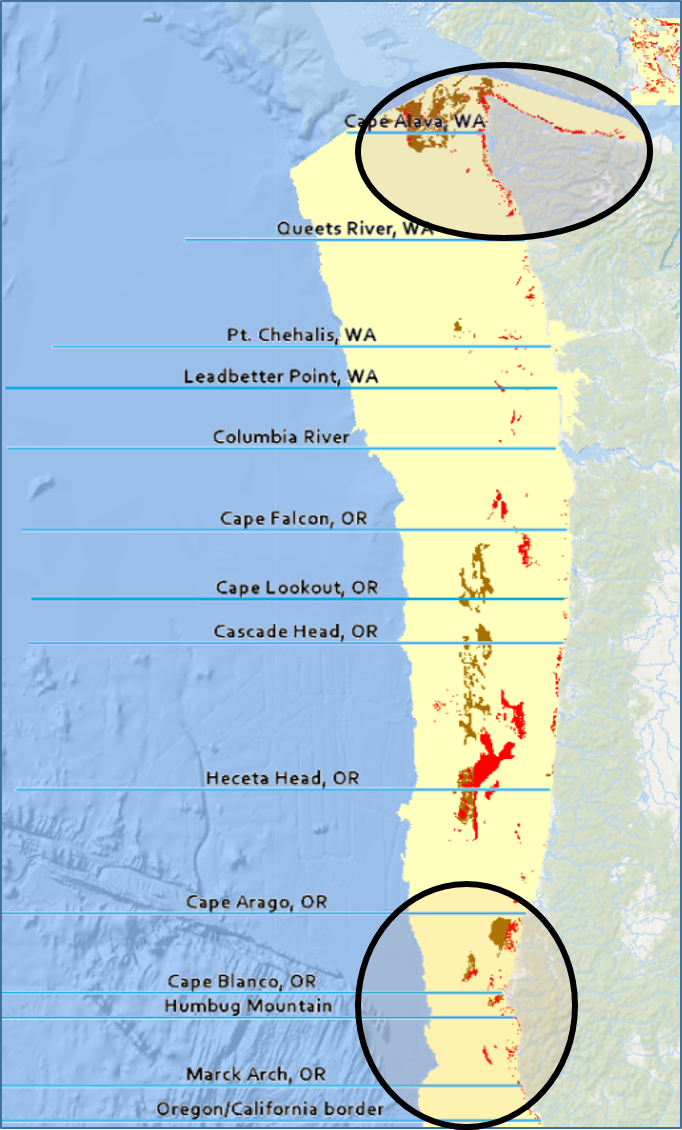
\includegraphics[width=1\textwidth,height=1\textheight]{C:/Users/Jason.Cope/Documents/Github/Vermilion rockfish OR WA assessment 2021/OR/write_up/figures/stock/Vermilion_Map.png}
\caption{Oregon and Washington coastlines with rocky habitat indicated by brown shaded areas. Circled areas represent areas of primary vermilion rockfish occurence..\label{fig:ORWA-map}}
\end{figure}

\tagmcend\tagstructend

\tagstructbegin{tag=Figure,alttext={Total mortality from the southern Oregon and northern Washington recreational fisheries. These represent ninty and ninty-seven percent of the total vermilion removals in each state, respectively..}}\tagmcbegin{tag=Figure}

\begin{figure}
\centering
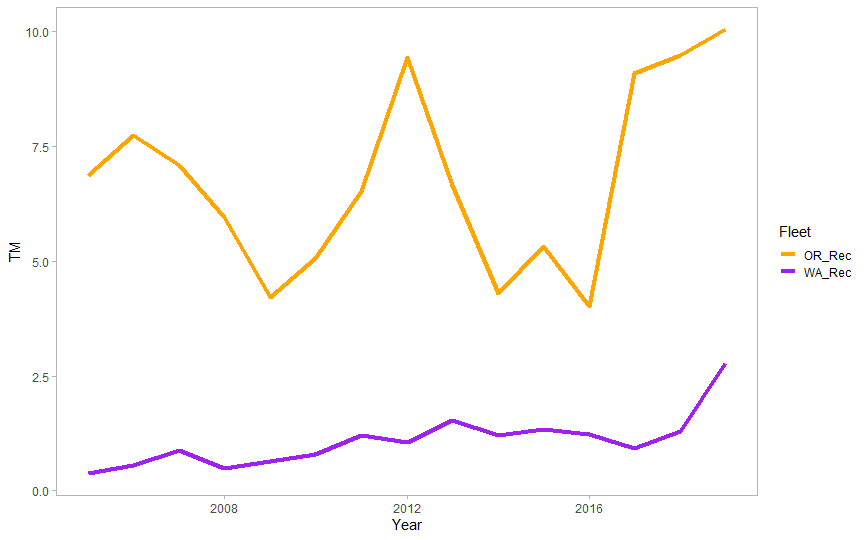
\includegraphics[width=1\textwidth,height=1\textheight]{C:/Users/Jason.Cope/Documents/Github/Vermilion rockfish OR WA assessment 2021/OR/write_up/figures/stock/TM_Vermilion_ORWA.png}
\caption{Total mortality from the southern Oregon and northern Washington recreational fisheries. These represent ninty and ninty-seven percent of the total vermilion removals in each state, respectively..\label{fig:tm-plot}}
\end{figure}

\tagmcend\tagstructend

\tagstructbegin{tag=Figure,alttext={Summary of data sources used in the base model.}}\tagmcbegin{tag=Figure}

\begin{figure}
\centering
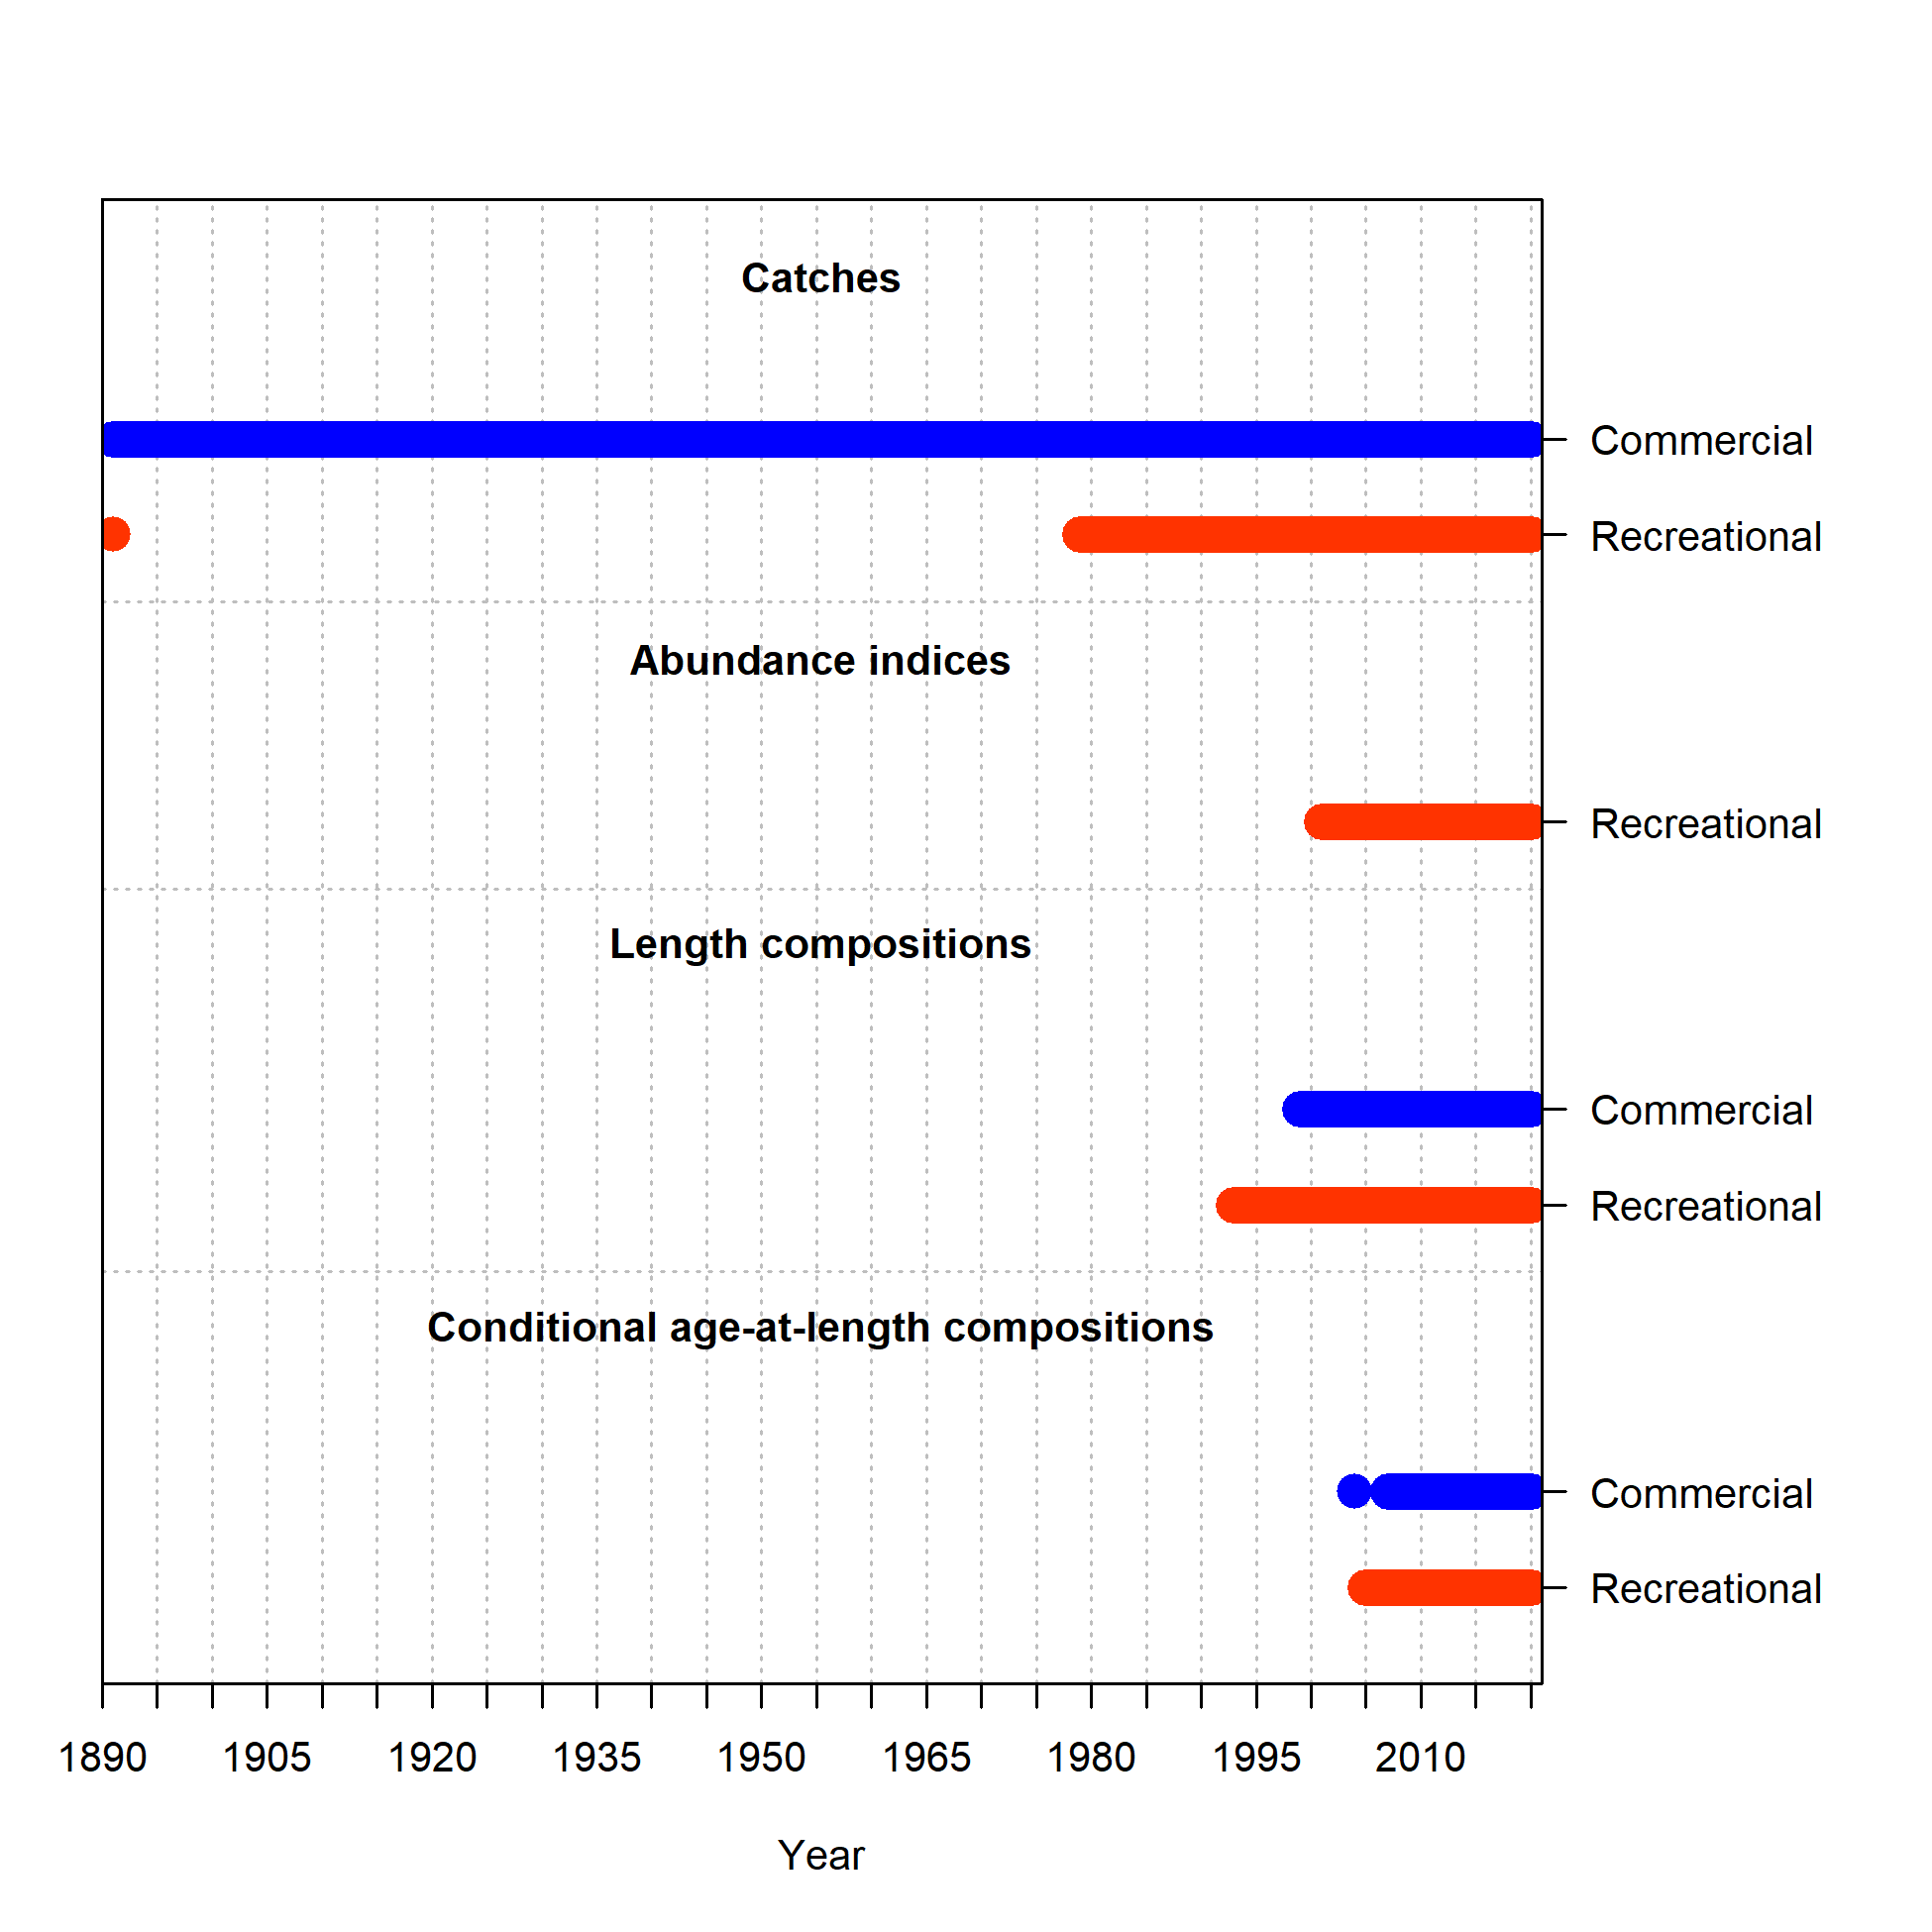
\includegraphics[width=1\textwidth,height=1\textheight]{C:/Users/Jason.Cope/Documents/Github/Vermilion rockfish OR WA assessment 2021/OR/write_up/models/Reference model/plots/data_plot.png}
\caption{Summary of data sources used in the base model.\label{fig:data-plot}}
\end{figure}

\tagmcend\tagstructend

\tagstructbegin{tag=Figure,alttext={Bubble plot of length compositions by year and fleet. Size of the bubble indicates higher proportion. All proportions within year sum to one.}}\tagmcbegin{tag=Figure}

\begin{figure}
\centering
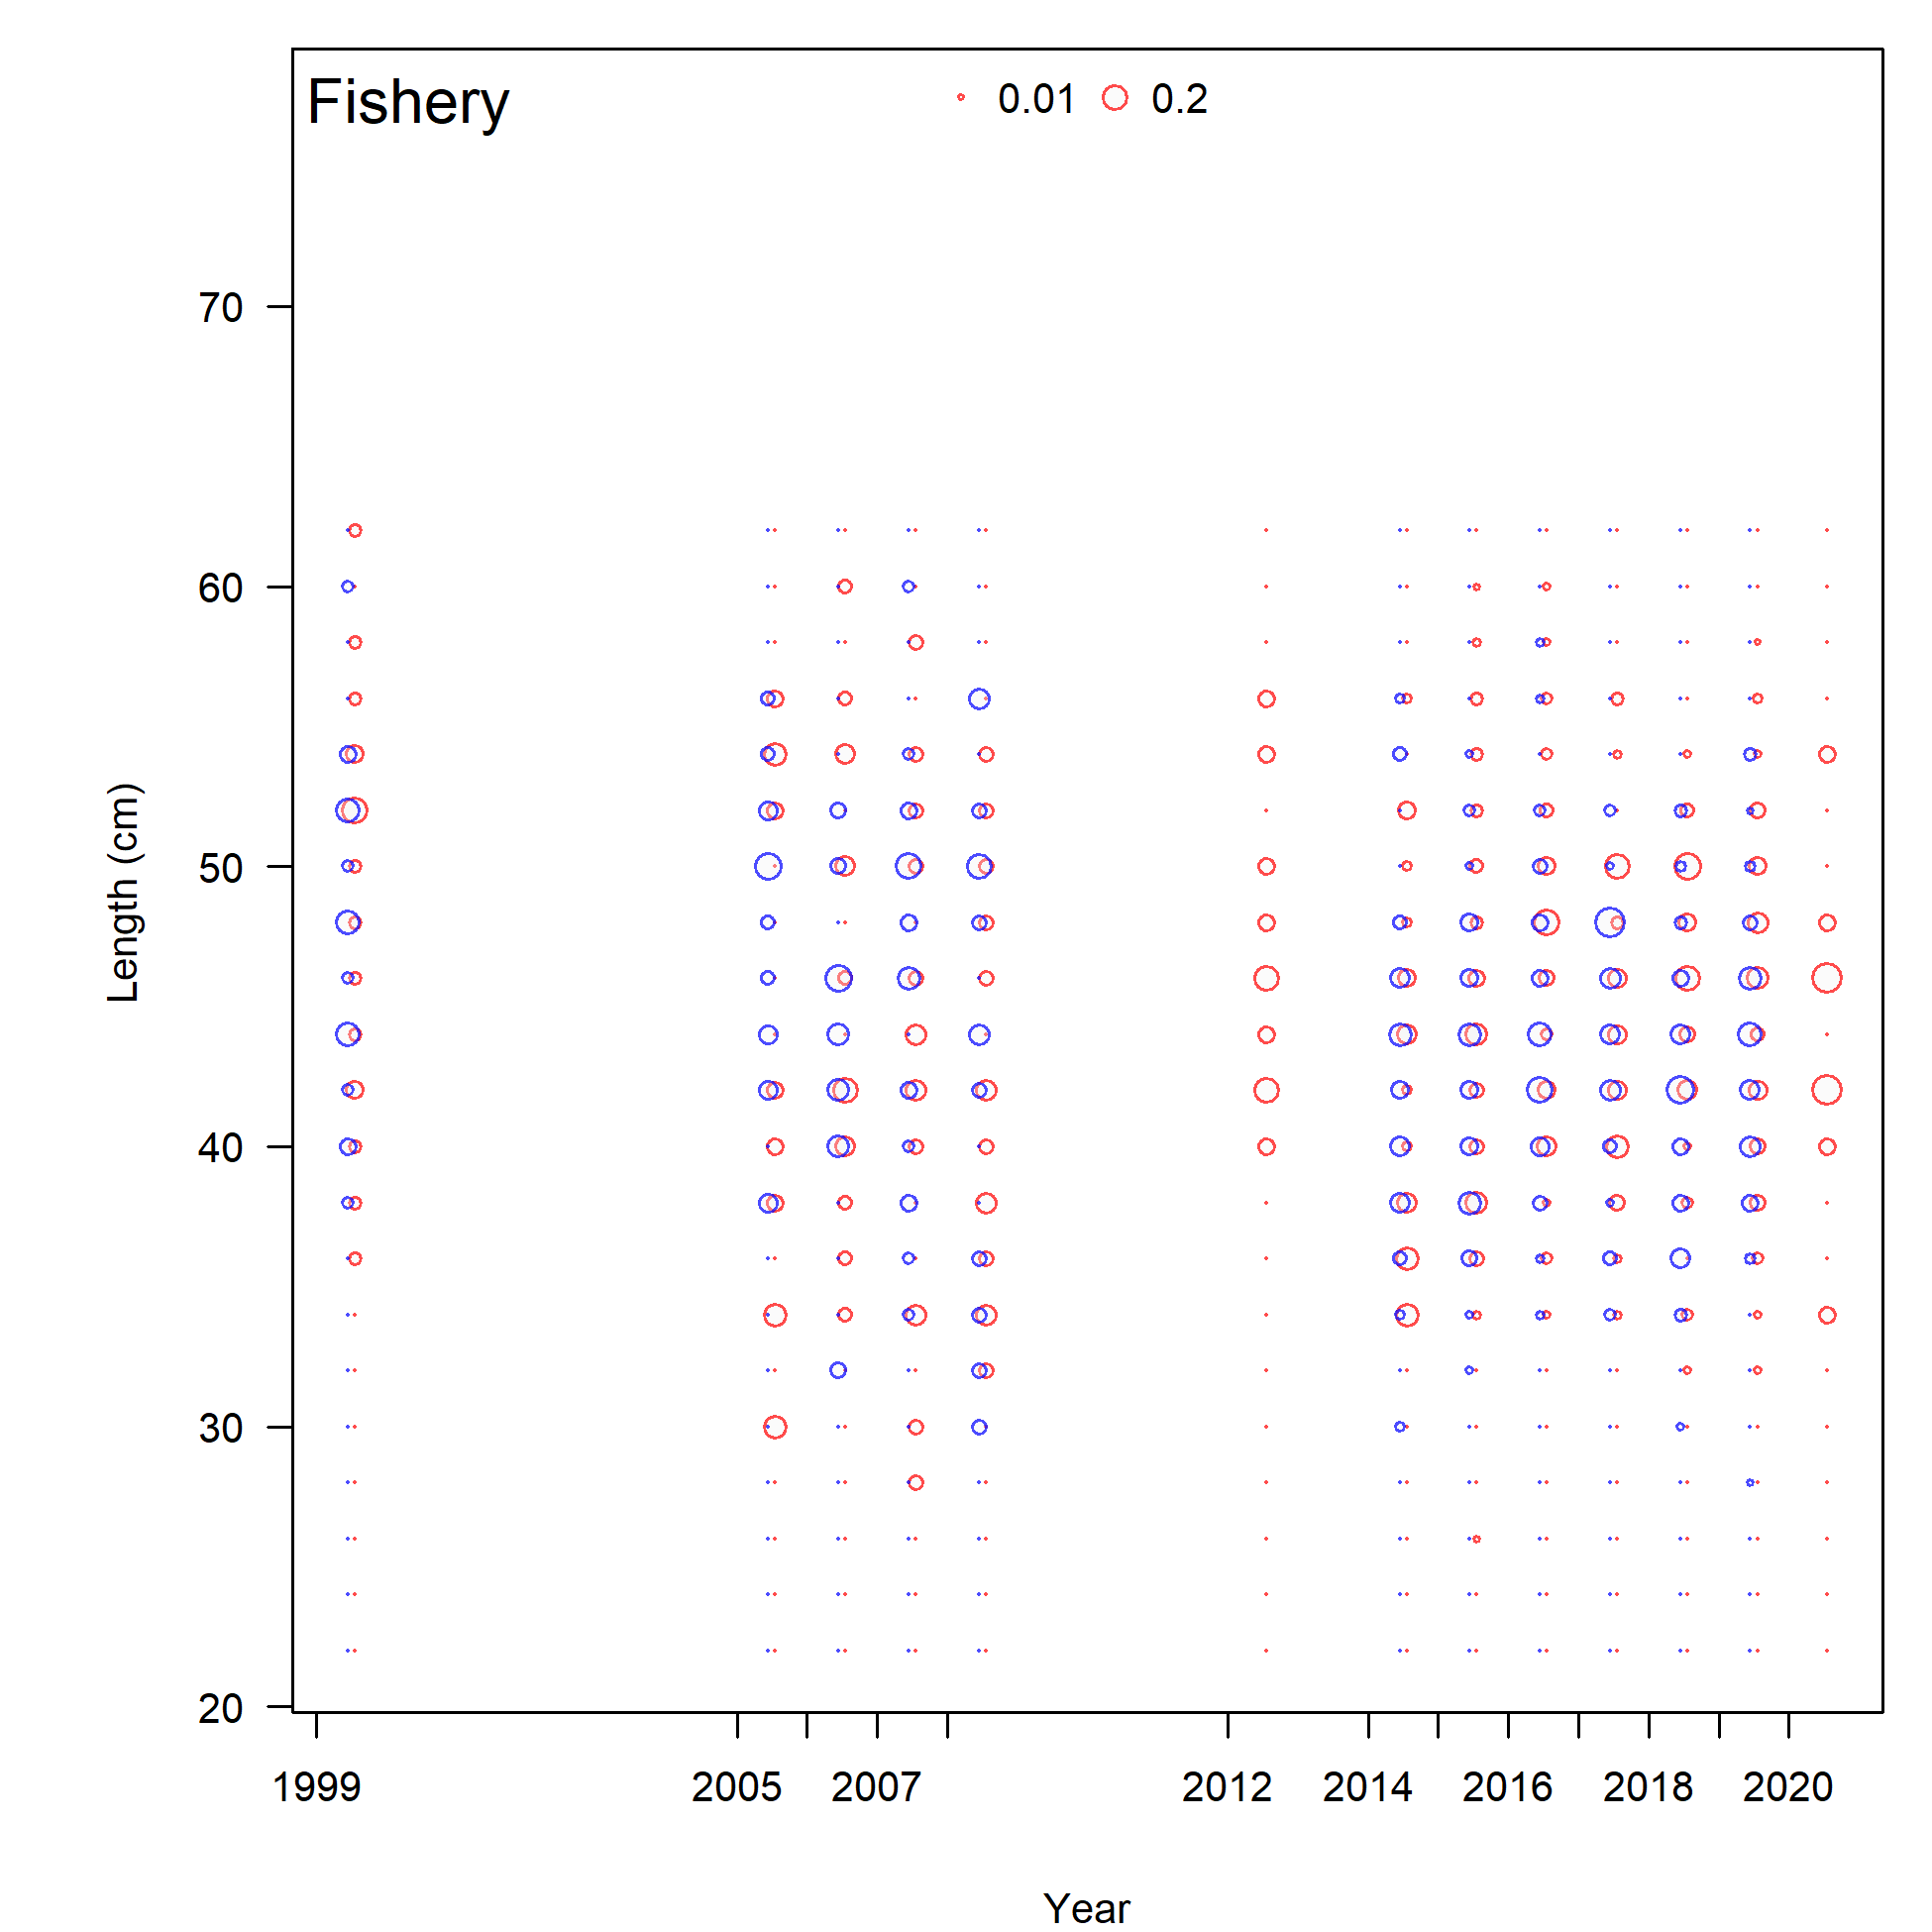
\includegraphics[width=1\textwidth,height=1\textheight]{C:/Users/Jason.Cope/Documents/Github/Vermilion rockfish OR WA assessment 2021/OR/write_up/models/Reference model/plots/comp_lendat__multi-fleet_comparison.png}
\caption{Bubble plot of length compositions by year and fleet. Size of the bubble indicates higher proportion. All proportions within year sum to one.\label{fig:comm-rec-lts_bubbs}}
\end{figure}

\tagmcend\tagstructend

\tagstructbegin{tag=Figure,alttext={Species coefficients (blue bars) for presence/absence of vermilion rockfish in the ORBS dockside index. Horizontal black bars represent the 95 percent confidence intervals.}}\tagmcbegin{tag=Figure}

\begin{figure}
\centering
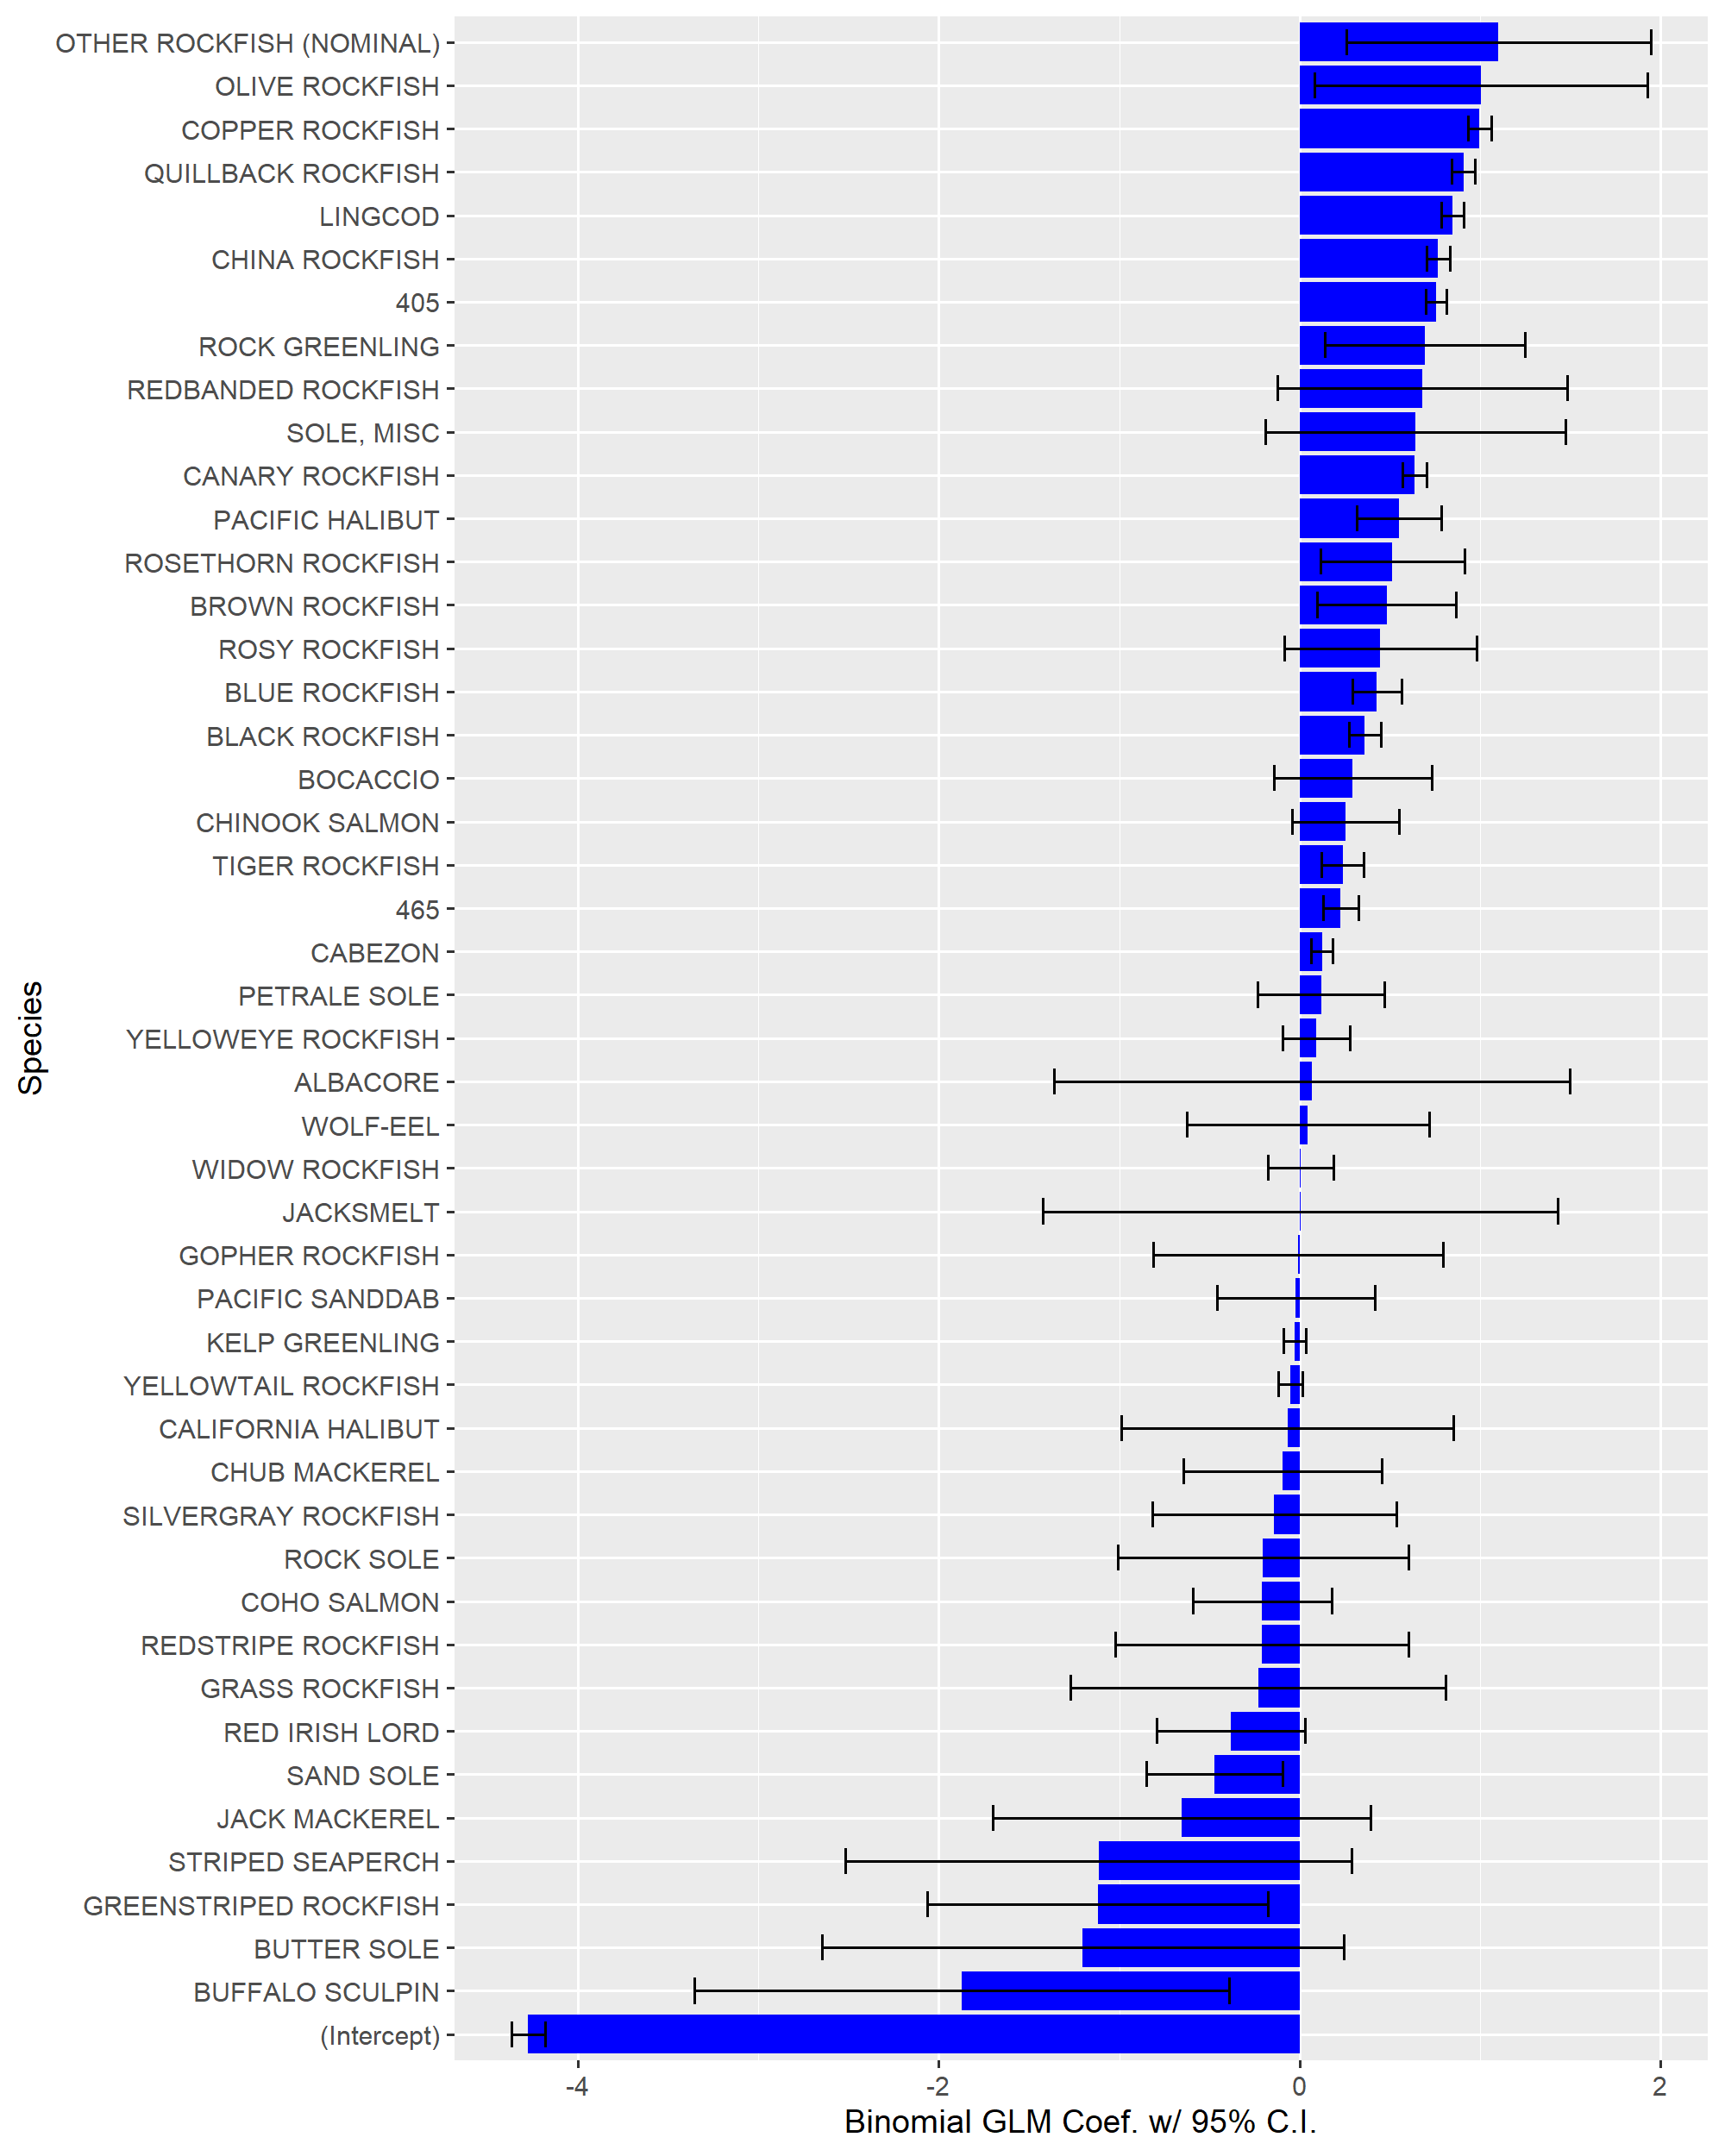
\includegraphics[width=1\textwidth,height=1\textheight]{C:/Users/Jason.Cope/Documents/Github/Vermilion rockfish OR WA assessment 2021/OR/write_up/figures/index/OR_ORBS_Index_S-M_coef.png}
\caption{Species coefficients (blue bars) for presence/absence of vermilion rockfish in the ORBS dockside index. Horizontal black bars represent the 95 percent confidence intervals.\label{fig:s-m-coef}}
\end{figure}

\tagmcend\tagstructend

\tagstructbegin{tag=Figure,alttext={The ORBS dockside area under the characteristic curve (AUC) plot, which represents the probability that a randomly chosen observation of presence would be assigned a higher ranked prediction than a randomly chosen observation of absence. Values much greater than 0.5 indicate a significant improvement over a random classifier (AUC = 0.5).}}\tagmcbegin{tag=Figure}

\begin{figure}
\centering
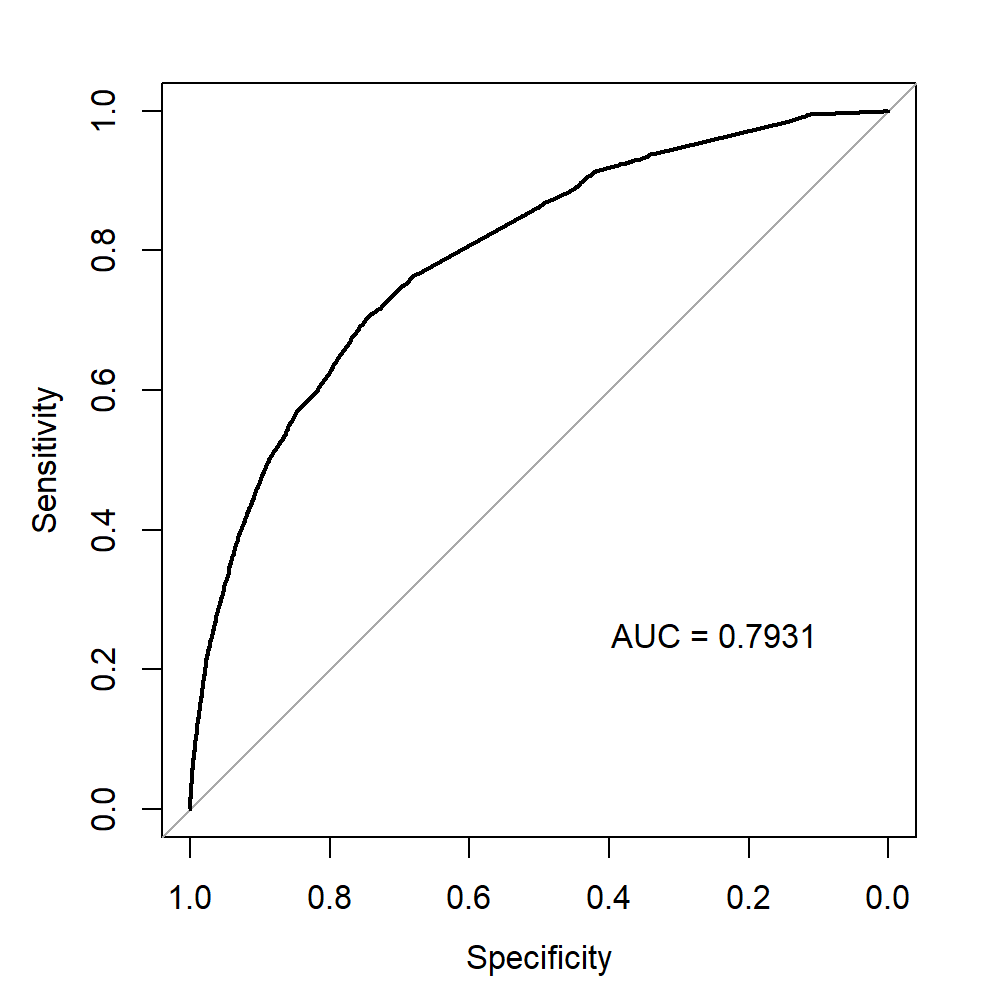
\includegraphics[width=1\textwidth,height=1\textheight]{C:/Users/Jason.Cope/Documents/Github/Vermilion rockfish OR WA assessment 2021/OR/write_up/figures/index/OR_ORBS_Index_S-M_ROC.png}
\caption{The ORBS dockside area under the characteristic curve (AUC) plot, which represents the probability that a randomly chosen observation of presence would be assigned a higher ranked prediction than a randomly chosen observation of absence. Values much greater than 0.5 indicate a significant improvement over a random classifier (AUC = 0.5).\label{fig:OR-ORBS-Index-S-M-ROC}}
\end{figure}

\tagmcend\tagstructend

\tagstructbegin{tag=Figure,alttext={Characterization of the final subset of ORBS dockside data used in the delta-GLM analyses to develop an index for vermilion rockfish.}}\tagmcbegin{tag=Figure}

\begin{figure}
\centering
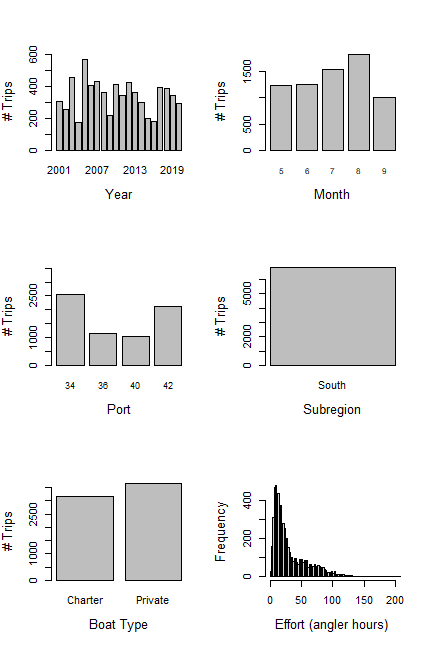
\includegraphics[width=1\textwidth,height=1\textheight]{C:/Users/Jason.Cope/Documents/Github/Vermilion rockfish OR WA assessment 2021/OR/write_up/figures/index/ORBS_DataSummary.png}
\caption{Characterization of the final subset of ORBS dockside data used in the delta-GLM analyses to develop an index for vermilion rockfish.\label{fig:ORBS-DataSummary}}
\end{figure}

\tagmcend\tagstructend

\tagstructbegin{tag=Figure,alttext={The distribution of trip-level raw positive catch CPUE for the ORBS dockside data relative to potential covariates evaluated in the vermilion rockfish delta-GLM analysis.}}\tagmcbegin{tag=Figure}

\begin{figure}
\centering
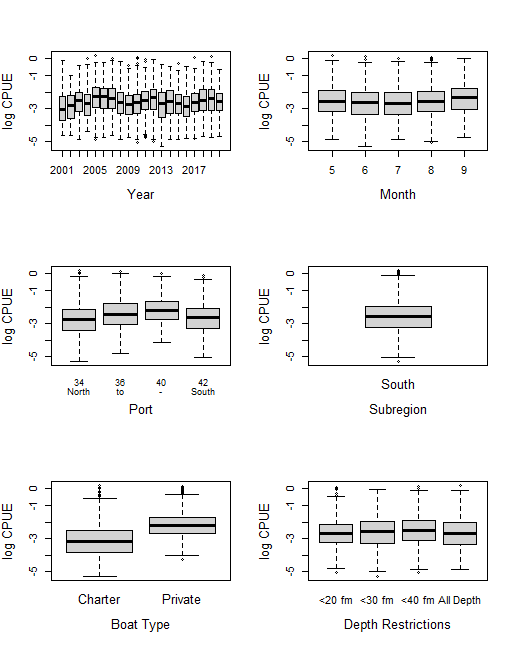
\includegraphics[width=1\textwidth,height=1\textheight]{C:/Users/Jason.Cope/Documents/Github/Vermilion rockfish OR WA assessment 2021/OR/write_up/figures/index/ORBS_CPUESummary.png}
\caption{The distribution of trip-level raw positive catch CPUE for the ORBS dockside data relative to potential covariates evaluated in the vermilion rockfish delta-GLM analysis.\label{fig:ORBS-CPUESummary}}
\end{figure}

\tagmcend\tagstructend

\tagstructbegin{tag=Figure,alttext={Scaled quantile-quantile plot (left) and rank-transformed versus standardized residuals (right) for the binomial model of the ORBS dockside index.}}\tagmcbegin{tag=Figure}

\begin{figure}
\centering
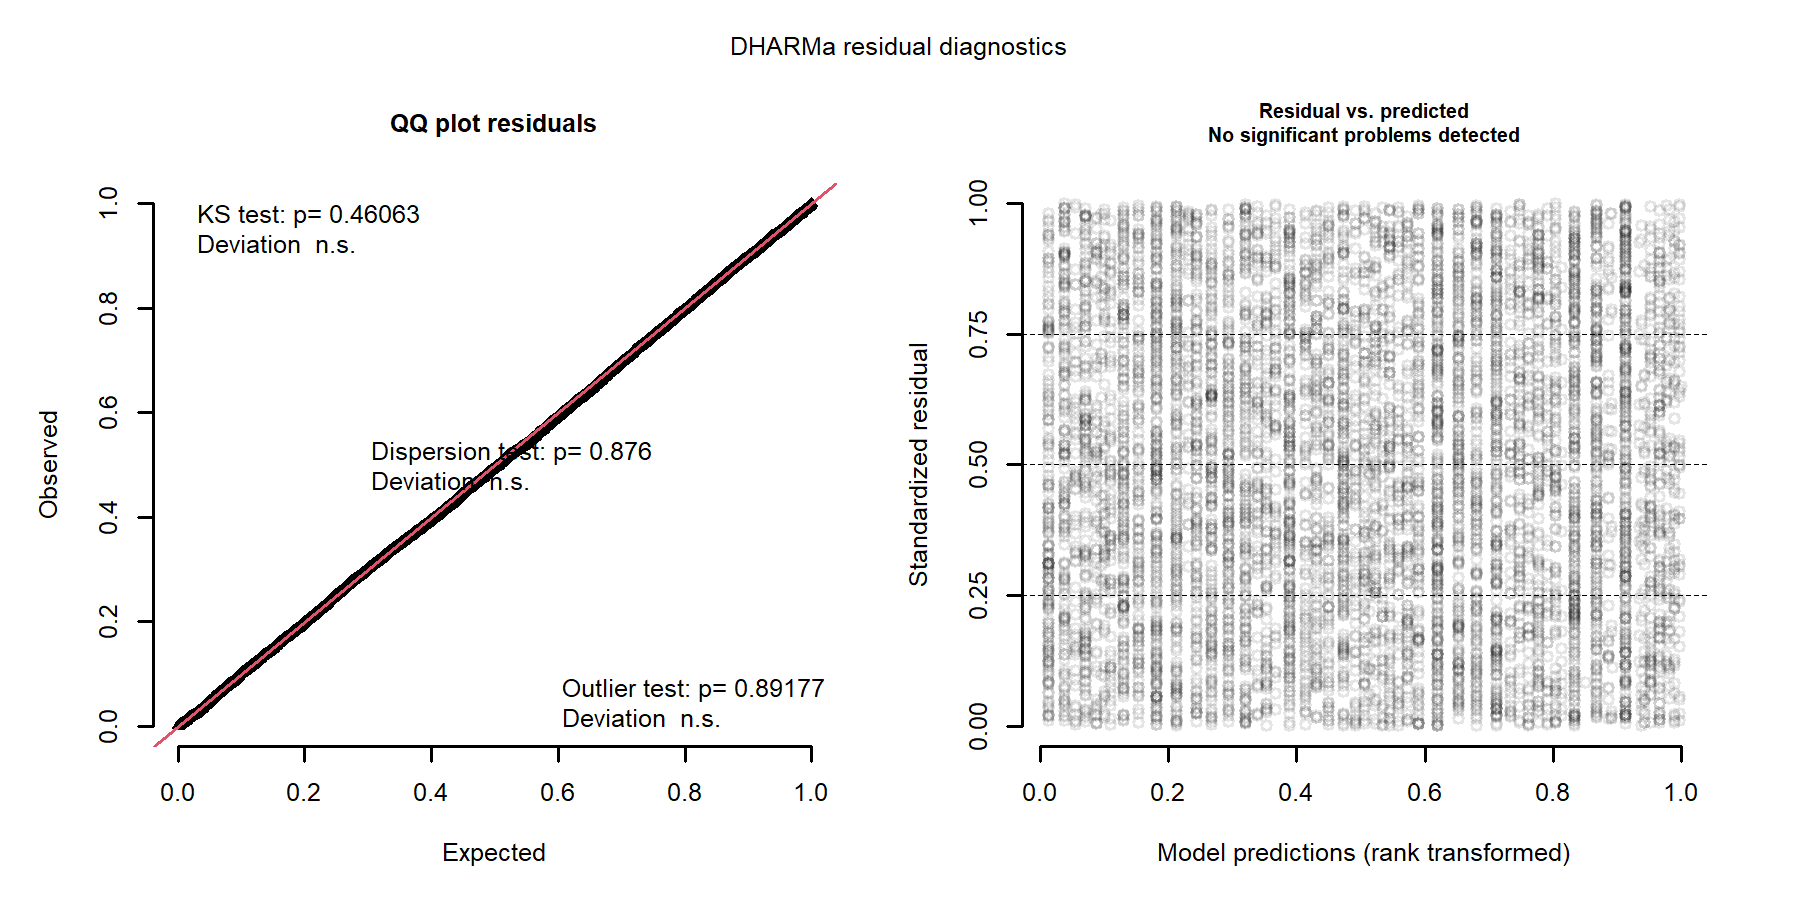
\includegraphics[width=1\textwidth,height=1\textheight]{C:/Users/Jason.Cope/Documents/Github/Vermilion rockfish OR WA assessment 2021/OR/write_up/figures/index/ScaledQQplot_bin.png}
\caption{Scaled quantile-quantile plot (left) and rank-transformed versus standardized residuals (right) for the binomial model of the ORBS dockside index.\label{fig:ScaledQQplot-bin}}
\end{figure}

\tagmcend\tagstructend

\tagstructbegin{tag=Figure,alttext={Scaled quantile-quantile plot (left) and rank-transformed versus standardized residuals (right) for the positive model of the ORBS dockside index.}}\tagmcbegin{tag=Figure}

\begin{figure}
\centering
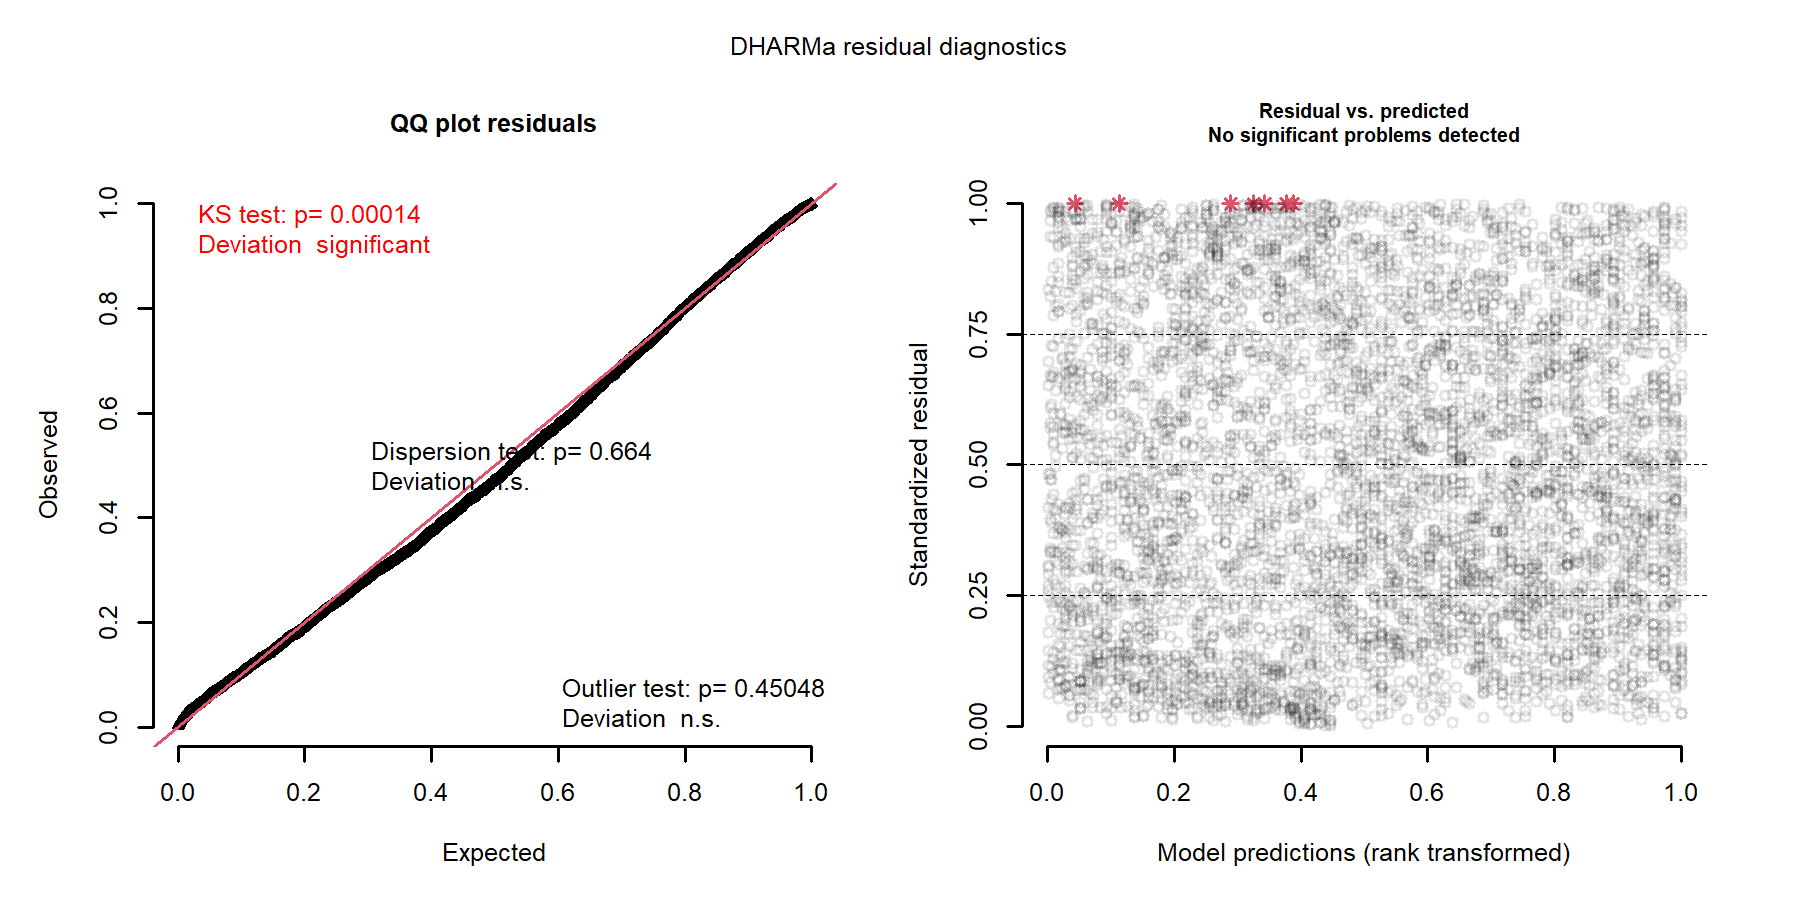
\includegraphics[width=1\textwidth,height=1\textheight]{C:/Users/Jason.Cope/Documents/Github/Vermilion rockfish OR WA assessment 2021/OR/write_up/figures/index/ScaledQQplot_pos.png}
\caption{Scaled quantile-quantile plot (left) and rank-transformed versus standardized residuals (right) for the positive model of the ORBS dockside index.\label{fig:ScaledQQplot-pos}}
\end{figure}

\tagmcend\tagstructend

\tagstructbegin{tag=Figure,alttext={Final ORBS dockside index for vermilion rockfish.}}\tagmcbegin{tag=Figure}

\begin{figure}
\centering
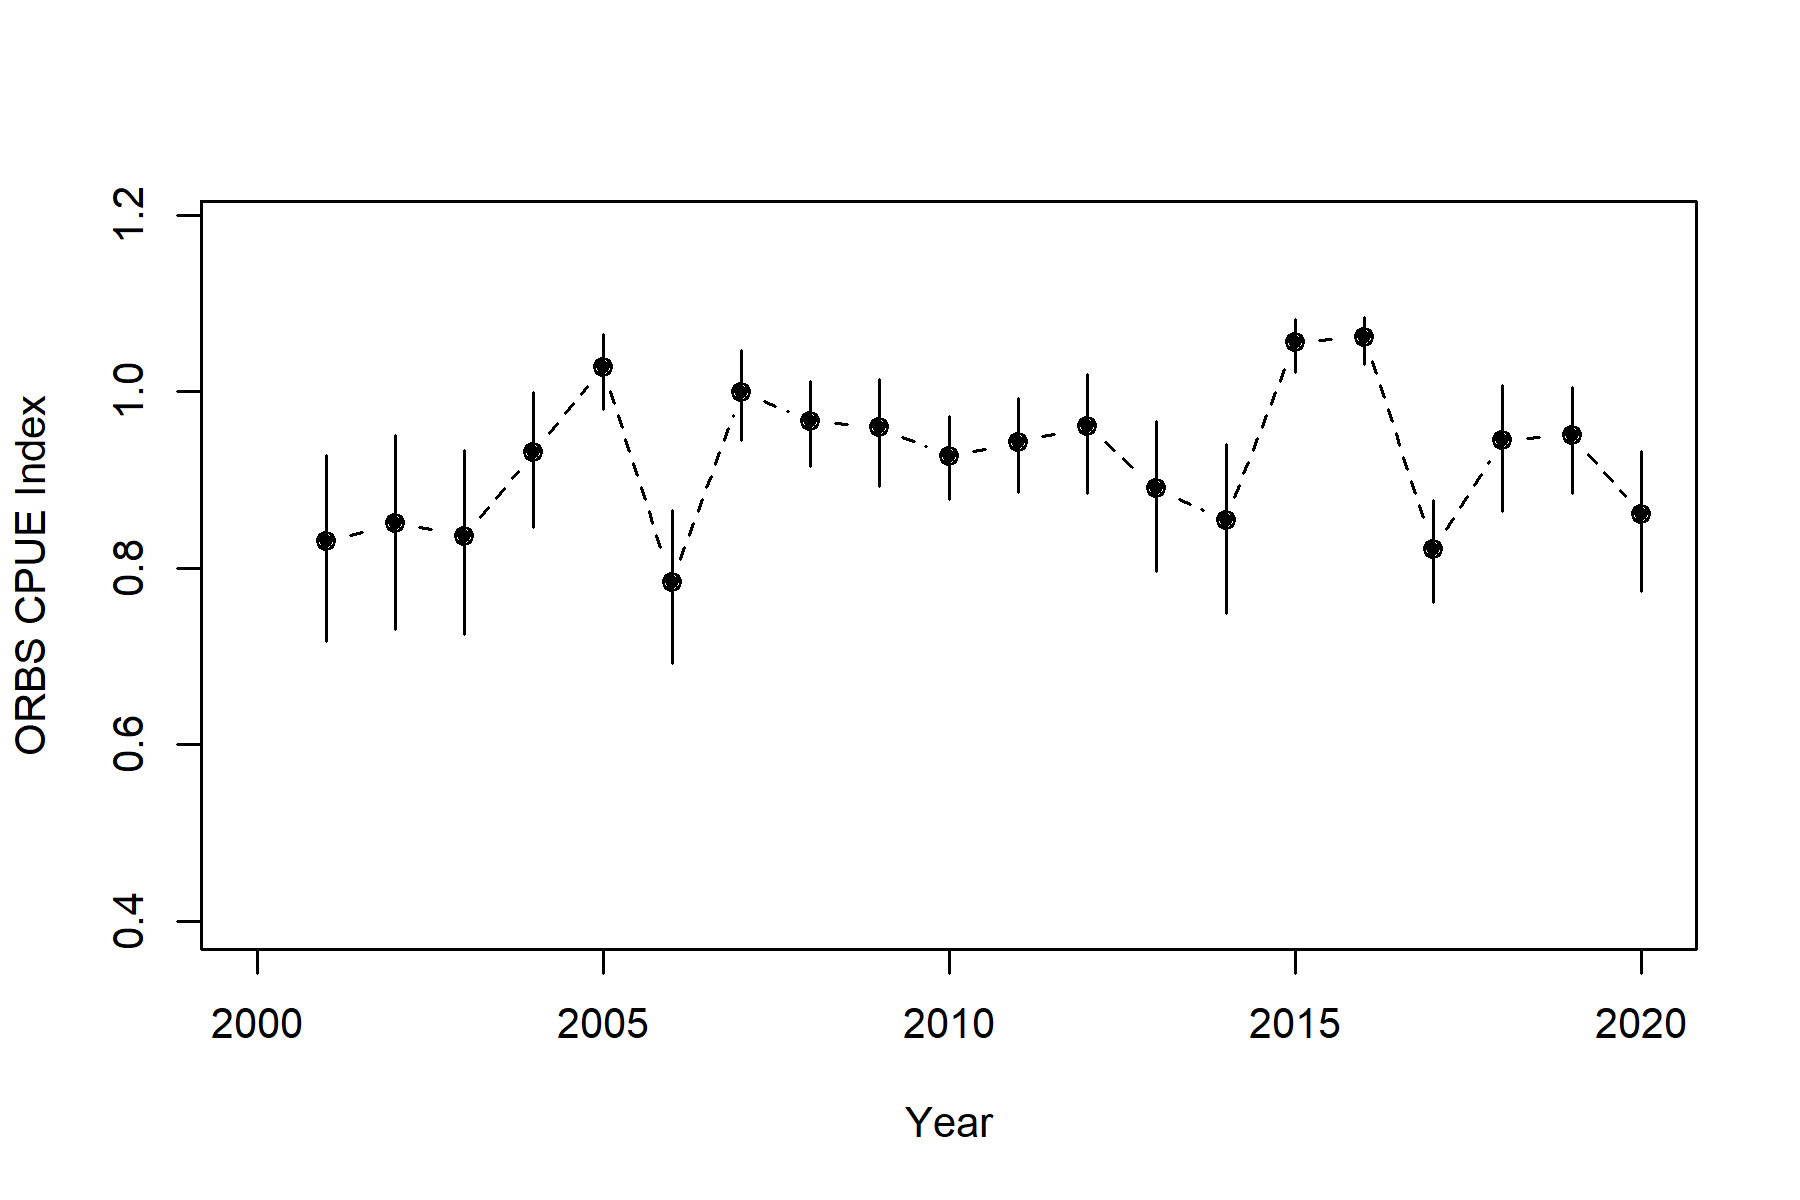
\includegraphics[width=1\textwidth,height=1\textheight]{C:/Users/Jason.Cope/Documents/Github/Vermilion rockfish OR WA assessment 2021/OR/write_up/figures/index/ORBS_OR_Dockside_Index.png}
\caption{Final ORBS dockside index for vermilion rockfish.\label{fig:ORBS-OR-Dockside-Index}}
\end{figure}

\tagmcend\tagstructend

\tagstructbegin{tag=Figure,alttext={Comparison of data distribution for vermilion rockfish CPUE to model-generated replicate data sets used to evaluate uncertainty for the binomial model component.}}\tagmcbegin{tag=Figure}

\begin{figure}
\centering
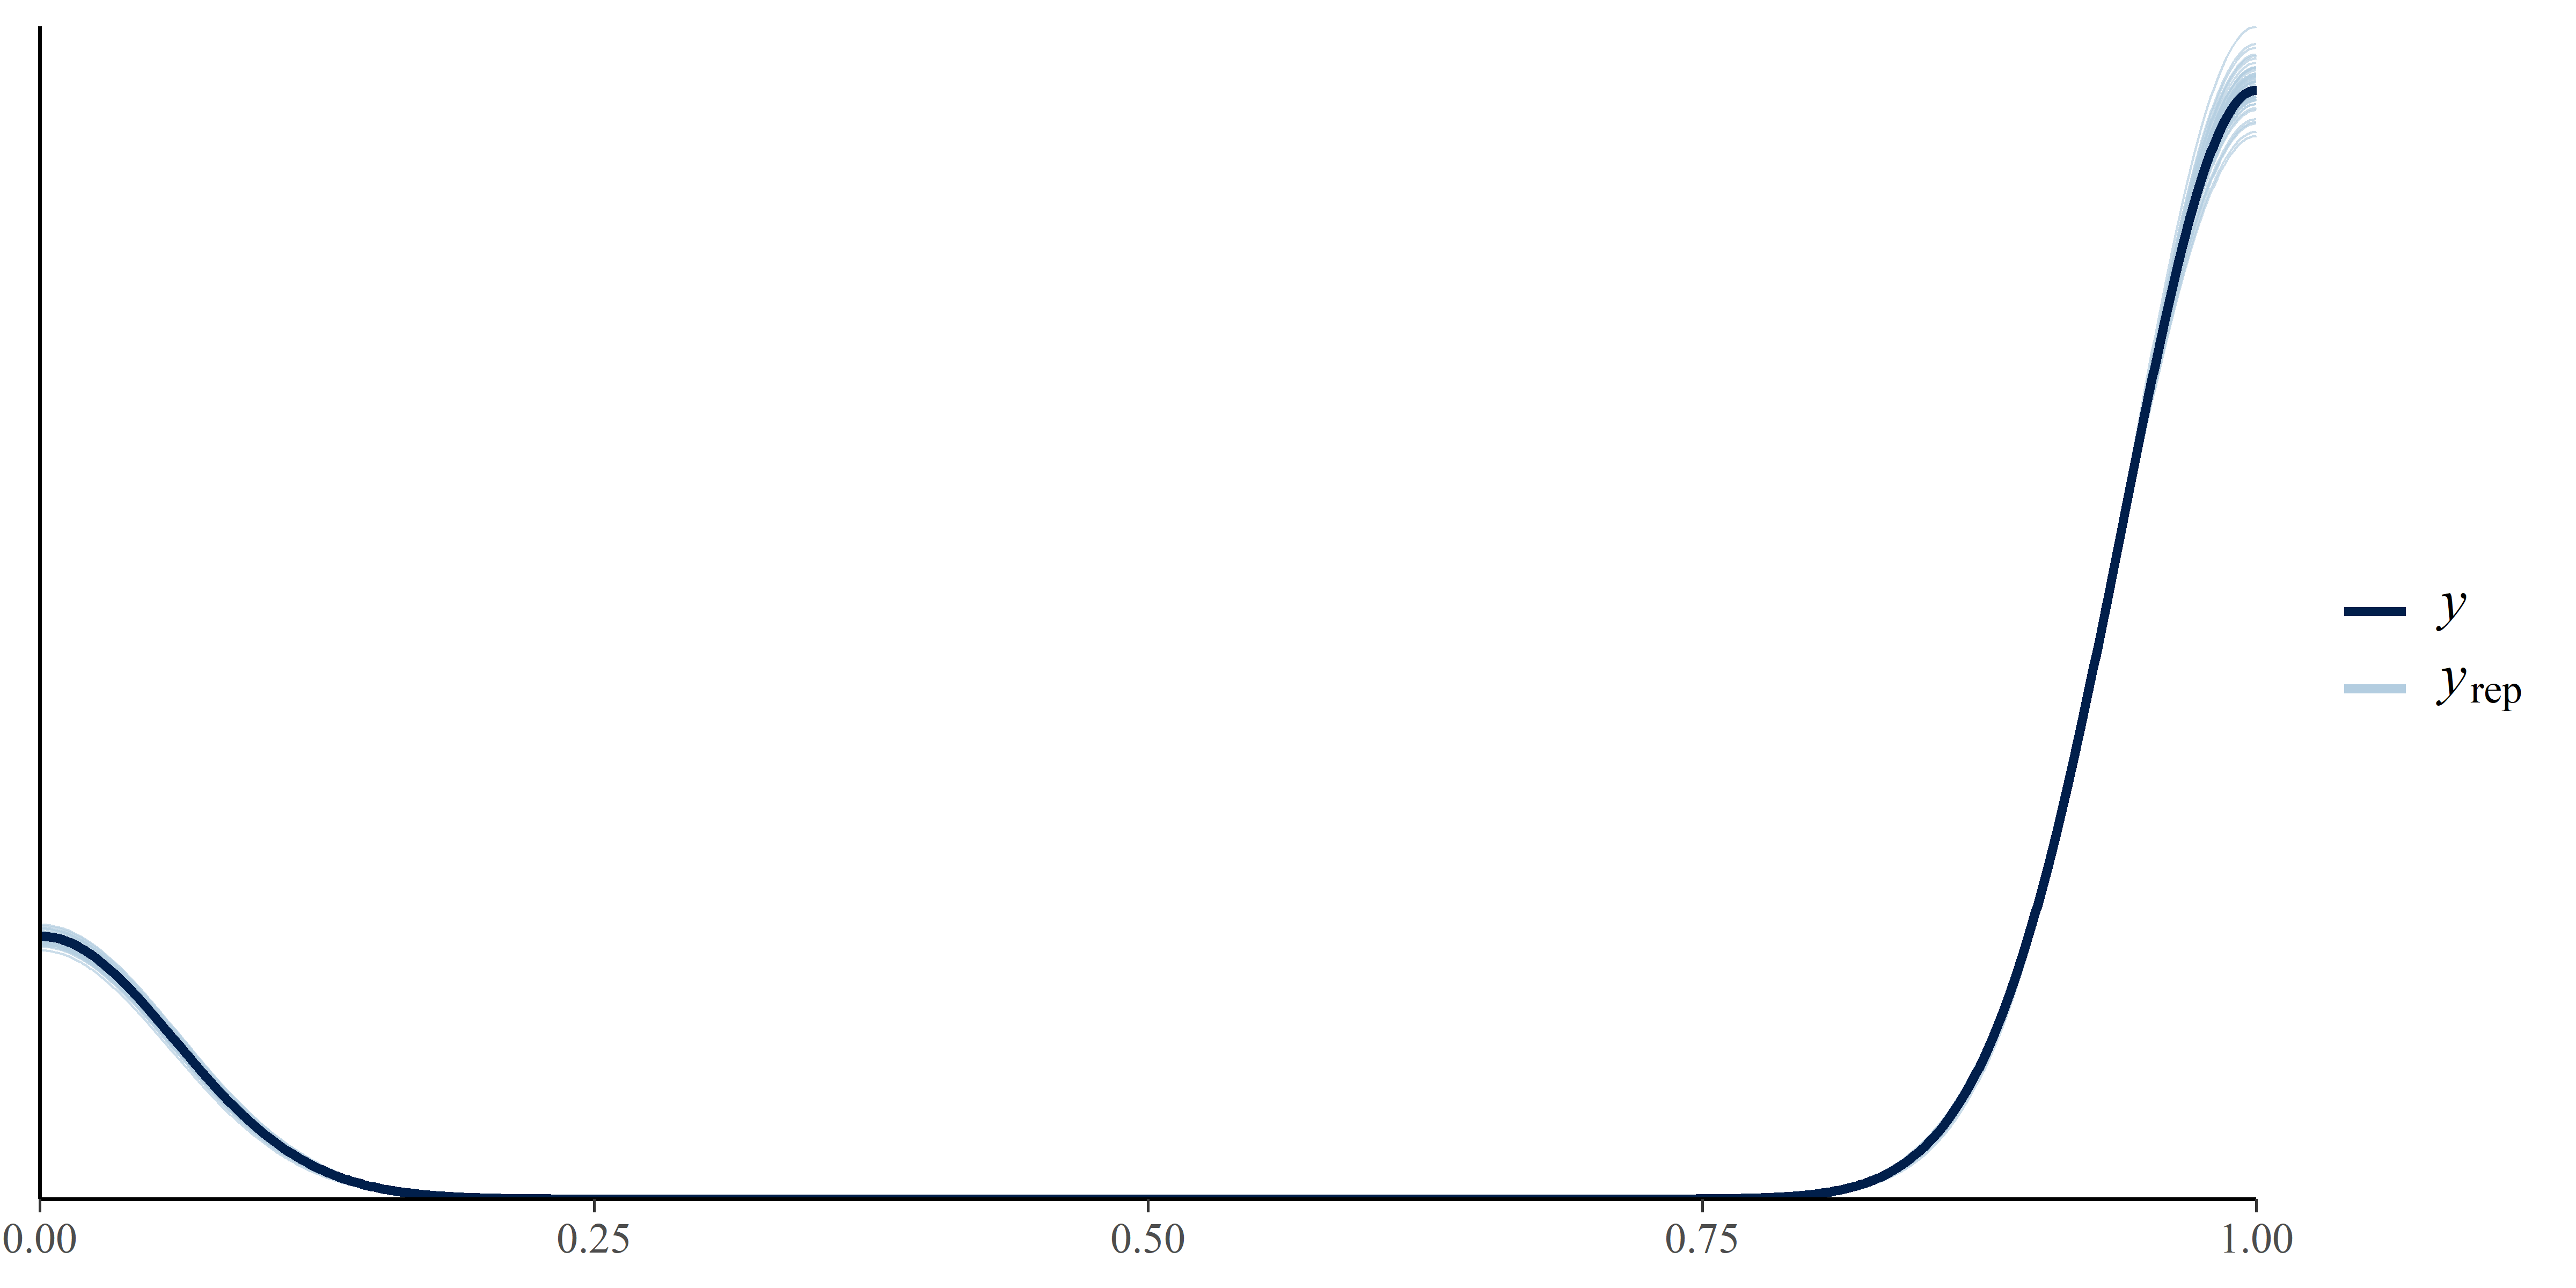
\includegraphics[width=1\textwidth,height=1\textheight]{C:/Users/Jason.Cope/Documents/Github/Vermilion rockfish OR WA assessment 2021/OR/write_up/figures/index/prop_zeros_bin_interaction.png}
\caption{Comparison of data distribution for vermilion rockfish CPUE to model-generated replicate data sets used to evaluate uncertainty for the binomial model component.\label{fig:prop-zeros-bin-interaction}}
\end{figure}

\tagmcend\tagstructend

\tagstructbegin{tag=Figure,alttext={Comparison of data distribution for vermilion rockfish CPUE to model-generated replicate data sets used to evaluate uncertainty for the positive model component.}}\tagmcbegin{tag=Figure}

\begin{figure}
\centering
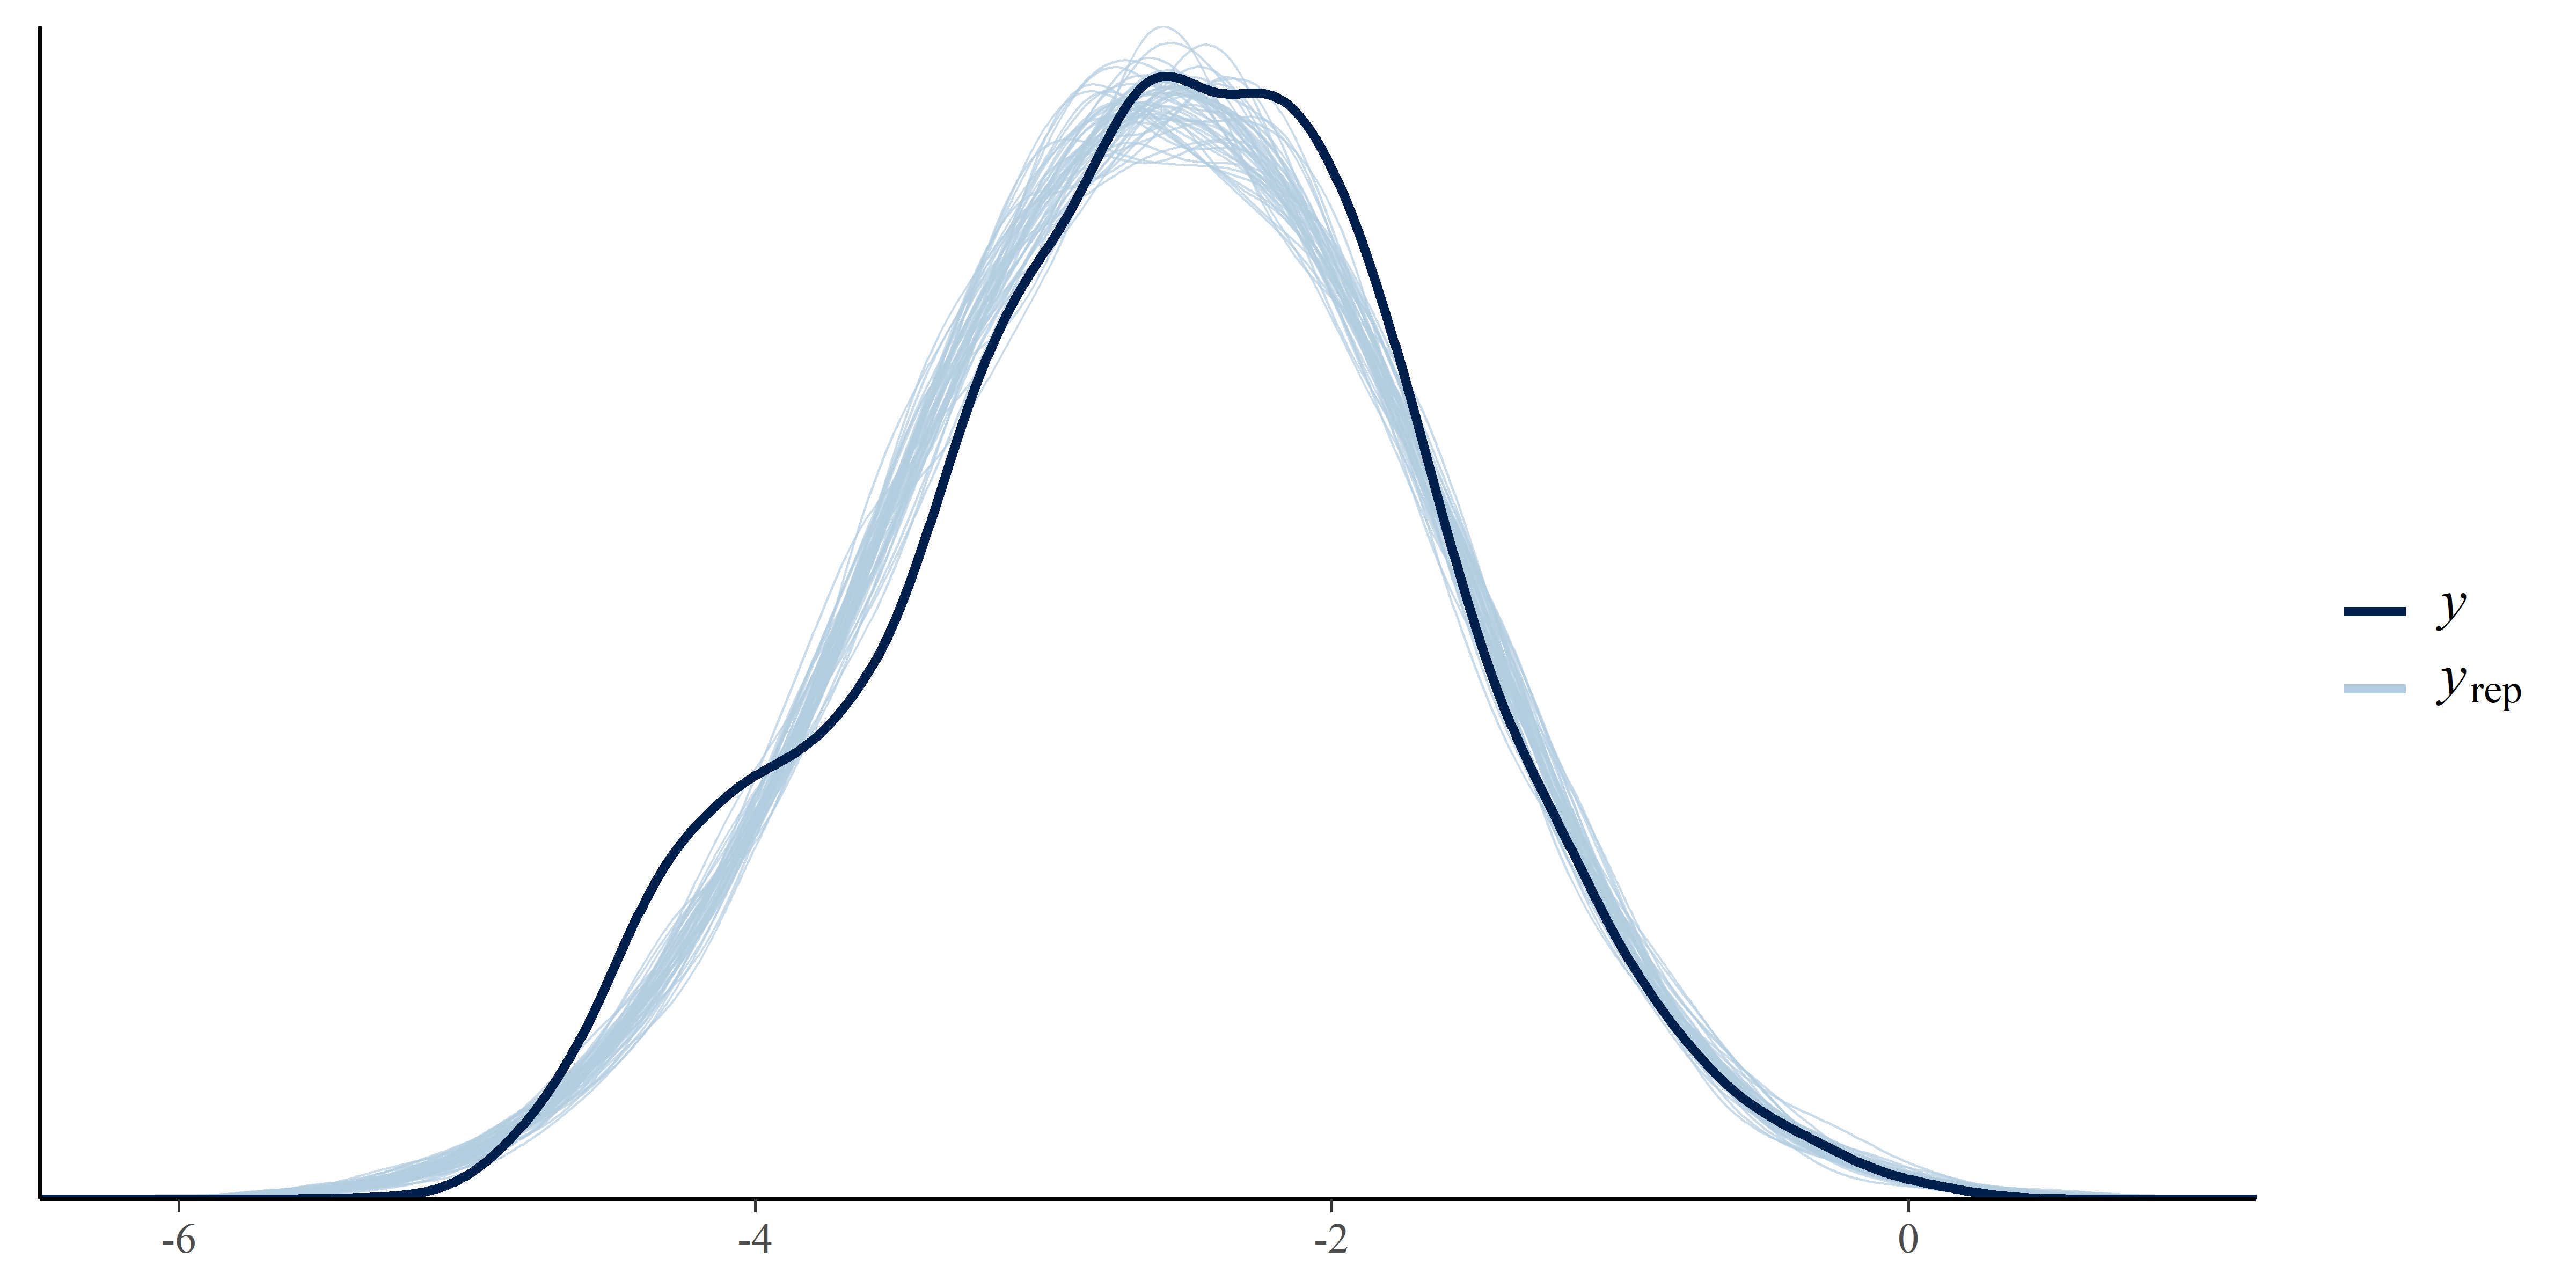
\includegraphics[width=1\textwidth,height=1\textheight]{C:/Users/Jason.Cope/Documents/Github/Vermilion rockfish OR WA assessment 2021/OR/write_up/figures/index/prop_zeros_pos.png}
\caption{Comparison of data distribution for vermilion rockfish CPUE to model-generated replicate data sets used to evaluate uncertainty for the positive model component.\label{fig:prop-zeros-pos}}
\end{figure}

\tagmcend\tagstructend

\tagstructbegin{tag=Figure,alttext={Observed length-at-age by data source and sex. Lines indicate fits to the von Bertalanffy growth equation, with parameter estimates provided in the bottom right corner of the figure.}}\tagmcbegin{tag=Figure}

\begin{figure}
\centering
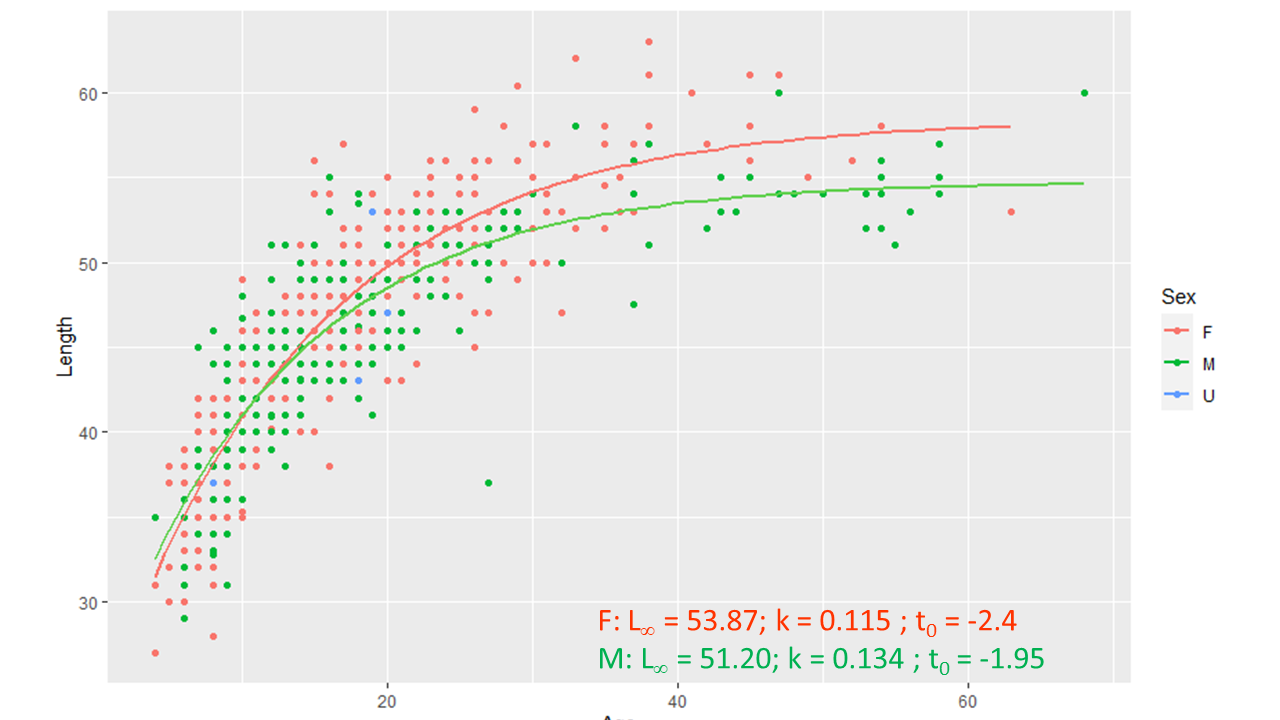
\includegraphics[width=1\textwidth,height=1\textheight]{C:/Users/Jason.Cope/Documents/Github/Vermilion rockfish OR WA assessment 2021/OR/write_up/figures/biology_plots/AG_plot_lines_parameters.png}
\caption{Observed length-at-age by data source and sex. Lines indicate fits to the von Bertalanffy growth equation, with parameter estimates provided in the bottom right corner of the figure.\label{fig:len-age-data}}
\end{figure}

\tagmcend\tagstructend

\tagstructbegin{tag=Figure,alttext={Model estimated length-at-age in the beginning of the year. Shaded area indicates 95 percent distribution of length-at-age around the estimated growth curve.}}\tagmcbegin{tag=Figure}

\begin{figure}
\centering
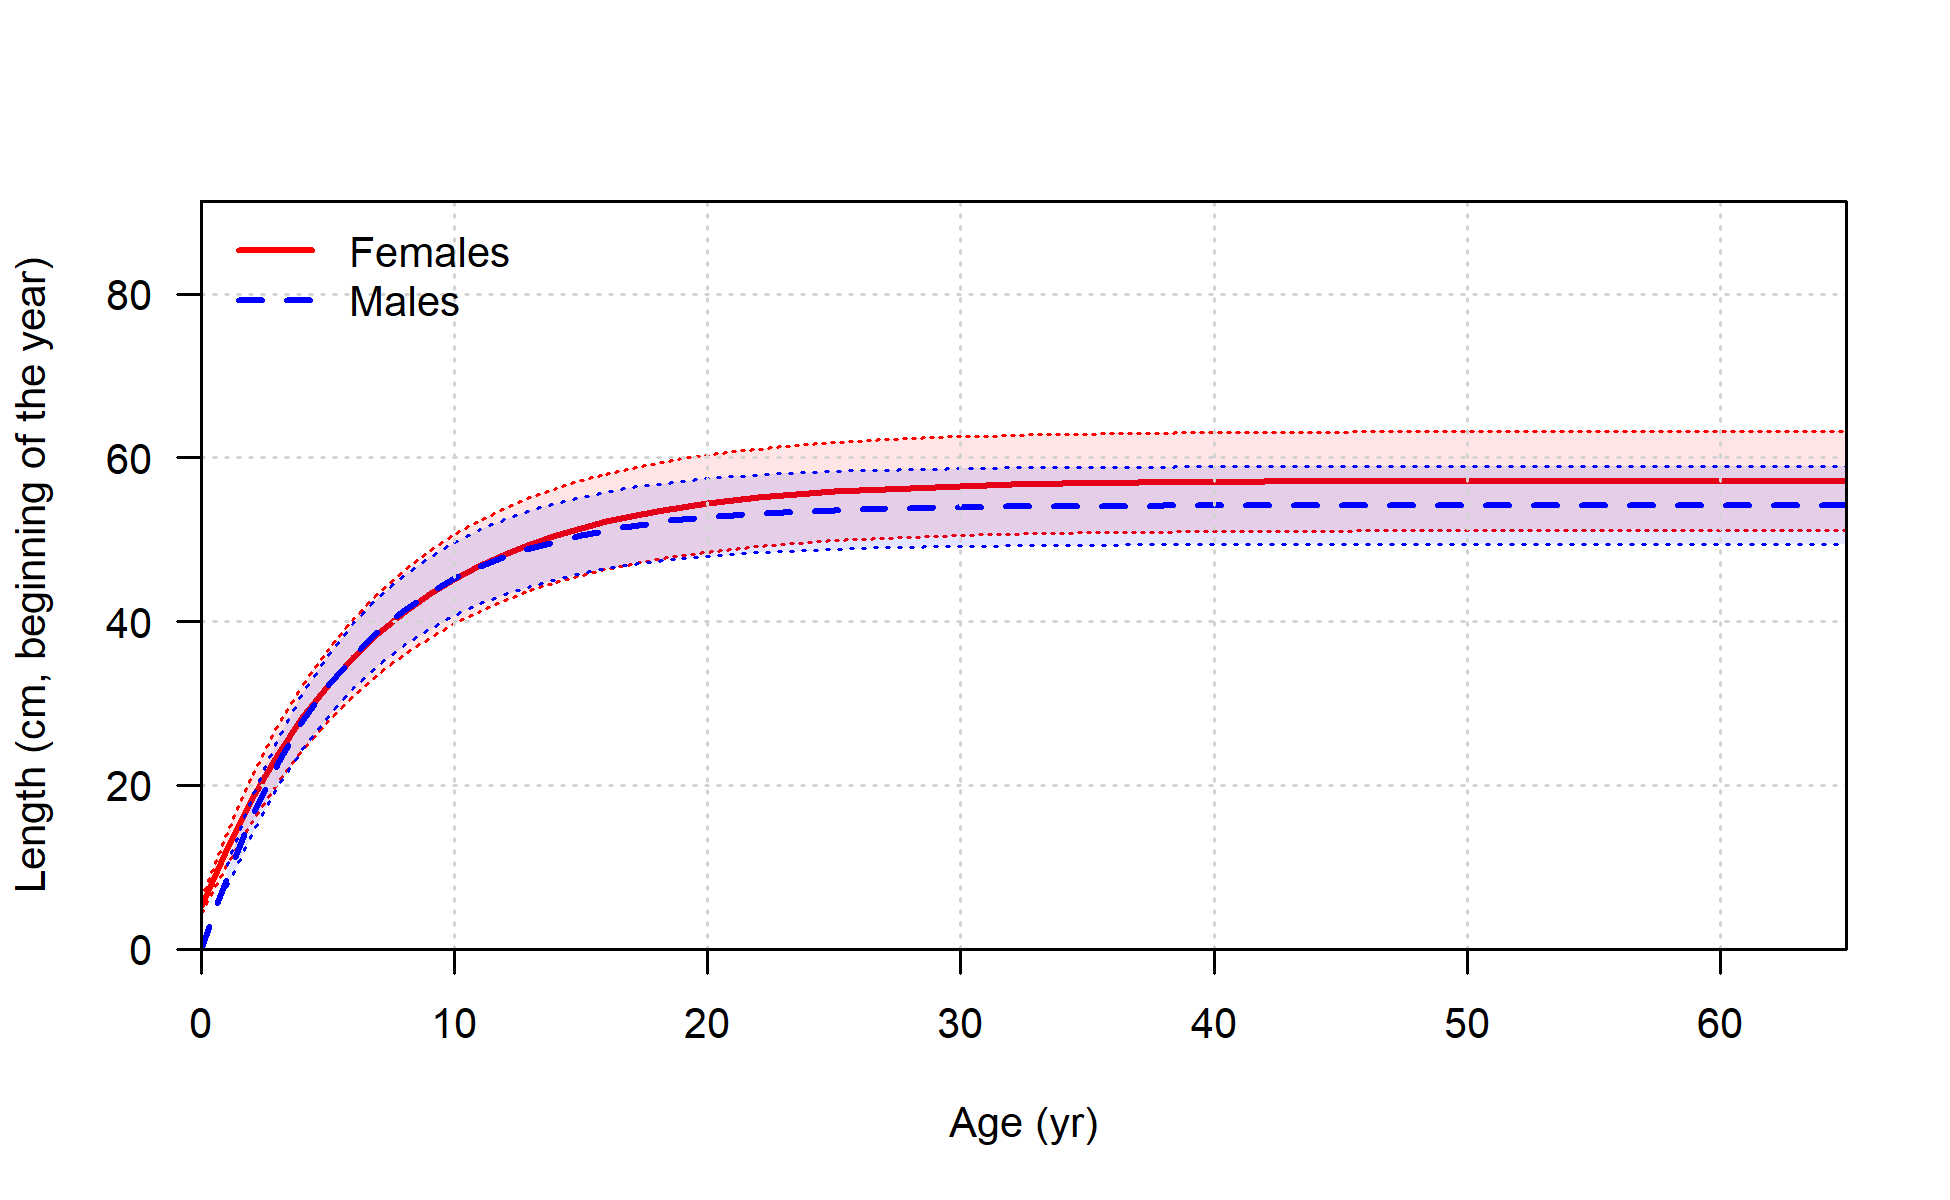
\includegraphics[width=1\textwidth,height=1\textheight]{C:/Users/Jason.Cope/Documents/Github/Vermilion rockfish OR WA assessment 2021/OR/write_up/models/Reference model/plots/bio1_sizeatage.png}
\caption{Model estimated length-at-age in the beginning of the year. Shaded area indicates 95 percent distribution of length-at-age around the estimated growth curve.\label{fig:len-age-ss}}
\end{figure}

\tagmcend\tagstructend

\tagstructbegin{tag=Figure,alttext={Agein error matrix (age by standard deviation) values by source. The commercial and recreational matrices are based on inter-reader comparisons.}}\tagmcbegin{tag=Figure}

\begin{figure}
\centering
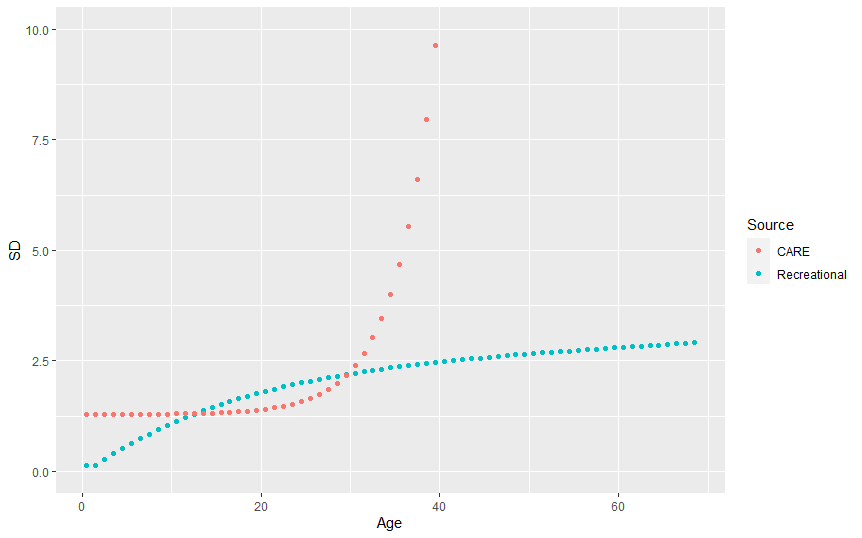
\includegraphics[width=1\textwidth,height=1\textheight]{C:/Users/Jason.Cope/Documents/Github/Vermilion rockfish OR WA assessment 2021/OR/write_up/figures/biology_plots/Age_error_plot.png}
\caption{Agein error matrix (age by standard deviation) values by source. The commercial and recreational matrices are based on inter-reader comparisons.\label{fig:age-error}}
\end{figure}

\tagmcend\tagstructend

\tagstructbegin{tag=Figure,alttext={Maturity as a function of  length.}}\tagmcbegin{tag=Figure}

\begin{figure}
\centering
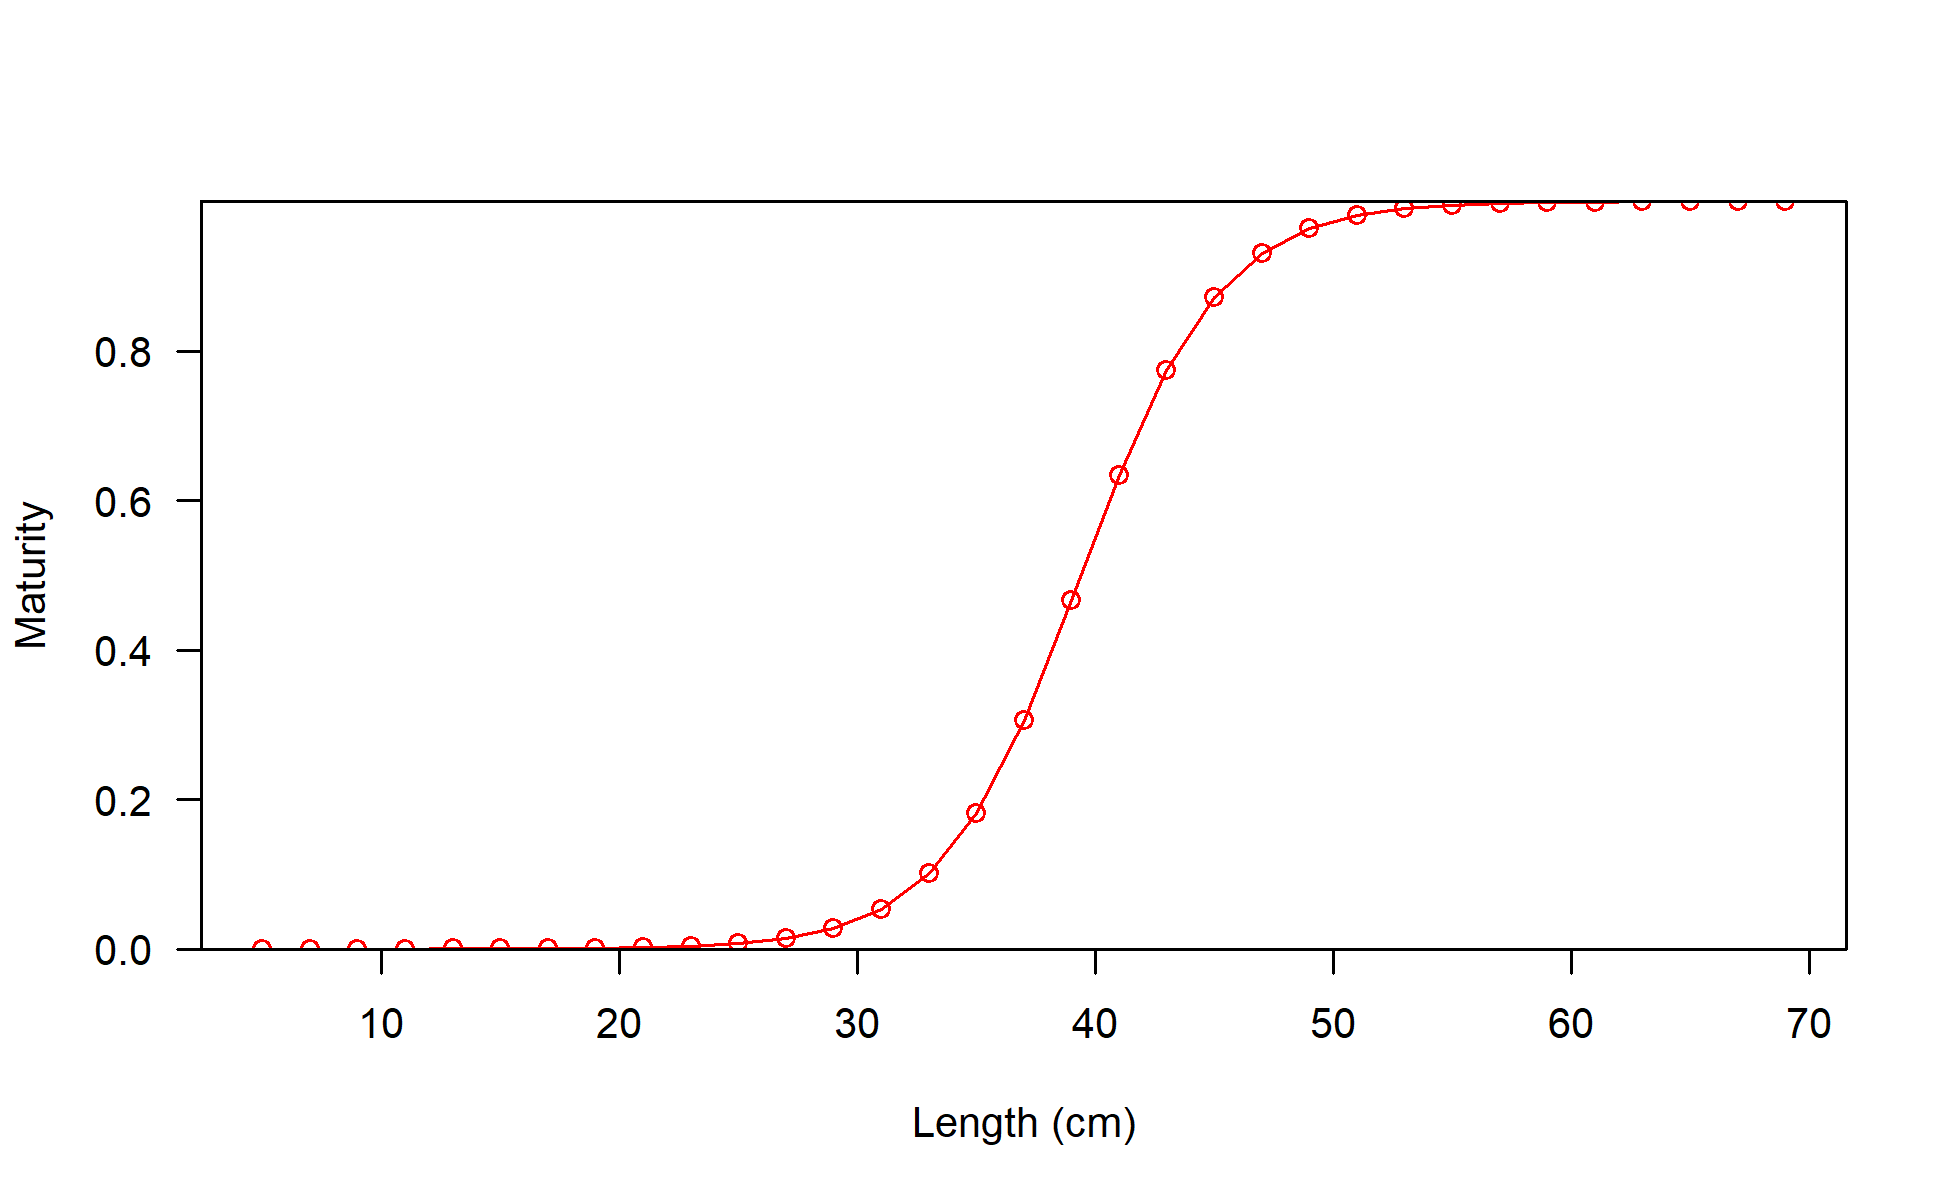
\includegraphics[width=1\textwidth,height=1\textheight]{C:/Users/Jason.Cope/Documents/Github/Vermilion rockfish OR WA assessment 2021/OR/write_up/models/Reference model/plots/bio6_maturity.png}
\caption{Maturity as a function of length.\label{fig:maturity}}
\end{figure}

\tagmcend\tagstructend

\tagstructbegin{tag=Figure,alttext={Fecundity as a function of length.}}\tagmcbegin{tag=Figure}

\begin{figure}
\centering
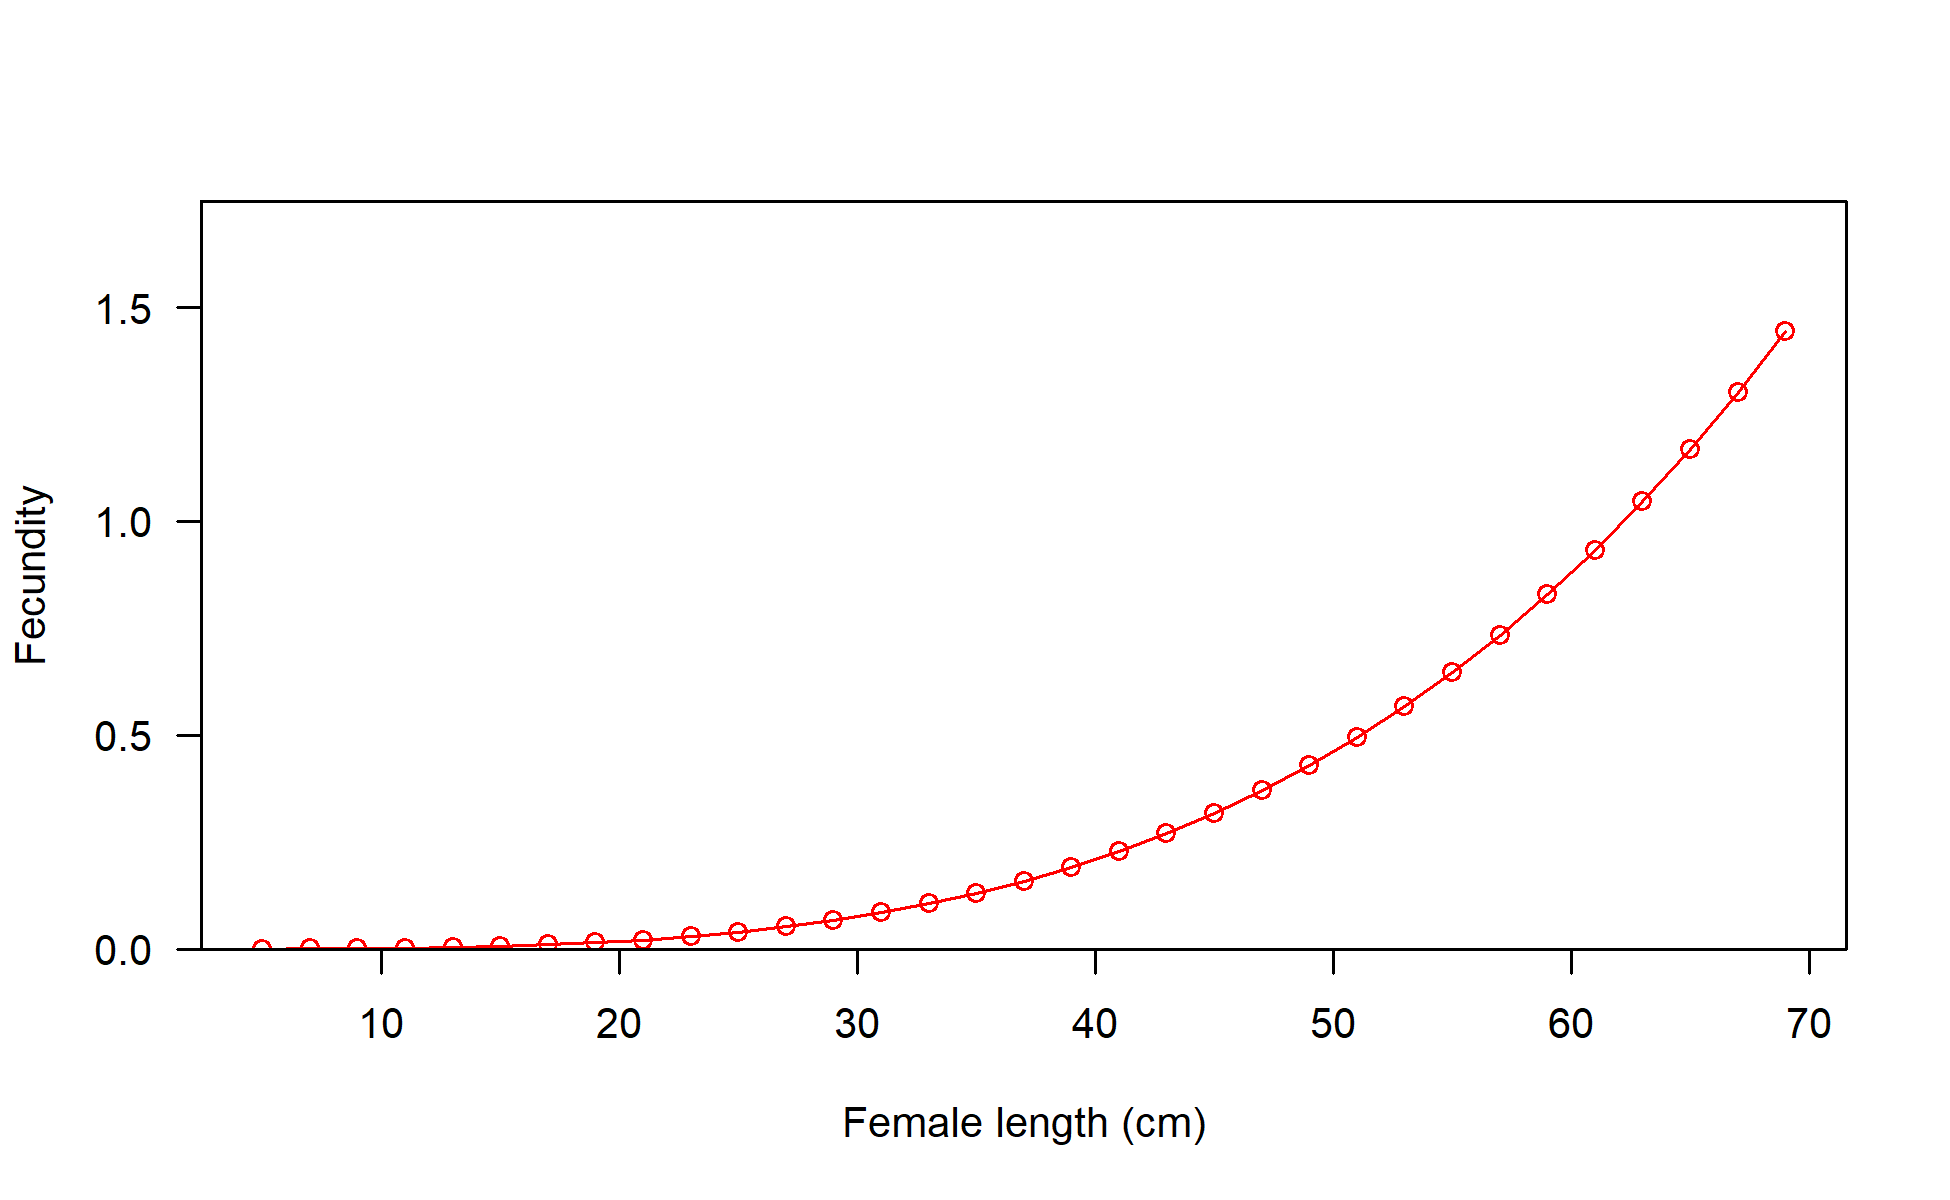
\includegraphics[width=1\textwidth,height=1\textheight]{C:/Users/Jason.Cope/Documents/Github/Vermilion rockfish OR WA assessment 2021/OR/write_up/models/Reference model/plots/bio9_fecundity_len.png}
\caption{Fecundity as a function of length.\label{fig:fecundity}}
\end{figure}

\tagmcend\tagstructend

\tagstructbegin{tag=Figure,alttext={Composite natural mortality distriubtion for $S. hopkinsi$ using four longevity estimators each with a SD = 0.2 presuming a lognomral error distibution.}}\tagmcbegin{tag=Figure}

\begin{figure}
\centering
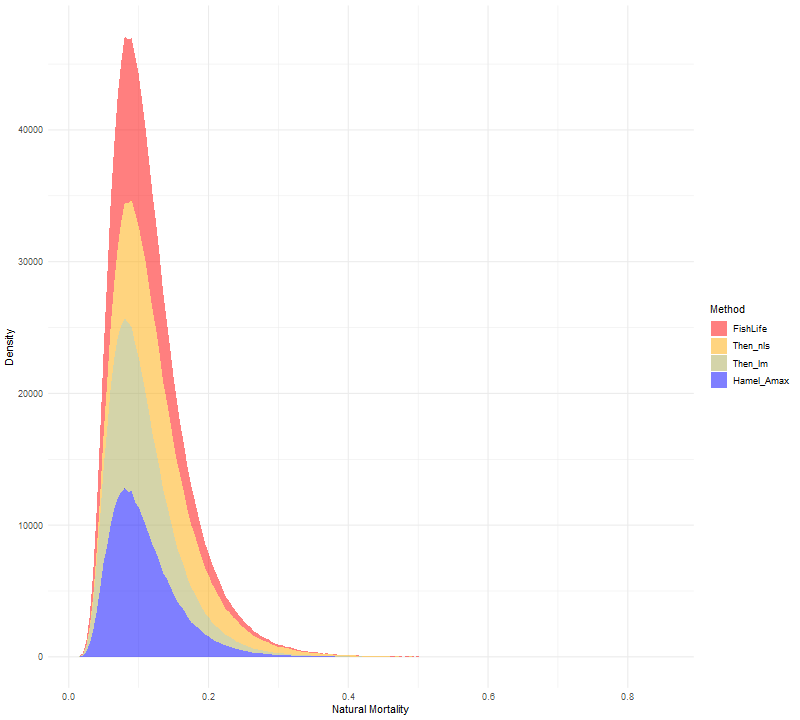
\includegraphics[width=1\textwidth,height=1\textheight]{C:/Users/Jason.Cope/Documents/Github/Vermilion rockfish OR WA assessment 2021/OR/write_up/figures/biology_plots/Mdensityplots_OR_vermilion.png}
\caption{Composite natural mortality distriubtion for {\tagstructbegin{tag=Formula}\tagmcbegin{tag=Formula}\(S. hopkinsi\)\leavevmode\tagmcend\tagstructend} using four longevity estimators each with a SD = 0.2 presuming a lognomral error distibution.\label{fig:M_composite_dists}}
\end{figure}

\tagmcend\tagstructend

\tagstructbegin{tag=Figure,alttext={Length-weight data and fits to commercially-derived sex-specific vermilion samples.}}\tagmcbegin{tag=Figure}

\begin{figure}
\centering
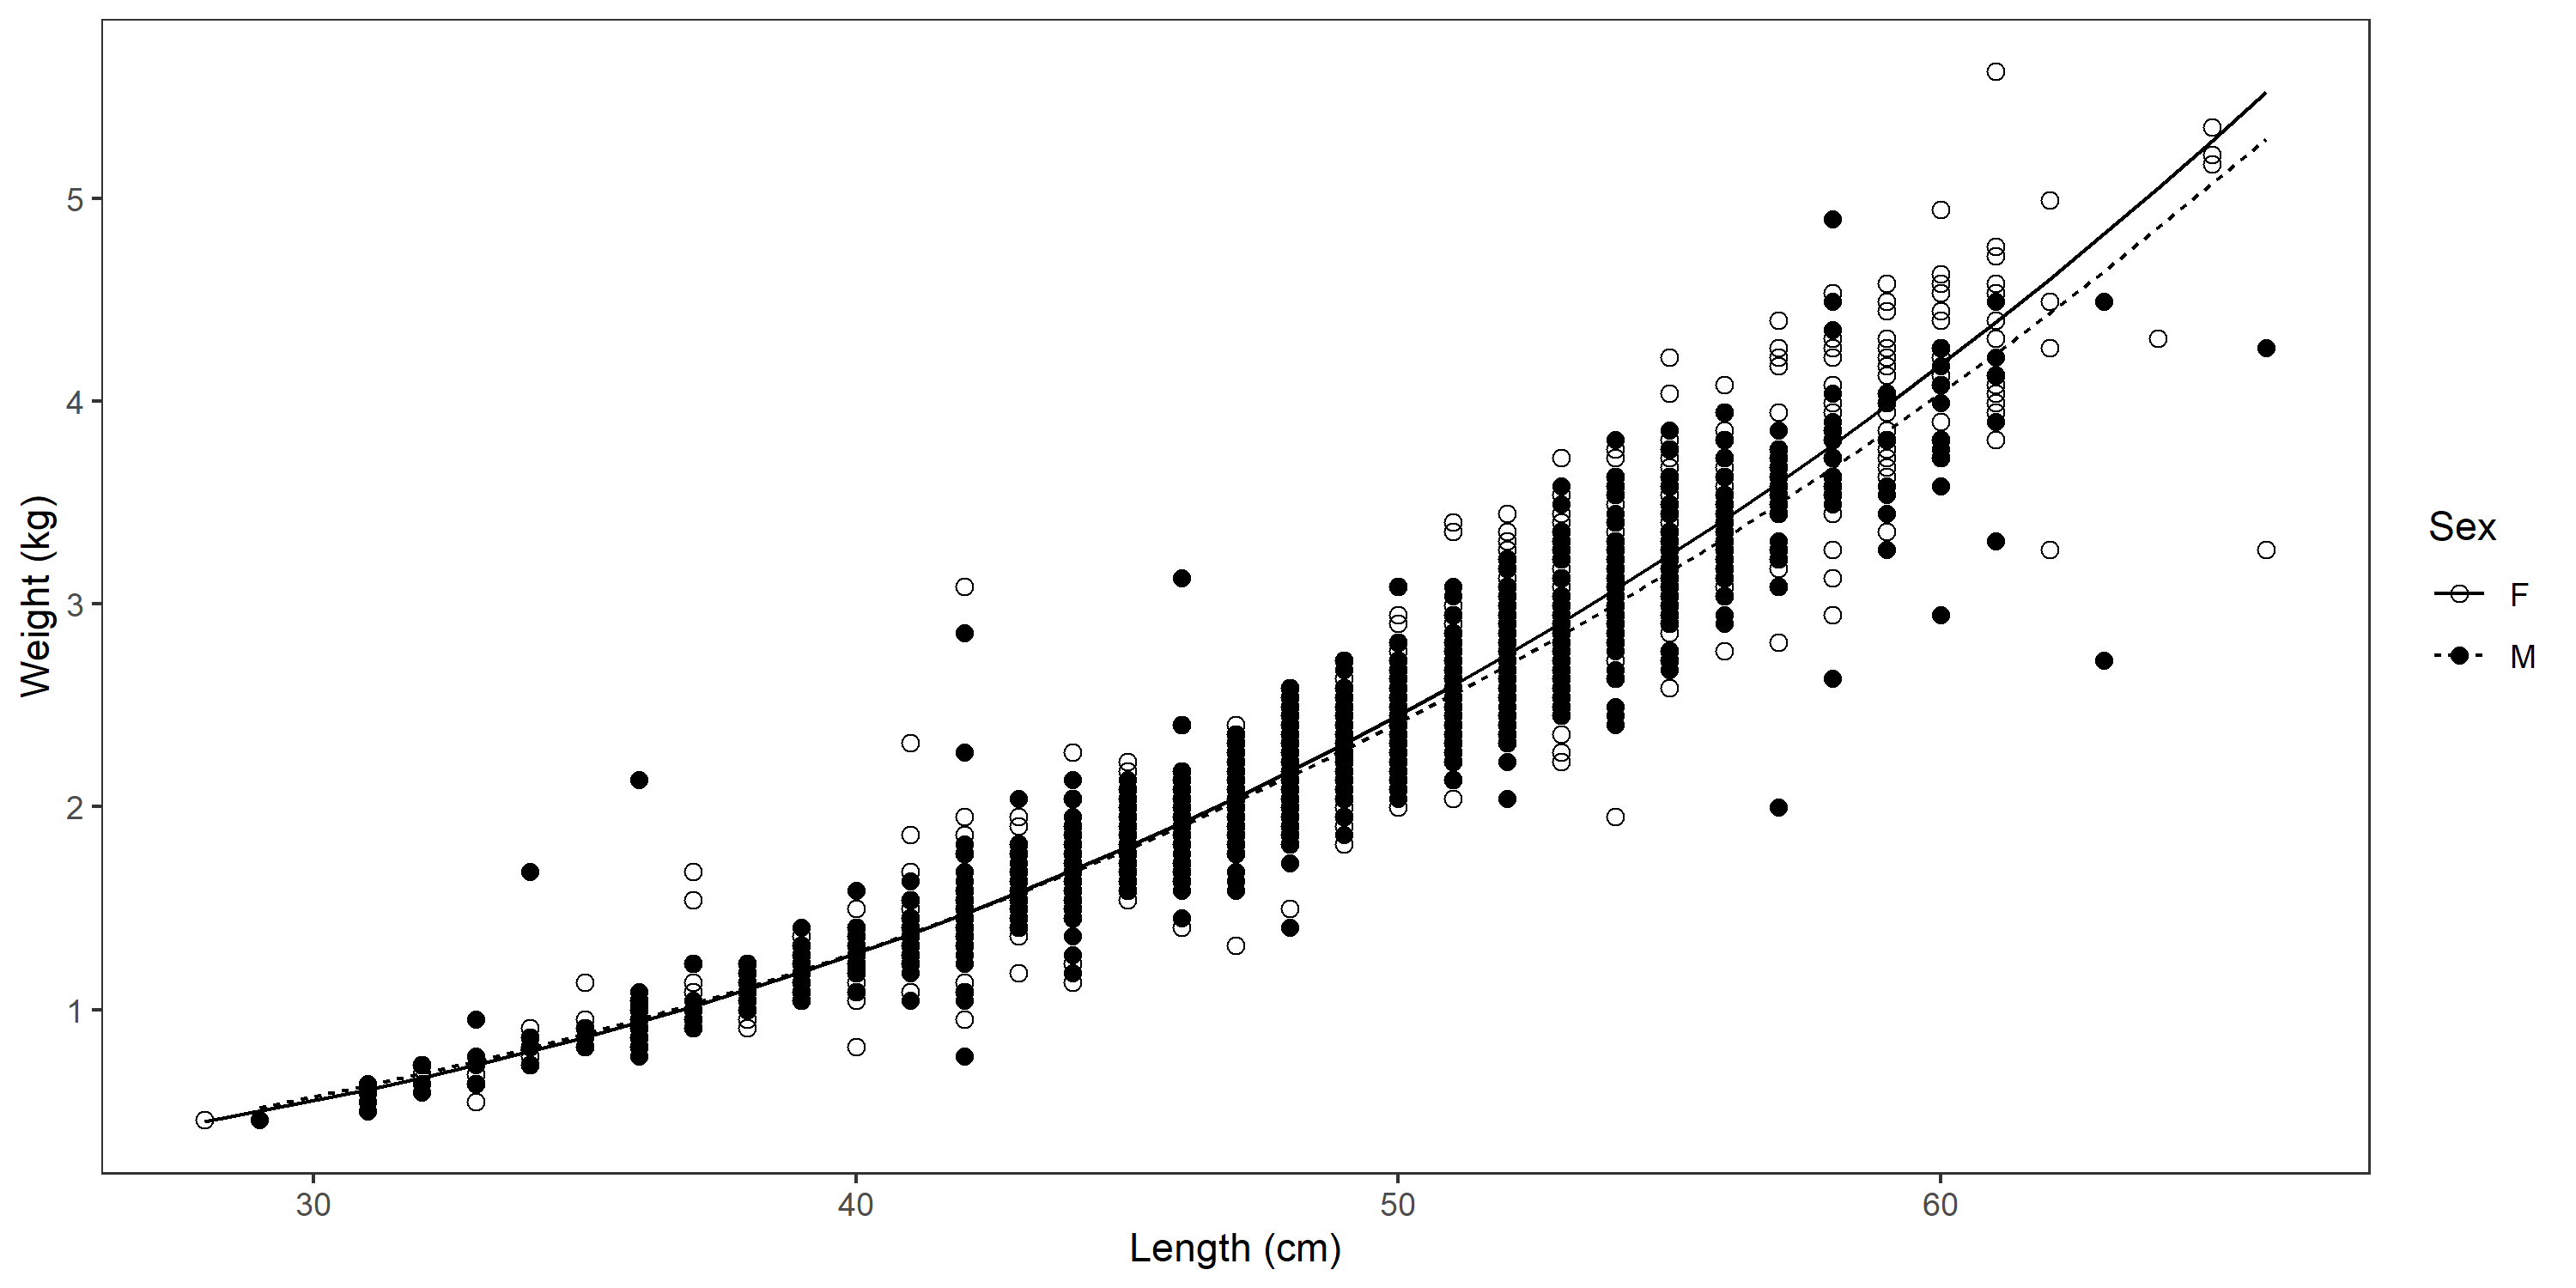
\includegraphics[width=1\textwidth,height=1\textheight]{C:/Users/Jason.Cope/Documents/Github/Vermilion rockfish OR WA assessment 2021/OR/write_up/figures/biology_plots/OR_Vermilion_Sexed Length vs Weight_withpower.png}
\caption{Length-weight data and fits to commercially-derived sex-specific vermilion samples.\label{fig:len-weight-fit}}
\end{figure}

\tagmcend\tagstructend

\tagstructbegin{tag=Figure,alttext={Selectivity at length by fleet.}}\tagmcbegin{tag=Figure}

\begin{figure}
\centering
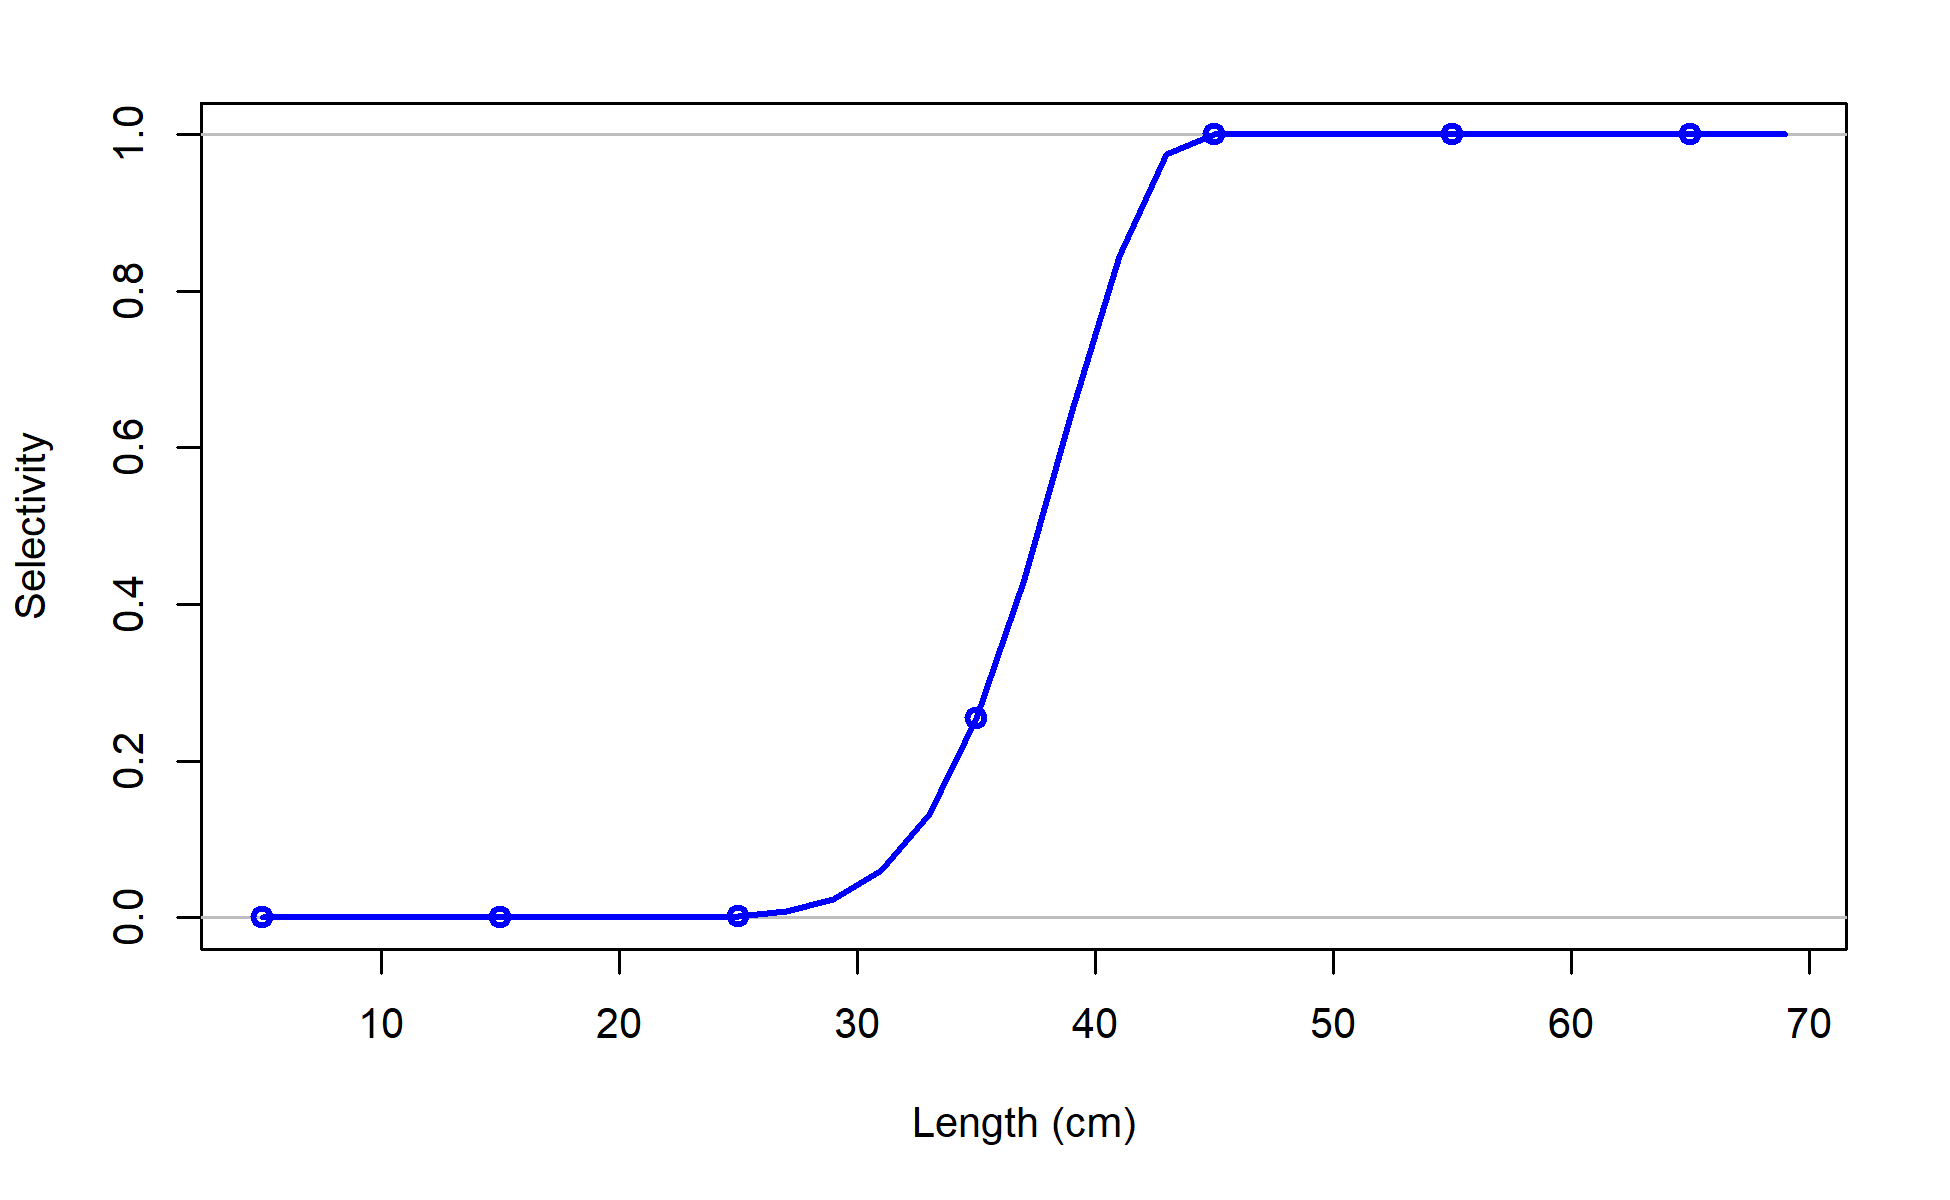
\includegraphics[width=1\textwidth,height=1\textheight]{C:/Users/Jason.Cope/Documents/Github/Vermilion rockfish OR WA assessment 2021/OR/write_up/models/Reference model/plots/sel01_multiple_fleets_length1.png}
\caption{Selectivity at length by fleet.\label{fig:selex}}
\end{figure}

\tagmcend\tagstructend

\tagstructbegin{tag=Figure,alttext={Jitter runs for the squarespot rockfish reference model, with jitter run number on the x-axis and -log likelihood value on the y-axis. Blue dot are models that match the likelihood value of the reference model, while red dots deviate from the reference model. All red dots are above the blue dots, indicating no better fit to the reference model was found.}}\tagmcbegin{tag=Figure}

\begin{figure}
\centering
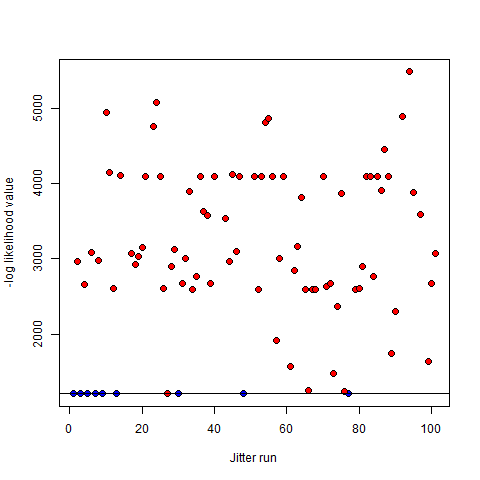
\includegraphics[width=1\textwidth,height=1\textheight]{C:/Users/Jason.Cope/Documents/Github/Vermilion rockfish OR WA assessment 2021/OR/write_up/models/Reference model/Jitter Results/jitterplot_01.png}
\caption{Jitter runs for the squarespot rockfish reference model, with jitter run number on the x-axis and -log likelihood value on the y-axis. Blue dot are models that match the likelihood value of the reference model, while red dots deviate from the reference model. All red dots are above the blue dots, indicating no better fit to the reference model was found.\label{fig:jitter_01}}
\end{figure}

\tagmcend\tagstructend

\tagstructbegin{tag=Figure,alttext={Pearson residuals for the commercial (top panel) and recreational (bottom panel) fleet. Closed bubble are positive residuals (observed > expected) and open bubbles are negative residuals (observed < expected).}}\tagmcbegin{tag=Figure}

\begin{figure}
\centering
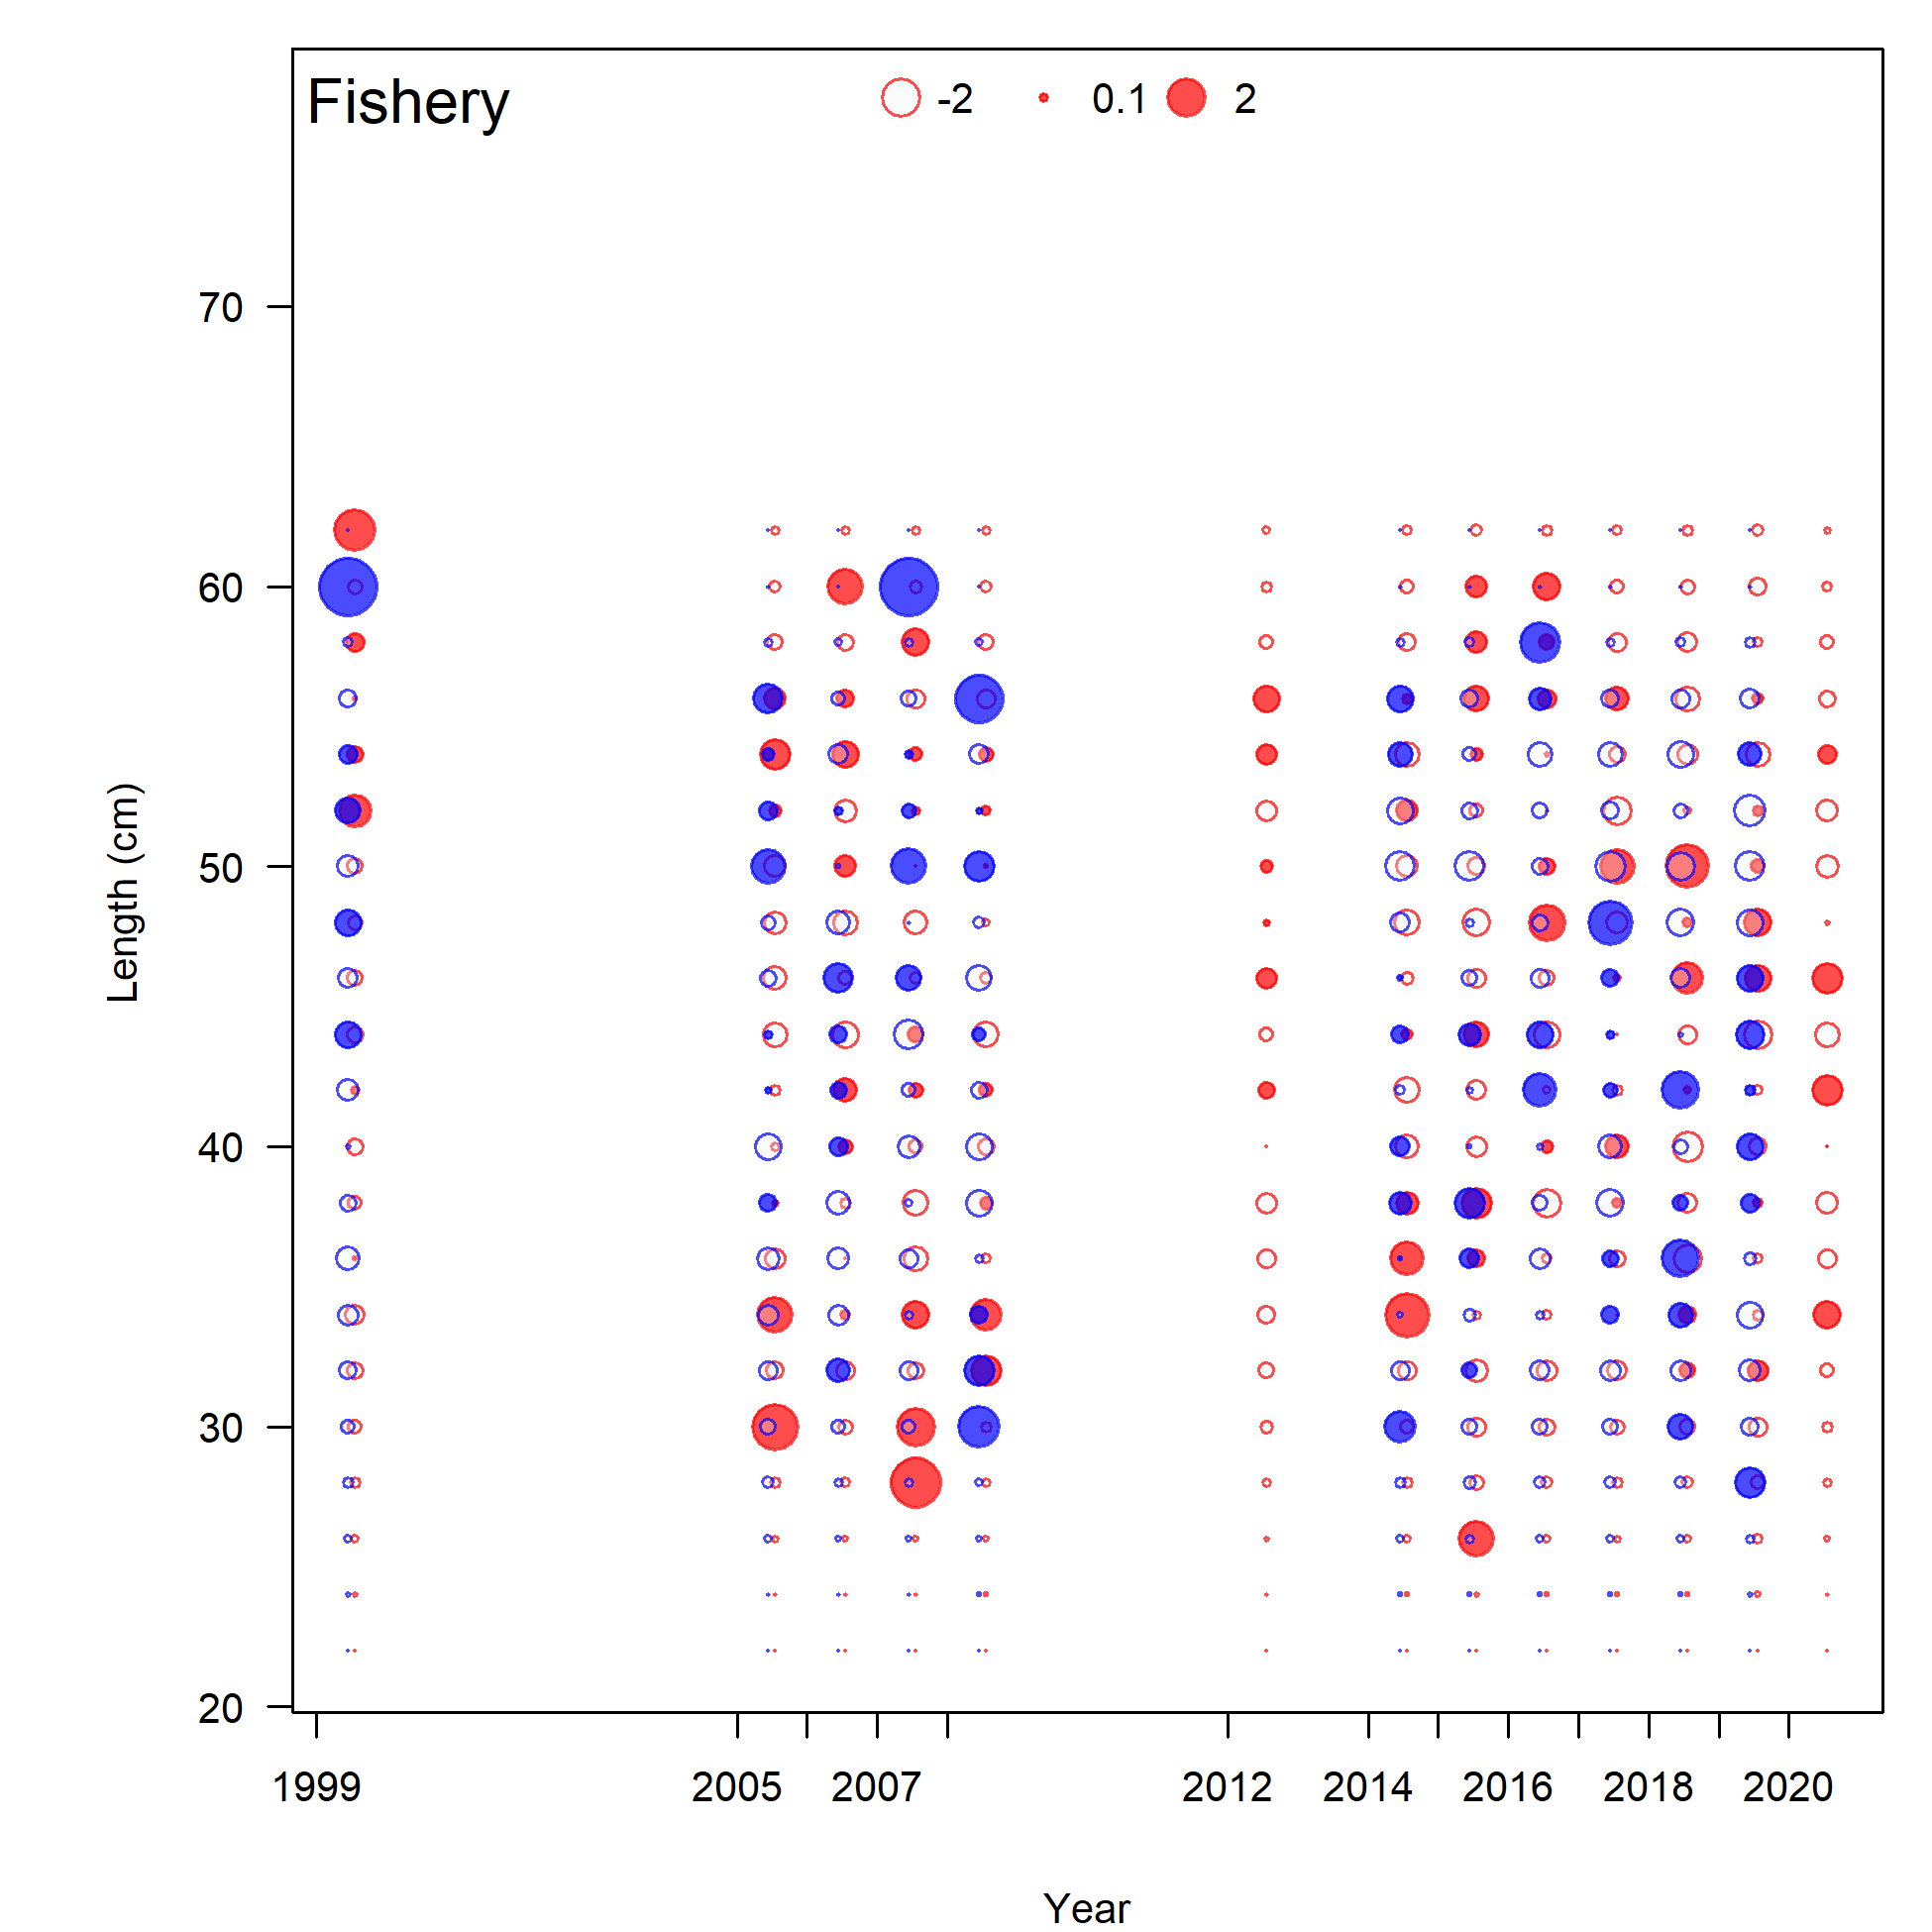
\includegraphics[width=1\textwidth,height=1\textheight]{C:/Users/Jason.Cope/Documents/Github/Vermilion rockfish OR WA assessment 2021/OR/write_up/models/Reference model/plots/comp_lenfit__multi-fleet_comparison.png}
\caption{Pearson residuals for the commercial (top panel) and recreational (bottom panel) fleet. Closed bubble are positive residuals (observed \textgreater{} expected) and open bubbles are negative residuals (observed \textless{} expected).\label{fig:com-rec-pearson}}
\end{figure}

\tagmcend\tagstructend

\tagstructbegin{tag=Figure,alttext={Mean length index from the commercial fishery with 95 percent confidence intervals based on sample sizes and data weighting.}}\tagmcbegin{tag=Figure}

\begin{figure}
\centering
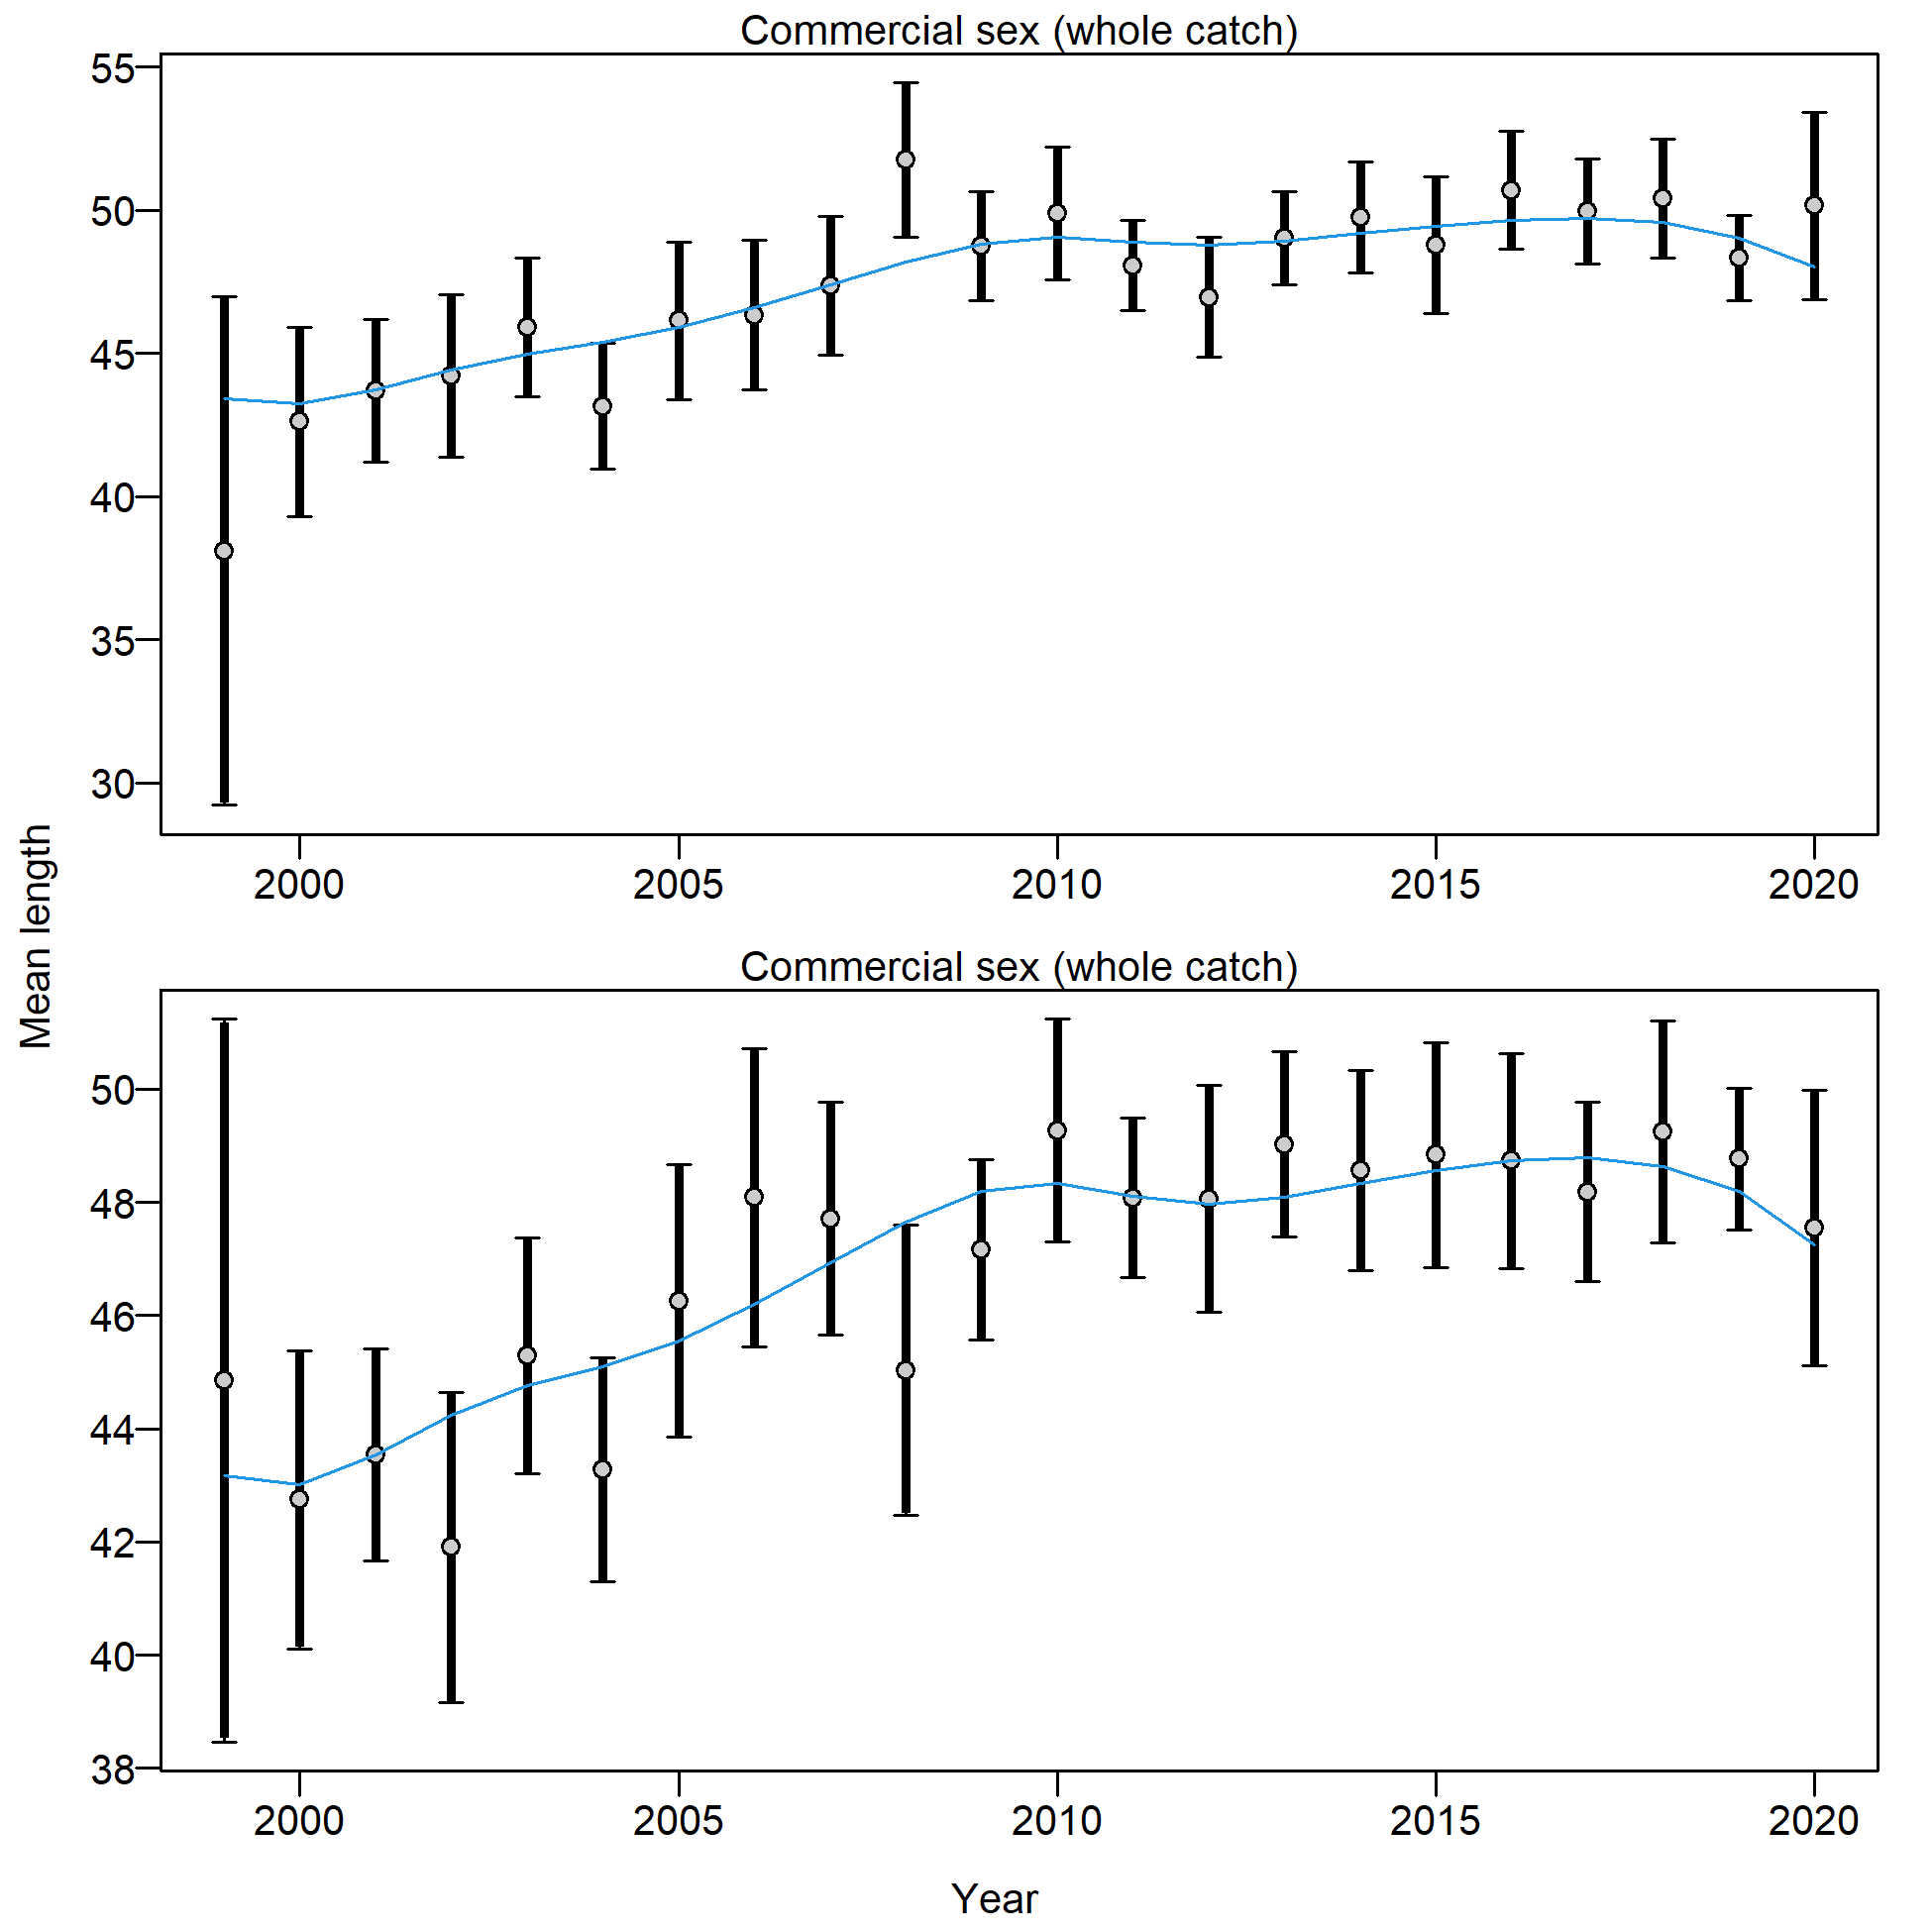
\includegraphics[width=1\textwidth,height=1\textheight]{C:/Users/Jason.Cope/Documents/Github/Vermilion rockfish OR WA assessment 2021/OR/write_up/models/Reference model/plots/comp_lenfit_data_weighting_TA1.8_Commercial_fit.png}
\caption{Mean length index from the commercial fishery with 95 percent confidence intervals based on sample sizes and data weighting.\label{fig:com-mean-len-fit}}
\end{figure}

\tagmcend\tagstructend

\tagstructbegin{tag=Figure,alttext={Mean length index from the recreational fishery with 95 percent confidence intervals based on sample sizes and data weighting.}}\tagmcbegin{tag=Figure}

\begin{figure}
\centering
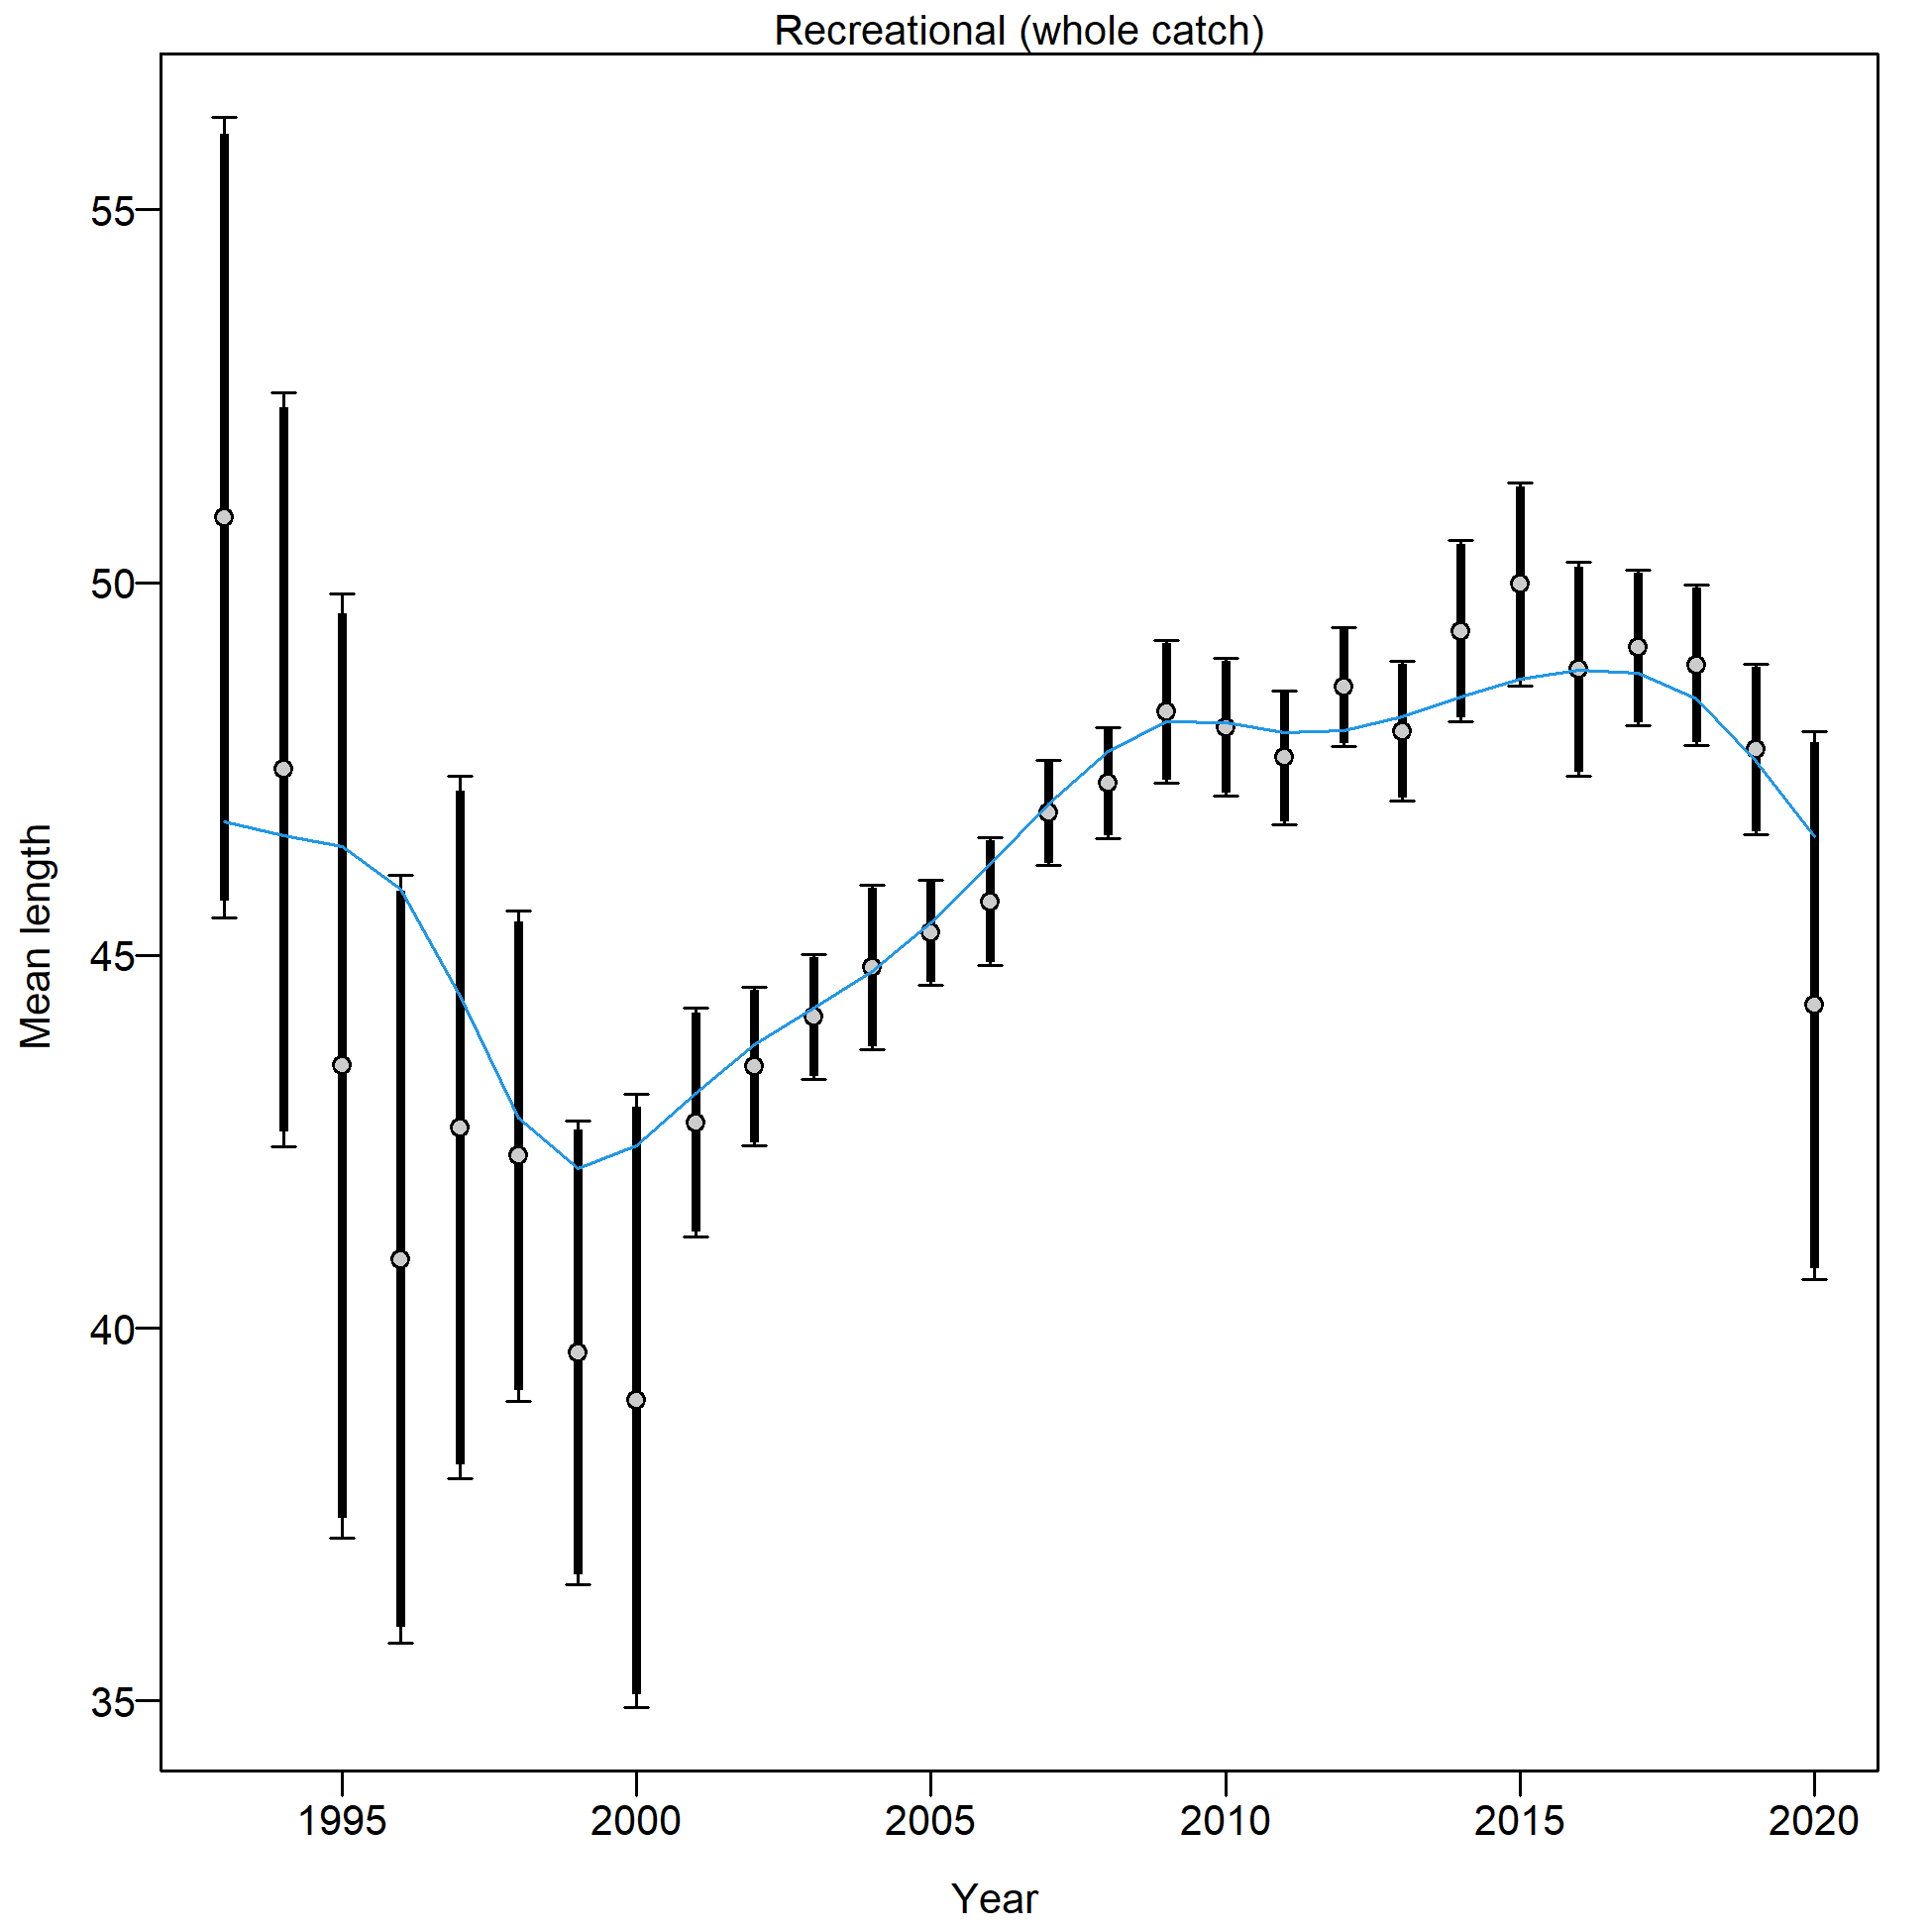
\includegraphics[width=1\textwidth,height=1\textheight]{C:/Users/Jason.Cope/Documents/Github/Vermilion rockfish OR WA assessment 2021/OR/write_up/models/Reference model/plots/comp_lenfit_data_weighting_TA1.8_Recreational_fit.png}
\caption{Mean length index from the recreational fishery with 95 percent confidence intervals based on sample sizes and data weighting.\label{fig:rec-mean-len-fit}}
\end{figure}

\tagmcend\tagstructend

\tagstructbegin{tag=Figure,alttext={Aggregated length comps over all years.}}\tagmcbegin{tag=Figure}

\begin{figure}
\centering
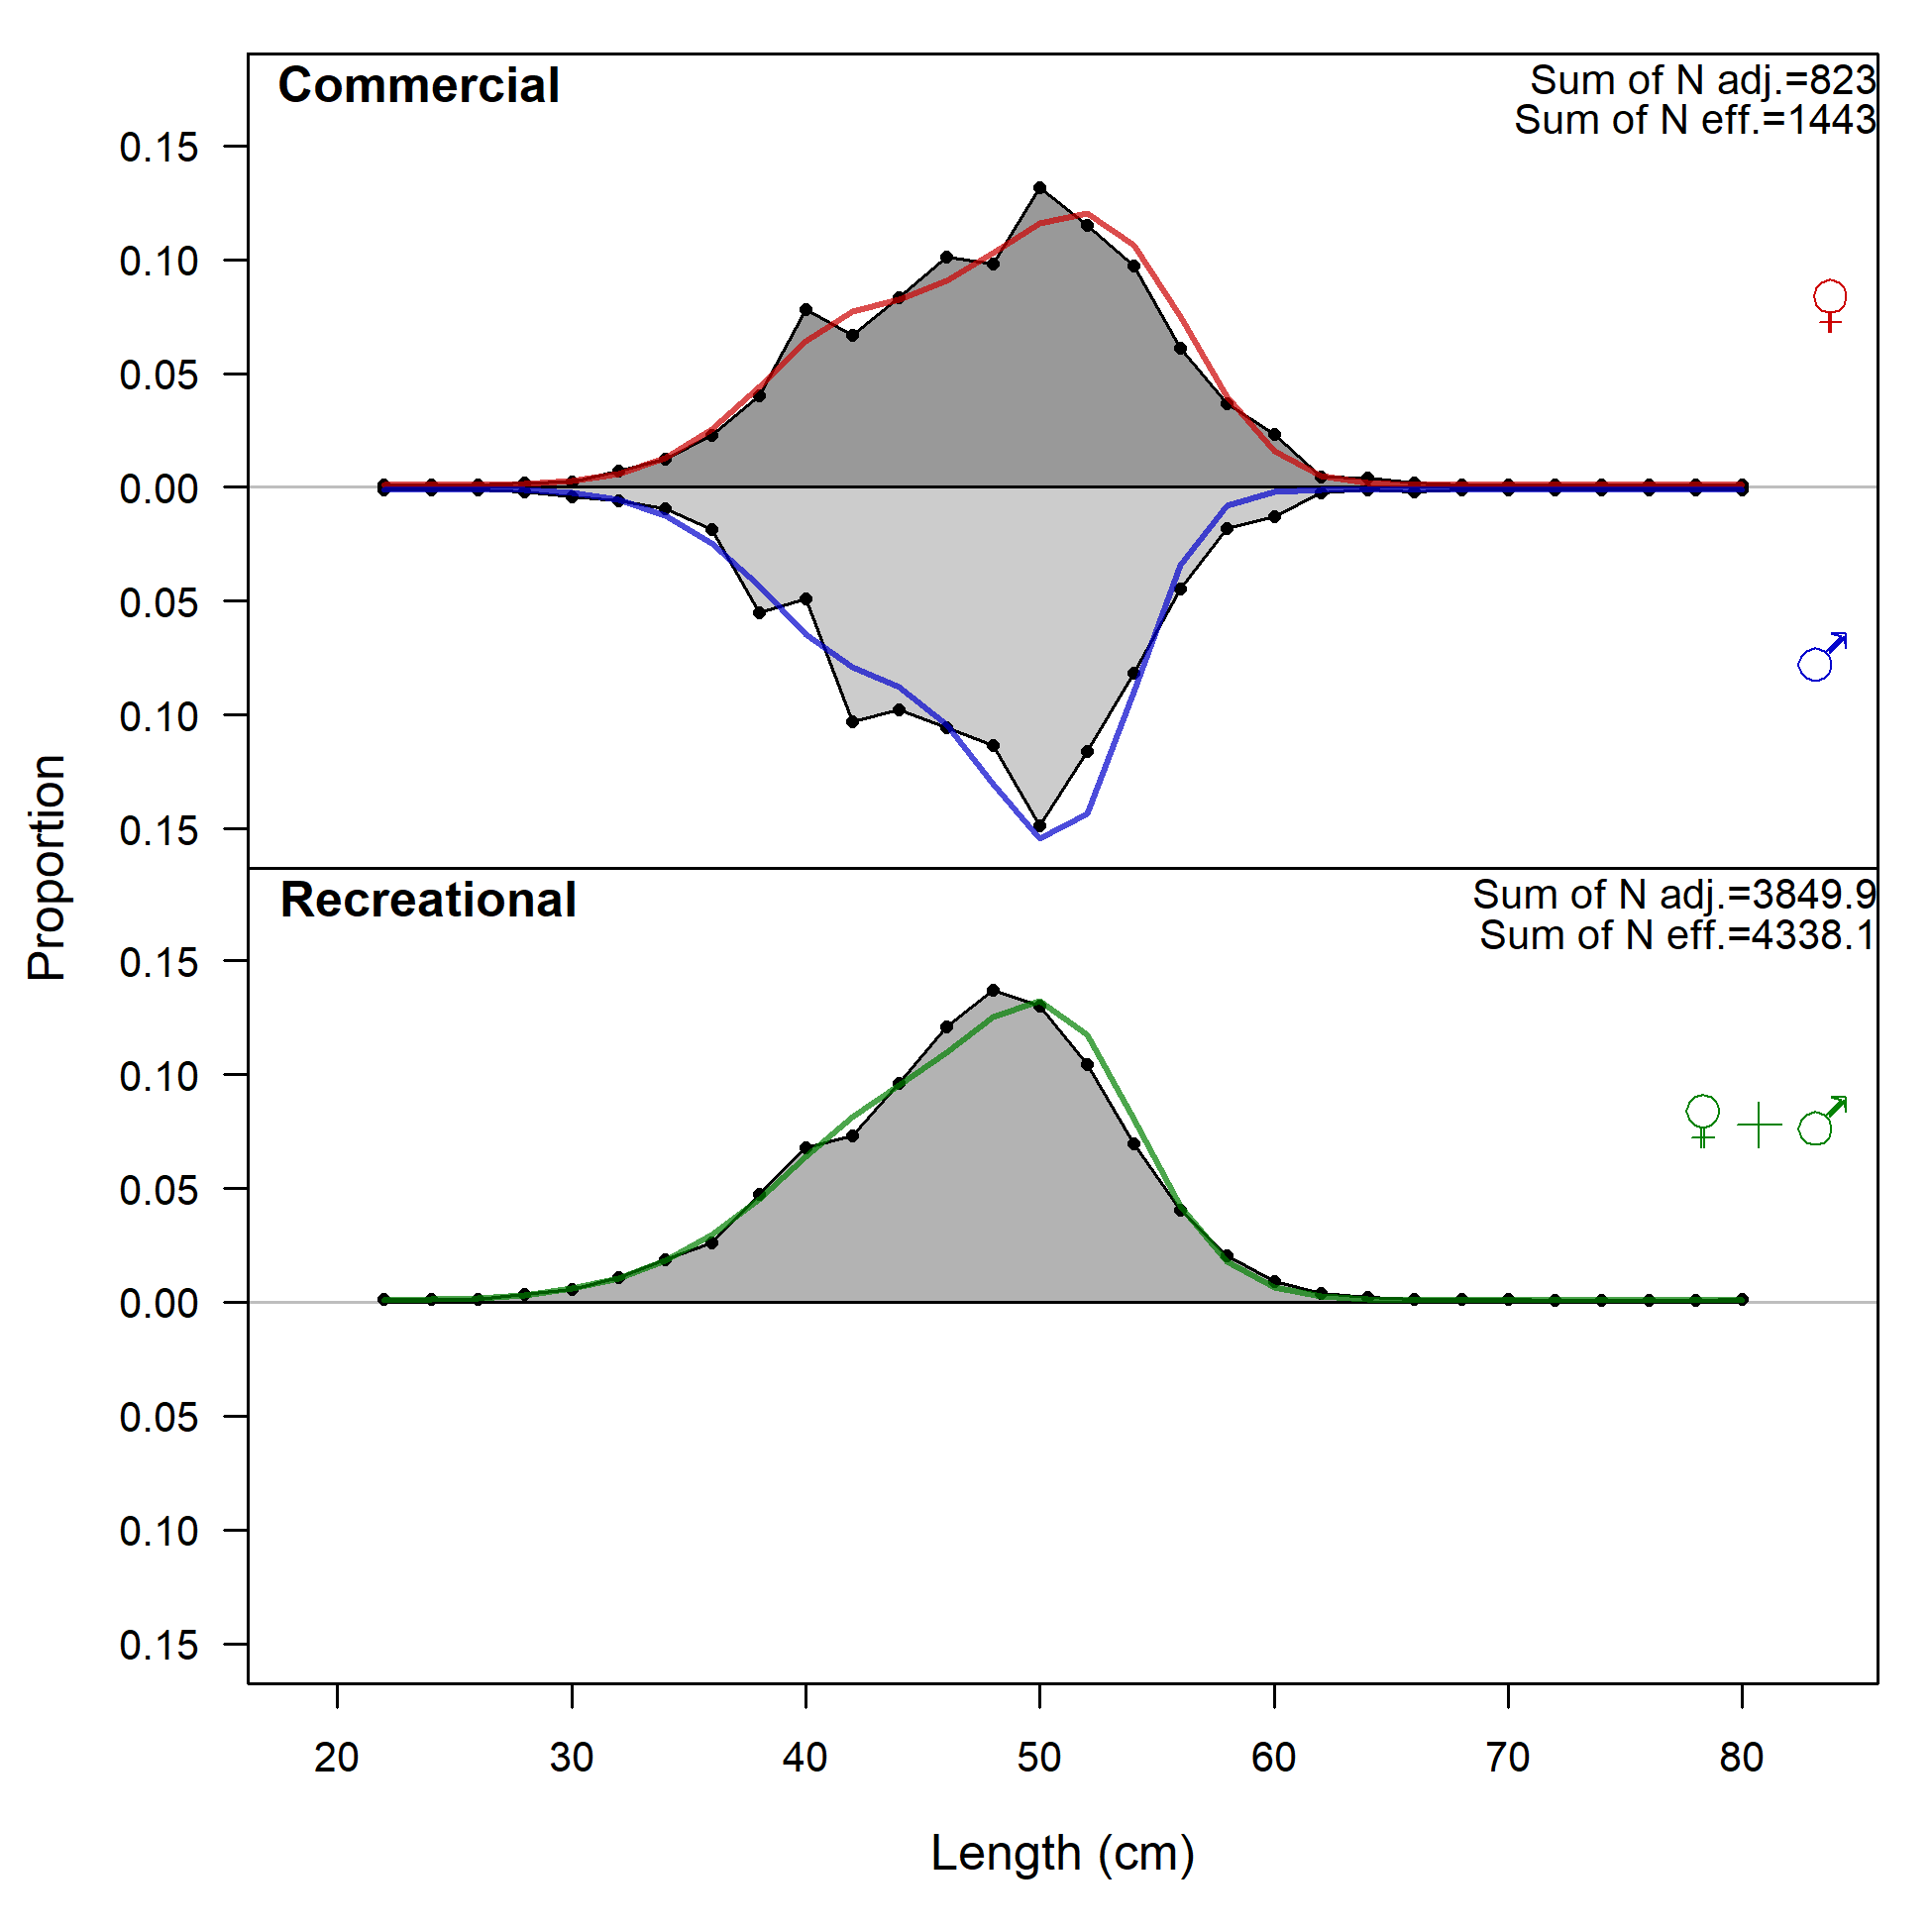
\includegraphics[width=1\textwidth,height=1\textheight]{C:/Users/Jason.Cope/Documents/Github/Vermilion rockfish OR WA assessment 2021/OR/write_up/models/Reference model/plots/comp_lenfit__aggregated_across_time.png}
\caption{Aggregated length comps over all years.\label{fig:agg-len-fit}}
\end{figure}

\tagmcend\tagstructend

\tagstructbegin{tag=Figure,alttext={Mean age from conditional age-at-length data for the Commercial.}}\tagmcbegin{tag=Figure}

\begin{figure}
\centering
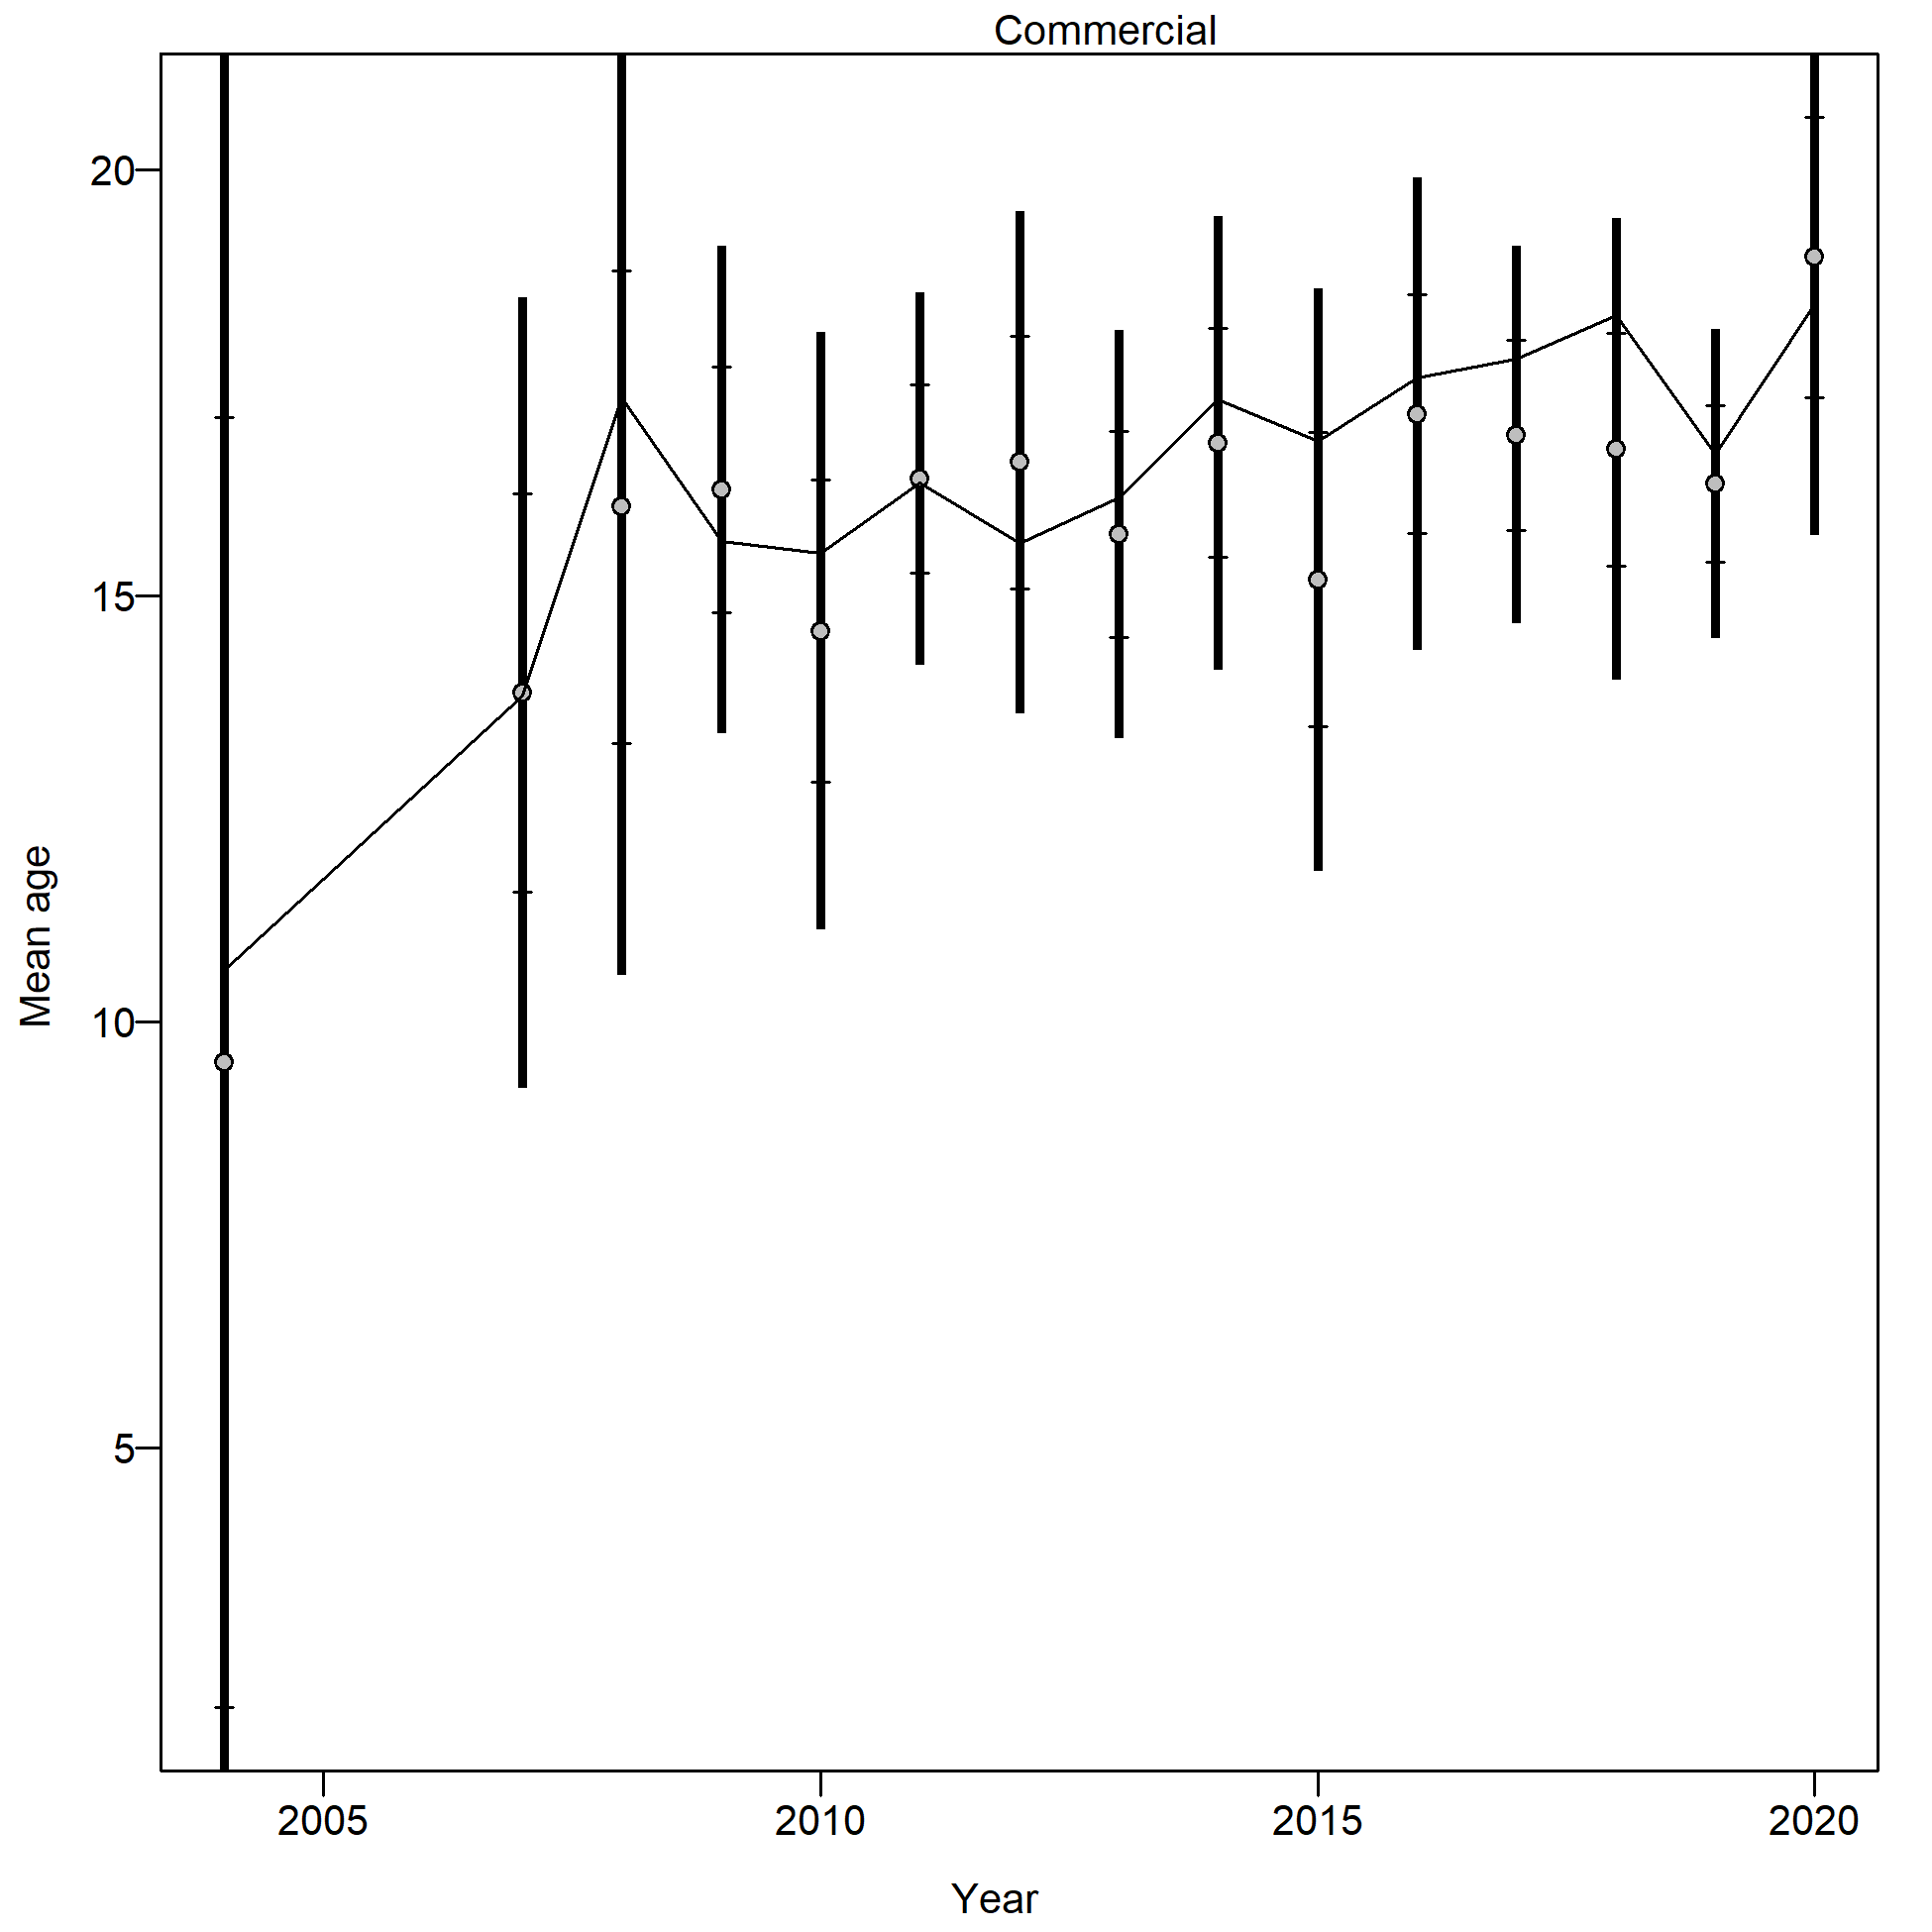
\includegraphics[width=1\textwidth,height=1\textheight]{C:/Users/Jason.Cope/Documents/Github/Vermilion rockfish OR WA assessment 2021/OR/write_up/models/Reference model/plots/comp_condAALfit_data_weighting_TA1.8_condAgeCommercial_fit.png}
\caption{Mean age from conditional age-at-length data for the Commercial.\label{fig:com-mean-caal}}
\end{figure}

\tagmcend\tagstructend

\tagstructbegin{tag=Figure,alttext={Mean age observations from the conditional age-at-length data from the Recreational fishery.}}\tagmcbegin{tag=Figure}

\begin{figure}
\centering
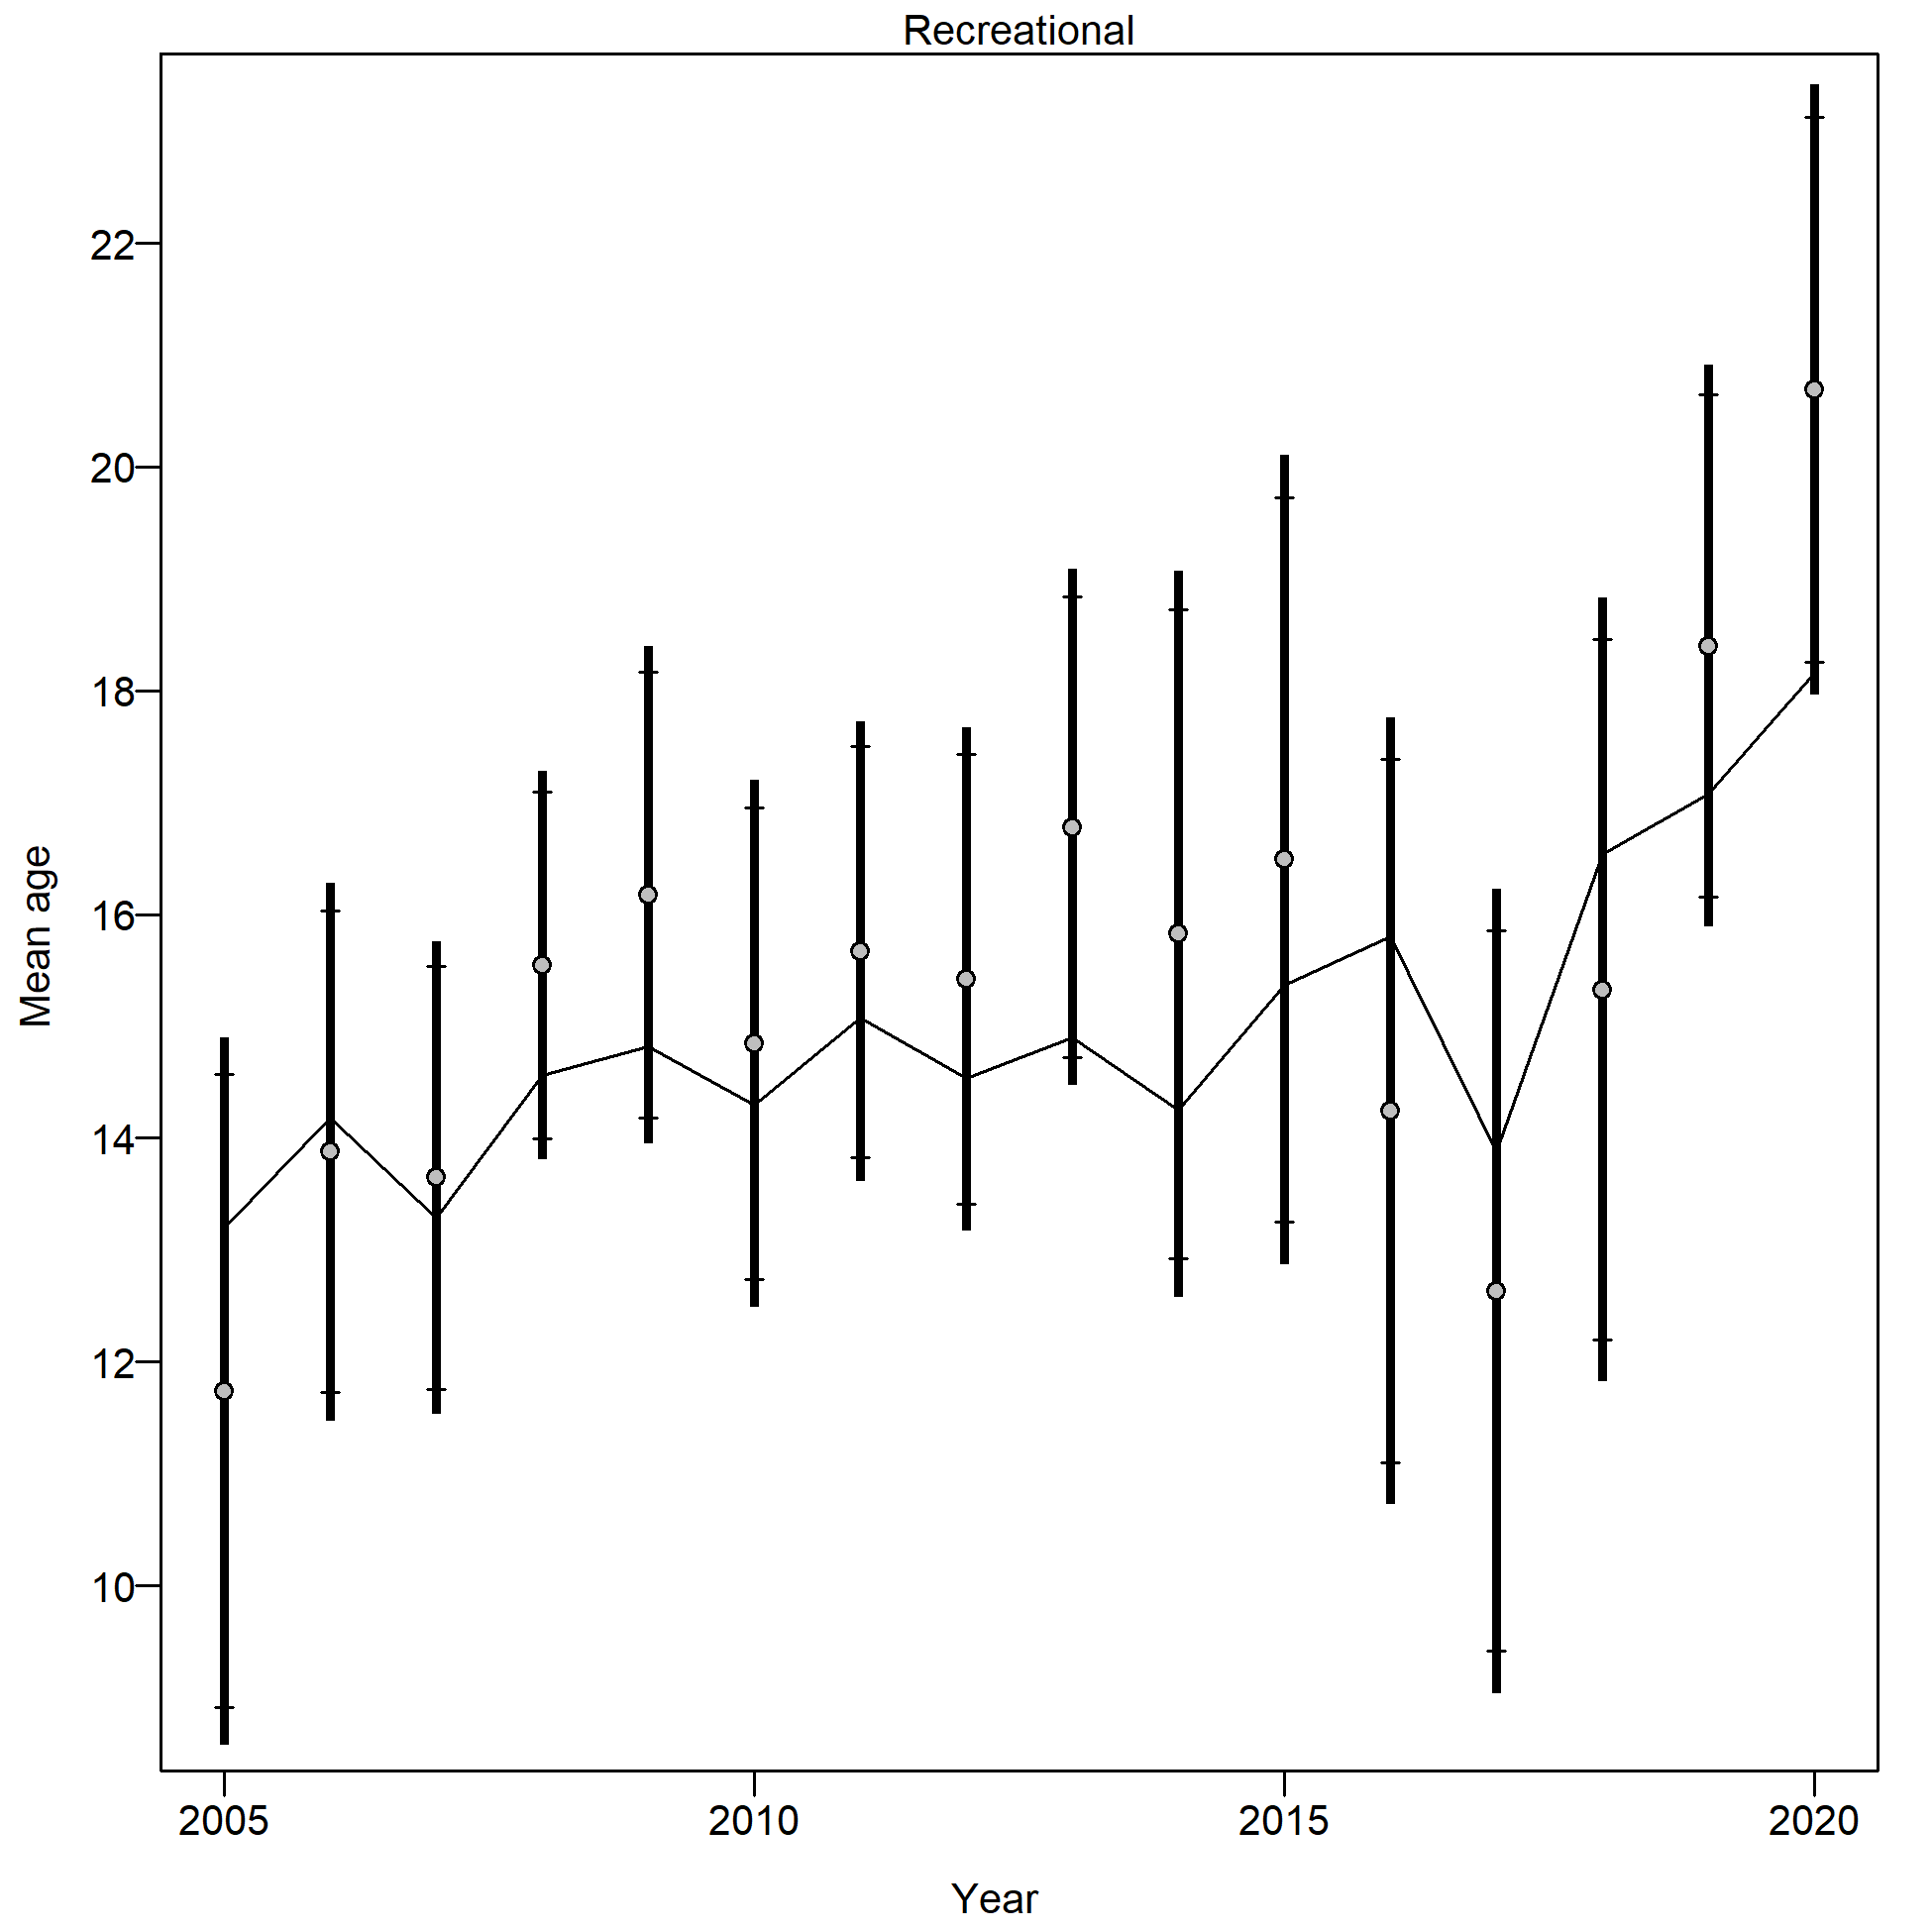
\includegraphics[width=1\textwidth,height=1\textheight]{C:/Users/Jason.Cope/Documents/Github/Vermilion rockfish OR WA assessment 2021/OR/write_up/models/Reference model/plots/comp_condAALfit_data_weighting_TA1.8_condAgeRecreational_fit.png}
\caption{Mean age observations from the conditional age-at-length data from the Recreational fishery.\label{fig:rec-mean-caal}}
\end{figure}

\tagmcend\tagstructend

\tagstructbegin{tag=Figure,alttext={Fit to the ORBS recreational survey index of abundance.}}\tagmcbegin{tag=Figure}

\begin{figure}
\centering
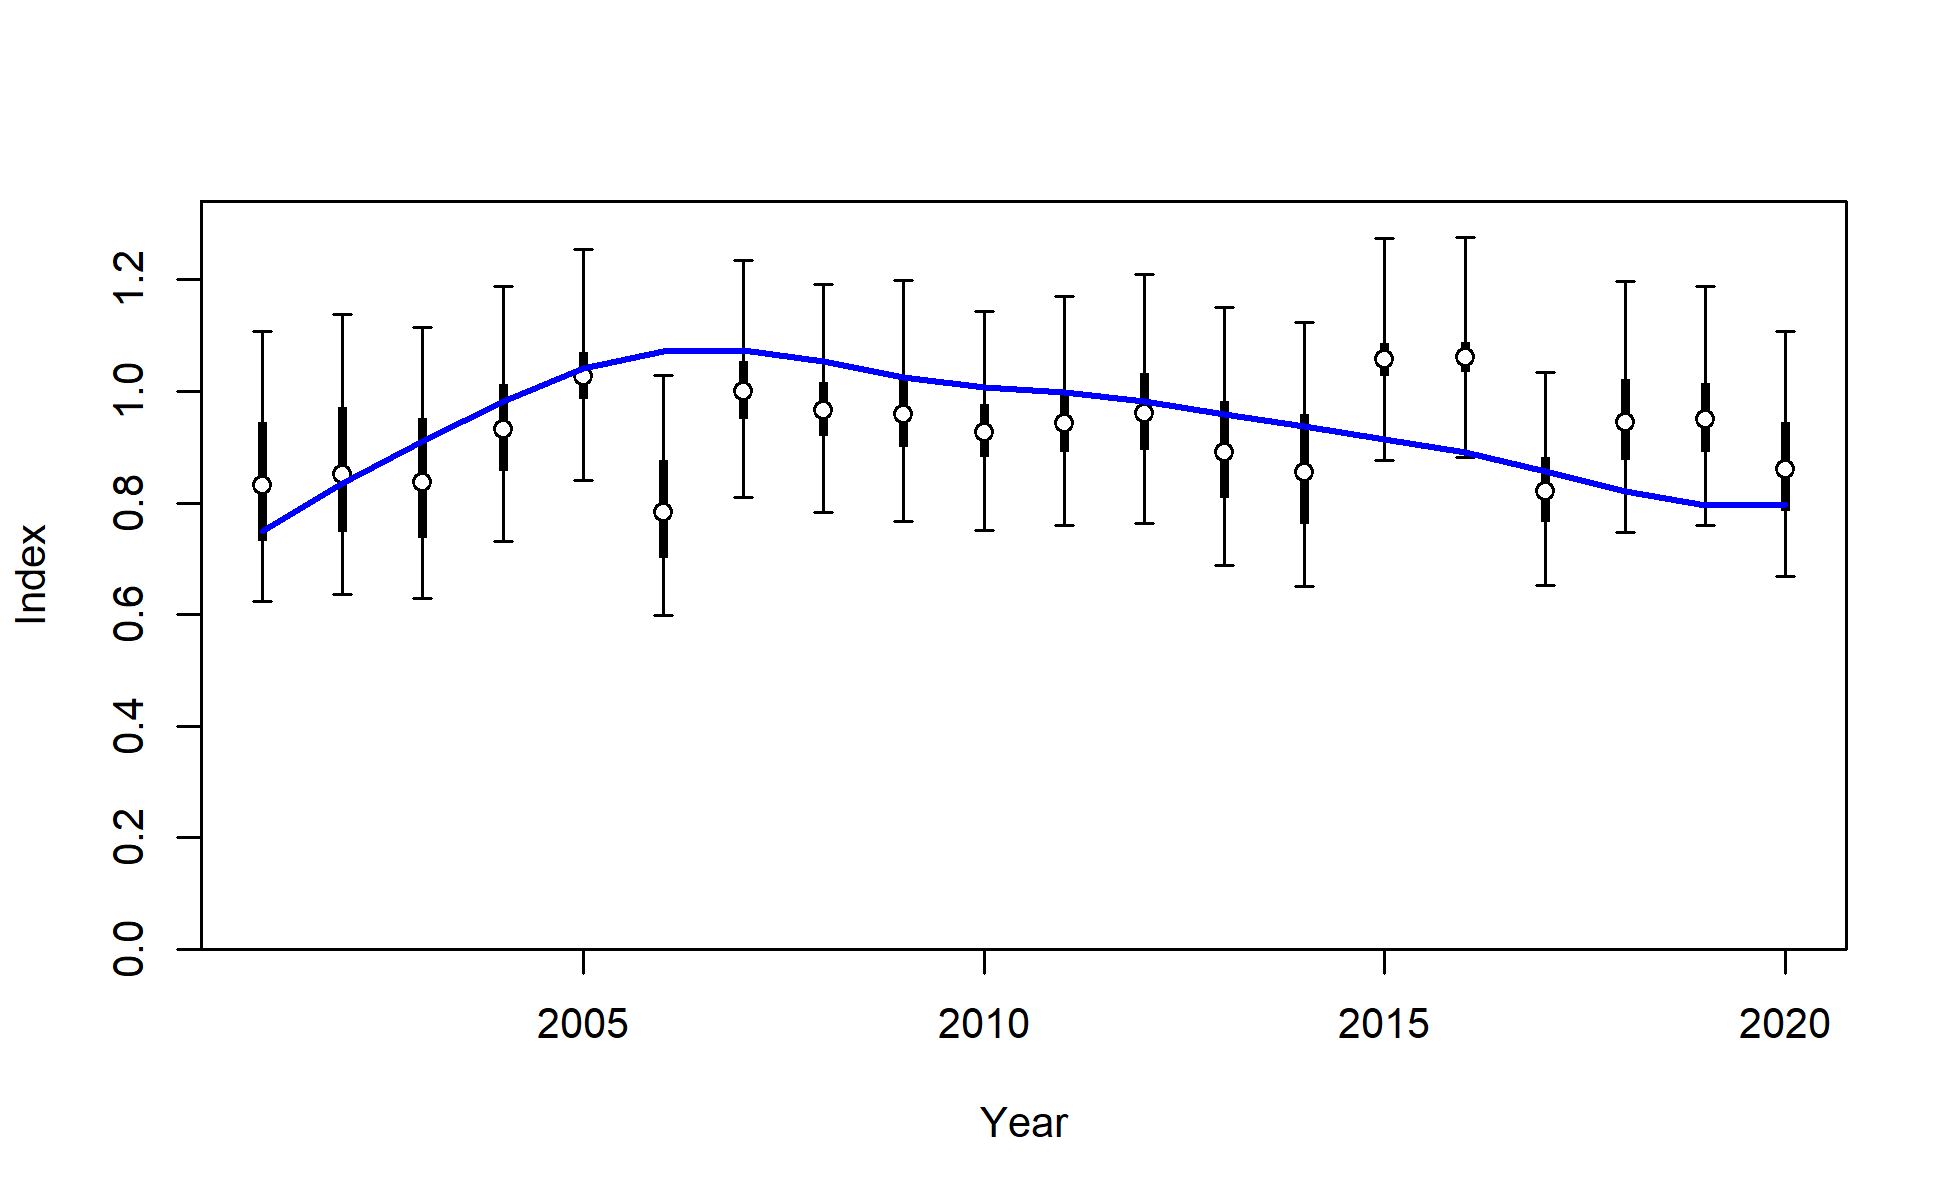
\includegraphics[width=1\textwidth,height=1\textheight]{C:/Users/Jason.Cope/Documents/Github/Vermilion rockfish OR WA assessment 2021/OR/write_up/models/Reference model/plots/index2_cpuefit_Recreational.png}
\caption{Fit to the ORBS recreational survey index of abundance.\label{fig:orbs-index-fit}}
\end{figure}

\tagmcend\tagstructend

\tagstructbegin{tag=Figure,alttext={Length-based selectivity curves for the commercial and recreational fisheries.}}\tagmcbegin{tag=Figure}

\begin{figure}
\centering
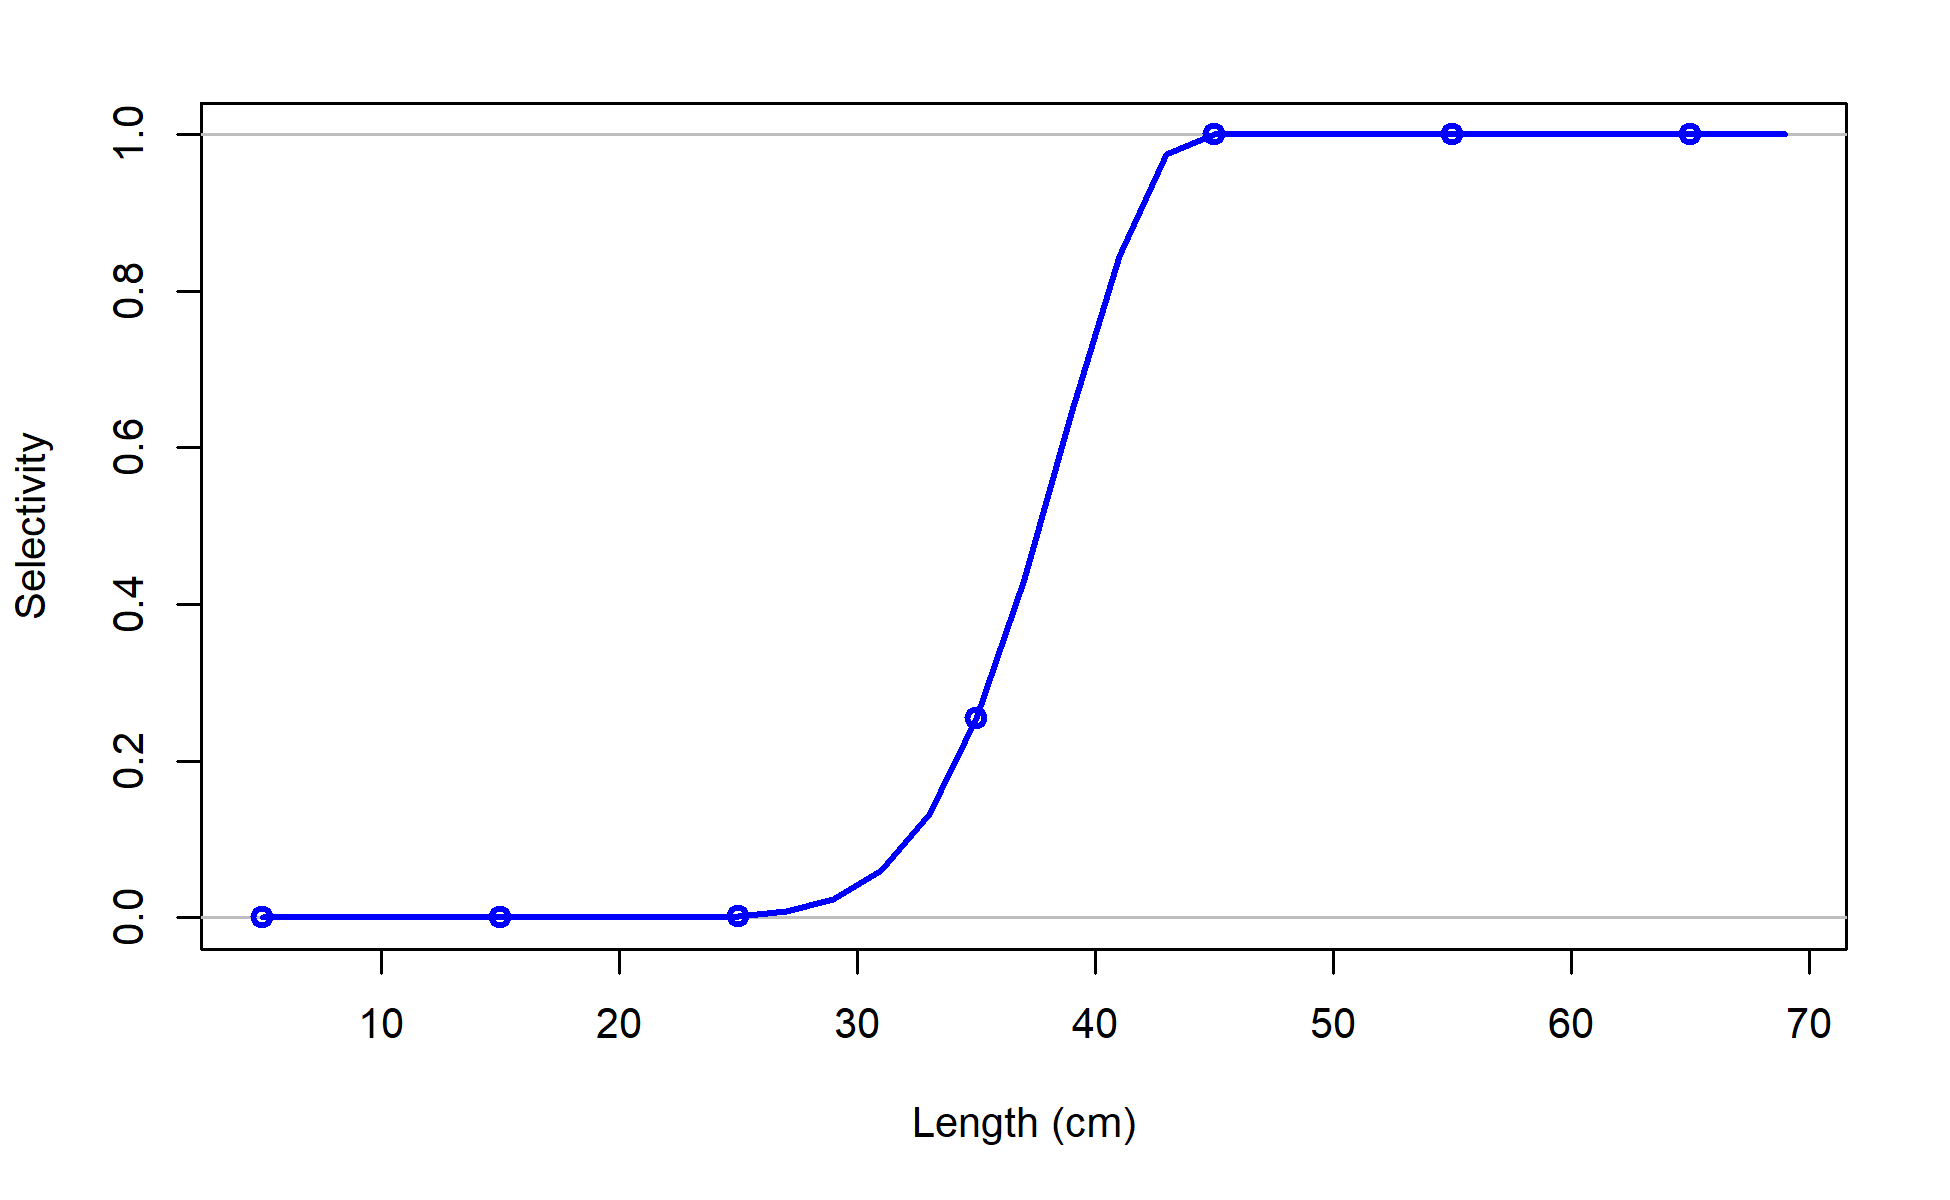
\includegraphics[width=1\textwidth,height=1\textheight]{C:/Users/Jason.Cope/Documents/Github/Vermilion rockfish OR WA assessment 2021/OR/write_up/models/Reference model/plots/sel01_multiple_fleets_length1.png}
\caption{Length-based selectivity curves for the commercial and recreational fisheries.\label{fig:fleet_selectivity}}
\end{figure}

\tagmcend\tagstructend

\tagstructbegin{tag=Figure,alttext={Estimated time series of spawning biomass.}}\tagmcbegin{tag=Figure}

\begin{figure}
\centering
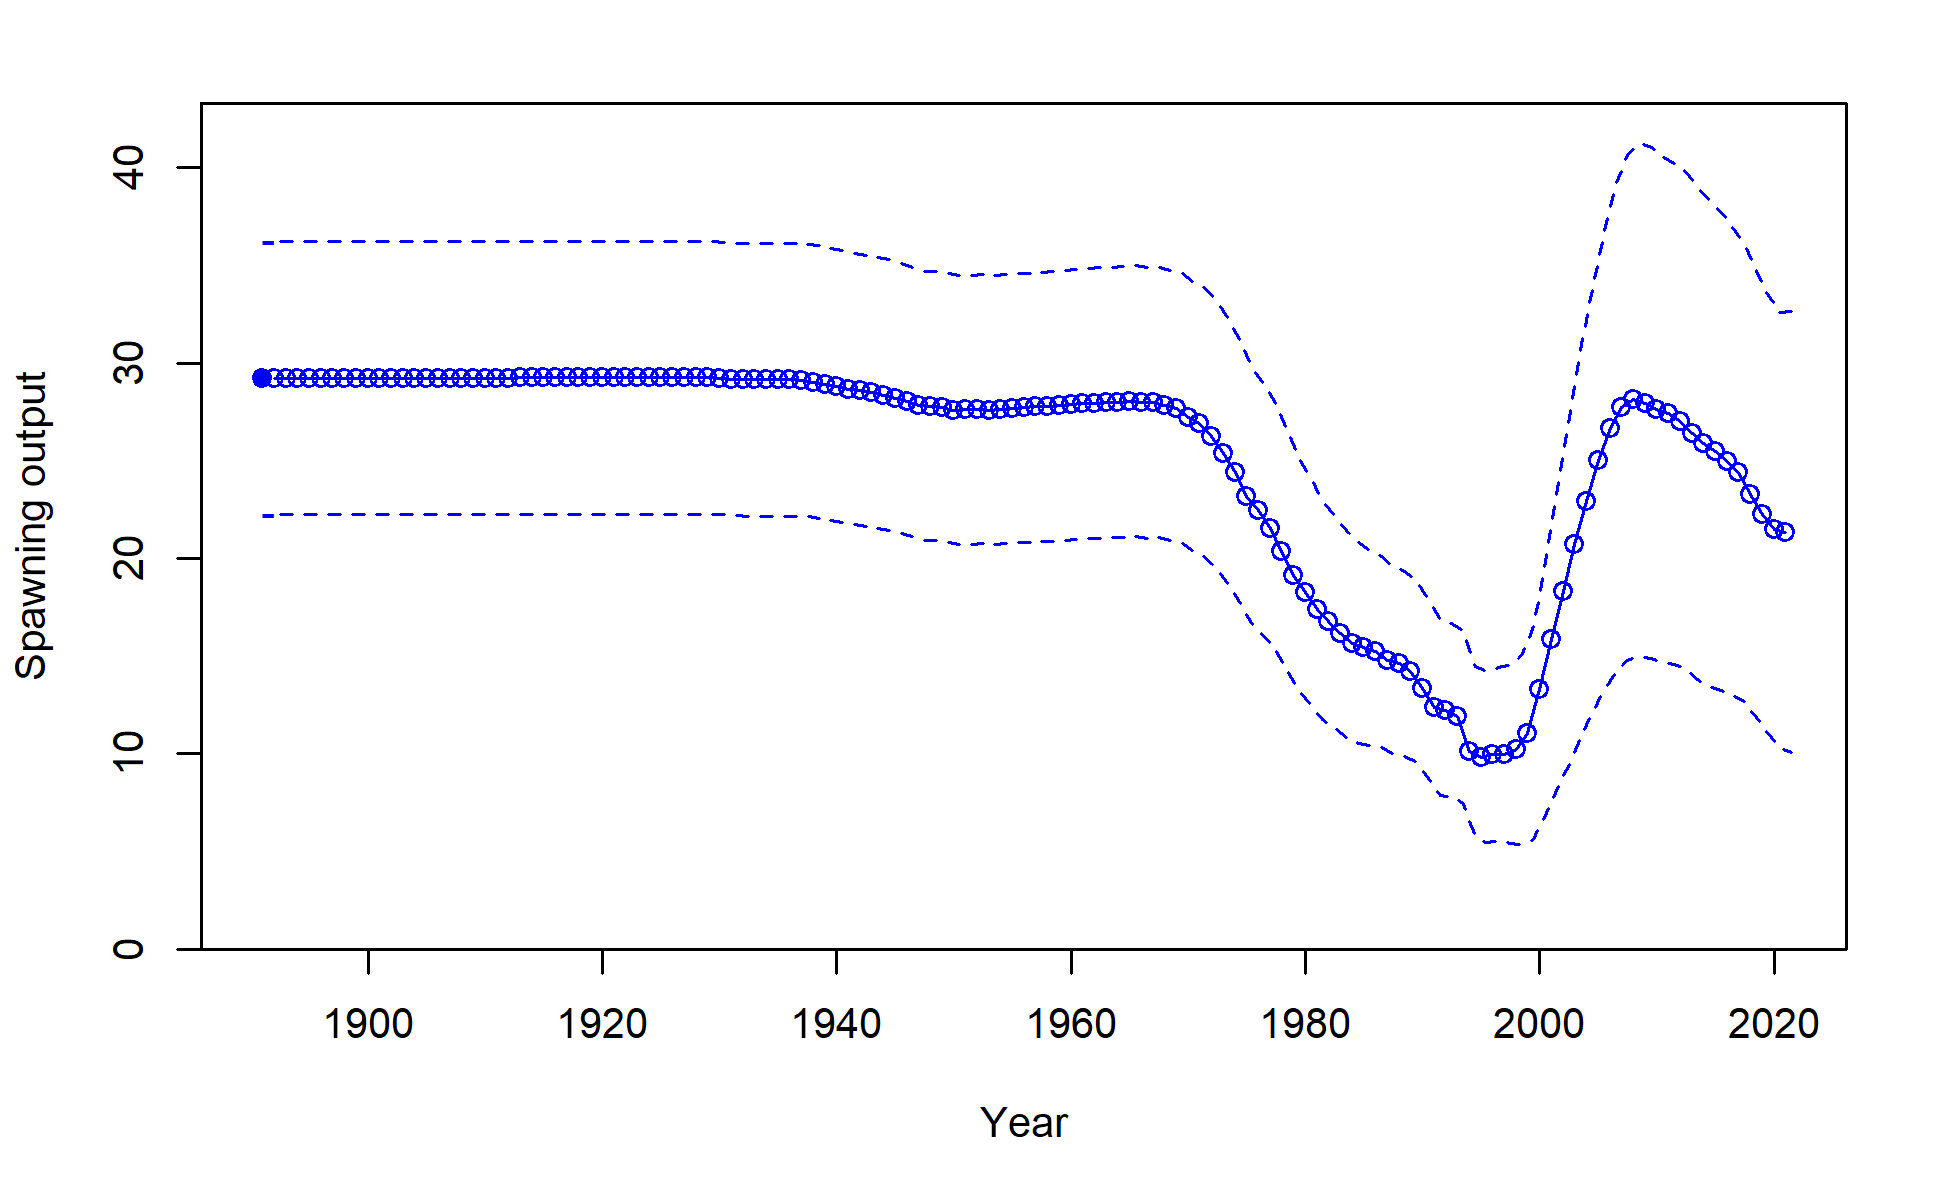
\includegraphics[width=1\textwidth,height=1\textheight]{C:/Users/Jason.Cope/Documents/Github/Vermilion rockfish OR WA assessment 2021/OR/write_up/models/Reference model/plots/ts7_Spawning_output_with_95_asymptotic_intervals_intervals.png}
\caption{Estimated time series of spawning biomass.\label{fig:ssb}}
\end{figure}

\tagmcend\tagstructend

\tagstructbegin{tag=Figure,alttext={Estimated time series of total biomass.}}\tagmcbegin{tag=Figure}

\begin{figure}
\centering
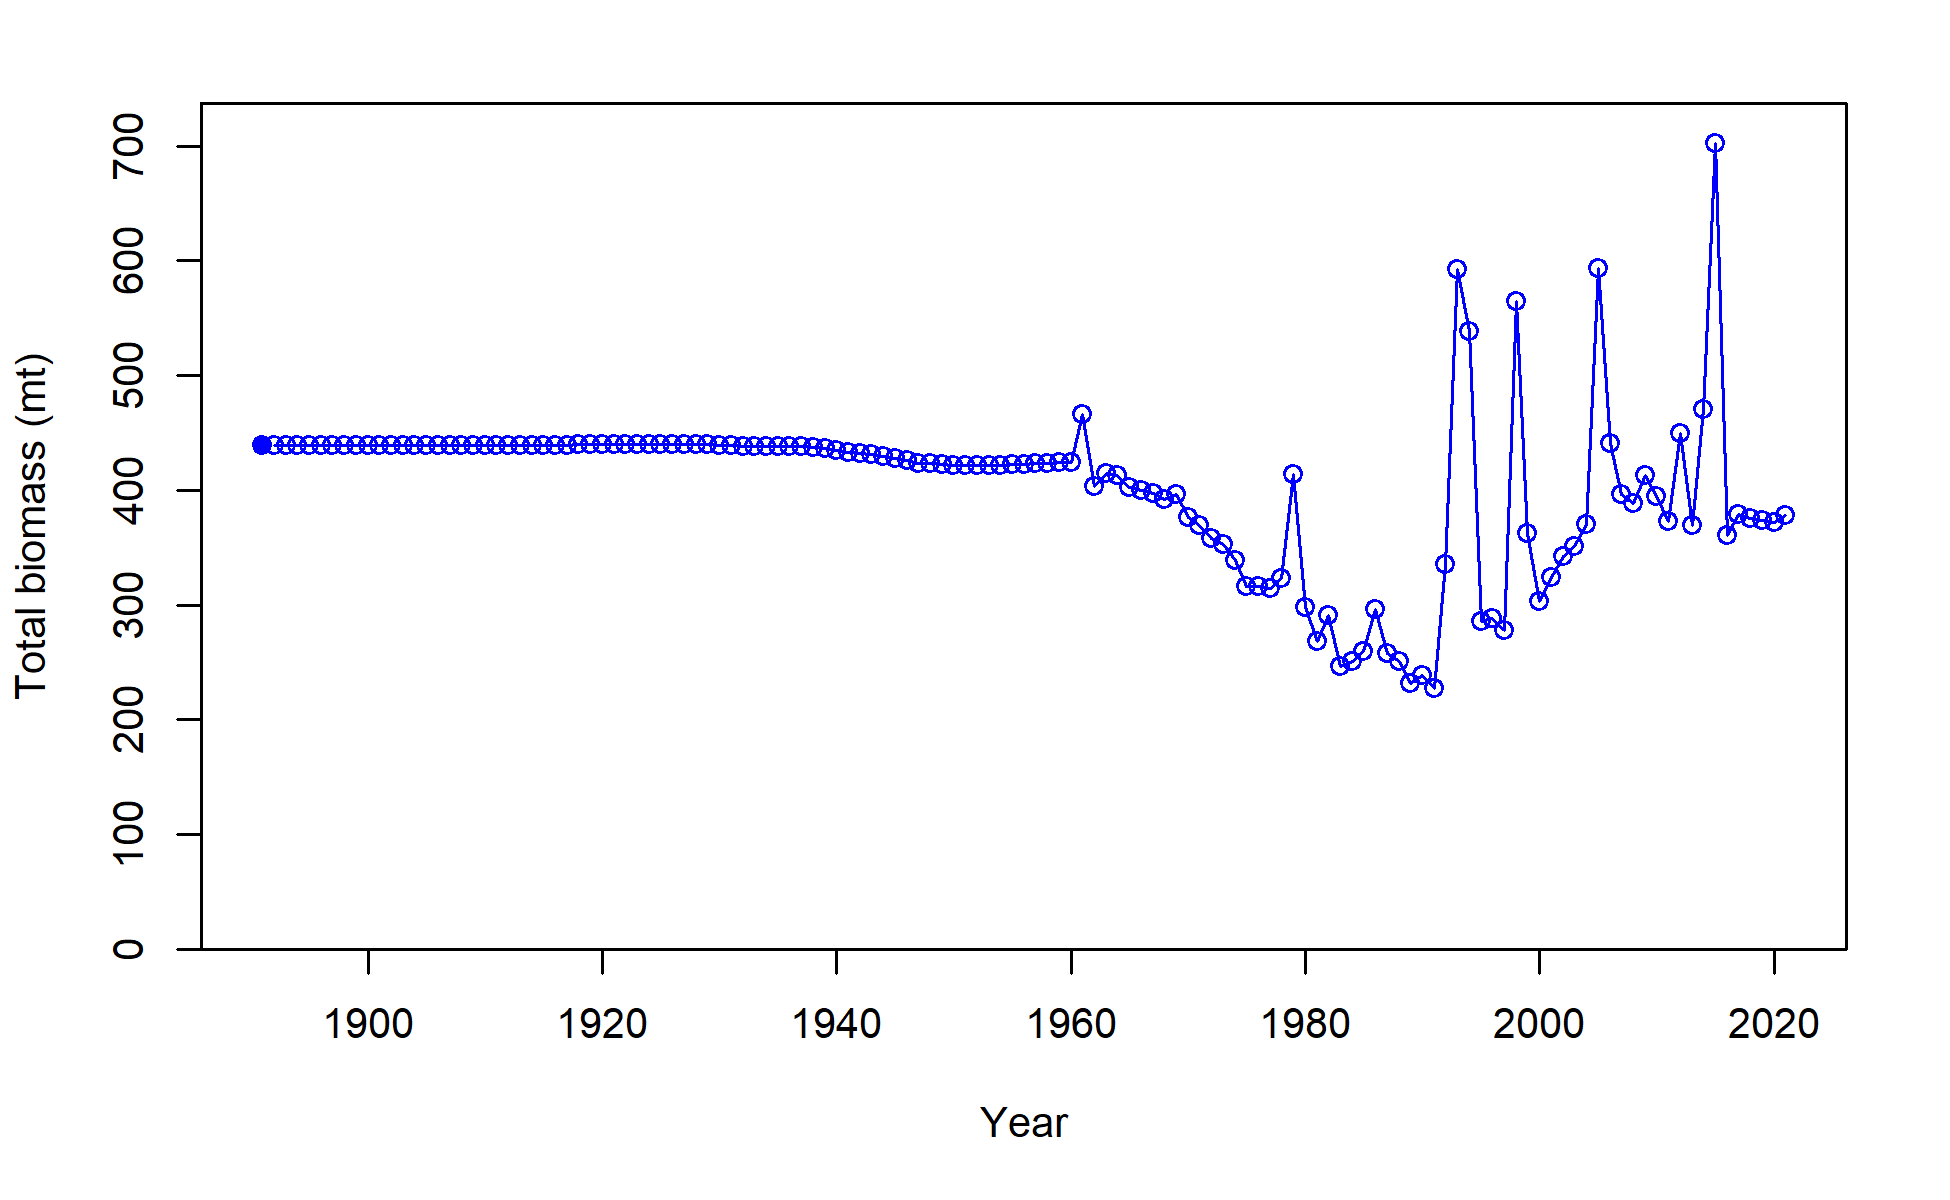
\includegraphics[width=1\textwidth,height=1\textheight]{C:/Users/Jason.Cope/Documents/Github/Vermilion rockfish OR WA assessment 2021/OR/write_up/models/Reference model/plots/ts1_Total_biomass_(mt).png}
\caption{Estimated time series of total biomass.\label{fig:tot-bio}}
\end{figure}

\tagmcend\tagstructend

\tagstructbegin{tag=Figure,alttext={Estimated time series of fraction of unfished spawning biomass.}}\tagmcbegin{tag=Figure}

\begin{figure}
\centering
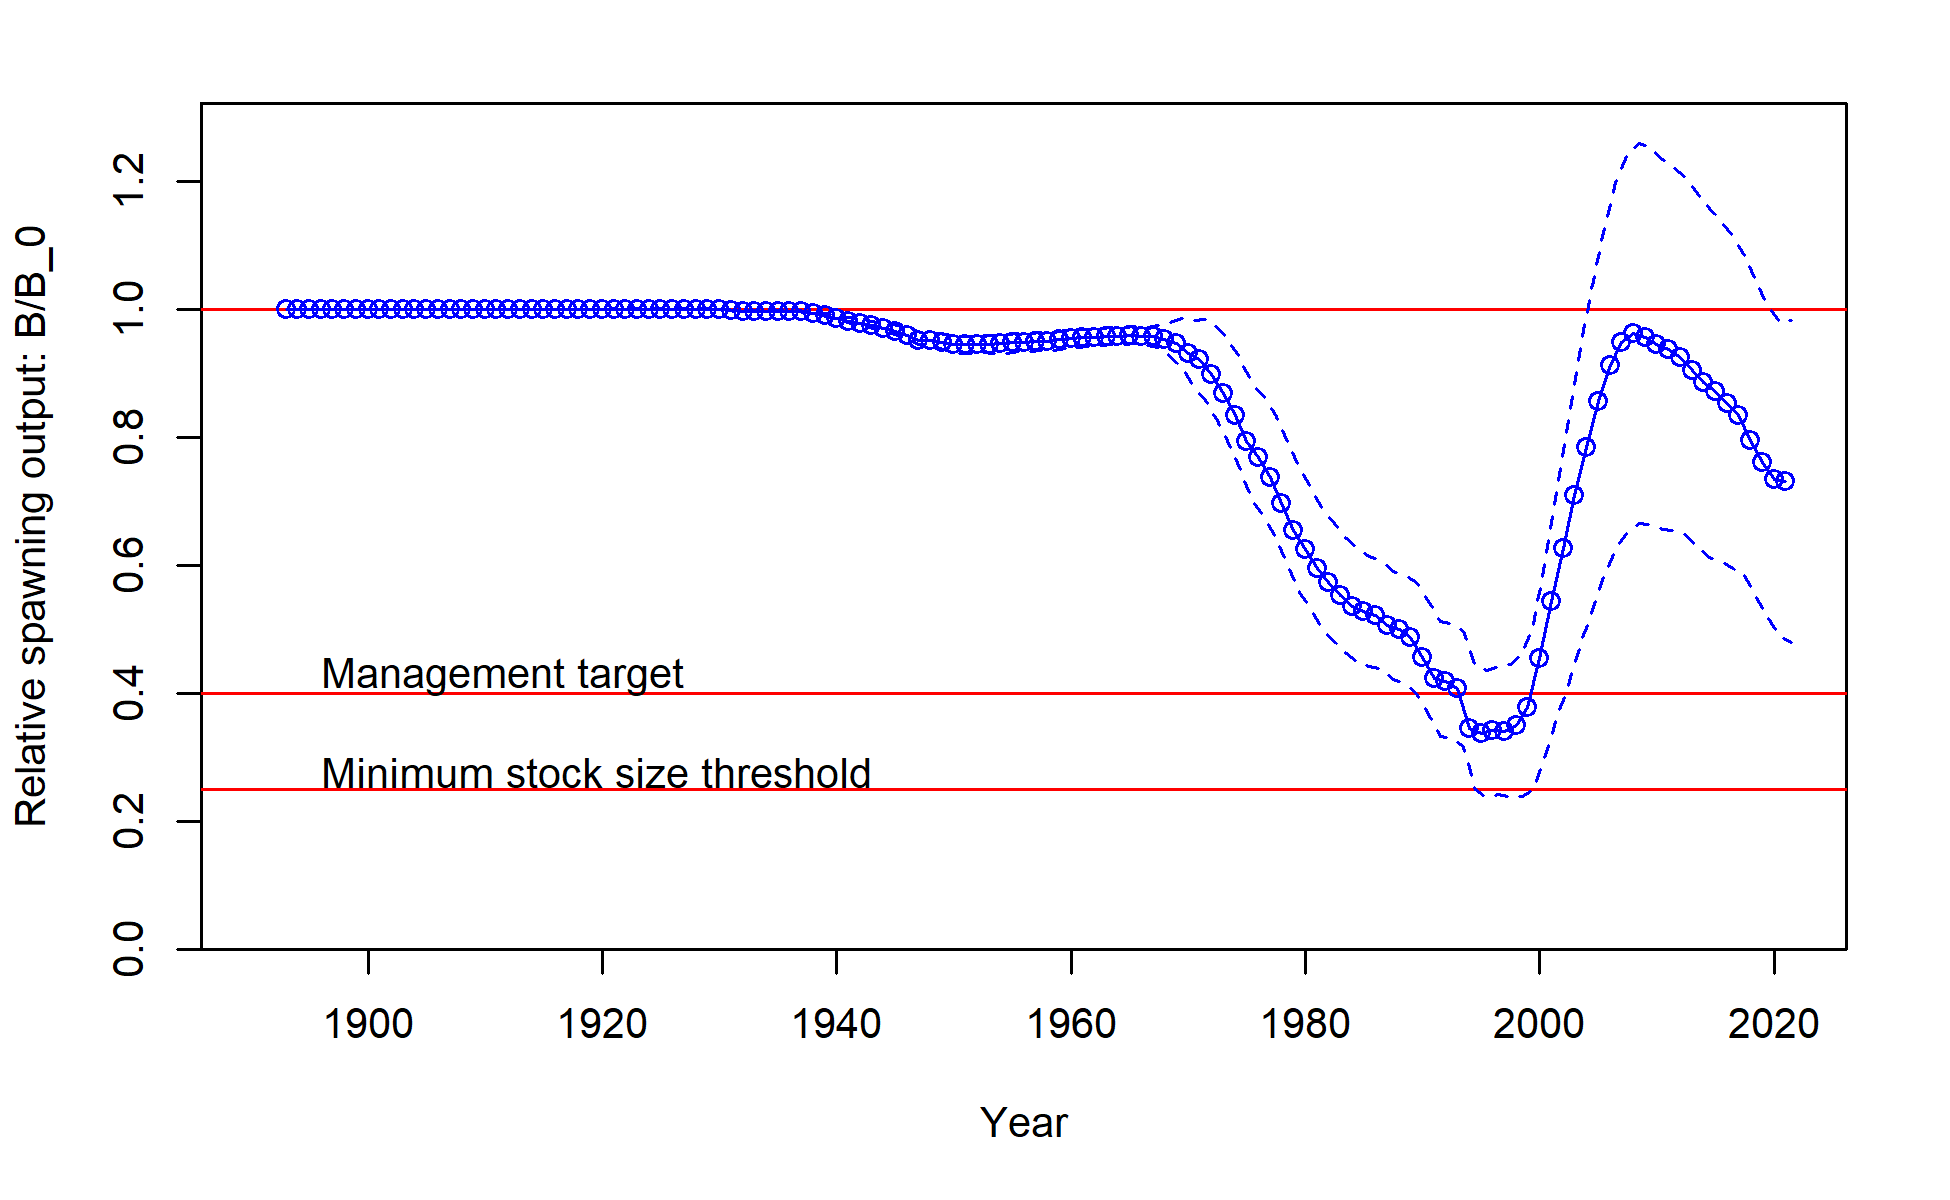
\includegraphics[width=1\textwidth,height=1\textheight]{C:/Users/Jason.Cope/Documents/Github/Vermilion rockfish OR WA assessment 2021/OR/write_up/models/Reference model/plots/ts9_Relative_spawning_output_intervals.png}
\caption{Estimated time series of fraction of unfished spawning biomass.\label{fig:depl}}
\end{figure}

\tagmcend\tagstructend

\tagstructbegin{tag=Figure,alttext={Estimated time series of age-0 recruits (1000s).}}\tagmcbegin{tag=Figure}

\begin{figure}
\centering
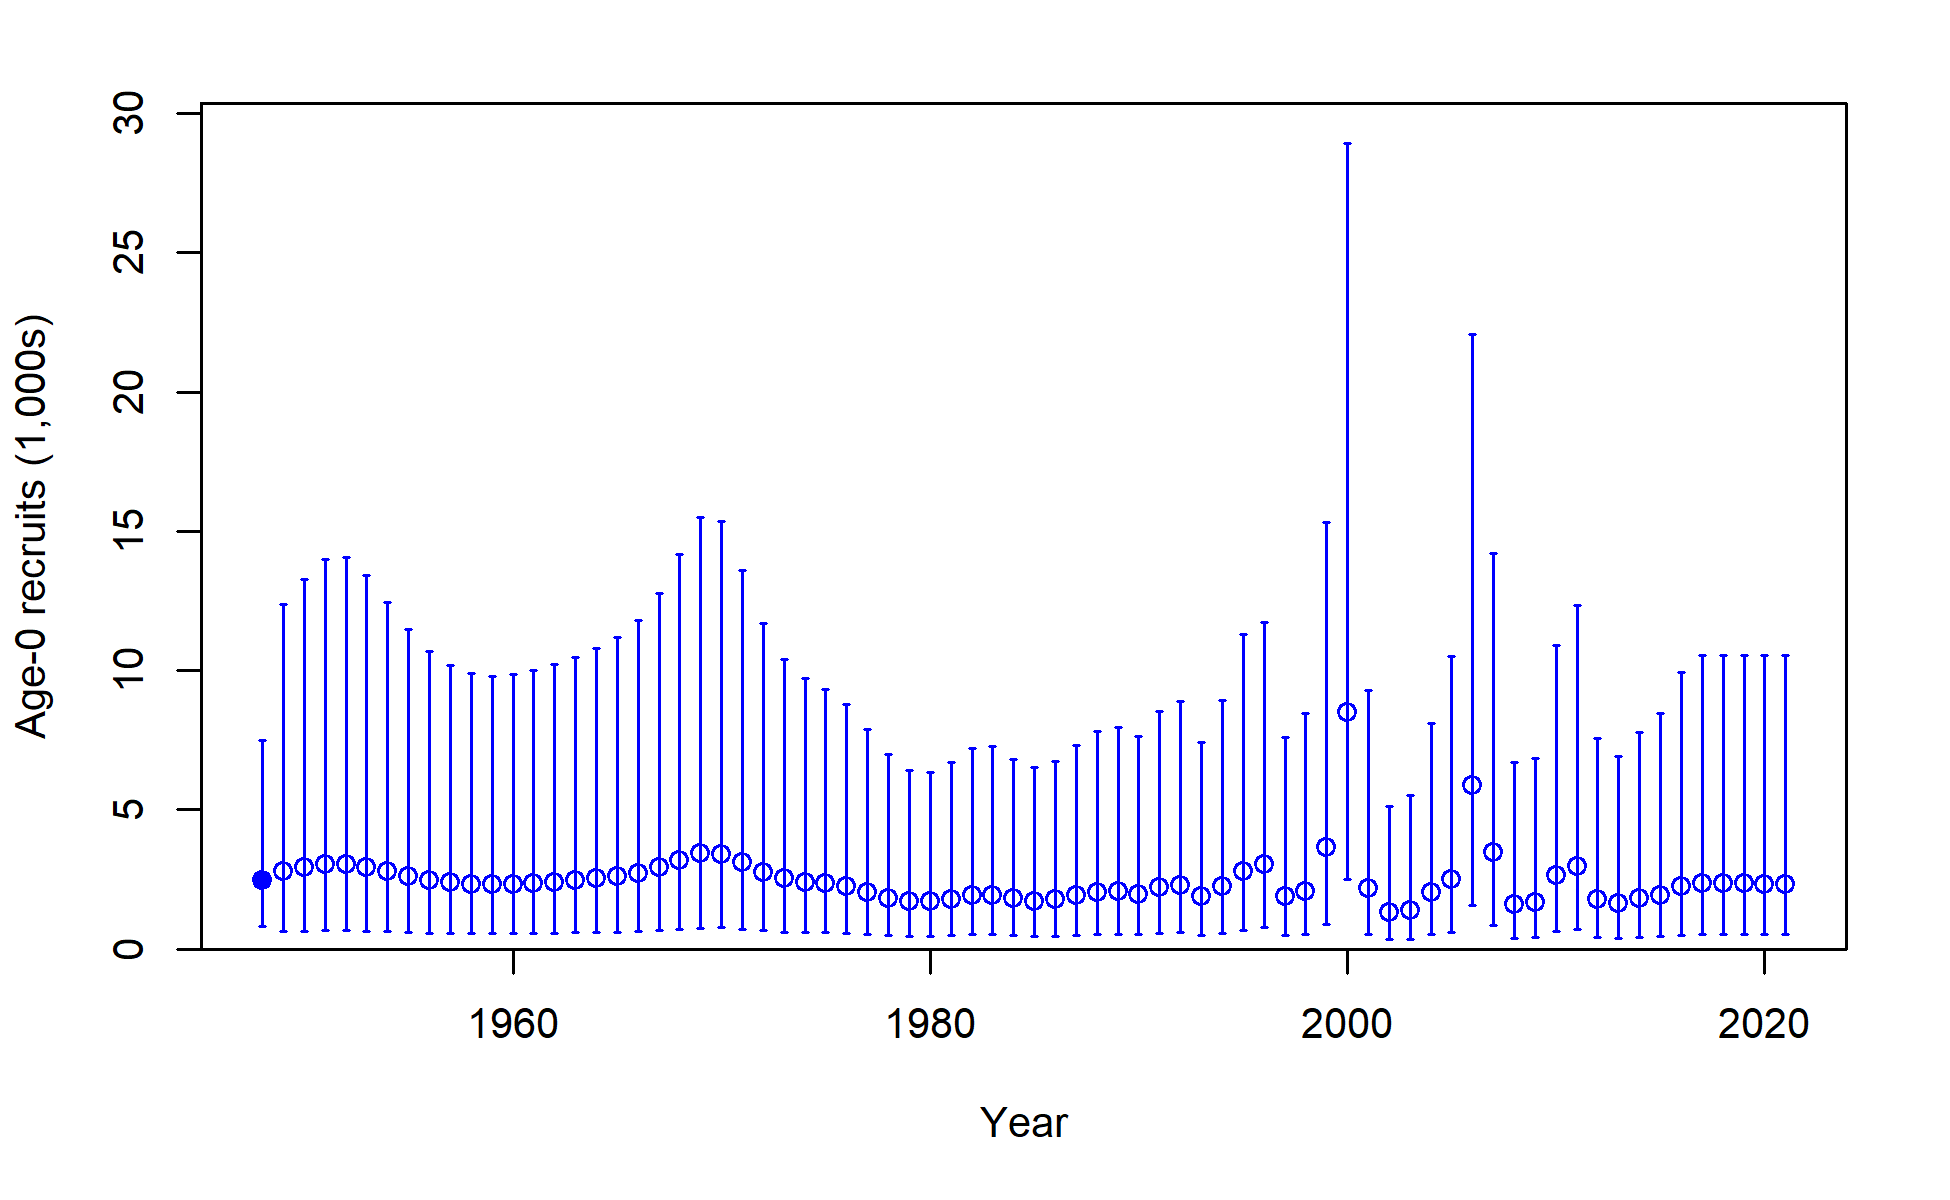
\includegraphics[width=1\textwidth,height=1\textheight]{C:/Users/Jason.Cope/Documents/Github/Vermilion rockfish OR WA assessment 2021/OR/write_up/models/Reference model/plots/ts11_Age-0_recruits_(1000s)_with_95_asymptotic_intervals.png}
\caption{Estimated time series of age-0 recruits (1000s).\label{fig:recruits}}
\end{figure}

\tagmcend\tagstructend

\tagstructbegin{tag=Figure,alttext={Estimated time series of recruitment deviations.}}\tagmcbegin{tag=Figure}

\begin{figure}
\centering
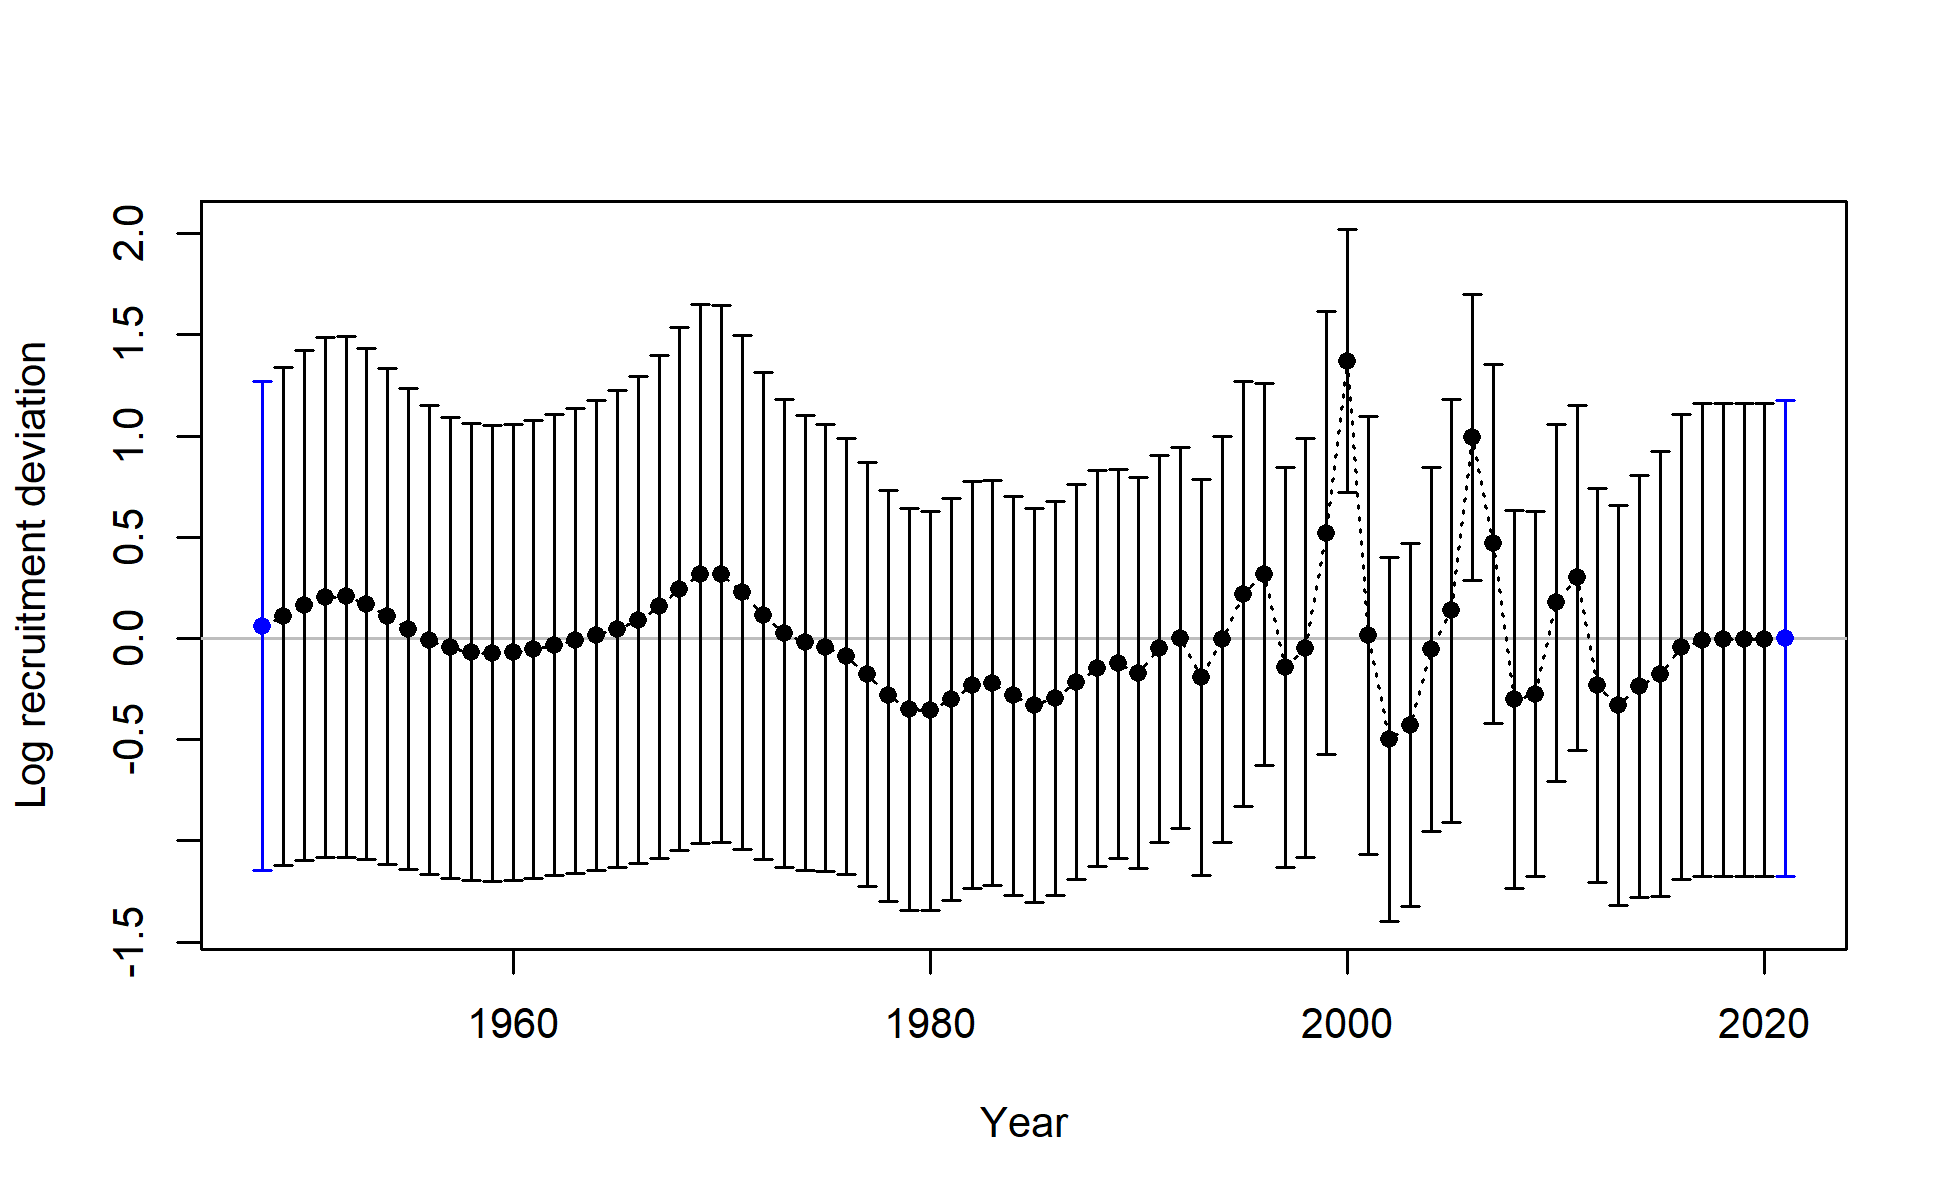
\includegraphics[width=1\textwidth,height=1\textheight]{C:/Users/Jason.Cope/Documents/Github/Vermilion rockfish OR WA assessment 2021/OR/write_up/models/Reference model/plots/recdevs2_withbars.png}
\caption{Estimated time series of recruitment deviations.\label{fig:rec-devs}}
\end{figure}

\tagmcend\tagstructend

\tagstructbegin{tag=Figure,alttext={Recruitment deviations variance by year. This plot tracks the information content contained in each recruitment deviation. Values below the red line (assumed recruitment variability) indicates years with more informed recruitment deviations.}}\tagmcbegin{tag=Figure}

\begin{figure}
\centering
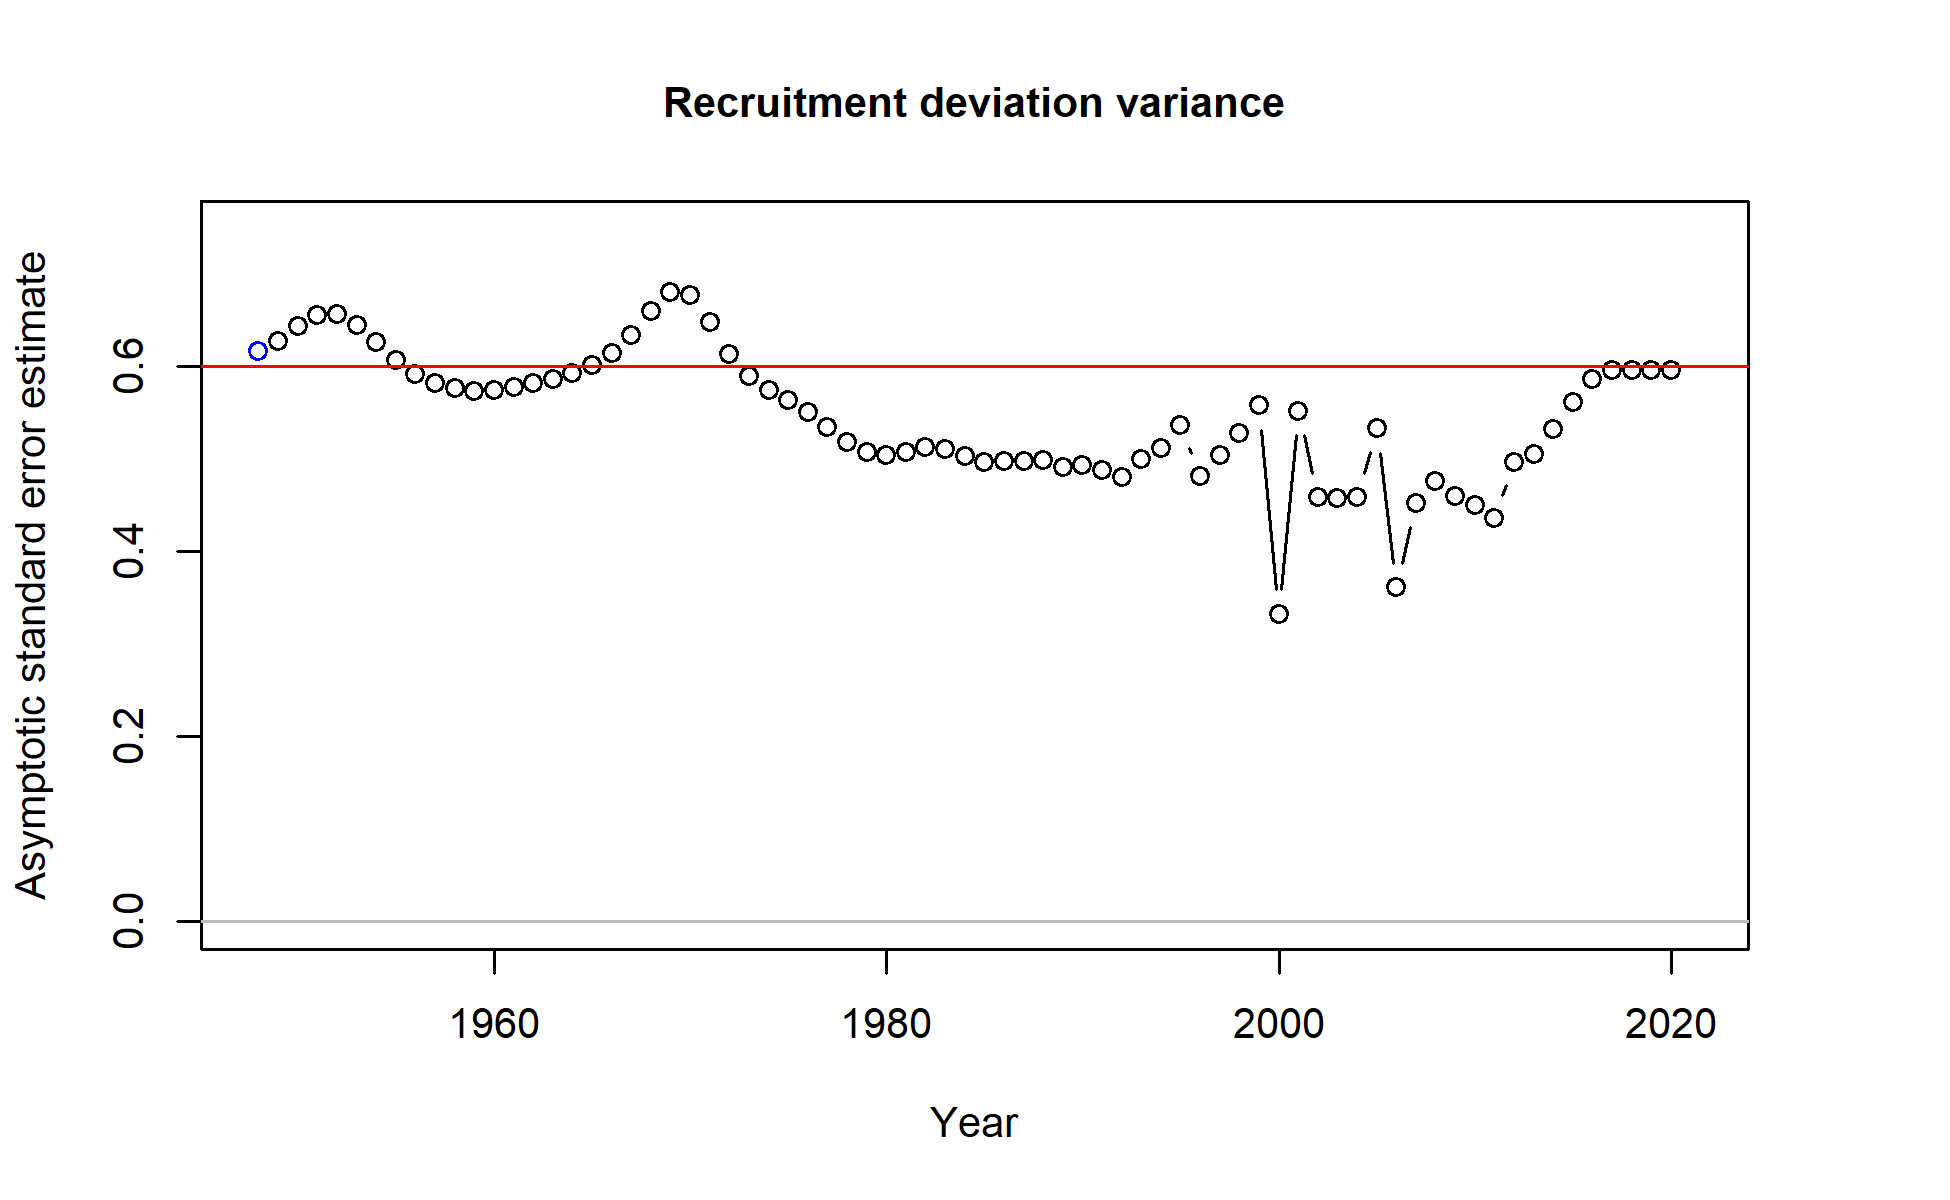
\includegraphics[width=1\textwidth,height=1\textheight]{C:/Users/Jason.Cope/Documents/Github/Vermilion rockfish OR WA assessment 2021/OR/write_up/models/Reference model/plots/recdevs3_varcheck.png}
\caption{Recruitment deviations variance by year. This plot tracks the information content contained in each recruitment deviation. Values below the red line (assumed recruitment variability) indicates years with more informed recruitment deviations.\label{fig:rec-devs-sigmas}}
\end{figure}

\tagmcend\tagstructend

\tagstructbegin{tag=Figure,alttext={Stock-recruit curve. Point colors indicate year, with warmer colors indicating earlier years and cooler colors in showing later years.}}\tagmcbegin{tag=Figure}

\begin{figure}
\centering
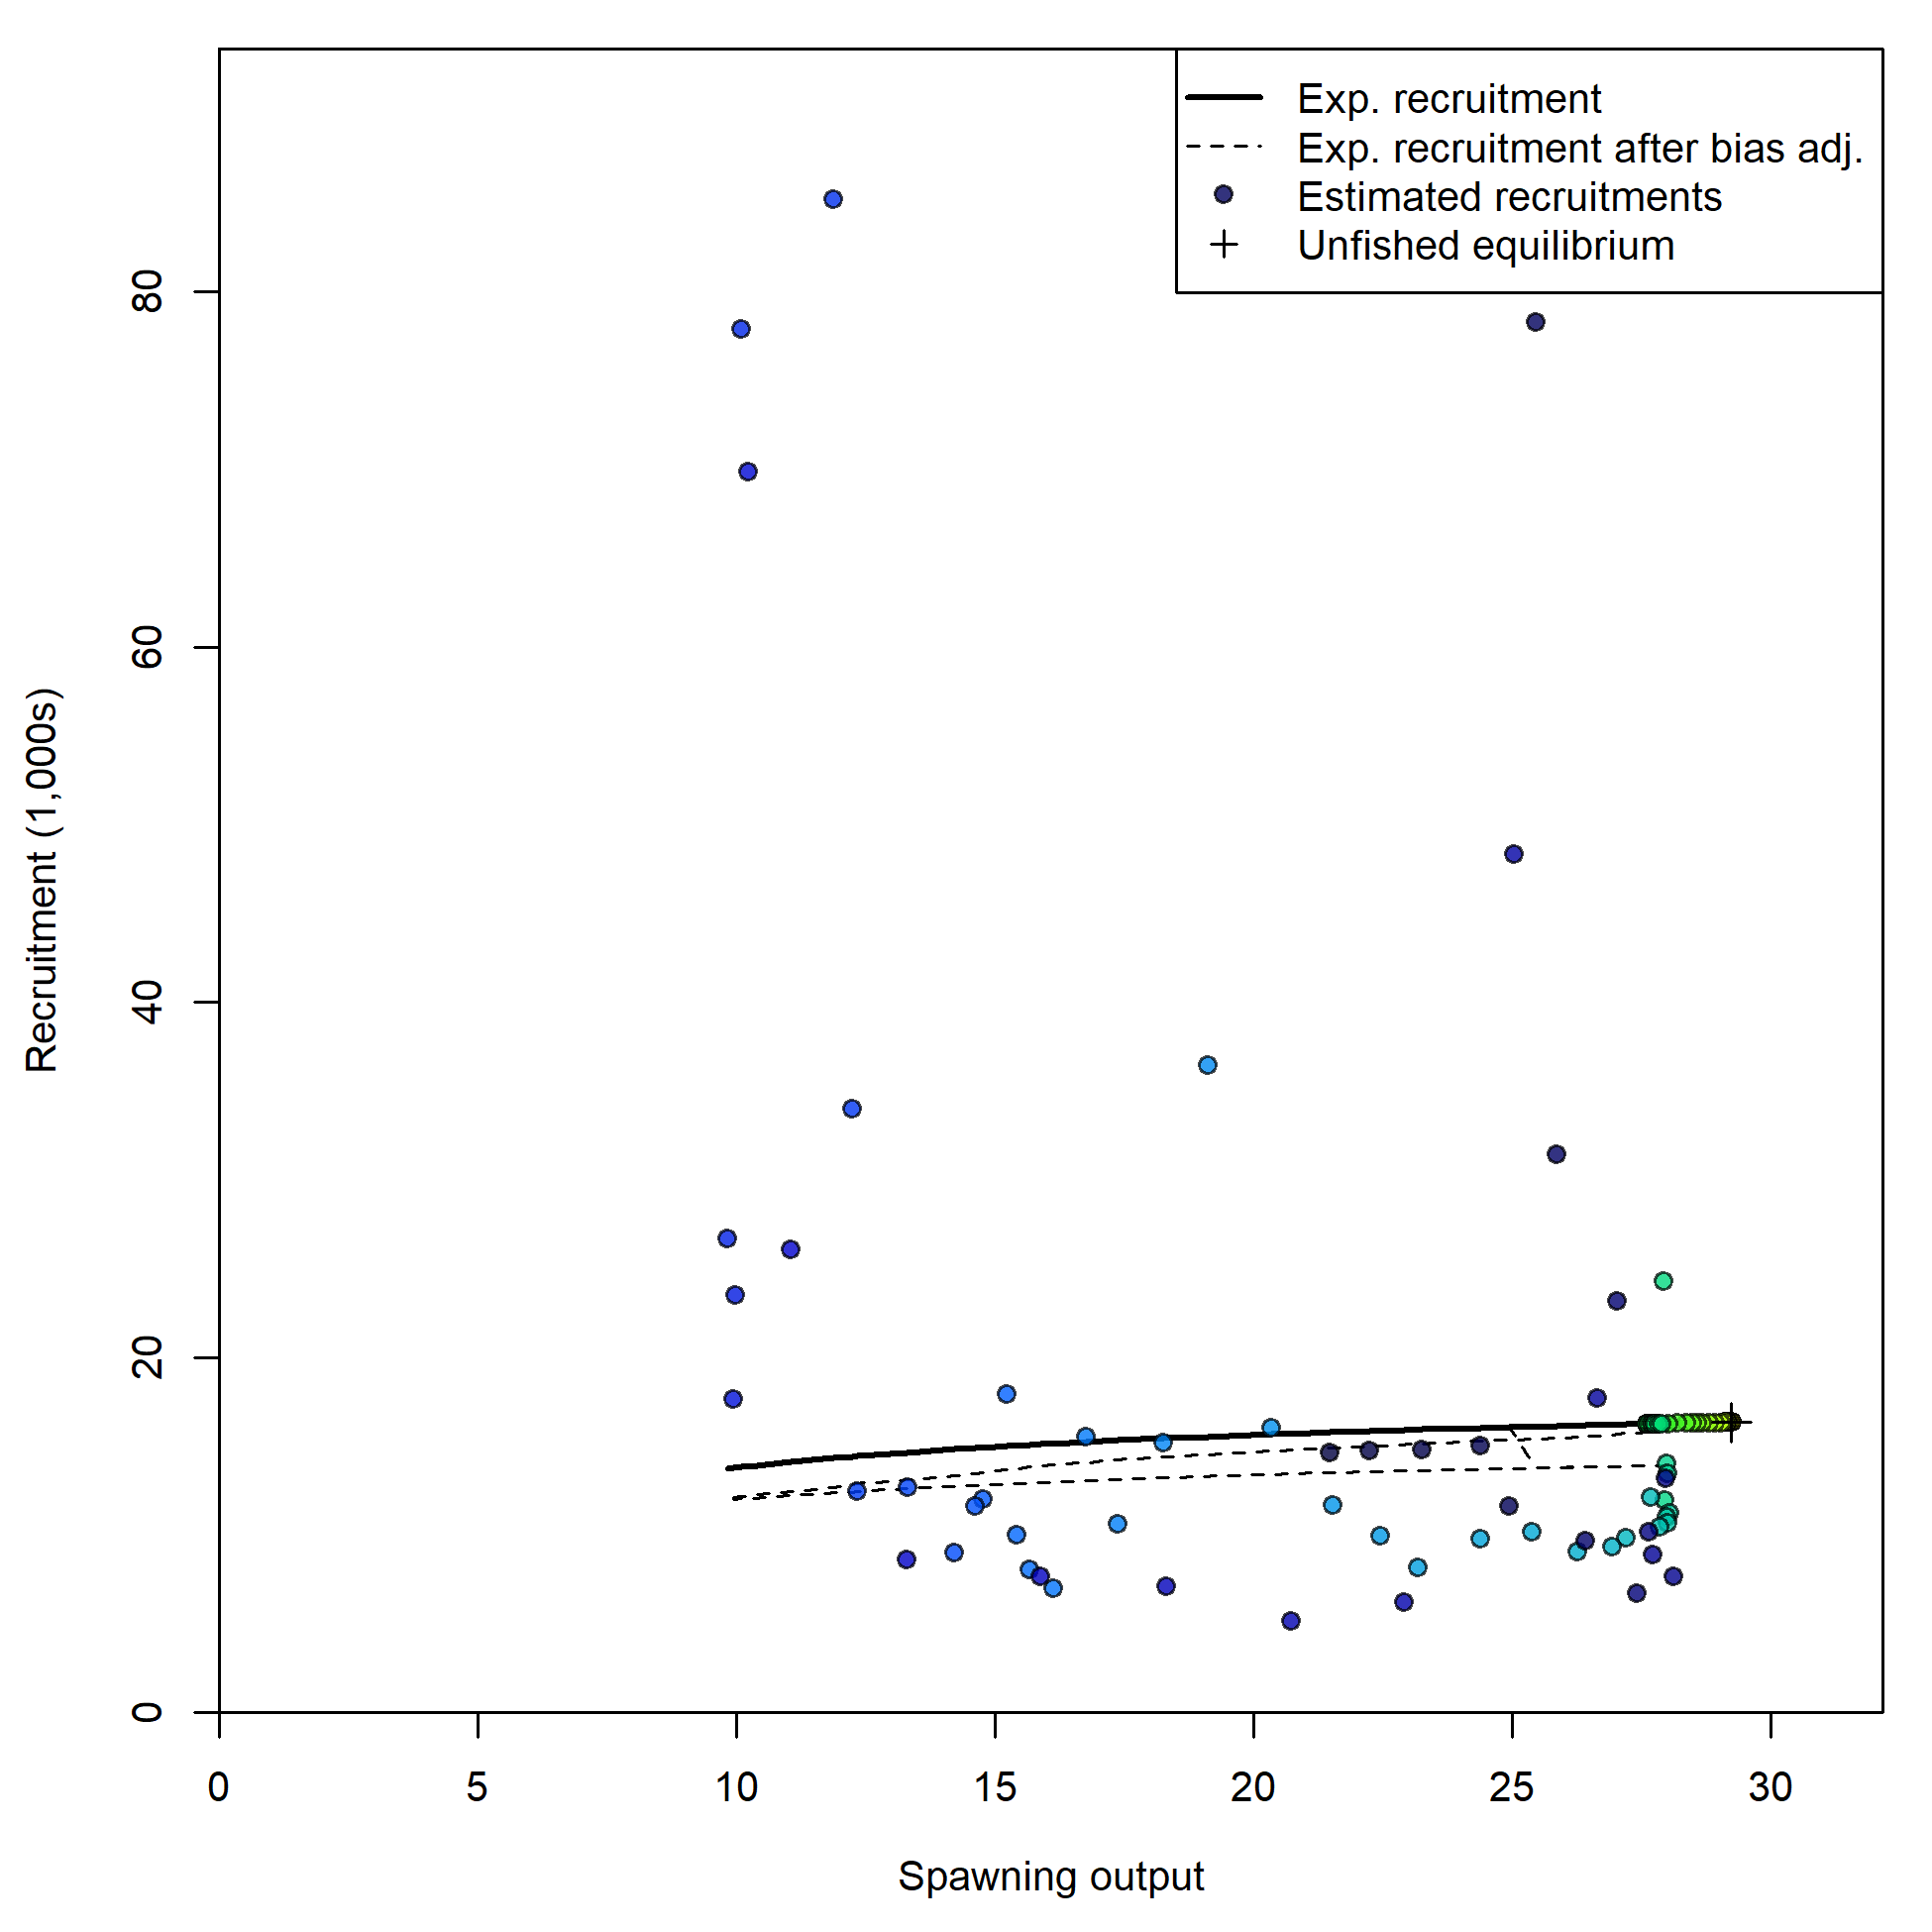
\includegraphics[width=1\textwidth,height=1\textheight]{C:/Users/Jason.Cope/Documents/Github/Vermilion rockfish OR WA assessment 2021/OR/write_up/models/Reference model/plots/SR_curve.png}
\caption{Stock-recruit curve. Point colors indicate year, with warmer colors indicating earlier years and cooler colors in showing later years.\label{fig:bh-curve}}
\end{figure}

\tagmcend\tagstructend

\tagstructbegin{tag=Figure,alttext={Recruitment bias adjustment applied in the base model.}}\tagmcbegin{tag=Figure}

\begin{figure}
\centering
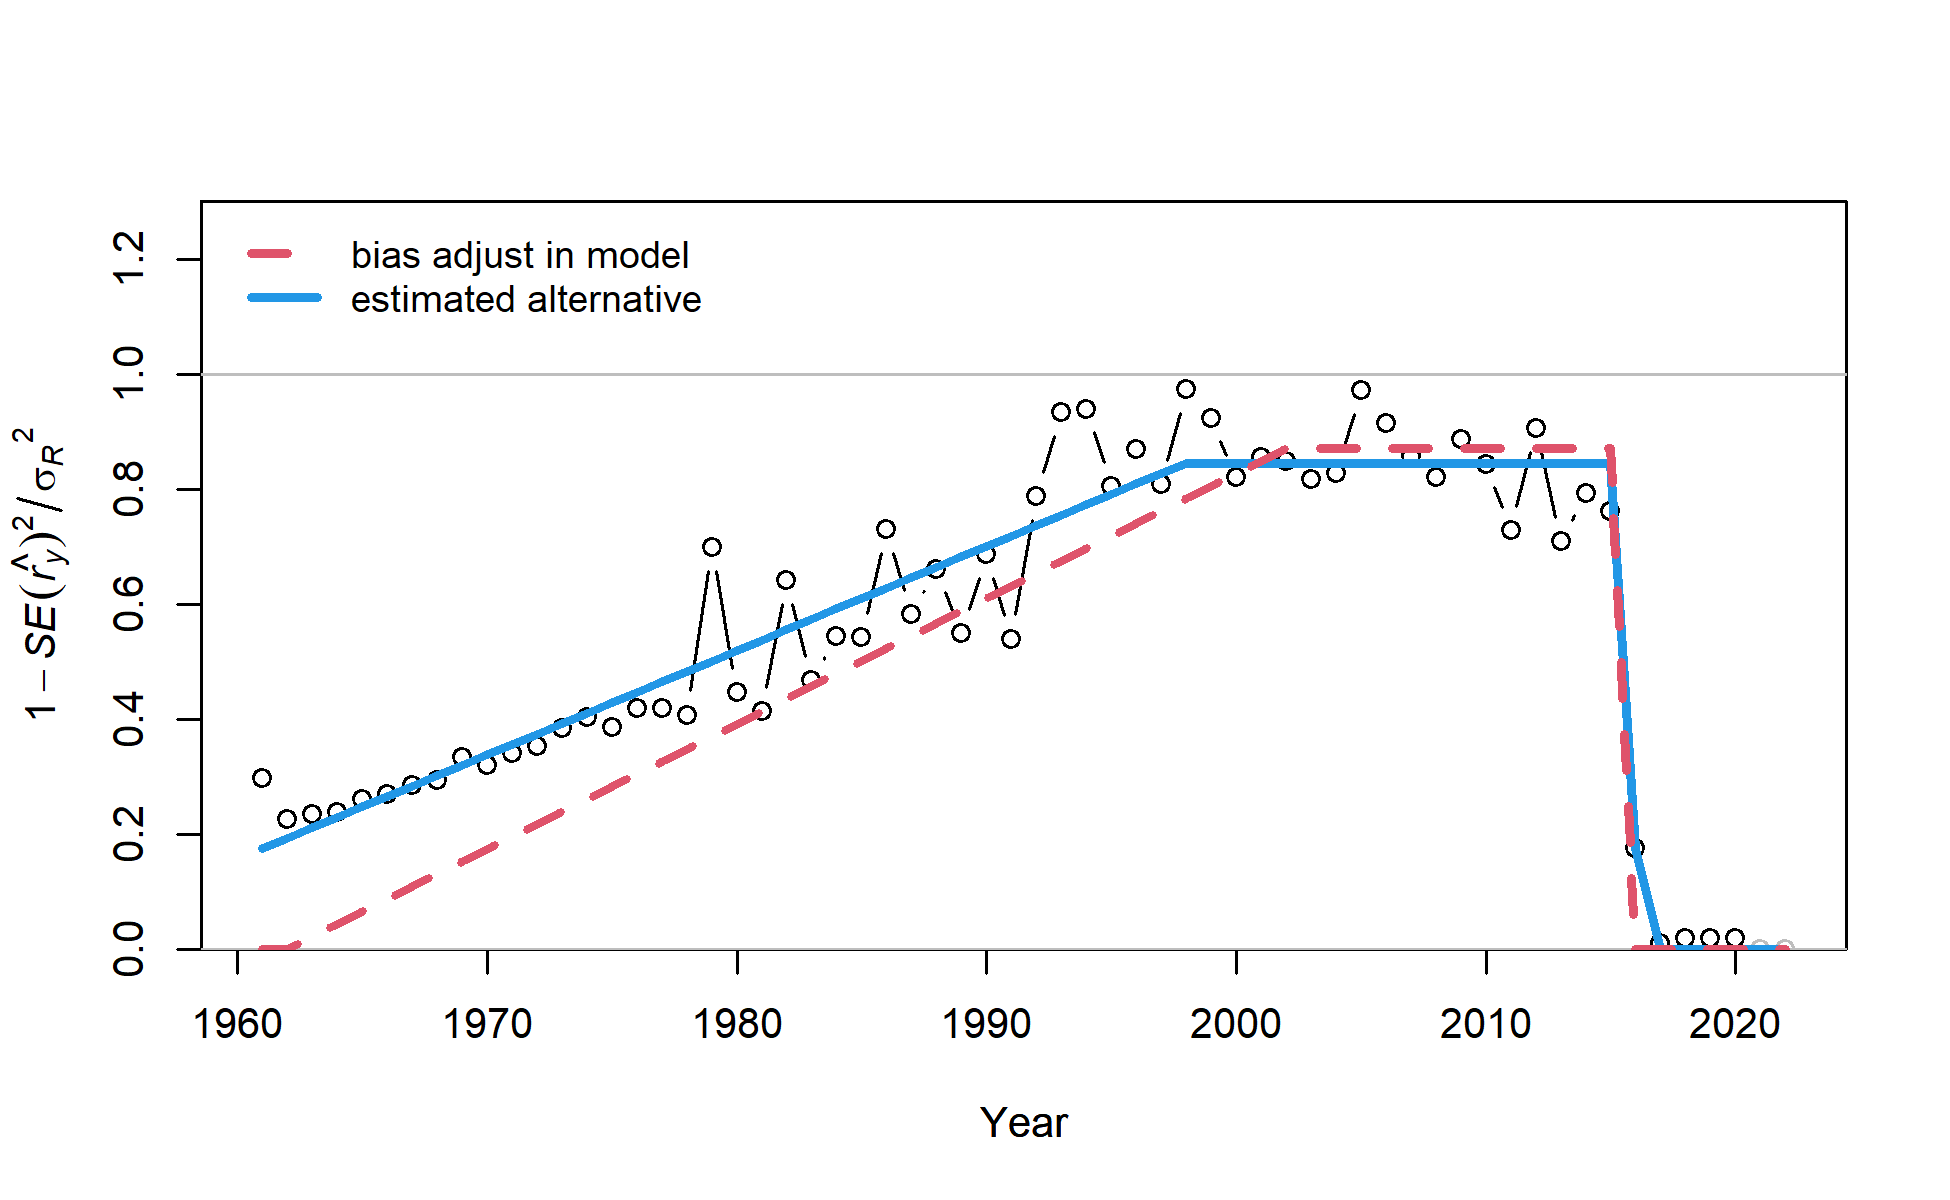
\includegraphics[width=1\textwidth,height=1\textheight]{C:/Users/Jason.Cope/Documents/Github/Vermilion rockfish OR WA assessment 2021/OR/write_up/models/Reference model/plots/recruit_fit_bias_adjust.png}
\caption{Recruitment bias adjustment applied in the base model.\label{fig:bias-adj}}
\end{figure}

\tagmcend\tagstructend

\tagstructbegin{tag=Figure,alttext={Stock recruit curve where point color indicate year, with warmer colors (yellow to green) indicating earlier years and cooler colors (blue) showing later years.}}\tagmcbegin{tag=Figure}

\begin{figure}
\centering
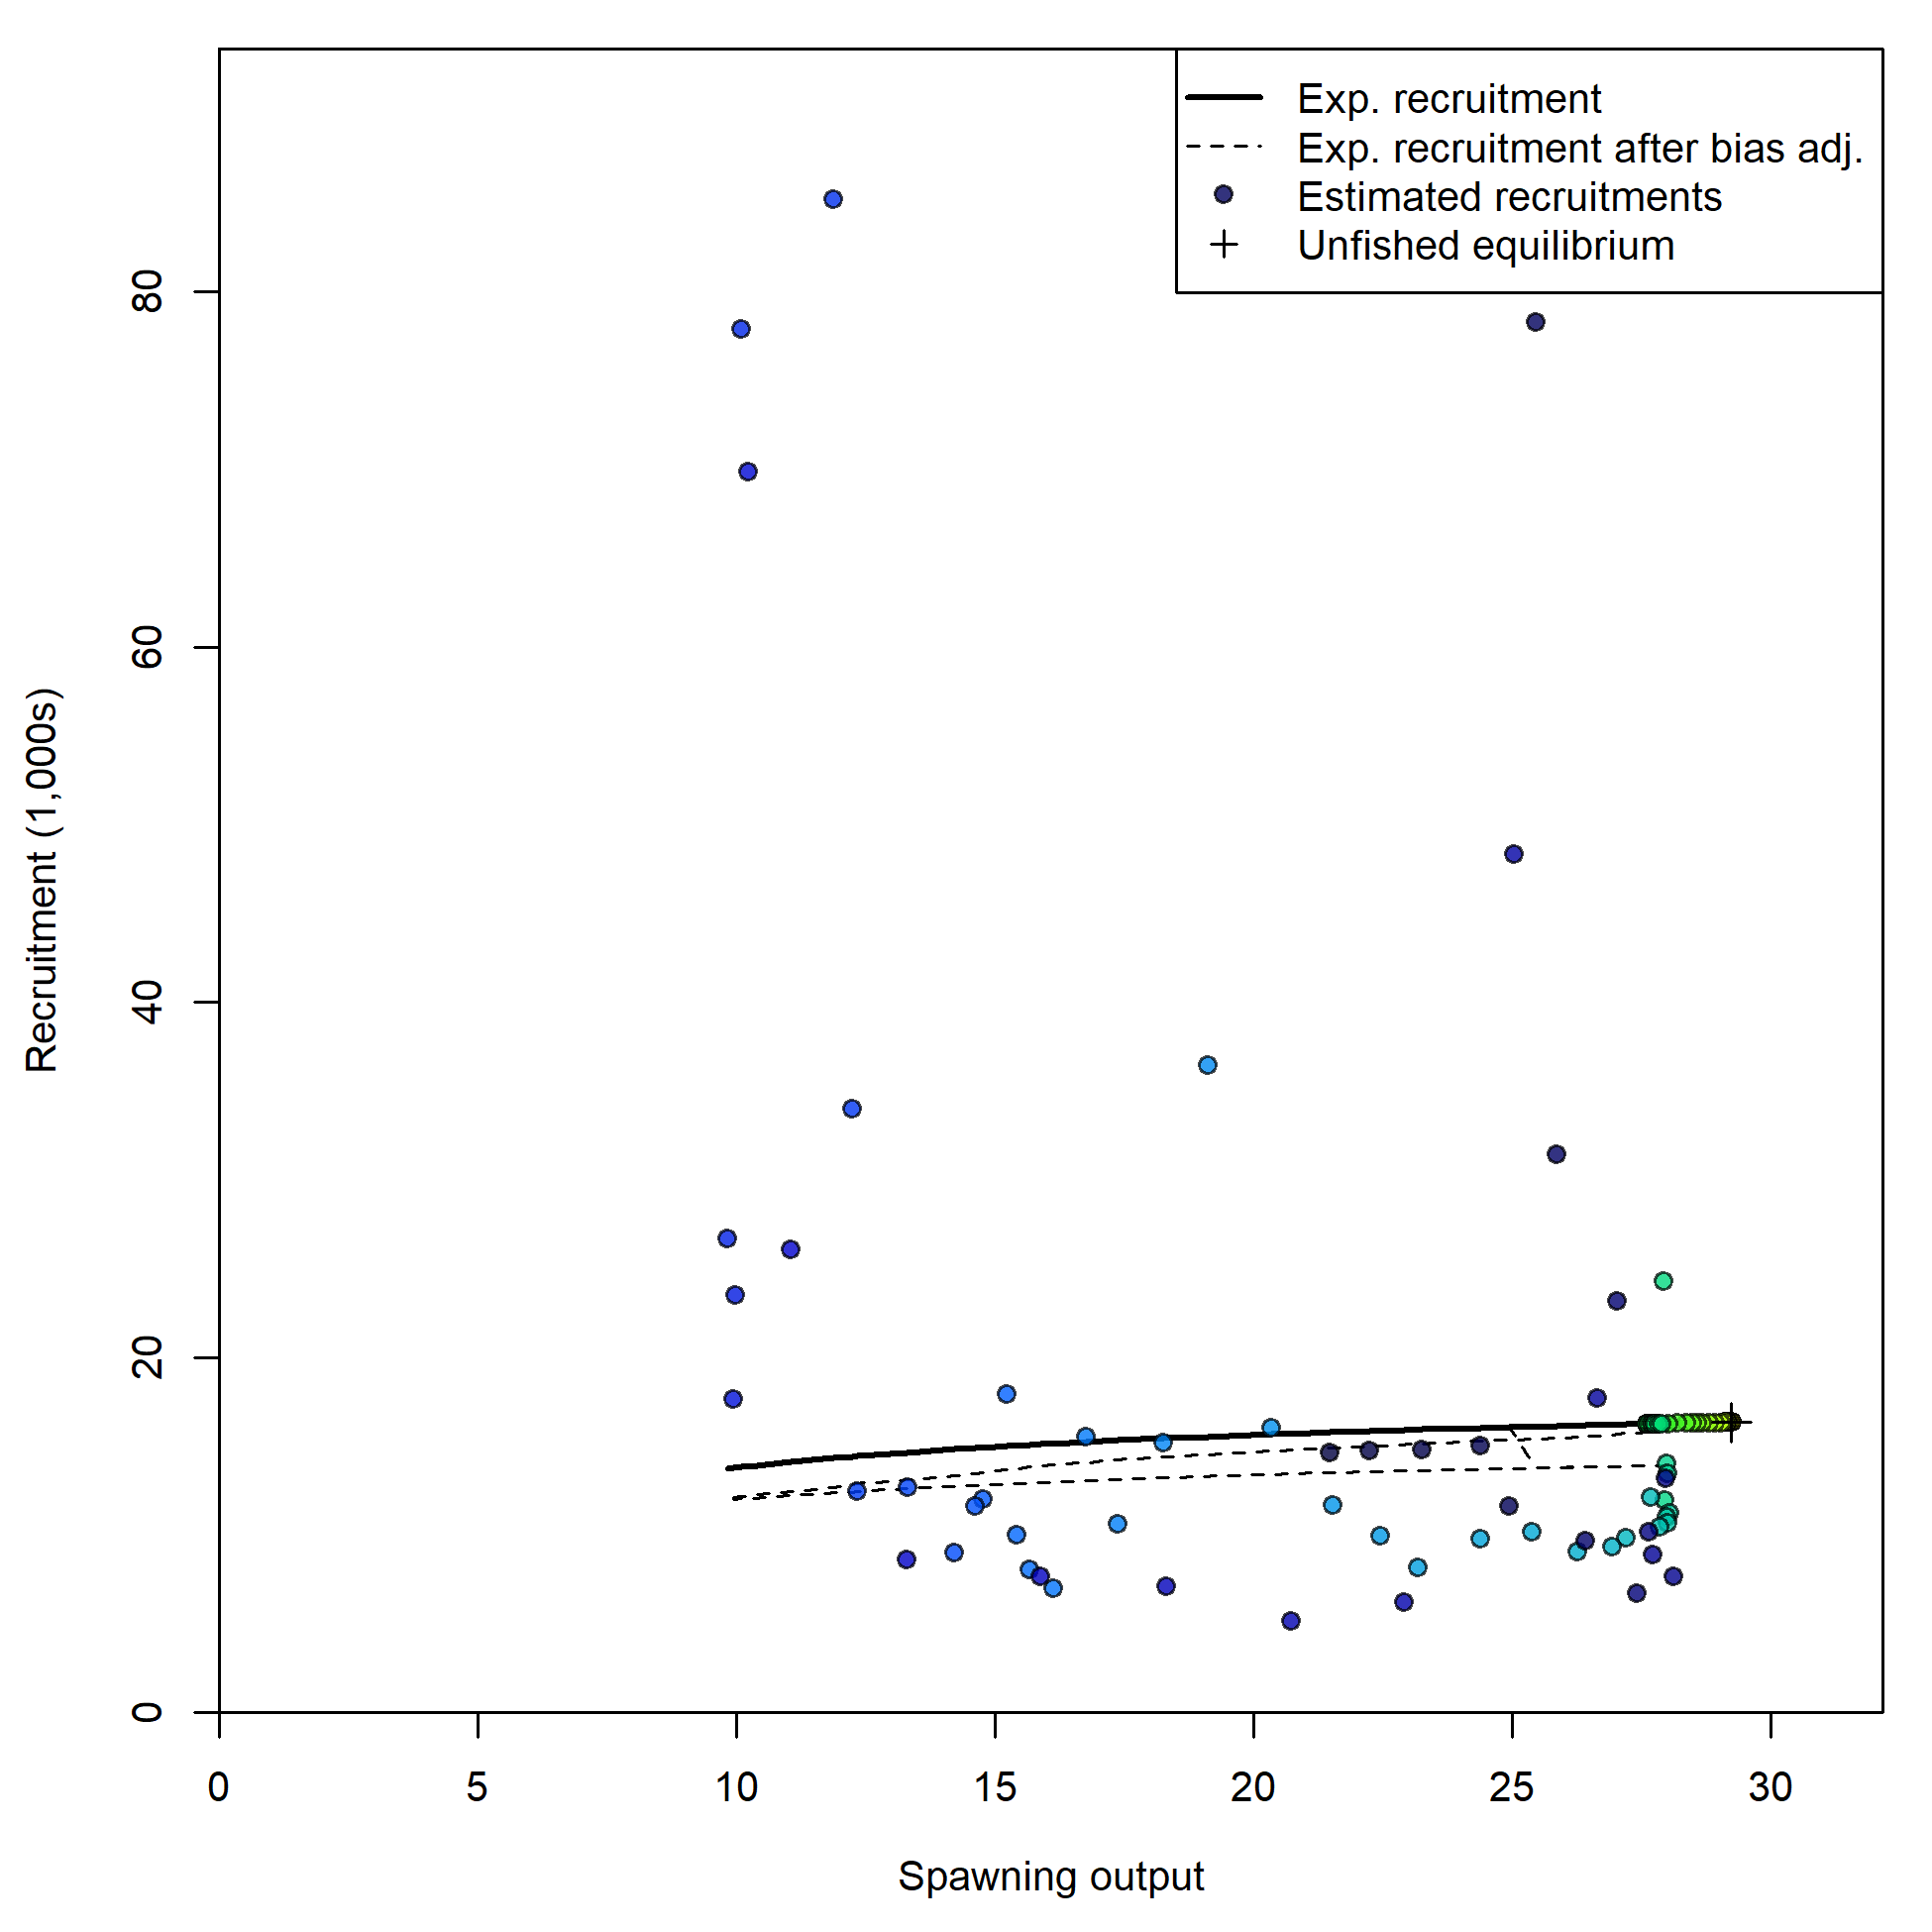
\includegraphics[width=1\textwidth,height=1\textheight]{C:/Users/Jason.Cope/Documents/Github/Vermilion rockfish OR WA assessment 2021/OR/write_up/models/Reference model/plots/SR_curve.png}
\caption{Stock recruit curve where point color indicate year, with warmer colors (yellow to green) indicating earlier years and cooler colors (blue) showing later years.\label{fig:sr-curve}}
\end{figure}

\tagmcend\tagstructend

\tagstructbegin{tag=Figure,alttext={Log relative change (log((Model_sensi-Model_ref)/Model_ref)) in data treatment for 5 derived quantities. Colored boxes indicate 95 percent confidence interval of the reference model.}}\tagmcbegin{tag=Figure}

\begin{figure}
\centering
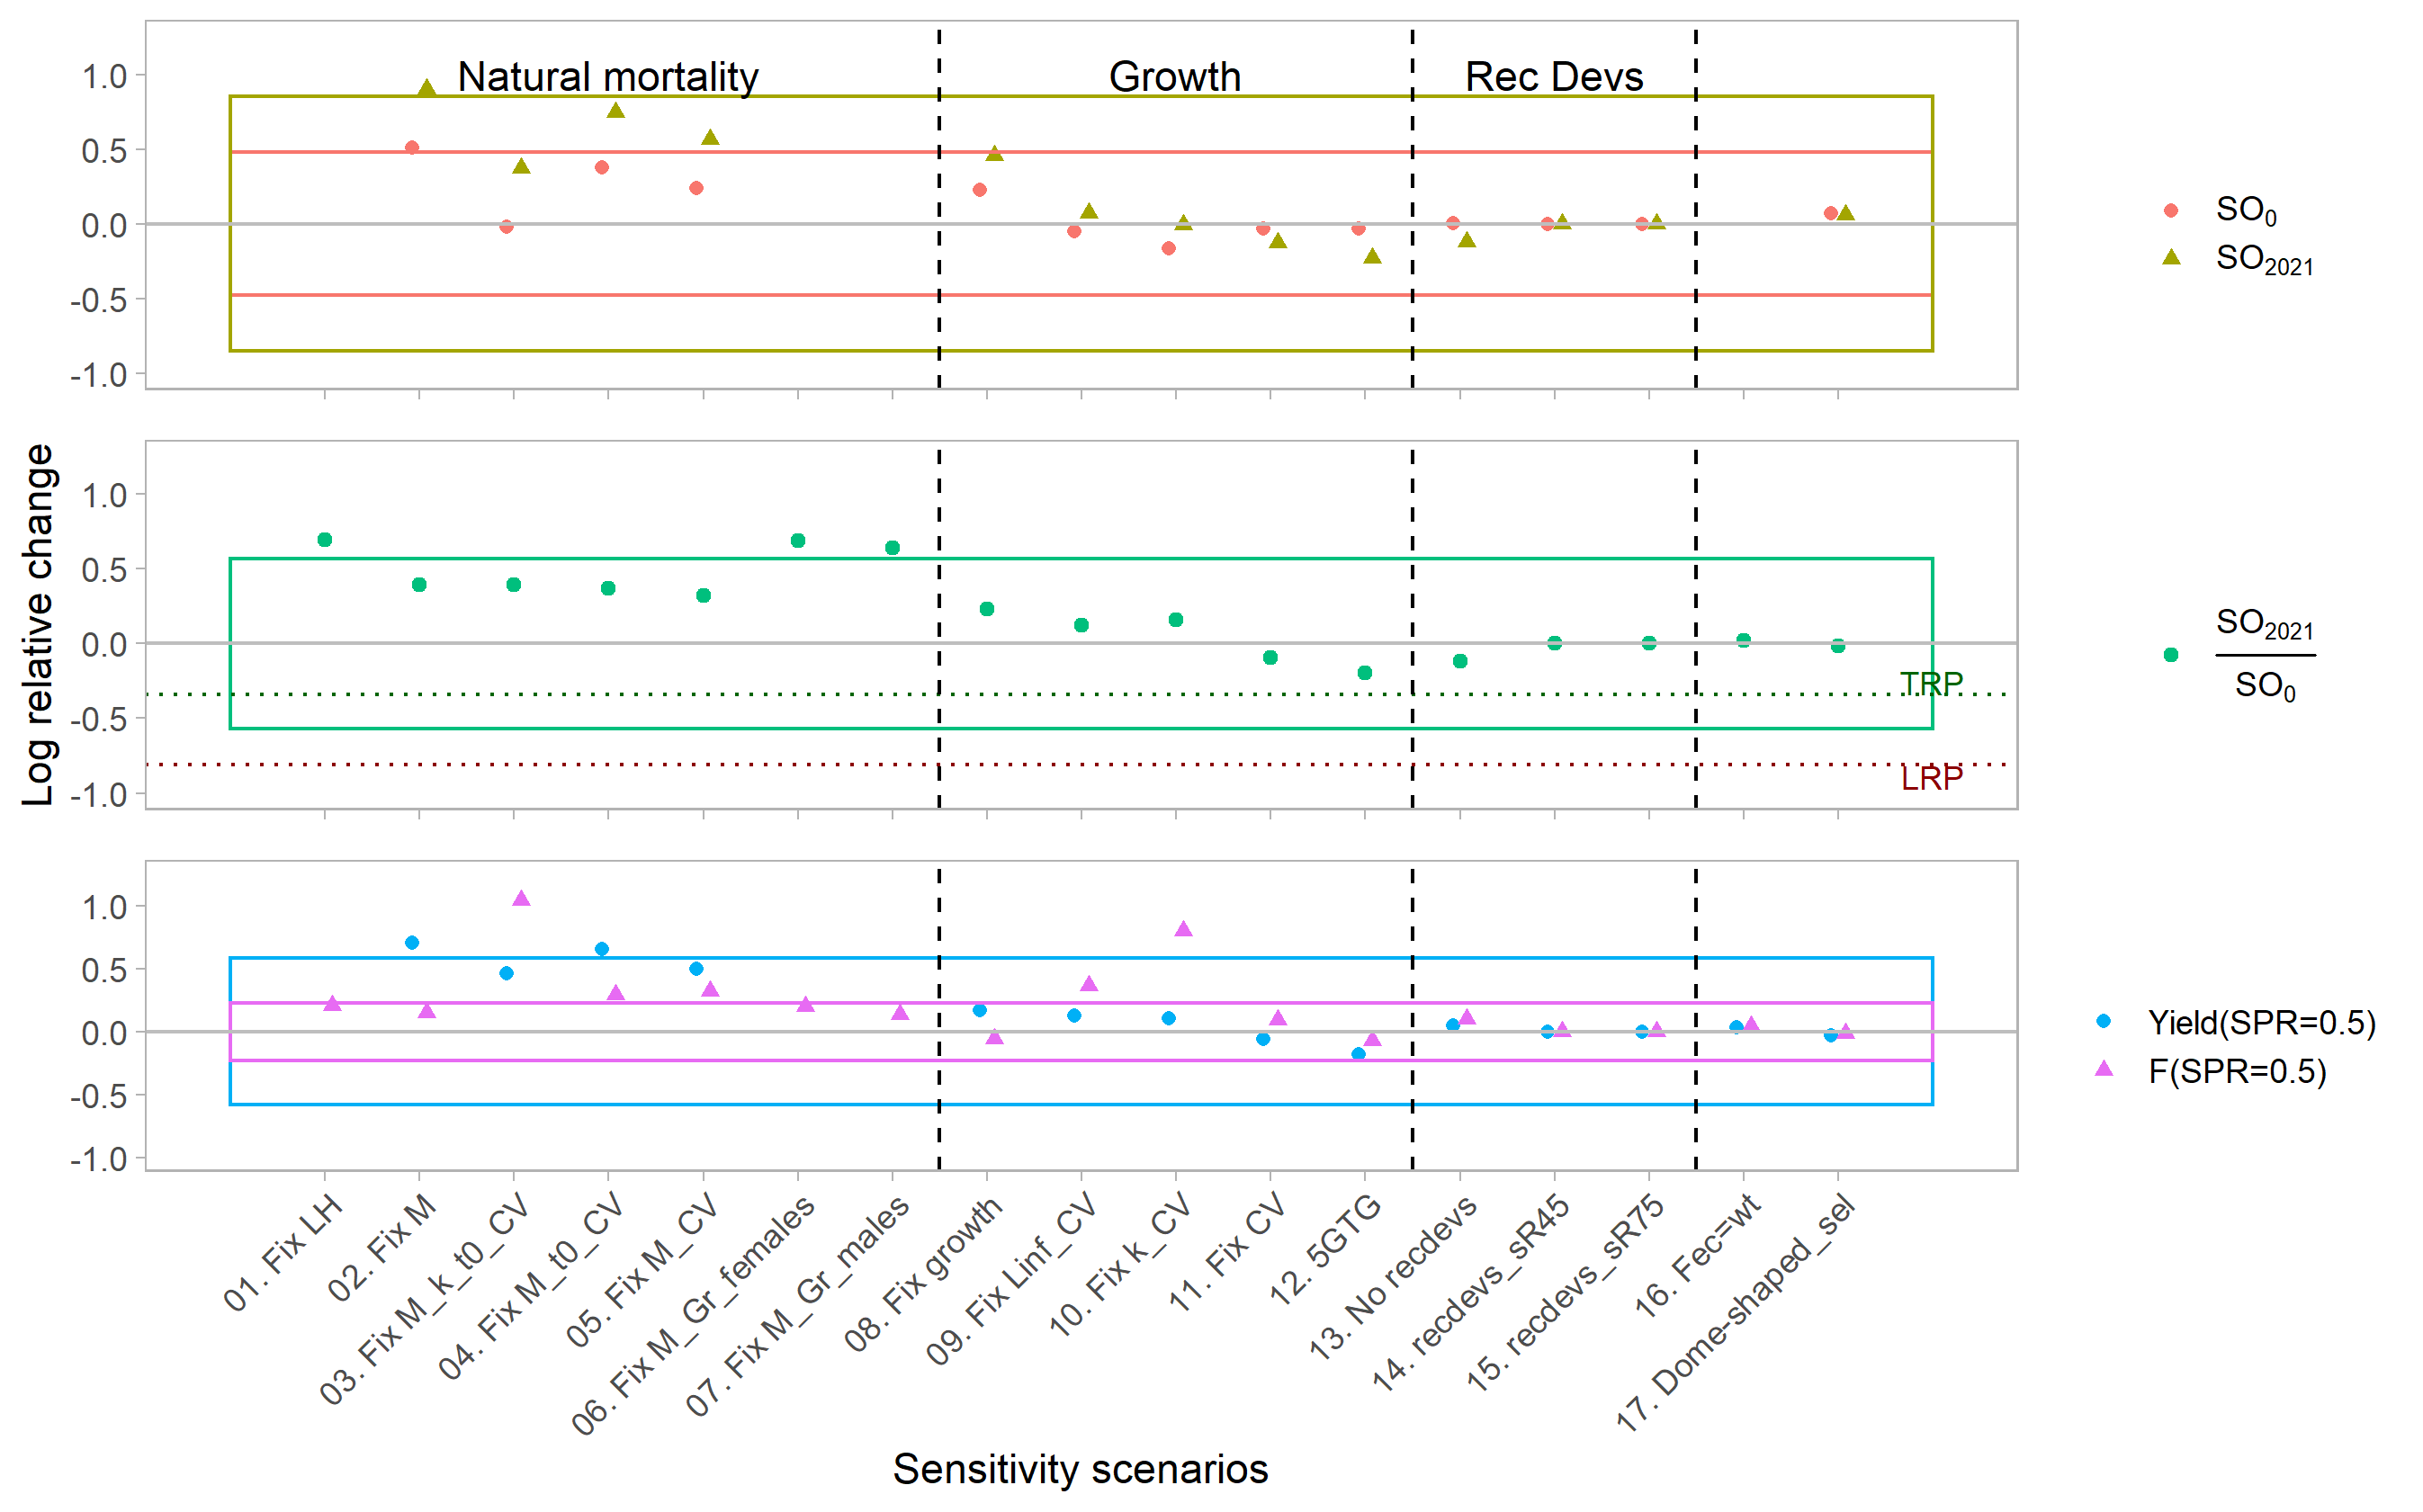
\includegraphics[width=1\textwidth,height=1\textheight]{C:/Users/Jason.Cope/Documents/Github/Vermilion rockfish OR WA assessment 2021/OR/write_up/figures/sensi_data/Sensi_logREplot_SB_Dep_F_MSY.png}
\caption{Log relative change (log((Model\_sensi-Model\_ref)/Model\_ref)) in data treatment for 5 derived quantities. Colored boxes indicate 95 percent confidence interval of the reference model.\label{fig:sensi-data-RE}}
\end{figure}

\tagmcend\tagstructend

\tagstructbegin{tag=Figure,alttext={Spawning biomass time series by data treatment compared to the reference model.}}\tagmcbegin{tag=Figure}

\begin{figure}
\centering
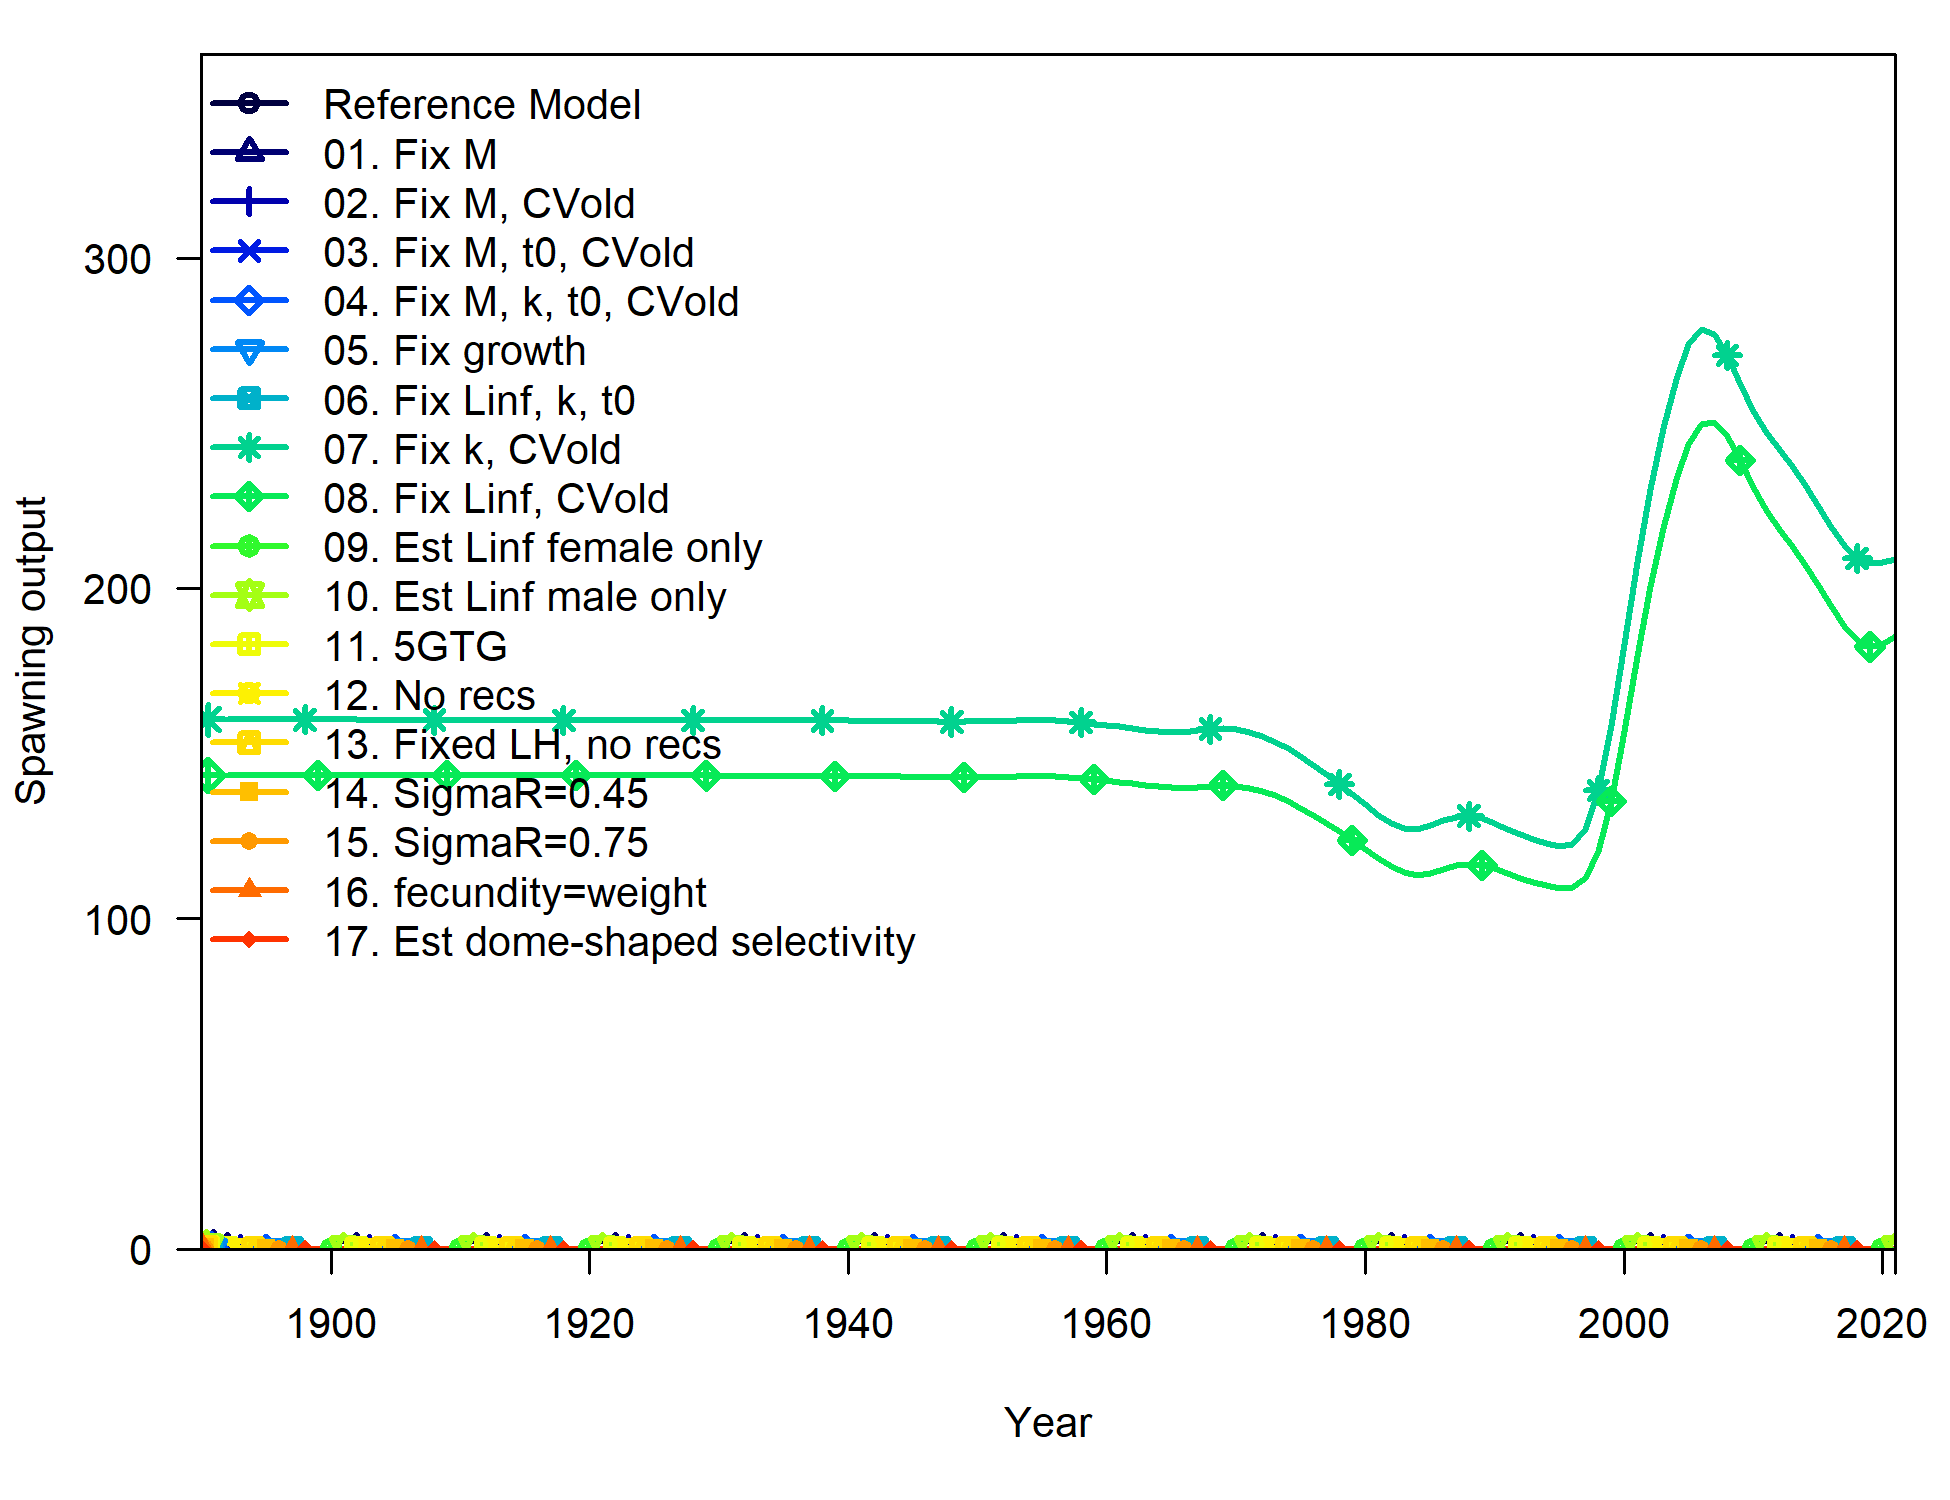
\includegraphics[width=1\textwidth,height=1\textheight]{C:/Users/Jason.Cope/Documents/Github/Vermilion rockfish OR WA assessment 2021/OR/write_up/figures/sensi_data/compare2_spawnbio_uncertainty.png}
\caption{Spawning biomass time series by data treatment compared to the reference model.\label{fig:sensi-data-ssb}}
\end{figure}

\tagmcend\tagstructend

\tagstructbegin{tag=Figure,alttext={Relative spawning biomass time series by data treatment compared to the reference model.}}\tagmcbegin{tag=Figure}

\begin{figure}
\centering
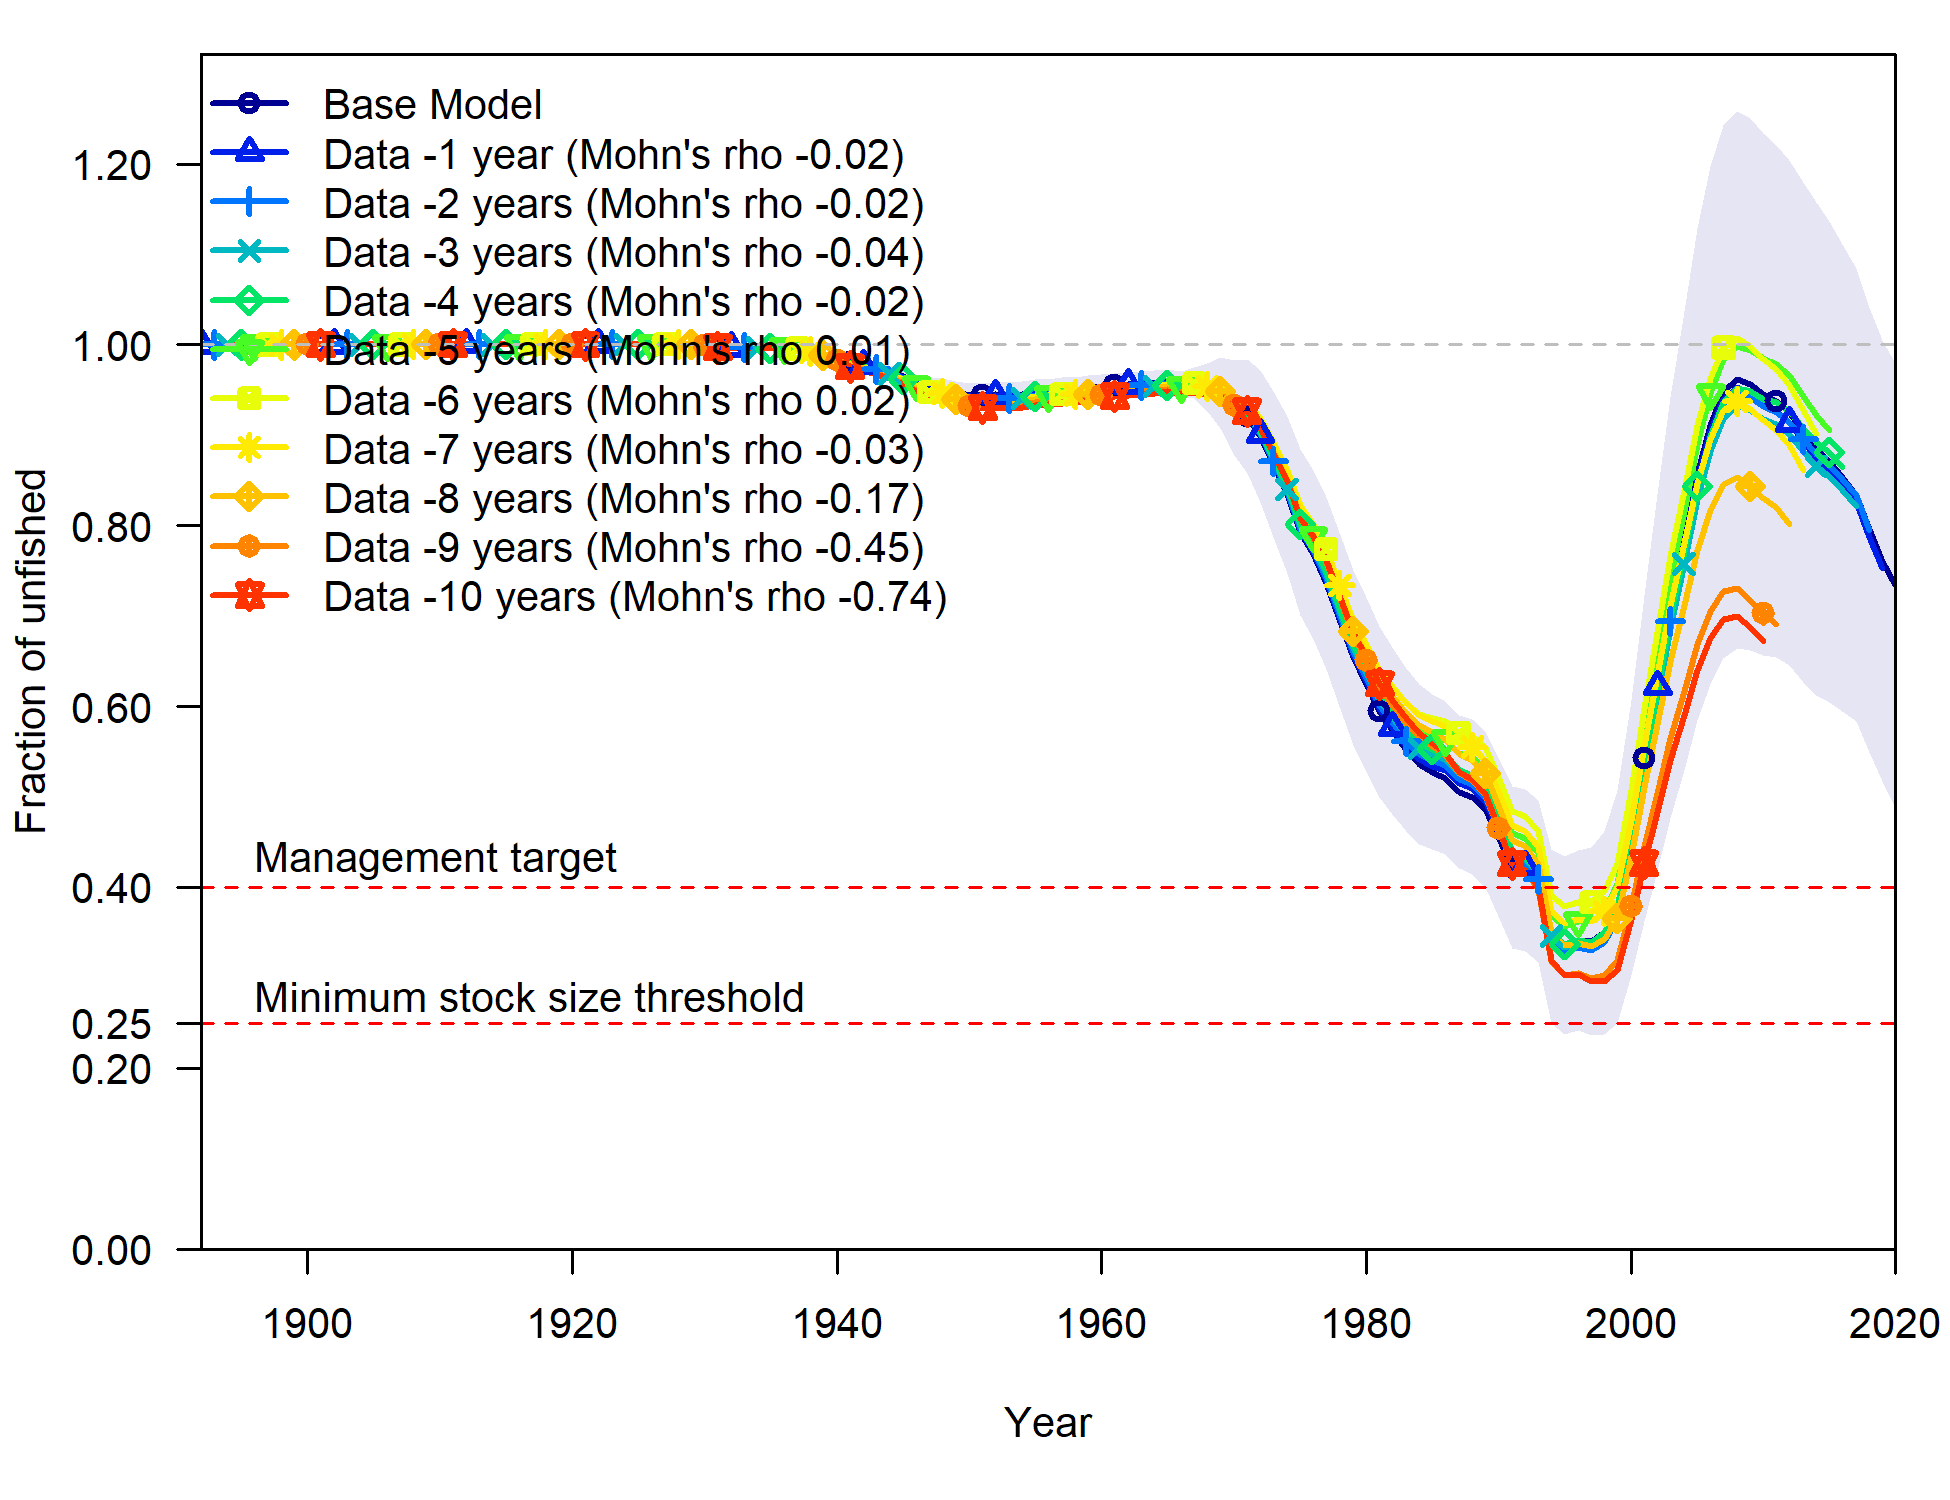
\includegraphics[width=1\textwidth,height=1\textheight]{C:/Users/Jason.Cope/Documents/Github/Vermilion rockfish OR WA assessment 2021/OR/write_up/figures/sensi_data/compare4_Bratio_uncertainty.png}
\caption{Relative spawning biomass time series by data treatment compared to the reference model.\label{fig:sensi-data-depl}}
\end{figure}

\tagmcend\tagstructend

\tagstructbegin{tag=Figure,alttext={Log relative change (log((Model_sensi-Model_ref)/Model_ref)) in data treatment for 5 derived quantities. Colored boxes indicate 95 percent confidence interval of the reference model.}}\tagmcbegin{tag=Figure}

\begin{figure}
\centering
\includegraphics[width=1\textwidth,height=1\textheight]{C:/Users/Jason.Cope/Documents/Github/Vermilion rockfish OR WA assessment 2021/OR/write_up/figures/sensi_data/Sensi_logREplot_SB_Dep_F_MSY.png}
\caption{Log relative change (log((Model\_sensi-Model\_ref)/Model\_ref)) in data treatment for 5 derived quantities. Colored boxes indicate 95 percent confidence interval of the reference model.\label{fig:sensi-modspec-RE}}
\end{figure}

\tagmcend\tagstructend

\tagstructbegin{tag=Figure,alttext={Spawning biomass time series by data treatment compared to the reference model.}}\tagmcbegin{tag=Figure}

\begin{figure}
\centering
\includegraphics[width=1\textwidth,height=1\textheight]{C:/Users/Jason.Cope/Documents/Github/Vermilion rockfish OR WA assessment 2021/OR/write_up/figures/sensi_data/compare2_spawnbio_uncertainty.png}
\caption{Spawning biomass time series by data treatment compared to the reference model.\label{fig:sensi-modspec-ssb}}
\end{figure}

\tagmcend\tagstructend

\tagstructbegin{tag=Figure,alttext={Relative spawning biomass time series by data treatment compared to the reference model.}}\tagmcbegin{tag=Figure}

\begin{figure}
\centering
\includegraphics[width=1\textwidth,height=1\textheight]{C:/Users/Jason.Cope/Documents/Github/Vermilion rockfish OR WA assessment 2021/OR/write_up/figures/sensi_data/compare4_Bratio_uncertainty.png}
\caption{Relative spawning biomass time series by data treatment compared to the reference model.\label{fig:sensi-modspec-depl}}
\end{figure}

\tagmcend\tagstructend

\tagstructbegin{tag=Figure,alttext={Estimated 1 - relative spawning ratio (SPR) by year.}}\tagmcbegin{tag=Figure}

\begin{figure}
\centering
\includegraphics[width=1\textwidth,height=1\textheight]{C:/Users/Jason.Cope/Documents/Github/Vermilion rockfish OR WA assessment 2021/OR/write_up/models/Reference model/plots/SPR2_minusSPRseries.png}
\caption{Estimated 1 - relative spawning ratio (SPR) by year.\label{fig:1-spr}}
\end{figure}

\tagmcend\tagstructend

\clearpage

\tagstructbegin{tag=Figure,alttext={Phase plot of the relative biomass (also referred to as fraction unfished) versus the SPR ratio where each point represents the biomass ratio at the start of the year and the relative fishing intensity in that same year. Lines through the final point show the 95 percent intervals based on the asymptotic uncertainty for each dimension. The shaded ellipse is a 95 percent region which accounts for the estimated correlations between the biomass ratio and SPR ratio.}}\tagmcbegin{tag=Figure}

\begin{figure}
\centering
\includegraphics[width=1\textwidth,height=1\textheight]{C:/Users/Jason.Cope/Documents/Github/Vermilion rockfish OR WA assessment 2021/OR/write_up/models/Reference model/plots/SPR4_phase.png}
\caption{Phase plot of the relative biomass (also referred to as fraction unfished) versus the SPR ratio where each point represents the biomass ratio at the start of the year and the relative fishing intensity in that same year. Lines through the final point show the 95 percent intervals based on the asymptotic uncertainty for each dimension. The shaded ellipse is a 95 percent region which accounts for the estimated correlations between the biomass ratio and SPR ratio.\label{fig:phase}}
\end{figure}

\tagmcend\tagstructend

\tagstructbegin{tag=Figure,alttext={Equilibrium yield curve for the base case model. Values are based on the 2020 fishery selectivities and with steepness fixed at 0.80.}}\tagmcbegin{tag=Figure}

\begin{figure}
\centering
\includegraphics[width=1\textwidth,height=1\textheight]{C:/Users/Jason.Cope/Documents/Github/Vermilion rockfish OR WA assessment 2021/OR/write_up/models/Reference model/plots/yield2_yield_curve_with_refpoints.png}
\caption{Equilibrium yield curve for the base case model. Values are based on the 2020 fishery selectivities and with steepness fixed at 0.80.\label{fig:yield}}
\end{figure}

\tagmcend\tagstructend

\clearpage

\tagstructbegin{tag=H1}\tagmcbegin{tag=H1}

\hypertarget{app-a}{%
\section{Appendix A: Detailed Fit to Length Composition Data}\label{app-a}}

\leavevmode\tagmcend\tagstructend

\tagstructbegin{tag=Figure,alttext={Length comps, whole catch, Commercial.<br><br>'N adj.' is the input sample size after data-weighting adjustment. N eff. is the calculated effective sample size used in the McAllister-Ianelli tuning method..}}\tagmcbegin{tag=Figure}

\begin{figure}
\centering
\includegraphics[width=1\textwidth,height=1\textheight]{C:/Users/Jason.Cope/Documents/Github/Vermilion rockfish OR WA assessment 2021/OR/write_up/models/Reference model/plots/comp_lenfit_flt1mkt0.png}
\caption{Length comps, whole catch, Commercial.`N adj.' is the input sample size after data-weighting adjustment. N eff. is the calculated effective sample size used in the McAllister-Ianelli tuning method..\label{fig:comp_lenfit_flt1mkt0}}
\end{figure}

\tagmcend\tagstructend

\tagstructbegin{tag=Figure,alttext={Length comps, whole catch, Recreational (plot 1 of 2).<br><br>'N adj.' is the input sample size after data-weighting adjustment. N eff. is the calculated effective sample size used in the McAllister-Ianelli tuning method..}}\tagmcbegin{tag=Figure}

\begin{figure}
\centering
\includegraphics[width=1\textwidth,height=1\textheight]{C:/Users/Jason.Cope/Documents/Github/Vermilion rockfish OR WA assessment 2021/OR/write_up/models/Reference model/plots/comp_lenfit_flt2mkt0_page1.png}
\caption{Length comps, whole catch, Recreational (plot 1 of 2).`N adj.' is the input sample size after data-weighting adjustment. N eff. is the calculated effective sample size used in the McAllister-Ianelli tuning method..\label{fig:comp_lenfit_flt2mkt0_page1}}
\end{figure}

\tagmcend\tagstructend

\tagstructbegin{tag=Figure,alttext={Length comps, whole catch, Recreational (plot 2 of 2).}}\tagmcbegin{tag=Figure}

\begin{figure}
\centering
\includegraphics[width=1\textwidth,height=1\textheight]{C:/Users/Jason.Cope/Documents/Github/Vermilion rockfish OR WA assessment 2021/OR/write_up/models/Reference model/plots/comp_lenfit_flt2mkt0_page2.png}
\caption{Length comps, whole catch, Recreational (plot 2 of 2).\label{fig:comp_lenfit_flt2mkt0_page2}}
\end{figure}

\tagmcend\tagstructend

\clearpage

\tagstructbegin{tag=H1}\tagmcbegin{tag=H1}

\hypertarget{app-b}{%
\section{Appendix B: Detailed Fit to Conditional-Age-at-Length Composition Data}\label{app-b}}

\leavevmode\tagmcend\tagstructend

\tagstructbegin{tag=Figure,alttext={Pearson residuals, whole catch, Commercial (max=30.56) (plot 1 of 4) (plot 2 of 4).}}\tagmcbegin{tag=Figure}

\begin{figure}
\centering
\includegraphics[width=1\textwidth,height=1\textheight]{C:/Users/Jason.Cope/Documents/Github/Vermilion rockfish OR WA assessment 2021/OR/write_up/models/Reference model/plots/comp_condAALfit_residsflt1mkt0_page2.png}
\caption{Pearson residuals, whole catch, Commercial (max=30.56) (plot 1 of 4) (plot 2 of 4).\label{fig:comp_condAALfit_residsflt1mkt0_page2}}
\end{figure}

\tagmcend\tagstructend

\tagstructbegin{tag=Figure,alttext={Pearson residuals, whole catch, Commercial (max=30.56) (plot 1 of 4) (plot 2 of 4) (plot 3 of 4).}}\tagmcbegin{tag=Figure}

\begin{figure}
\centering
\includegraphics[width=1\textwidth,height=1\textheight]{C:/Users/Jason.Cope/Documents/Github/Vermilion rockfish OR WA assessment 2021/OR/write_up/models/Reference model/plots/comp_condAALfit_residsflt1mkt0_page3.png}
\caption{Pearson residuals, whole catch, Commercial (max=30.56) (plot 1 of 4) (plot 2 of 4) (plot 3 of 4).\label{fig:comp_condAALfit_residsflt1mkt0_page3}}
\end{figure}

\tagmcend\tagstructend

\tagstructbegin{tag=Figure,alttext={Pearson residuals, whole catch, Commercial (max=30.56) (plot 1 of 4) (plot 2 of 4) (plot 3 of 4) (plot 4 of 4).}}\tagmcbegin{tag=Figure}

\begin{figure}
\centering
\includegraphics[width=1\textwidth,height=1\textheight]{C:/Users/Jason.Cope/Documents/Github/Vermilion rockfish OR WA assessment 2021/OR/write_up/models/Reference model/plots/comp_condAALfit_residsflt1mkt0_page4.png}
\caption{Pearson residuals, whole catch, Commercial (max=30.56) (plot 1 of 4) (plot 2 of 4) (plot 3 of 4) (plot 4 of 4).\label{fig:comp_condAALfit_residsflt1mkt0_page4}}
\end{figure}

\tagmcend\tagstructend

\tagstructbegin{tag=Figure,alttext={Pearson residuals, whole catch, Recreational (max=30.63) (plot 1 of 3).}}\tagmcbegin{tag=Figure}

\begin{figure}
\centering
\includegraphics[width=1\textwidth,height=1\textheight]{C:/Users/Jason.Cope/Documents/Github/Vermilion rockfish OR WA assessment 2021/OR/write_up/models/Reference model/plots/comp_condAALfit_residsflt2mkt0_page1.png}
\caption{Pearson residuals, whole catch, Recreational (max=30.63) (plot 1 of 3).\label{fig:comp_condAALfit_residsflt2mkt0_page1}}
\end{figure}

\tagmcend\tagstructend

\tagstructbegin{tag=Figure,alttext={Pearson residuals, whole catch, Recreational (max=30.63) (plot 1 of 3) (plot 2 of 3).}}\tagmcbegin{tag=Figure}

\begin{figure}
\centering
\includegraphics[width=1\textwidth,height=1\textheight]{C:/Users/Jason.Cope/Documents/Github/Vermilion rockfish OR WA assessment 2021/OR/write_up/models/Reference model/plots/comp_condAALfit_residsflt2mkt0_page2.png}
\caption{Pearson residuals, whole catch, Recreational (max=30.63) (plot 1 of 3) (plot 2 of 3).\label{fig:comp_condAALfit_residsflt2mkt0_page2}}
\end{figure}

\tagmcend\tagstructend

\tagstructbegin{tag=Figure,alttext={Pearson residuals, whole catch, Recreational (max=30.63) (plot 1 of 3) (plot 2 of 3) (plot 3 of 3).}}\tagmcbegin{tag=Figure}

\begin{figure}
\centering
\includegraphics[width=1\textwidth,height=1\textheight]{C:/Users/Jason.Cope/Documents/Github/Vermilion rockfish OR WA assessment 2021/OR/write_up/models/Reference model/plots/comp_condAALfit_residsflt2mkt0_page3.png}
\caption{Pearson residuals, whole catch, Recreational (max=30.63) (plot 1 of 3) (plot 2 of 3) (plot 3 of 3).\label{fig:comp_condAALfit_residsflt2mkt0_page3}}
\end{figure}

\tagmcend\tagstructend

\clearpage

\tagstructbegin{tag=H1}\tagmcbegin{tag=H1}

\hypertarget{app-c}{%
\section{Appendix C: Detailed Fit to Conditional-Age-at-Length Composition Data}\label{app-c}}

\leavevmode\tagmcend\tagstructend

\tagstructbegin{tag=Figure,alttext={Pearson residuals, whole catch, Commercial (max=30.56) (plot 1 of 4) (plot 2 of 4).}}\tagmcbegin{tag=Figure}

\begin{figure}
\centering
\includegraphics[width=1\textwidth,height=1\textheight]{C:/Users/Jason.Cope/Documents/Github/Vermilion rockfish OR WA assessment 2021/OR/write_up/models/Reference model/plots/comp_condAALfit_residsflt1mkt0_page2.png}
\caption{Pearson residuals, whole catch, Commercial (max=30.56) (plot 1 of 4) (plot 2 of 4).\label{fig:comp_condAALfit_residsflt1mkt0_page2}}
\end{figure}

\tagmcend\tagstructend

\tagstructbegin{tag=Figure,alttext={Pearson residuals, whole catch, Commercial (max=30.56) (plot 1 of 4) (plot 2 of 4) (plot 3 of 4).}}\tagmcbegin{tag=Figure}

\begin{figure}
\centering
\includegraphics[width=1\textwidth,height=1\textheight]{C:/Users/Jason.Cope/Documents/Github/Vermilion rockfish OR WA assessment 2021/OR/write_up/models/Reference model/plots/comp_condAALfit_residsflt1mkt0_page3.png}
\caption{Pearson residuals, whole catch, Commercial (max=30.56) (plot 1 of 4) (plot 2 of 4) (plot 3 of 4).\label{fig:comp_condAALfit_residsflt1mkt0_page3}}
\end{figure}

\tagmcend\tagstructend

\tagstructbegin{tag=Figure,alttext={Pearson residuals, whole catch, Commercial (max=30.56) (plot 1 of 4) (plot 2 of 4) (plot 3 of 4) (plot 4 of 4).}}\tagmcbegin{tag=Figure}

\begin{figure}
\centering
\includegraphics[width=1\textwidth,height=1\textheight]{C:/Users/Jason.Cope/Documents/Github/Vermilion rockfish OR WA assessment 2021/OR/write_up/models/Reference model/plots/comp_condAALfit_residsflt1mkt0_page4.png}
\caption{Pearson residuals, whole catch, Commercial (max=30.56) (plot 1 of 4) (plot 2 of 4) (plot 3 of 4) (plot 4 of 4).\label{fig:comp_condAALfit_residsflt1mkt0_page4}}
\end{figure}

\tagmcend\tagstructend

\tagstructbegin{tag=Figure,alttext={Pearson residuals, whole catch, Recreational (max=30.63) (plot 1 of 3).}}\tagmcbegin{tag=Figure}

\begin{figure}
\centering
\includegraphics[width=1\textwidth,height=1\textheight]{C:/Users/Jason.Cope/Documents/Github/Vermilion rockfish OR WA assessment 2021/OR/write_up/models/Reference model/plots/comp_condAALfit_residsflt2mkt0_page1.png}
\caption{Pearson residuals, whole catch, Recreational (max=30.63) (plot 1 of 3).\label{fig:comp_condAALfit_residsflt2mkt0_page1}}
\end{figure}

\tagmcend\tagstructend

\tagstructbegin{tag=Figure,alttext={Pearson residuals, whole catch, Recreational (max=30.63) (plot 1 of 3) (plot 2 of 3).}}\tagmcbegin{tag=Figure}

\begin{figure}
\centering
\includegraphics[width=1\textwidth,height=1\textheight]{C:/Users/Jason.Cope/Documents/Github/Vermilion rockfish OR WA assessment 2021/OR/write_up/models/Reference model/plots/comp_condAALfit_residsflt2mkt0_page2.png}
\caption{Pearson residuals, whole catch, Recreational (max=30.63) (plot 1 of 3) (plot 2 of 3).\label{fig:comp_condAALfit_residsflt2mkt0_page2}}
\end{figure}

\tagmcend\tagstructend

\tagstructbegin{tag=Figure,alttext={Pearson residuals, whole catch, Recreational (max=30.63) (plot 1 of 3) (plot 2 of 3) (plot 3 of 3).}}\tagmcbegin{tag=Figure}

\begin{figure}
\centering
\includegraphics[width=1\textwidth,height=1\textheight]{C:/Users/Jason.Cope/Documents/Github/Vermilion rockfish OR WA assessment 2021/OR/write_up/models/Reference model/plots/comp_condAALfit_residsflt2mkt0_page3.png}
\caption{Pearson residuals, whole catch, Recreational (max=30.63) (plot 1 of 3) (plot 2 of 3) (plot 3 of 3).\label{fig:comp_condAALfit_residsflt2mkt0_page3}}
\end{figure}

\tagmcend\tagstructend
\end{document}
